\documentclass[12pt, a4paper]{book} 

% =========================
% PREAMBLE (preamble.tex)
% =========================

% --- Dil ve kodlama: bunlar en başta olsun ---
\usepackage[T1]{fontenc}
\usepackage[utf8]{inputenc}
\usepackage[turkish,shorthands=off]{babel}


% --- Özet (book sınıfı için) ---
\newcommand{\abstractname}{Özet}
\newenvironment{abstract}{
  \cleardoublepage
  \thispagestyle{plain}
  \chapter*{\abstractname}
  \addcontentsline{toc}{chapter}{\abstractname}
}{\cleardoublepage}


% --- Yazı tipi ve mikro tipografi (önerilir) ---
\usepackage{lmodern}
%\let\CheckCommand\providecommand
%\usepackage{microtype}

% --- Sayfa yerleşimi ---
\usepackage{geometry}
\geometry{margin=2.5cm}

% --- Matematik ve semboller ---
\usepackage{amsmath, amssymb, bm}

% --- Grafik, çizim, tablo ---
\usepackage{graphicx}
\usepackage{float}
\usepackage{tabularx}
\usepackage{longtable}
\usepackage{array}
\usepackage{booktabs}
\usepackage{tikz}
\usepackage{xcolor}
\usetikzlibrary{decorations.pathmorphing}
\usetikzlibrary{arrows.meta,positioning,shapes.geometric,fit,calc}
\usepackage{fvextra}
\usepackage{dirtree}


% --- Kutular / renkli çerçeveler ---
% not: 'tcolor' değil 'tcolorbox' olmalı
\usepackage[most]{tcolorbox}

% --- Diğer yardımcılar ---
\usepackage[normalem]{ulem}
\usepackage{comment}

\usepackage[
  backend=biber,
  style=ieee,
  maxbibnames=3,
  maxcitenames=2,
  giveninits=true,
  doi=false,
  url=false,
  isbn=false
]{biblatex}

\addbibresource{references.bib}

\usepackage{caption}
\usepackage{algorithm}
\usepackage{algorithmic}

% --- Hiperbağlantılar (en sonda yüklensin) ---
\usepackage{hyperref}
\hypersetup{
    unicode=true,           % Türkçe karakterler için
    colorlinks=true,
    linkcolor=black,
    filecolor=black,
    urlcolor=black,
    citecolor=black,
    pdftitle={Başlık},
    pdfauthor={Yazar}
}

% preamble.tex içinde
\usepackage{graphicx}
\usepackage{eso-pic}

\newcommand{\CoverBackground}{%
  \AddToShipoutPictureBG*{%
    \AtPageLowerLeft{%
      \includegraphics[width=\paperwidth,height=\paperheight]{Resimler/Yerçekimi Modelleri.png}%  % Kapa Tasarımı.png dosyasını KapaTasarimi.png yap
    }%
  }%
}

\newcommand{\volume}{{\ooalign{\hfil$V$\hfil\cr\kern0.08em--\hfil\cr}}} 

\author{Ayberk Demirkanat} 
\title{\textbf{Küresel Harmonikler}} 
\date{} 

\begin{document}

\begin{titlepage}
    % Arka plan resmi
    \CoverBackground

    % Üstten itibaren yüksekliği elle ayarla (0.8 -> sayfanın %80'i)
    \vspace*{0.92\textheight}

    % Aşağı ORTADA, beyazımsı renkte not
    \begin{center}
        {\textcolor{white!80!yellow!10}{\large Ayberk Demirkanat \\ Not Serisi}}
    \end{center}

\end{titlepage}

\ClearShipoutPictureBG



\begin{abstract}
Bu çalışma, yerçekimi alanlarının küresel harmonikler kullanılarak modellenmesini ve bu
modellerin yörünge dinamiği ile uzay görevi tasarımı üzerindeki etkilerinin bütüncül bir
çerçevede incelenmesini amaçlamaktadır.

\paragraph{İlk Bölümde} küresel harmonik açılımın matematiksel temelini oluşturan Legendre
polinomlarının ortaya çıkışı ele alınmış; bu polinomların Legendre diferansiyel denklemi ile
ilişkisi, ortonormallik özellikleri ve seri açılım katsayılarının projeksiyon temelli yöntemlerle
nasıl elde edildiği ayrıntılı olarak açıklanmıştır. Bu bölüm, potansiyel teorisinden enlem ve
boylam bağımlılığı içeren küresel harmonik gösterime geçiş için gerekli kuramsal altyapıyı
oluşturmaktadır.

\paragraph{İkinci Bölümde} Dünya’nın mükemmel küre varsayımından sapmasının neden olduğu
yerçekimi alanı düzensizlikleri incelenmiştir. Özellikle Dünya’nın basıklığı ve kütle
dağılımındaki bölgesel farklılıkların yerçekimi potansiyeline ek terimler olarak nasıl yansıdığı
gösterilmiş; zonal, tesseral ve sektörel harmonik bileşenlerin fiziksel anlamları üzerinden bu
katsayıların yörünge elemanlarında zamana bağlı pertürbasyonlara nasıl yol açtığı
tartışılmıştır. Ayrıca, farklı görev profilleri için gravite modeli derece ve mertebe seçiminde
doğruluk, kararlılık ve hesaplama maliyeti arasındaki denge değerlendirilmiştir.

\paragraph{Üçüncü Bölümde} Ay çevresinde gözlenen belirgin yerçekimi anomalilerinin, özellikle
mascon yapılarının, kökeni ve bu anomalilerin uzay görevleri üzerindeki etkileri ele alınmıştır.
Ay yerçekimi alanının ölçülmesinde kullanılan başlıca yöntemler özetlenmiş; Ay görevleri için
uygun gravite modelinin seçiminde dikkate alınması gereken irtifa, hassasiyet ve uzun süreli
yörünge kararlılığı gibi kriterler tartışılmıştır. Ayrıca, seçilen gravite modellerinin dinamik
tutarlılığının test edilmesi amacıyla yörünge propagasyonu, artık hata analizi ve karşılaştırmalı
senaryolar gibi doğrulama yaklaşımları sunulmuştur.

\paragraph{Dördüncü Bölümde} kuramsal gravite modellemesinin mühendislik uygulamasına
aktarımı hedeflenerek sayısal hesaplama ve simülasyon akışı ele alınmıştır: Cowell yöntemi ile
hareket denklemlerinin doğrudan entegrasyonu, senaryoya uygun integratör seçimi (örn. RK45,
yüksek mertebeli DOP853/RK89 ve uzun süreli kararlılık için simplektik yaklaşımlar) ve hata
toleransı ayarları tartışılmıştır. Ayrıca, görev tasarımında standart prosedür kapsamında gravite katsayılarının yüklenmesi, propagasyonun yürütülmesi, çıktıların
yörünge elemanlarına dönüştürülmesi ve modelin doğrulanması/karşılaştırılması (V\&V) adımları; enerji/yarı-büyük eksen davranışı ve analitik $J_2$ sağlama kontrolleri gibi pratik
kriterlerle birlikte sunulmuştur.

\paragraph{Beşinci Bölümde}, Python ile geliştirilen Ay simülasyon projesinde 
fiziksel sadakati artırmaya yönelik ileri pertürbasyonlar ve çevresel etkileşimler 
ele alınmıştır. Bu kapsamda, NASA SPICE efemerisleri kullanılarak Güneş/Dünya üçüncü 
cisim etkileri modele entegre edilmiş; SRP hesaplarında Ay’ın gölge konisi (umbra/penumbra) 
konik geometriyle hassas biçimde modellenmiş; Ay kaynaklı Albedo ve Termal IR itkilerinin 
dinamiğe katkısı incelenmiştir. Ayrıca milimetre ölçeğinde doğruluk için 1PN genel görelilik 
düzeltmeleri ve solid-body tides gibi yüksek sadakatli bileşenlerin matematiksel altyapısı sunulmuştur. 
Görev emniyeti açısından kritik olan impact detection sürecinde ise, yüzey teması basit bir referans küre 
yerine LRO/LOLA sayısal yükseklik modeli (DEM) üzerinden arazi duyarlı şekilde tespit edilmiş ve büyük veri 
setleri mmap yöntemiyle bellek verimli biçimde yönetilmiştir. Bölüm sonunda, tüm bu etkilerin yörünge 
kararlılığı, yer izi ve görev ömrü üzerindeki kümülatif sonuçları otomatik post-process, profesyonel PDF 
raporlama ve yüksek çözünürlüklü 3D animasyon çıktılarıyla değerlendirilmiştir.

\medskip
Bu yönüyle çalışma, Dünya ve Ay için gravite modellemesi ile yörünge analizi arasında doğrudan bir mühendislik 
bağı kurmayı hedeflemektedir. İdealize edilmiş iki-cisim yaklaşımından uzaklaşarak; Ay’ın mascon kaynaklı 
heterojen kütle dağılımını, NASA SPICE tabanlı hassas efemeris verilerini ve gerçek topografik verileri aynı 
dinamik çerçevede birleştirmektedir. Geliştirilen bu yüksek sadakatli (high-fidelity) simülasyon altyapısı, kuramsal 
geopotansiyel teorisinin operasyonel görev tasarım süreçlerine hatasız bir şekilde entegre edilmesini sağlayarak, 
doğrulanabilir, performans odaklı ve akademik derinliği haiz bir yörünge analiz platformu sunmaktadır.
\end{abstract}


\cleardoublepage

% =========== Notasyon ==========
% =================== Kullanılan Notasyonlar ===================
\chapter*{Kullanılan Notasyonlar}
\addcontentsline{toc}{chapter}{Kullanılan Notasyonlar}

Bu çalışmada yerçekimi alanlarının küresel harmonikler kullanılarak modellenmesi kapsamında aşağıda verilen notasyonlar kullanılmıştır. Semboller, metin boyunca tutarlı olacak şekilde tanımlanmış olup, aksi belirtilmedikçe skaler büyüklükleri temsil etmektedir.

\medskip
Özellikle Legendre polinomları ve ilişkili fonksiyonlarda, fonksiyonel bağımlılığın cebirsel çarpma işlemleriyle karıştırılmasını önlemek ve matematiksel okunabilirliği
artırmak amacıyla, fonksiyon argümanları standart parantez $()$ yerine köşeli parantez $[]$ ile (örneğin $P_{\ell}^{m}[\sin\phi_{gc}]$) gösterilmiştir.

\vspace{0.4cm}

\setlength{\LTpre}{0pt}
\setlength{\LTpost}{0pt}
\renewcommand{\arraystretch}{1.15}

\begin{longtable}{>{\raggedright\arraybackslash}p{3.2cm} p{10.8cm}}
\toprule
\textbf{Sembol} & \textbf{Açıklama} \\
\midrule
\endfirsthead

\toprule
\textbf{Sembol} & \textbf{Açıklama} \\
\midrule
\endhead

\midrule
\multicolumn{2}{r}{\emph{(devam ediyor)}}\\
\endfoot

\bottomrule
\endlastfoot

$r$ & Cisim merkezinden ölçülen radyal uzaklık (skaler) \\
$\mathbf{r}$ & Konum vektörü \\

$R_E$ & Dünya için referans yarıçapı \\
$R_M$ & Ay için referans yarıçapı \\
$R_{\text{ref}}$ & Genel referans yarıçapı (model bazlı; Dünya/Ay) \\

$\phi_{gc}$ & Geosentrik enlem \\
$\lambda$ & Boylam \\
$\theta$ & Kolatitude ($\theta=\tfrac{\pi}{2}-\phi_{gc}$) \\
$x$ & Legendre argümanı ($x=\cos\theta=\sin\phi_{gc}$) \\

$U$ & Yerçekimi potansiyeli \\
$\mu$ & Standart çekim parametresi ($\mu = GM$) \\
$G$ & Evrensel çekim sabiti \\
$M$ & Gökcisminin kütlesi \\

$P_{\ell}[x]$ & $\ell$ dereceli Legendre polinomu \\
$P_{\ell}^{m}[x]$ &
$\ell$ derece, $m$ mertebeli ilişkili Legendre fonksiyonu (Condon--Shortley fazı hariç) \\
$P_{\ell}^{m,\mathrm{CS}}[x]$ &
Condon--Shortley fazını içeren tanım ($P_{\ell}^{m,\mathrm{CS}}[x]=(-1)^m P_{\ell}^{m}[x]$) \\

$\overline{P}_{\ell}^{m}[x]$ &
Tam-normalize edilmiş ilişkili Legendre fonksiyonu (real harmonikler) \\
$N_{\ell,m}$ & Normalizasyon çarpanı ($\overline{P}_{\ell}^{m}=N_{\ell,m}P_{\ell}^{m}$) \\

$\ell$ & Küresel harmonik derecesi (degree) \\
$m$ & Küresel harmonik mertebesi (order) \\

$C_{\ell,m}$ & Kosinüs küresel harmonik katsayısı (normalize edilmemiş baz ile uyumlu) \\
$S_{\ell,m}$ & Sinüs küresel harmonik katsayısı (normalize edilmemiş baz ile uyumlu) \\
$\overline{C}_{\ell,m}$ & Tam-normalize edilmiş kosinüs katsayısı (EGM/jeodezik konvansiyon) \\
$\overline{S}_{\ell,m}$ & Tam-normalize edilmiş sinüs katsayısı (EGM/jeodezik konvansiyon) \\

$J_{\ell}$ & Zonal harmonik katsayısı ($m=0$ terimleri ile ilişkili) \\

$d_Q$ & Gözlem noktası ile kütle elemanı arasındaki mesafe (skaler) \\

$\mathbf{a}$ & Yerçekimi ivme vektörü \\

\end{longtable}

\vspace{0.2cm}

Bu notasyonlar, Dünya ve Ay için kullanılan tüm gravite modelleri ve yörünge
analizlerinde ortak bir referans çerçevesi sağlamak amacıyla tanımlanmıştır.


% ======= İçindekiler ========
\tableofcontents


% ============ Legendre Polinomları ============
\chapter{Legendre Polinomları}

\section{Giriş}

\medskip
\noindent
\textbf{Bölümün Kapsamı ve Yol Haritası.}
Bu bölümde sırasıyla:
(i) Legendre diferansiyel denklemi ve $P_n(x)$ ailesinin tanımı,
(ii) ortogonallik ve seri açılım katsayılarının projeksiyon mantığıyla elde edilmesi,
(iii) potansiyel teorisi bağlamında sferik harmoniklere geçiş ve fiziksel yorumlar
düzenli bir çerçevede sunulacaktır.


% ============== Tarihçesi ve Motivasyonu ==============
\newpage
\section{Tarihçesi ve Motivasyonu}

Legendre polinomları, matematikteki en temel \textbf{ortogonal polinom aileleri}nden biridir. Bugün yalnızca çekim alanı problemlerinde değil; potansiyel teorisi, elektrostatik,
manyetostatik, ısı iletimi/difüzyon, dalga yayılımı, kuantum mekaniği (özellikle açısal momentum ve küresel simetri),
sayısal analiz (Gauss--Legendre integrasyonu) ve PDE çözümleri (değişkenlerin ayrılması) gibi çok geniş bir alanda karşımıza çıkar.

\medskip
Bu çeşitliliğin ortak nedeni: küresel veya eksenel simetri içeren sistemlerde açısal bağımlılığı düzenli, kararlı ve sistematik biçimde temsil eden doğal baz fonksiyonları olmalarıdır.

\medskip
Yerçekimi ve yörünge mekaniği bağlamında, gerçek gökcisimlerinin (Dünya dâhil) mükemmel küre olmaması nedeniyle ortaya çıkan şekil bozuklukları ve kütle dağılımındaki düzensizlikler, küçük görünse bile hassas yörünge hesaplarında birikimli etkiler üretir. Bu nedenle temel soru şudur:

\begin{quote}
Küresel olmayan bir kütle dağılımının uzayda oluşturduğu çekim potansiyeli,
yeterli doğrulukta ve sistematik biçimde nasıl ifade edilir?
\end{quote}

Pratik yaklaşım, potansiyeli tek adımda kapalı bir integral formunda ifade etmek yerine, onu \textbf{düzenli bir seri açılımı}yla bileşenlerine ayırmaktır. Bu açılımın açısal kısmında Legendre polinomlarının belirmesi tesadüf değildir: uygun koordinatlarda problem ayrıştırıldığında açısal bağımlılık, tam olarak bu polinomların çözdüğü diferansiyel denkleme indirgenir.
Aşağıda bu ihtiyacın tarihsel olarak nasıl olgunlaştığı özetlenmiştir.

% -------------- Newton ve Küre Modeli ------------
\paragraph{1. Newton ve Küre Modeli (1687):}
Isaac Newton, \emph{Principia} (1687) adlı eserinde homojen bir kürenin, dış uzaydaki çekim etkisinin, tüm kütlesi merkezde toplanmış tek bir noktasal kütleninkiyle aynı olduğunu gösterdi. Bu yüzden küre dışındaki bir noktada yerçekimi potansiyeli,
merkezi çekim formunda

\begin{equation}
U(\mathbf{r})=-\frac{\mu}{\lVert \mathbf{r}\rVert},
\qquad \mu \equiv GM.
\label{eq:pointmass_potential}
\end{equation}

şeklinde yazılabilir. Bu idealizasyon yerçekimi problemlerine güçlü ve sade bir başlangıç sunsa da, Dünya’nın dönmeye bağlı basıklığı ve kütle dağılımındaki düzensizlikler nedeniyle
gerçek alan bu basit modelden düzenli olarak sapar. Dolayısıyla daha yüksek doğruluk için merkezi potansiyelin üzerine  \textbf{küresel olmayan} (\emph{asferik}) düzeltmeler eklemek gerekir.

% ------------- Dünyanın Şekli Üzerine Tartışmalar ----------
\paragraph{2. Dünya’nın Şekli Üzerine Tartışmalar (1700'ler)}
Dünya’nın dönmesi, merkezkaç etkisi nedeniyle yaklaşık olarak \textbf{kutuplardan basık} (\emph{oblate}) bir denge şekline işaret eder. Nitekim Newton (ve aynı dönemde Huygens) dönmenin Dünya’yı kutuplardan basıklaştıracağını öngörürken,
Cassini ailesinin Fransa’daki erken meridyen yayı ölçümlerine dayanan yorumu bir süre Dünya’nın \textbf{kutuplardan uzun} (\emph{prolate}) olabileceği yönünde bir karşı görüşü beslemiştir.
Ancak erken dönem ölçümlerin sınırlı doğruluğu ve veri yorumundaki belirsizlikler, bu tür zıt sonuçların aynı anda savunulabilmesine imkân vermiştir. 

% -------------- Jeodezik Seferler ---------------
\paragraph{3. Jeodezik Seferler ve Sonucun Netleşmesi (1730'lar)}
18.\ yüzyılın ilk yarısındaki jeodezik ölçüm seferleri,
Dünya’nın \textbf{kutuplardan basık} olduğu sonucunu güçlü biçimde desteklemiştir. Böylece küre modeli “iyi bir ilk yaklaşım” olarak kalmış, ancak küresel sapmaların potansiyele sistematik biçimde eklenmesi ihtiyacı netleşmiştir.

% ---------------- Maclaurin ve Clairaut ------------
\paragraph{4. Maclaurin ve Clairaut: Dönen Cisimler ve Sferoid Modelleri (1740'lar)} Maclaurin dönen akışkan kütlelerin denge şekillerini inceleyerek \textbf{Maclaurin sferoidi} çerçevesini geliştirmiş, Clairaut ise basıklık ile yerçekiminin enleme bağlı değişimi arasındaki ilişkiyi teorik olarak temellendirmiştir.
Bu çalışmalar, \textbf{küre dışı} etkilerin nicel modellemenin ayrılmaz parçası olduğunu göstermiştir.


% ------------- Legendre Polinomları  ----------------
\paragraph{5. Legendre: Seri Açılım ve $P_n$’lerin Ortaya Çıkışı (1782)}
18.\ yüzyılın sonlarına gelindiğinde, Dünya’nın küresel olmayan şeklinin yerçekimi alanına etkisi daha sistematik
biçimde ele alınmaya başlandı. Bu bağlamda Legendre’nin 1782’de sferoitlerin çekimi üzerine yaptığı çalışmalar,
potansiyel hesabındaki temel güçlüğü netleştirdi: kütle elemanları ile gözlem noktası arasındaki
\(\lvert \mathbf{r}-\mathbf{r}_Q\rvert^{-1}\) bağımlılığını açısal değişkenlere göre düzenli ve hesaplanabilir bir biçimde ayrıştırmak.
Legendre’nin çalışmaları, bu geometrik bağımlılığın bir polinom ailesi üzerinden seri hâlinde ifade edilebileceğini ortaya koymuş
ve böylece potansiyelin derece derece ayrıştırılmasına dayanan yaklaşımın
(ileride küresel harmonik açılımın matematiksel omurgasını oluşturacak olan)
temelini atmıştır. Bu fikir, Legendre polinomlarının üreteç fonksiyonunda açıkça görülür:

\begin{equation}
\frac{1}{\sqrt{1-2\frac{r_Q}{r}\,x+\left(\frac{r_Q}{r}\right)^2}}
=
\sum_{n=0}^{\infty}P_n[x]\left(\frac{r_Q}{r}\right)^n,
\qquad r=\lVert\mathbf{r}\rVert,\ \ r_Q=\lVert\mathbf{r}_Q\rVert.
\label{eq:legendre_generating_function}
\end{equation}





Bu sayede tek bir zor integral yerine, terim terim ilerleyen; hem hesaplamaya elverişli hem de fiziksel yoruma açık bir temsil elde edilir. Bu bakış açısı, yerçekimi potansiyelini merkezi terim ve asferik düzeltmelerin toplamı olarak yazmayı mümkün kılmıştır:

\[
U = U_0 + U_1 + U_2 + \cdots + U_n.
\]


% --------------- Laplace ve Sferik Harmonikler ----------
\paragraph{6. Laplace: Ayrılabilirlik ve Sferik Harmonikler (1799--1820'ler)}
Legendre’nin seri açılımı, çekim problemlerinde ``açısal bağımlılığı'' yönetilebilir hâle getirmişti.
Laplace ise 1799’dan itibaren bu fikri daha genel bir çerçeveye oturttu:
kaynak bulunmayan dış uzayda yerçekimi potansiyelinin Laplace denklemini sağladığını gösterdi ve
bu denklemin küresel koordinatlarda doğal olarak \textbf{derece derece }çözümlere ayrıldığını ortaya koydu.
Bu çözüm ailesinin açısal parçası Legendre denklemiyle belirlenirken, azimutal bağımlılık da eklendiğinde ilişkili Legendre fonksiyonları ve sferik harmonikler ortaya çıkar.
Bugün gravite modellerinde gördüğümüz $C_{\ell,m}$ ve $S_{\ell,m}$ katsayıları, tam olarak bu sferik harmonik çözüm ailesinin genliklerini (ağırlıklarını) temsil eder.



% ----------------- Kuramsal Çerçeve -------------
\paragraph{7. 19.\ yüzyıl: Kuramsal Çerçeve ve Hesap Yöntemleri}
19.\ yüzyılda Legendre polinomları artık yalnızca ``özel bir seri açılımı'' olmaktan çıkıp,
hem kuramsal hem de hesaplamalı araçlar açısından olgun bir çerçeveye kavuştu.
Rodrigues formülü ve rekürans bağıntıları, $P_\ell$’lerin düzenli ve verimli biçimde üretilmesini mümkün kılarken,
Sturm--Liouville kuramı bu fonksiyon ailesinin neden ortogonal olduğunu ve hangi norm yapısı altında çalıştığını
özdeğer problemi bakışıyla sistematikleştirdi.
Aynı dönemde Gauss’un çalışmaları, $P_\ell$ köklerini düğüm noktaları olarak kullanan
\textbf{Gauss--Legendre integrasyonu}nu öne çıkardı; bu yöntem özellikle pürüzsüz integraller için
yüksek doğrulukla sayısal hesap yapmanın standart yollarından biri hâline geldi.
Böylece Legendre polinomları, bir yandan analitik modellemede ``derece derece'' temsil fikrini taşırken,
diğer yandan pratik hesaplarda güvenilir ve tekrarlanabilir bir sayısal altyapı sağlamış oldu.


% ============ Legendre Polinom Katsayılarının Hesaplanması =======
\newpage
\section{Legendre Polinomlarının Ortaya Çıkışı}

Legendre polinomlarının ortaya çıkışı, yukarıda da bahsettiğimiz gibi,
Legendre’in 1780’lerin başında gezegenlerin (yani küresel olmayan cisimlerin)
kütle çekim potansiyelini incelemesiyle başlar.
Küre gibi mükemmel simetrili bir cismin dış uzaydaki potansiyeli
Newton teorisinden zaten bellidir:
\begin{equation}
U(r)= -\frac{\mu}{r}.
\end{equation}
Ancak gezegen küresel değilse, artık tüm kütleyi merkezde toplanmış gibi düşünemeyiz.
Kütle uzaya yayıldığı için potansiyeli bulmak adına
cismin tamamı üzerinden sürekli bir integral almak gerekir.
Bu durumda gözlem noktası $P$ için potansiyel
\begin{equation}
U( r)
=
-G\iiint_{\text{Cisim}}\frac{dm}{\rho_Q}
\label{eq:U_integral}
\end{equation}
şeklinde yazılır.
Burada $\rho_Q=\|\mathbf r-\mathbf r_Q\|$,
cismin içindeki kütle elemanı $m_Q$ ile gözlem noktası $P$ arasındaki uzaklıktır.

\begin{figure}[h]
  \centering
  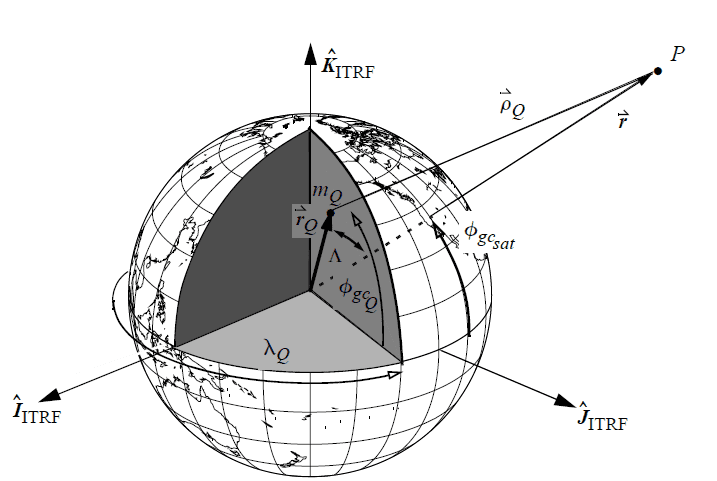
\includegraphics[width=0.75\linewidth]{Resimler/Earth Gravitational Potential.png}
  \caption{Dünya içindeki bir kütle elemanı $m_Q$ (konumu $\mathbf r_Q$) ile dış uzaydaki gözlem noktası $P$ (konumu $\mathbf r$) arasındaki geometri.}
  \label{fig:earth_potential_geometry}
\end{figure}

Şekil~\ref{fig:earth_potential_geometry}’de görülen $\Lambda$ açısı,
$\mathbf r$ ile $\mathbf r_Q$ doğrultuları arasındaki açıdır.
Kosinüs teoremi kullanılarak iki nokta arasındaki uzaklık
\begin{equation}
\rho_Q^{\,2}
=
r^2+r_Q^2-2rr_Q\cos\Lambda
\label{eq:rhoQ_coslaw_here}
\end{equation}
şeklinde elde edilir.
Dış uzaydaki bir gözlem noktası için genellikle $r>r_Q$ olduğundan
\begin{equation}
\alpha=\frac{r_Q}{r}
\qquad (0\le \alpha<1)
\label{eq:alpha_def_here}
\end{equation}
oranı tanımlanır.
Böylece \eqref{eq:rhoQ_coslaw_here} ifadesi
\begin{equation}
\rho_Q
=
r\sqrt{1-2\alpha\cos\Lambda+\alpha^2}
\label{eq:rhoQ_alpha_here}
\end{equation}
biçimine indirgenir ve integrand
\begin{equation}
\frac{1}{\rho_Q}
=
\frac{1}{r}\,
\frac{1}{\sqrt{1-2\alpha\cos\Lambda+\alpha^2}}
\label{eq:inv_rhoQ_factor}
\end{equation}
haline gelir.


Legendre \eqref{eq:inv_rhoQ_factor} ifadesinde hem $r$ hem $r_Q$ (yani $\alpha$), hem de açıya bağlı $\cos\Lambda$ aynı karekökün içinde birbirine karıştığını fark etmişti. Bu şekilde integrali doğrudan almak çoğu zaman çok zor olduğundan doğrudan integral almak yerine ne yapabilirim diye düşündü. Bunun üzerine integraldeki $1/\rho_Q$ ifadesini, $r$ ve $r_Q$ birbirinden ayrılmış şekilde bir seri haline getirip integralini alabileceğini farketti.

\medskip
 $\alpha=r_Q/r<1$ olduğundan \eqref{eq:inv_rhoQ_factor} içindeki
\(\bigl(1-2\alpha\cos\Lambda+\alpha^2\bigr)^{-1/2}\) ifadesini
$\alpha$ cinsinden bir seri olarak açmak mümkündür.
Legendre, Taylor açılımının atası sayılan Newton binom açılımını
bu tür ifadeler üzerinde kullanıp terimleri düzenlediğinde,
$\alpha$ kuvvetlerinin katsayılarının sadece açıya bağlı kaldığını, hatta bunun $\cos\Lambda$ cinsinden bir polinom ailesi oluşturduğunu görür. Bu polinomları sistematik biçimde tanımlamak için de \textbf{}{üretici fonksiyon} (\emph{generating function}) fikrini ortaya koyar.

\medskip
\noindent
\textbf{Newton binom açılımı:}
Dış bölgede $\alpha<1$ olduğundan, şu ifadeyi $\alpha$ cinsinden seri açabiliriz:
\begin{equation}
\frac{1}{\sqrt{1-2\alpha\cos\Lambda+\alpha^2}}
=
\left(1+u\right)^{-1/2},
\qquad
u:=\alpha^2-2\alpha\cos\Lambda.
\label{eq:u_def}
\end{equation}
Genelleştirilmiş Newton binom açılımı
\begin{equation}
(1+u)^{-1/2}
=
1-\frac{1}{2}u+\frac{3}{8}u^2-\frac{5}{16}u^3+\mathcal{O}(u^4)
\label{eq:newton_binom_series}
\end{equation}
şeklindedir.
Şimdi $u=\alpha^2-2\alpha\cos\Lambda$ yerine koyup,
$\alpha$ mertebelerine göre terimleri toplayalım.

Önce $u$ ve kuvvetlerini $\alpha$ cinsinden açalım:
\begin{align}
u &= \alpha^2-2\alpha\cos\Lambda,\\[4pt]
u^2 &= (\alpha^2-2\alpha\cos\Lambda)^2
= \alpha^4 -4\alpha^3\cos\Lambda +4\alpha^2\cos^2\Lambda,\\[4pt]
u^3 &= (\alpha^2-2\alpha\cos\Lambda)^3
= \alpha^6 -6\alpha^5\cos\Lambda +12\alpha^4\cos^2\Lambda -8\alpha^3\cos^3\Lambda.
\end{align}

Bunları \eqref{eq:newton_binom_series} içine koyup
$\alpha^3$ mertebesine kadar (yani $\mathcal{O}(\alpha^4)$’e kadar ihmal ederek)
toplayalım.

\paragraph{1) $-\tfrac12 u$ katkısı:}
\begin{equation}
-\frac12 u
=
-\frac12(\alpha^2-2\alpha\cos\Lambda)
=
\alpha\cos\Lambda-\frac12\alpha^2.
\end{equation}

\paragraph{2) $\tfrac{3}{8}u^2$ katkısı:}
$\alpha^3$’e kadar sadece $\alpha^2$ ve $\alpha^3$ terimleri gerekli:
\begin{equation}
\frac{3}{8}u^2
=
\frac{3}{8}\left(4\alpha^2\cos^2\Lambda -4\alpha^3\cos\Lambda + \alpha^4\right)
=
\frac{3}{2}\alpha^2\cos^2\Lambda
-\frac{3}{2}\alpha^3\cos\Lambda
+\mathcal{O}(\alpha^4).
\end{equation}

\paragraph{3) $-\tfrac{5}{16}u^3$ katkısı:}
$\alpha^3$ mertebesine kadar yalnızca $-8\alpha^3\cos^3\Lambda$ terimi önemlidir:
\begin{equation}
-\frac{5}{16}u^3
=
-\frac{5}{16}\left(-8\alpha^3\cos^3\Lambda+\mathcal{O}(\alpha^4)\right)
=
\frac{5}{2}\alpha^3\cos^3\Lambda
+\mathcal{O}(\alpha^4).
\end{equation}

\paragraph{4) Tüm katkıların toplanması.}
Şimdi tüm parçaları bir araya getirirsek:
\begin{align}
\frac{1}{\sqrt{1-2\alpha\cos\Lambda+\alpha^2}}
&=
1
+\left(\alpha\cos\Lambda\right) \nonumber\\
&\quad
+\alpha^2\left(\frac{3}{2}\cos^2\Lambda-\frac{1}{2}\right)\nonumber\\
&\quad
+\alpha^3\left(\frac{5}{2}\cos^3\Lambda-\frac{3}{2}\cos\Lambda\right)
+\mathcal{O}(\alpha^4).
\label{eq:explicit_series_alpha}
\end{align}

Bu sonuç çok önemli bir şeyi açıkça gösterir:
$\alpha$ kuvvetlerinin katsayıları,
sadece $\cos\Lambda$'ya bağlı \textbf{polinomlar}dır.
Gerçekten de
\begin{align}
P_0[\cos\Lambda]&=1,\\
P_1[\cos\Lambda]&=\cos\Lambda,\\
P_2[\cos\Lambda]&=\frac12\left(3\cos^2\Lambda-1\right),\\
P_3[\cos\Lambda]&=\frac12\left(5\cos^3\Lambda-3\cos\Lambda\right),
\end{align}
olduğundan \eqref{eq:explicit_series_alpha} ifadesi,
Legendre polinomlarının ürettiği seriyle birebir örtüşür:
\begin{equation}
\frac{1}{\sqrt{1-2\alpha\cos\Lambda+\alpha^2}}
=
\sum_{n=0}^{\infty}P_n[\cos\Lambda]\,\alpha^n,
\qquad (0\le \alpha<1).
\end{equation}


Denklemde $\cos\Lambda \Rightarrow x, \qquad \alpha \Rightarrow \frac{r_Q}{r}$ yazıldığında \eqref{eq:inv_rhoQ_factor} doğrudan seri açılır:
\begin{equation}
\frac{1}{\rho_Q}
=
\frac{1}{r}
\sum_{n=0}^{\infty}
P_n[\cos\Lambda]\,\alpha^n
=
\frac{1}{r}
\sum_{n=0}^{\infty}
P_n[x]\left(\frac{r_Q}{r}\right)^n,
\qquad (r>r_Q).
\label{eq:1_over_rhoQ_legendre}
\end{equation}
Buradaki $P_n(\cdot)$ polinomları,
bugün \textbf{Legendre polinomları} olarak bildiğimiz polinom ailesidir.

Resimde görüldüğü üzere ilk 6 Legendre polinomu,
$[-1,1]$ aralığında çizdirilmiştir.

\begin{figure}[h]
    \centering
    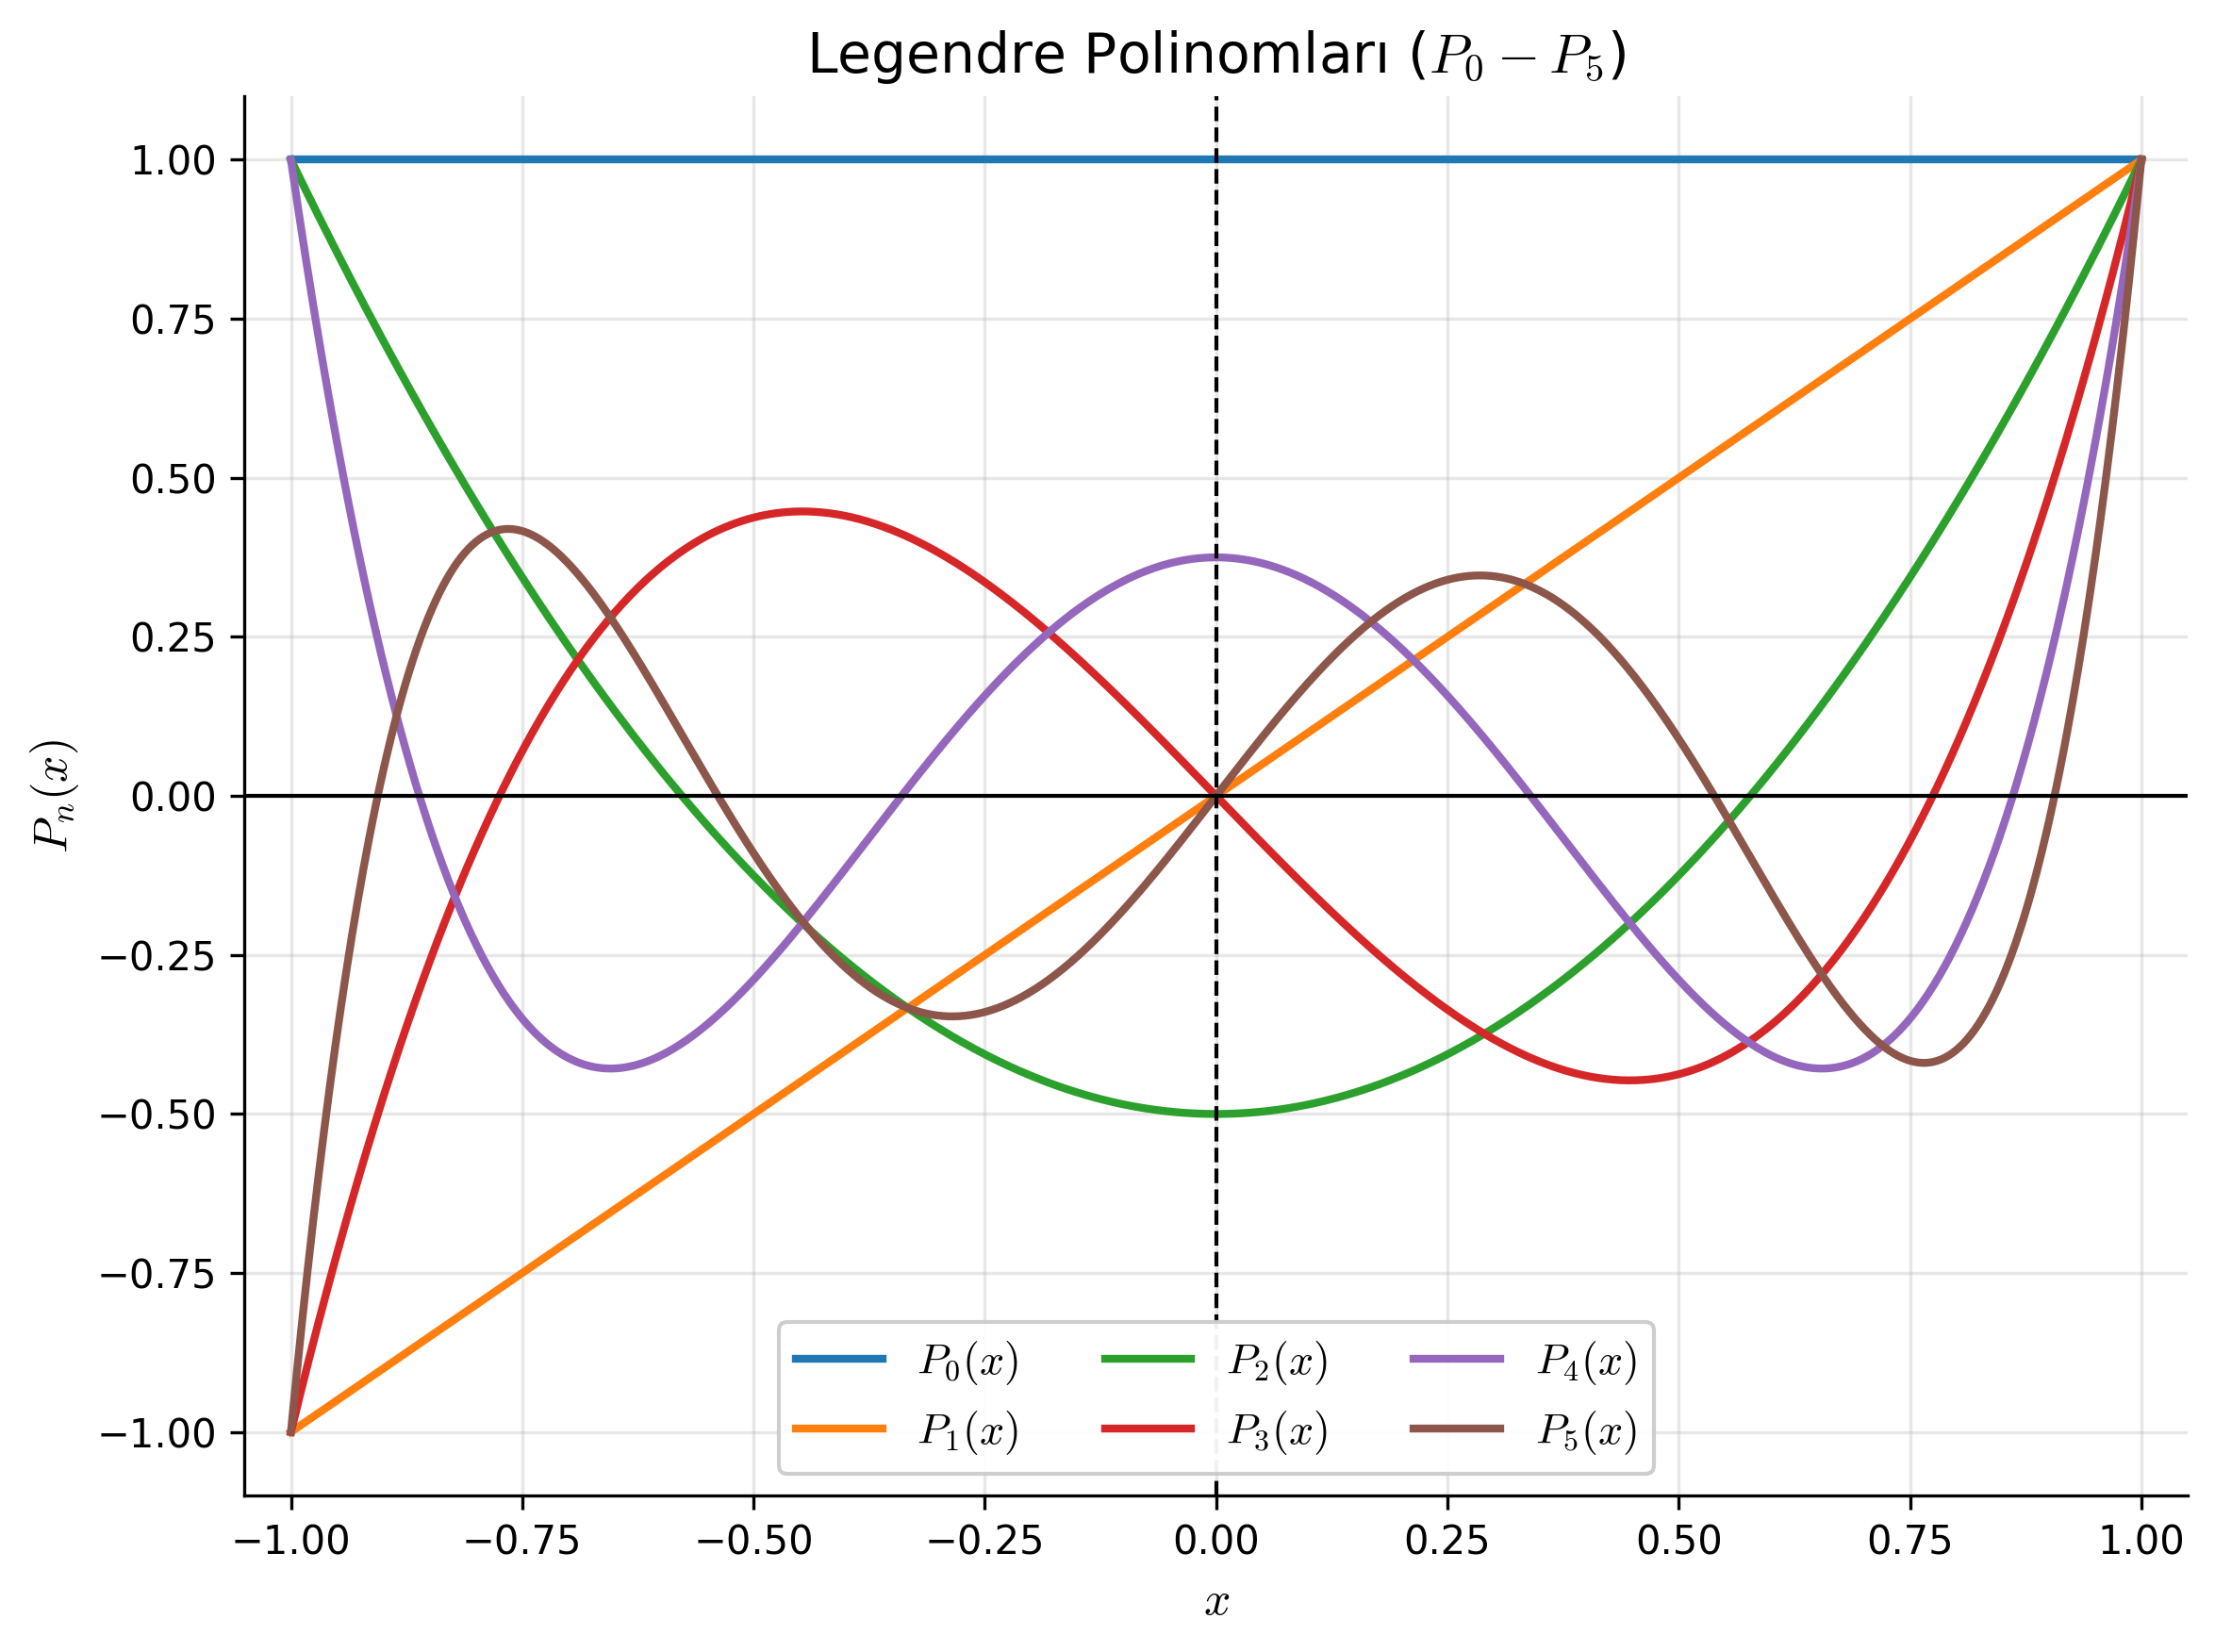
\includegraphics[width=0.6\linewidth]{Resimler/Poly First 6.png}
    \caption{$[-1,1]$ aralığında ilk 6 Legendre polinomu ($P_0$--$P_5$).}
    \label{fig:Legendre_poly_first6}
\end{figure}



\newpage
\subsection{Legendre'den Sonra}

Legendre’in potansiyel probleminden hareketle tanımladığı bu polinomlar, zamanla matematiksel açıdan da büyük önem kazandı.
Özellikle 19. yüzyılda, Legendre polinomlarının farklı yollarla yeniden üretilebildiği ve bu polinomlar için pratik kapalı ifadeler yazılabildiği gösterildi. Bunların en kullanışlı örneklerinden biri, \textbf{Olinde Rodrigues}’in 1816’da verdiği üretim formülüdür. Legendre’in yaklaşımından birkaç on yıl sonra ortaya çıkan bu sonuç, $P_n(x)$ polinomlarını doğrudan üretmek için güçlü bir kısa yol sağlar.

% ------------------------------------------------------------
\subsubsection{Rodrigues Formülü}

Legendre polinomlarının en bilinen kapalı üretim ifadelerinden biri Rodrigues formülüdür:
\begin{equation}
P_n(x)=\frac{1}{2^n n!}\frac{d^n}{dx^n}\Big[(x^2-1)^n\Big].
\label{eq:Rodrigues}
\end{equation}

Bu formül iki noktayı aynı anda netleştirir:
(i) $P_n(x)$ gerçekten bir polinomdur,
(ii) derecesi de tam olarak $n$’dir.
Çünkü $(x^2-1)^n$ ifadesi binom açılımı ile sonlu sayıda terime ayrılır:
\[
(x^2-1)^n
= \sum_{k=0}^{n}\binom{n}{k}(x^2)^{\,n-k}(-1)^k
= \sum_{k=0}^{n}\binom{n}{k}(-1)^k x^{2(n-k)}.
\]
Bu polinomun en yüksek derecesi $2n$’dir.
$n$ kez türev alındığında derecesi $2n-n=n$ olur ve sonuç yine polinom kalır.
Dolayısıyla $P_n$ notasyonu, polinomun derecesiyle doğrudan uyumludur.

% ------------------------------------------------------------
\subsubsection{Rodrigues ile İlk 10 Legendre Polinomu}

Rodrigues formülü \eqref{eq:Rodrigues} kullanılarak $P_n(x)$ polinomları
tek tek üretilebilir. Aşağıda $n=0$ ile $n=9$ arasındaki ilk 10 Legendre polinomu
tablo halinde verilmiştir.

\begin{table}[h]
\centering
\renewcommand{\arraystretch}{1.5}
\setlength{\tabcolsep}{12pt}
\begin{tabular}{c l c l}
\toprule
\textbf{$n$} & \textbf{$P_n(x)$} & \textbf{$n$} & \textbf{$P_n(x)$} \\
\midrule
0 & $1$
& 5 & $\frac{1}{8}\,(63x^5-70x^3+15x)$ \\[6pt]

1 & $x$
& 6 & $\frac{1}{16}\,(231x^6-315x^4+105x^2-5)$ \\[6pt]

2 & $\frac{1}{2}\,(3x^2-1)$
& 7 & $\frac{1}{16}\,(429x^7-693x^5+315x^3-35x)$ \\[6pt]

3 & $\frac{1}{2}\,(5x^3-3x)$
& 8 & $\frac{1}{128}\,(6435x^8-12012x^6+6930x^4-1260x^2+35)$ \\[8pt]

4 & $\frac{1}{8}\,(35x^4-30x^2+3)$
& 9 & $\frac{1}{128}\,(12155x^9-25740x^7+18018x^5-4620x^3+315x)$ \\
\bottomrule
\end{tabular}
\caption{Rodrigues formülü ile üretilen ilk 10 Legendre polinomu ($P_0$--$P_9$).}
\label{tab:first10_legendre}
\end{table}



% ========== Ek Okuma ve Alternatif Yaklaşımlar ===========
\newpage
\section{Ek Okuma ve Teorik Arkaplan}
\label{subsec:ek_okuma_alternatifler}

Rodrigues formülü, Legendre polinomlarını üretmek için son derece pratik bir araçtır. Ancak bu polinomların nereden çıktığını ve diğer ortogonal polinom aileleriyle nasıl ilişkilendiğini bilmek, özellikle mühendislikte \uline{doğru probleme doğru baz} seçebilmek açısından önemlidir. Bu alt bölümde, Legendre polinomlarının diferansiyel denklem kökeni, cebirsel inşası ve alternatif ortogonal bazlarla ilişkisi özetlenmektedir.

% ------------------------------------------------------------
\subsection{Diferansiyel Denklem Kökeni ve Sturm--Liouville}

Legendre polinomları, küresel simetri içeren problemlerde (özellikle Laplace denklemi)
değişkenlerin ayrılması uygulanınca doğal olarak ortaya çıkan Legendre diferansiyel denkleminin çözümleridir:
\begin{equation}
(1-x^2)\,y''-2x\,y' + n(n+1)\,y = 0.
\label{eq:legendre_de_bg}
\end{equation}
Bu denklem Sturm--Liouville formuna da yazılabilir:
\begin{equation}
\frac{d}{dx}\!\left[(1-x^2)\,y'\right] + n(n+1)\,y = 0,
\qquad x\in[-1,1].
\label{eq:legendre_sl_form}
\end{equation}


Pek çok fiziksel problem (titreşim modları, ısı iletimi, potansiyel problemleri vb.) uygun sınır koşulları altında bir \textbf{özdeğer problemi}ne indirgenir ve bu problemler çoğunlukla

\begin{equation}
\frac{d}{dx}\!\left[p(x)\,y'\right] + \bigl[\lambda\,w(x)-q(x)\bigr]\,y = 0,
\qquad w(x)>0
\label{eq:sl_general}
\end{equation}

şeklinde yazılabilir. Buradaki kritik nokta, çözüm ailesinin doğal olarak bir \textbf{ağırlık fonksiyonu} $w(x)$ ile birlikte gelmesidir.

Sturm--Liouville teorisi gereğince, \eqref{eq:sl_general} biçimindeki bir özdeğer probleminde
farklı özdeğerlere karşılık gelen özfonksiyonlar,
\begin{equation}
\int_{-1}^{1} y_n(x)\,y_m(x)\,w(x)\,dx = 0 \qquad (n\neq m)
\label{eq:sl_ortho_general}
\end{equation}
anlamında \textbf{ağırlıklı} ortogonaldir.

Legendre durumunda \eqref{eq:legendre_sl_form} ile karşılaştırınca
$p(x)=1-x^2$, $q(x)=0$, $\lambda=n(n+1)$ ve en önemlisi $w(x)=1$ elde edilir.
Dolayısıyla ortogonallik, klasik (ağırlıksız) biçime indirgenir:

\begin{equation}
\int_{-1}^{1} P_n(x)\,P_m(x)\,dx = 0 \qquad (n\neq m).
\label{eq:legendre_ortho_bg}
\end{equation}

Burada dikkat edilmesi gereken nokta şudur:
\eqref{eq:legendre_de_bg} denkleminin ikinci bağımsız çözümü (Legendre $Q_n$) uç noktalar civarında tekil davranır; fiziksel uygulamalarda genellikle düzenli kalan $P_n$ ailesi seçilir.

% ------------------------------------------------------------
\newpage
\subsection{Gram--Schmidt Ortogonalleştirmesi}

Legendre polinomları lineer cebir perspektifiyle de inşa edilebilir. Bu yaklaşımın ana fikri ``Ortogonal polinom ailesi'' seçiminin, hangi iç-çarpımı (dolayısıyla hangi ağırlığı) kullandığına bağlı olmasındadır.

Genel olarak $[-1,1]$ üzerinde bir \textbf{ağırlıklı} iç-çarpım tanımlayalım:
\begin{equation}
\langle f,g\rangle_w=\int_{-1}^{1} f(x)\,g(x)\,w(x)\,dx,
\qquad w(x)>0.
\label{eq:weighted_inner_bg}
\end{equation}
Bu durumda Gram--Schmidt sürecini standart monom bazına
$\{1,x,x^2,\ldots\}$ uygularsan, elde ettiğin ortogonal polinom ailesi
\emph{seçtiğin} $w(x)$ ağırlığına göre şekillenir.

Klasik Legendre ailesi için özel seçim $w(x)=1$'dir; bu seçim \eqref{eq:weighted_inner_bg}'yi
alışıldık $L^2([-1,1])$ iç-çarpımına indirger:
\begin{equation}
\langle f,g\rangle=\int_{-1}^{1} f(x)\,g(x)\,dx.
\label{eq:L2_inner_bg}
\end{equation}
Dolayısıyla $w(x)=1$ altında Gram--Schmidt uygulanınca,
uygun normalizasyonla elde edilen ortogonal polinom ailesi Legendre polinomlarıdır.

Bu bakış, ortogonalliği ``tanımsal'' olarak değil,
doğrudan bir ortogonalleştirme sürecinin sonucu olarak görmeyi sağlar.
Ayrıca, farklı $w(x)$ seçimlerinin farklı aileleri (ör.\ Chebyshev, Jacobi, Gegenbauer vb.)
doğurduğu fikrini de doğal biçimde verir.

% ------------------------------------------------------------
\subsection{Diğer Ortogonal Polinom Aileleri ve Ağırlık Fonksiyonu}

İç çarpımın tanım aralığı ve ağırlık fonksiyonu $w(x)$ değiştirildiğinde,
farklı fiziksel problemlere daha iyi uyan farklı ortogonal polinom aileleri elde edilir.
Genel çerçeve:
\[
\langle f,g\rangle_w=\int_a^b f(x)\,g(x)\,w(x)\,dx, \qquad w(x)>0.
\]
Aşağıdaki aileler, Legendre ile aynı ``sabit aralık'' ($[-1,1]$) bağlamında özellikle sık karşılaşılan örneklerdir:
\begin{itemize}
    \item \textbf{Chebyshev polinomları ($T_n$):}
    $[-1,1]$ aralığında $w(x)=(1-x^2)^{-1/2}$ ağırlığıyla ortogonaldir.
    Sayısal açıdan iki pratik avantajı öne çıkar:
    (i) düğümler uçlara doğru kümelendiği için uç davranışlarını iyi yakalar,
    (ii) kosinüs dönüşümü (FFT-türevi) ile katsayı hesapları çok hızlı yapılabilir.
    Bu nedenle spektral yöntemlerde ve interpolasyonda sıklıkla tercih edilir.

    \item \textbf{Jacobi polinomları ($P_n^{(\alpha,\beta)}$):}
    $[-1,1]$ aralığında
    \[
      w(x)=(1-x)^{\alpha}(1+x)^{\beta}, \qquad \alpha,\beta>-1
    \]
    ağırlığıyla ortogonaldir.
    Bu aile, uç noktalar yakınındaki davranışı ``ayar'' edebilmesiyle önemlidir:
    çözümün $x=\pm 1$ civarında belirgin asimetrisi, sınır tabakası benzeri yoğunluğu
    veya ağırlıklı hata ölçütü varsa $\alpha,\beta$ seçimi ile temsil kalitesi artabilir.
    Ayrıca \emph{Legendre} ($\alpha=\beta=0$) ve \emph{Chebyshev} (uygun $\alpha,\beta$ seçimleri) bu ailenin özel durumlarıdır.

    \item \textbf{Gegenbauer / ultrasferik polinomlar ($C_n^{(\lambda)}$):}
    $[-1,1]$ aralığında
    \[
      w(x)=(1-x^2)^{\lambda-\tfrac12}, \qquad \lambda>-1/2
    \]
    ağırlığıyla ortogonaldir.
    Daha yüksek boyutlu küresel simetriye sahip problemlerde (``$d$-boyutlu küre'' genellemeleri)
    doğal olarak ortaya çıkar; bu yüzden küresel harmonik genişletmelerinin arka planında
    sıkça karşımıza çıkar.

    \item \textbf{İlişkili Legendre fonksiyonları ($P_\ell^m$):}
    Tek değişkenli bir ``aile'' gibi düşünülebilir: küresel harmoniklerin açısal parçasını oluşturur.
    Sabit $m$ için $x=\cos\theta$ değişkeninde $[-1,1]$ üzerinde ortogonallik korunur
    (normalizasyon katsayıları farklıdır).
    Bu nedenle Laplace denklemi / potansiyel problemleri bağlamında Legendre'nin en yakın akrabasıdır.
\end{itemize}

\noindent (Not: $[0,\infty)$ veya $(-\infty,\infty)$ gibi sonsuz aralıklarda çalışılan problemlerde
Laguerre/Hermite aileleri daha doğal olur; ancak bu metnin odağı sabit aralık ve küresel simetri olduğu için
yukarıdaki aileler daha doğrudan bağlantılıdır.)

% ------------------------------------------------------------
\subsection{Neden Legendre?}

Bir simülasyon veya yaklaşım probleminde baz fonksiyonu seçerken,
bazın (i) problemin geometrisiyle uyumu, (ii) sınır koşullarıyla uyumu,
(iii) yakınsaklık davranışı ve (iv) hata ölçütüyle ilişkisi birlikte değerlendirilir.
Bu çerçevede Legendre tabanı, birçok mühendislik probleminde güçlü bir adaydır:

\begin{enumerate}
    \item \textbf{Periyodiklik ve sınır koşulları (Fourier vs.\ polinom bazlar):}
    Fourier serileri periyodik problemlerde idealdir ve boylam gibi periyodik değişkenlerde zaten kaçınılmazdır.
    Buna karşın sabit aralıkta, periyodik olmayan ve belirli sınır davranışı istenen problemlerde
    polinom bazlı temsiller (Legendre/Chebyshev/Jacobi gibi) daha esnek ve hızlı yakınsak olabilir.
    (Not: Gibbs fenomeni esasen süreksizliklerde belirgindir; periyodik olmayan uzatmalar da benzer dalgalanmayı tetikleyebilir.)

    \item \textbf{Hata ölçütü ve fiziksel anlam (Chebyshev/Jacobi vs.\ Legendre):}
    Chebyshev polinomları çoğu zaman maksimum hatayı baskılamaya yönelik pratik avantajlar sunar
    ve uçlara yakın bölgelerde daha fazla ``örnekleme'' yapar.
    Jacobi ailesi ise uç davranışını $\alpha,\beta$ ile ağırlıklandırarak probleme özel ayar yapmayı mümkün kılar.
    Legendre polinomları ise $w(x)=1$ altında $L_2([-1,1])$ anlamında ortogonal oldukları için
    katsayılar doğrudan ortogonal projeksiyonla ayrılır;
    hata ``enerjisi'' doğal biçimde $L_2$ normu üzerinden yorumlanır.
    Enerji prensipleriyle ifade edilen birçok mekanik ve alan probleminde bu yorumlama daha doğrudan ve rahattır.

    \item \textbf{İntegral hesapları ve Gauss--Legendre kuadraturu:}
    Legendre tabanı, Gauss--Legendre noktalarıyla birlikte kullanıldığında
    polinom integrallerini çok yüksek doğrulukla (ve belirli dereceye kadar tam) hesaplamayı sağlar.
    Bu, Galerkin / spektral eleman türü yöntemlerde
    matris elemanlarının (kütle/rijitlik) sayısal olarak verimli ve güvenilir biçimde kurulmasına yardım eder.

    \item \textbf{Küresel simetriyle yakın akrabalık:}
    Potansiyel problemleri ve küresel harmonikler bağlamında
    açısal değişken $x=\cos\theta$ üzerinden Legendre ve ilişkili Legendre yapıları zaten doğal biçimde ortaya çıkar.
    Bu yüzden ``baz seçimi'' çoğu zaman ekstra bir tercih değil, problemin geometrisinin dayattığı doğal sonuçtur.
\end{enumerate}



% ======================= Deneme Bölgesi ======================


% =============== Küresel Harmonikler =================
\newpage
\section{Küresel Harmonikler}

Önceki bölümde incelenen Legendre polinomları ($P_n$), kütle dağılımının dönel eksene göre simetrik olduğu (boylamdan bağımsız) idealize edilmiş durumları modellemek için temel teşkil eder. Ancak Dünya gibi gerçek gökcisimleri, gerek yüzey topoğrafyaları (örneğin sıradağlar ve okyanus çukurları)
gerekse iç yoğunluk düzensizlikleri nedeniyle küresel veya eksenel simetriden saparlar. Bu kütle anomalileri, yerçekimi potansiyelinin sadece enleme göre değil, boylam ($\lambda$) yönünde de değişmesine neden olur. Dolayısıyla, gezegenin çekim alanını yüksek hassasiyetle modelleyebilmek için,
Legendre polinomlarının boylamı da içerecek şekilde genelleştirilmesi gerekmektedir. Bu bölümde, potansiyel teorisinin temeli olan Laplace denklemi küresel koordinatlarda ele alınarak, küre yüzeyi üzerindeki herhangi bir skaler alanın spektral olarak ifade edilmesini sağlayan ve \textbf{Küresel Harmonikler} olarak adlandırılan ortogonal baz fonksiyonları seti türetilecektir. 

\textbf{Notasyon:} Bu noktadan itibaren jeodezi literatüründeki yaygın kullanıma uygun olarak derece indisi $n$ yerine $\ell$ kullanılacak; dolayısıyla $P_n(\cdot)$ gösterimi $P_\ell(\cdot)$ biçiminde yazılacaktır.

% ------------------------------------------------------------
\subsection{Laplace Denklemi ve Küresel Harmonik Bazı}
\label{subsec:laplace_sep_sphharm}

Yerçekimi, elektrostatik ve benzeri alan teorilerinde temel nicelik,
bir skaler potansiyel fonksiyonu $U(\mathbf{r})$’dir.
Kaynak içermeyen bölgelerde (kütle ya da yük olmayan hacimlerde) potansiyel
\textbf{Laplace denklemini} sağlar:
\begin{equation}
\nabla^2 U = 0 .
\label{eq:laplace}
\end{equation}
\noindent

\subsubsection{Küresel Koordinatlarda Laplace Operatörü}

Problemimiz merkezi bir cisim (ör.\ Dünya) etrafında tanımlandığı için küresel koordinatlar seçilebilecek en uygun koordinatlardır:
\[
(r,\theta,\lambda),
\]
burada $r$ merkezden uzaklık, $\theta$ \textbf{kolatitude} (kuzey kutbundan ölçülen açı), $\lambda$ ise \textbf{boylam}dır.
İleride geodezik notasyona geçiş için ayrıca \textbf{geocentric latitude} $\phi_{gc}$ tanımlarsak
\begin{equation}
\phi_{gc}=\frac{\pi}{2}-\theta
\quad\Longrightarrow\quad
\sin\phi_{gc}=\cos\theta,\qquad \cos\phi_{gc}=\sin\theta.
\label{eq:theta_phi_relation}
\end{equation}

Laplace denklemi küresel koordinatlarda
\begin{equation}
\nabla^2 U =
\frac{1}{r^2}\frac{\partial}{\partial r}
\left(r^2\frac{\partial U}{\partial r}\right)
+
\frac{1}{r^2\sin\theta}\frac{\partial}{\partial\theta}
\left(\sin\theta\frac{\partial U}{\partial\theta}\right)
+
\frac{1}{r^2\sin^2\theta}
\frac{\partial^2 U}{\partial\lambda^2}
= 0 .
\label{eq:laplacian_spherical}
\end{equation}
Burada $r$, $\theta$ ve $\lambda$ bağımlılıkları birbirine karışmış durumdadır;
bu tür PDE’ler için en sistematik çıkış yolu \textbf{değişkenlere ayırma}dır.

\subsubsection{Değişkenlere Ayırma Varsayımı}

Denklem lineer ve homojen yapıdadır. Değişkenlerin ayrılması yöntemi uygulanarak çözüm şu şekilde önerilirse:
\begin{equation}
U(r,\theta,\lambda) = R(r)\,\Theta(\theta)\,\Phi(\lambda).
\label{eq:separation_ansatz}
\end{equation}

\noindent
\eqref{eq:separation_ansatz} ifadesini \eqref{eq:laplacian_spherical} içine yerleştirince türevler şu şekilde açılır:
\begin{align}
\frac{\partial U}{\partial r} &= \Theta(\theta)\,\Phi(\lambda)\,\frac{dR}{dr},
&
\frac{\partial U}{\partial \theta} &= R(r)\,\Phi(\lambda)\,\frac{d\Theta}{d\theta},
&
\frac{\partial^2 U}{\partial \lambda^2} &= R(r)\,\Theta(\theta)\,\frac{d^2\Phi}{d\lambda^2}.
\label{eq:partials_sep}
\end{align}
Bunları \eqref{eq:laplacian_spherical}'de yerine koyarsak
\begin{equation}
\frac{\Theta\,\Phi}{r^2}\frac{d}{dr}\!\left(r^2\frac{dR}{dr}\right)
+
\frac{R\,\Phi}{r^2\sin\theta}\frac{d}{d\theta}\!\left(\sin\theta\frac{d\Theta}{d\theta}\right)
+
\frac{R\,\Theta}{r^2\sin^2\theta}\frac{d^2\Phi}{d\lambda^2}
=0
\label{eq:after_factor_out}
\end{equation}
elde edilir.

\noindent
Son olarak tüm denklemi $R(r)\,\Theta(\theta)\,\Phi(\lambda)$ ile bölersek
\begin{equation}
\frac{1}{R}\frac{d}{dr}\!\left(r^2\frac{dR}{dr}\right)
+
\frac{1}{\Theta\sin\theta}\frac{d}{d\theta}\!\left(\sin\theta\frac{d\Theta}{d\theta}\right)
+
\frac{1}{\Phi\sin^2\theta}\frac{d^2\Phi}{d\lambda^2}
=0
\label{eq:separated_pre}
\end{equation}
elde edilir.
Her terim farklı bir değişkene bağlı olduğundan bu toplamın her noktada sıfır olabilmesi,
terimlerin uygun \textbf{ayırma sabitleri} ile ayrılmasını zorunlu kılar.

% ------------------ Boylam Denklemi -----------------
\subsubsection{Boylam Denklemi, Tek-Değerlilik ve Periyodiklik}
\label{subsubsec:lambda_periodicity}

\eqref{eq:separated_pre} denkleminde yalnızca $\lambda$'ya bağlı terim
$\frac{1}{\Phi}\frac{d^2\Phi}{d\lambda^2}$ ifadesidir. Değişkenlerin ayrılabilmesi için
\begin{equation}
\frac{1}{\Phi}\frac{d^2\Phi}{d\lambda^2}=-m^2
\label{eq:lambda_eq}
\end{equation}
seçilir. Buradaki eksi işareti, çözümlerin salınımlı olmasını sağlar. Ayrıca potansiyelin tek-değerli olması gerekir:
\begin{equation}
U(r,\theta,\lambda)=U(r,\theta,\lambda+2\pi)
\quad\Longrightarrow\quad
\Phi(\lambda)=\Phi(\lambda+2\pi),
\label{eq:single_valuedness}
\end{equation}
bu şart $e^{im\lambda}$ temsili için $m\in\mathbb{Z}$ tamsayılığını zorunlu kılar. Dolayısıyla
\eqref{eq:lambda_eq} denkleminin çözümleri
\begin{equation}
\Phi(\lambda)=e^{\pm i m\lambda},
\qquad m\in\mathbb{Z}
\label{eq:lambda_solution_complex}
\end{equation}
ya da eşdeğer gerçek biçimde
\begin{equation}
\Phi(\lambda)=
\begin{cases}
\cos(m\lambda),\\[2pt]
\sin(m\lambda),
\end{cases}
\qquad m=0,1,2,\dots
\label{eq:lambda_solution_real}
\end{equation}
şeklindedir. Gerçek baz ($\sin/\cos$) kullanıldığında negatif $m$ değerleri aynı fonksiyon uzayını yeniden ürettiğinden,
çoğunlukla $m\ge 0$ ile yetinilir.

\subsubsection{Radyal ve Kolatitude Denklemlerinin Ayrılması}
\label{subsubsec:radial_theta_split}

\eqref{eq:lambda_eq} seçimi \eqref{eq:separated_pre} içine yerleştirildiğinde,
$r$-bağımlı terim ile $\theta$-bağımlı terim birbirinden ayrılabilir. Burada boylam sembolü $\lambda$ ile karışmaması için
ayırma sabiti (özdeğer) \textbf{$\nu$} ile gösterilsin:
\begin{align}
\frac{1}{R}\frac{d}{dr}\!\left(r^2\frac{dR}{dr}\right) &= \nu,
\label{eq:radial_eq_general}\\[4pt]
\frac{1}{\sin\theta}\frac{d}{d\theta}
\left(\sin\theta\frac{d\Theta}{d\theta}\right)
-
\frac{m^2}{\sin^2\theta}\,\Theta
&=
-\nu\,\Theta.
\label{eq:theta_eq_theta}
\end{align}
Böylece açısal problem $\nu$ özdeğerini belirler; radyal problem ise bu özdeğere karşılık gelen $r$-bağımlılığını verir.

\subsubsection{Kolatitude Denklemi: $x=\cos\theta$ Dönüşümü ve Associated Legendre}
\label{subsubsec:theta_associated_legendre}

Bu noktada $\theta\in[0,\pi]$ aralığını $[-1,1]$ aralığına taşıyan standart dönüşüm
\begin{equation}
x=\cos\theta
\label{eq:x_costheta}
\end{equation}
seçilir. Böylece $\sin^2\theta=1-x^2$ olur ve ayrıca küre üzerindeki doğal ölçü
$dA=\sin\theta\,d\theta\,d\lambda$ nedeniyle
\begin{equation}
dx=-\sin\theta\,d\theta
\quad\Longrightarrow\quad
\int_{0}^{\pi}(\cdot)\,\sin\theta\,d\theta
=
\int_{-1}^{1}(\cdot)\,dx
\label{eq:measure_transform}
\end{equation}
ilişkisi elde edilir.

\medskip
\noindent
$\Theta(\theta)$ fonksiyonunu $x$ cinsinden $y(x)\equiv \Theta(\theta(x))$ olarak tanımlayalım.
Zincir kuralıyla
\begin{equation}
\frac{d}{d\theta}
=
\frac{dx}{d\theta}\frac{d}{dx}
=
(-\sin\theta)\frac{d}{dx}
=
-\sqrt{1-x^2}\,\frac{d}{dx}
\label{eq:d_dtheta_to_d_dx}
\end{equation}
bulunur. Bu dönüşüm kullanıldığında, \eqref{eq:theta_eq_theta} içinde yer alan açısal operatör
\begin{equation}
\frac{1}{\sin\theta}\frac{d}{d\theta}\left(\sin\theta\frac{d\Theta}{d\theta}\right)
=
\frac{d}{dx}\left((1-x^2)\frac{dy}{dx}\right)
=
(1-x^2)\frac{d^2y}{dx^2}-2x\frac{dy}{dx}
\label{eq:legendre_operator}
\end{equation}
şeklinde $x$ değişkenine indirgenir. Son olarak $\sin^2\theta=1-x^2$ ifadesiyle birlikte
\eqref{eq:theta_eq_theta} denklemi
\begin{equation}
(1-x^2)\frac{d^2 y}{dx^2}
-2x\frac{dy}{dx}
+
\left[\nu-\frac{m^2}{1-x^2}\right]y
=0
\label{eq:associated_legendre_eq}
\end{equation}
biçimine dönüşür. Denklem \eqref{eq:associated_legendre_eq}, \textbf{associated Legendre
diferansiyel denklemi} olarak adlandırılır ve küresel harmonik bazın enlemsel
bileşenini belirleyen temel özdeğer problemidir.

\subsubsection{Düzenlilik Şartı ve Özdeğerlerin Kuantalanması}
\label{subsubsec:regularity_quantization}

\eqref{eq:associated_legendre_eq} diferansiyel denklemi, $x=\pm 1$ (yani $\theta=0,\pi$ kutupları)
noktasında \emph{tekil} bir yapı içerir; çünkü katsayılarda $(1-x^2)$ terimi yer almakta ve
$\frac{m^2}{1-x^2}$ ifadesi kutuplarda büyümeye eğilim göstermektedir. Yerçekimi potansiyeli gibi
fiziksel alanlar için kabul edilebilir çözümler, kutuplar civarında sonlu (düzenli) kalmalıdır.
Bu şart altında, genel çözümün kutuplarda diverge eden \emph{ikinci tür} bileşenleri (çoğu gösterimde $Q_\ell^m$)
elenir ve yalnızca düzenli sınıf (associated Legendre $P_\ell^m$) kabul edilir.

\medskip
\noindent
Bu \textbf{düzenlilik şartı}, \eqref{eq:associated_legendre_eq} denkleminin keyfi $\nu$ değerleri için değil,
yalnızca belirli ayrık özdeğerler için düzenli çözüme sahip olmasını zorunlu kılar. Buna göre özdeğer
\begin{equation}
\nu=\ell(\ell+1),
\qquad
\ell=0,1,2,\dots,
\qquad
|m|\le \ell
\label{eq:eigenvalues}
\end{equation}
biçiminde \textbf{kuantalanır} ve enlemsel çözümler
\begin{equation}
\Theta(\theta)=P_\ell^m[\cos\theta]
\label{eq:theta_solution_associated}
\end{equation}
şeklinde \textbf{associated Legendre} fonksiyonları ile ifade edilir. Burada $\ell$ dereceyi (degree),
$m$ ise mertebeyi (order) temsil eder; $|m|\le \ell$ koşulu, kutuplarda düzenlilik ile uyumlu çözüm sınıfını tanımlar.

% ------------------------------------------------------------
\subsubsection{Associated Legendre Fonksiyonlarının Açık İfadeleri ($\ell \le 4$)}
\label{subsubsec:explicit_legendre}

Teorik olarak tanımlanan $P_\ell^m[x]$ fonksiyonlarının fiziksel davranışını kavramak adına,
ilk dört dereceye ($\ell \le 4$) ait açık ifadeler Tablo \ref{tab:assoc_legendre_trig}'de sunulmuştur.
Fonksiyonların enlemle değişimini açıkça göstermek için değişken olarak $x$ yerine
doğrudan geocentric enlem ($\phi_{gc}$) kullanılmıştır.
Dönüşümde $x = \sin\phi_{gc}$ ve $(1-x^2)^{1/2} = \cos\phi_{gc}$ özdeşlikleri esas alınmıştır.

\begin{table}[h!]
    \centering
    \caption{İlk 4 derece için Normalize Edilmemiş (Conventional) Associated Legendre Fonksiyonları. Değişken: Geocentric Enlem ($\phi_{gc}$).}
    \renewcommand{\arraystretch}{1.8} % Formüllerin sıkışmaması için satır arasını biraz daha açtım
    \begin{tabular}{c c l}
        \hline
        \textbf{Derece ($\ell$)} & \textbf{Sıra ($m$)} & \textbf{Fonksiyon $P_{\ell,m}[\sin\phi_{gc}]$} \\
        \hline
        % --- Degree 0 ---
        0 & 0 & $1$ \\
        \hline
        % --- Degree 1 ---
        1 & 0 & $\sin\phi_{gc}$ \\
        1 & 1 & $\cos\phi_{gc}$ \\
        \hline
        % --- Degree 2 ---
        2 & 0 & $\frac{1}{2}(3\sin^2\phi_{gc} - 1)$ \\
        2 & 1 & $3\sin\phi_{gc}\cos\phi_{gc}$ \\
        2 & 2 & $3\cos^2\phi_{gc}$ \\
        \hline
        % --- Degree 3 ---
        3 & 0 & $\frac{1}{2}(5\sin^3\phi_{gc} - 3\sin\phi_{gc})$ \\
        3 & 1 & $\frac{3}{2}(5\sin^2\phi_{gc} - 1)\cos\phi_{gc}$ \\
        3 & 2 & $15\sin\phi_{gc}\cos^2\phi_{gc}$ \\
        3 & 3 & $15\cos^3\phi_{gc}$ \\
        \hline
        % --- Degree 4 ---
        4 & 0 & $\frac{1}{8}(35\sin^4\phi_{gc} - 30\sin^2\phi_{gc} + 3)$ \\
        4 & 1 & $\frac{5}{2}(7\sin^3\phi_{gc} - 3\sin\phi_{gc})\cos\phi_{gc}$ \\
        4 & 2 & $\frac{15}{2}(7\sin^2\phi_{gc} - 1)\cos^2\phi_{gc}$ \\
        4 & 3 & $105\sin\phi_{gc}\cos^3\phi_{gc}$ \\
        4 & 4 & $105\cos^4\phi_{gc}$ \\
        \hline
    \end{tabular}
    \label{tab:assoc_legendre_trig}
\end{table}

\noindent
\textbf{Not:} Tablodaki ifadeler, fonksiyonların kutuplarda ($\phi_{gc}=\pm 90^\circ$) ve
ekvatorda ($\phi_{gc}=0^\circ$) nasıl davrandığını açıkça gösterir. Örneğin $m=\ell$ (Sectoral)
durumlarında sadece $\cos\phi_{gc}$ terimlerinin bulunması, bu harmoniklerin ekvatorda maksimum genliğe ulaşıp
kutuplarda sıfırlandığını (kutup geçişli uydular için önemli bir detay) işaret eder.



% ---------- Rekürans Ve Pseudocode ------------
\subsection{Rekürans Bağıntıları ile Polinom}

Associated Legendre polinomları, Sturm--Liouville yapısı gereği zaten
ortogonal bir baz oluşturur. Bu nedenle teorik olarak Gram--Schmidt ile
sayısal ortogonalleştirme yapılabilse de, yüksek derecelerde bu yaklaşım
hem hesaplama maliyetini ciddi biçimde artırır (çok sayıda iç-çarpım gerektirir)
hem de sayısal kararlılık sorunlarına açık hâle gelebilir.
Bu yüzden pratik uygulamalarda $P_{\ell,m}$ değerleri doğrudan
rekürans bağıntıları ile üretilir.

Bu çalışmada, jeodezi literatüründe yaygın olan ve Condon--Shortley fazını
\emph{dahil etmeyen} tanım benimsenmiştir; dolayısıyla
$P_{1,1}[\sin\phi_{gc}]=\cos\phi_{gc}$ elde edilir.
Sabit $m$ için $\ell$ yönünde yukarı doğru rekürans bağıntısı
($\ell\ge m+2$) şu şekildedir:
\begin{equation}
P_{\ell,m}[x]
=
\frac{(2\ell-1)\,x\,P_{\ell-1,m}[x]
-
(\ell+m-1)\,P_{\ell-2,m}[x]}
{\ell-m}.
\label{eq:assoc_legendre_recurrence_l}
\end{equation}

Reküransı başlatmak için gereken başlangıç (seed) terimleri:
\begin{align}
P_{0,0}[x] &= 1,\\[4pt]
P_{m,m}[x] &= (2m-1)!!\,\bigl(1-x^2\bigr)^{m/2},\\[4pt]
P_{m+1,m}[x] &= (2m+1)\,x\,P_{m,m}[x],
\label{eq:assoc_legendre_seeds}
\end{align}
burada $(2m-1)!! = 1\cdot 3\cdot 5 \cdots (2m-1)$ tek çift faktöriyeldir.

Geosentrik enlem için $x=\sin\phi_{gc}$ seçildiğinde,
$\bigl(1-x^2\bigr)^{1/2}=\cos\phi_{gc}$ olduğundan
\begin{equation}
P_{m,m}(\sin\phi_{gc})=(2m-1)!!\,\cos^{m}\!\phi_{gc}.
\label{eq:Pmm_sinphi}
\end{equation}

% ---------------- Pseudocode ---------------
\subsubsection{Pseudocode}

Aşağıdaki algoritma, verilen $x$ için
$0\le \ell \le \ell_{\max}$ ve $0\le m\le \min(m_{\max},\ell)$ aralığındaki
tüm $P_{\ell,m}[x]$ değerlerini reküransla üretir.
Akış: (i) her $m$ için başlangıç (seed) terimlerini kur,
(ii) sabit $m$ altında $\ell$ boyunca yukarı doğru rekür et.

\begin{algorithm}[H]
\caption{Associated Legendre $P_{\ell,m}[x]$ Rekürsif Hesabı (fazsız tanım)}
\begin{algorithmic}[1]
\REQUIRE Maksimum derece $\ell_{\max}$, maksimum sıra $m_{\max}$, argüman $x$ \;($|x|\le 1$)
\ENSURE $P_{\ell,m}[x]$ tablosu \;($0\le \ell \le \ell_{\max}$, $0\le m\le \min(m_{\max},\ell)$)

\STATE $m_{\max} \leftarrow \min(m_{\max},\,\ell_{\max})$
\STATE \textbf{Tabloyu hazırla:} $P[\ell,m] \leftarrow 0$ \;\; tüm uygun $(\ell,m)$ için
\STATE \textbf{Başlangıç:} $P[0,0] \leftarrow 1$

\FOR{$m = 0$ \TO $m_{\max}$}

    \STATE \textbf{(1) Çapraz seed:} $P[m,m] \leftarrow (2m-1)!!\,(1-x^2)^{m/2}$

    \IF{$m+1 \le \ell_{\max}$}
        \STATE \textbf{(2) Üst çapraz seed:} $P[m+1,m] \leftarrow (2m+1)\,x\,P[m,m]$
    \ENDIF

    \IF{$m+2 \le \ell_{\max}$}
        \STATE \textbf{(3) Yukarı rekürans (sabit $m$):}
        \FOR{$\ell = m+2$ \TO $\ell_{\max}$}
            \STATE $P[\ell,m] \leftarrow
            \dfrac{(2\ell-1)\,x\,P[\ell-1,m] - (\ell+m-1)\,P[\ell-2,m]}{\ell-m}$
        \ENDFOR
    \ENDIF

\ENDFOR

\RETURN $P$
\end{algorithmic}
\end{algorithm}





\newpage
\subsubsection{Radyal Denklem ve Dış Bölge Çözümü: $(R_{ref}/r)^\ell$ Nereden Gelir?}
\label{subsubsec:radial_solution}

\eqref{eq:radial_eq_general} ve \eqref{eq:eigenvalues} birlikte yazılırsa radyal denklem
\begin{equation}
\frac{d}{dr}\!\left(r^2\frac{dR}{dr}\right)-\ell(\ell+1)\,R=0
\label{eq:radial_eq_l}
\end{equation}
olur ve genel çözüm
\begin{equation}
R(r)=A\,r^\ell + B\,r^{-(\ell+1)}
\label{eq:radial_solution_general}
\end{equation}
şeklindedir. Yerçekimi potansiyeli için \emph{dış bölge} ($r$ büyük) çözümünün sonsuzda sönmesi beklendiğinden,
fiziksel olarak $r^\ell$ büyüyen terim elenir ve $R(r)\propto r^{-(\ell+1)}$ seçilir.
Bu nedenle her derecenin katkısı, merkezî $1/r$ terimi dışarı alındığında
\begin{equation}
\frac{1}{r^{\ell+1}}
=
\frac{1}{r}\left(\frac{R_{ref}}{r}\right)^\ell \frac{1}{R_{ref}^\ell}
\end{equation}
biçiminde doğal olarak $\left(\frac{R_{ref}}{r}\right)^\ell$ faktörüyle görünür.

\subsubsection{Özel Durum: $m=0$ ve Klasik Legendre Polinomları}

Problem boylamdan bağımsızsa ($m=0$), \eqref{eq:associated_legendre_eq} sadeleşir:
\begin{equation}
(1-x^2)\frac{d^2 y}{dx^2}
-2x\frac{dy}{dx}
+\ell(\ell+1)y=0.
\label{eq:legendre_eq_x}
\end{equation}
Bu denklem \textbf{Legendre diferansiyel denklemi}dir ve düzenli çözümleri
\begin{equation}
y(x)=P_\ell[x]
\label{eq:legendre_poly}
\end{equation}
şeklindeki \textbf{Legendre polinomlarıdır}.

% ----------- Küresel Harmoniklerin Doğuşu ----------------
\subsubsection{Küresel Harmoniklerin Doğuşu}
\label{subsubsec:sphharm_birth}

Açısal bağımlılık birleştirildiğinde, kürenin üzerinde doğal baz fonksiyonları
\begin{equation}
Y_{\ell m}(\theta,\lambda)=N_{\ell m}\,P_\ell^m[\cos\theta]\,e^{i m\lambda}
\label{eq:spherical_harmonics_def}
\end{equation}
şeklindeki \emph{küresel harmonikler}dir. Burada $N_{\ell m}$ bir normalizasyon sabitidir;
gerçek biçimler $\sin(m\lambda)$/$\cos(m\lambda)$ kombinasyonlarıyla yazılabilir.

\medskip
\noindent
\textbf{Kısa sınıflandırma:} $m=0$ terimleri \emph{zonal}, $0<m<\ell$ terimleri \emph{tesseral},
$m=\ell$ terimleri ise \emph{sectoral} harmonikler olarak adlandırılır.

\medskip
\noindent
\textbf{Not (normalizasyon):} Literatürde sıkça \emph{tam-normalize} edilmiş
$\bar P_{\ell m}$ ile buna uyumlu $\bar C_{\ell m},\bar S_{\ell m}$ kullanılır.
Bu metinde $P_\ell^m$ ve $C_{\ell m},S_{\ell m}$ aynı konvansiyona göre birlikte kullanılacak;
farklı kaynaklardan katsayı alınırken normalizasyonun uyumlu olduğuna dikkat edilmelidir.

\medskip
\noindent
Bu bölümde, Laplace denkleminin küre geometrisinde doğal çözümünün
$P_\ell^m$ (associated Legendre) ve boylam doğrultusunda Fourier terimleri
cinsinden yazıldığını gösterdik. Bir sonraki adımda amaç, bu \emph{matematiksel bazın}
fiziksel yerçekimi potansiyeli integraline nasıl bağlandığını ortaya koymaktır.
Bu bağ, geometri nedeniyle başlangıçta $P_\ell(\cos\Lambda)$ biçiminde ortaya çıkan
ifadeyi tekrar $P_\ell^m$ bileşenlerine ayıran \textbf{addition (decomposition) teoremi}
üzerinden kurulacaktır.

% ------------------------------------------------------------
\subsection{$\Lambda$ Açısı ve Addition Theorem}
\label{subsec:lambda_addition}

\subsubsection{Merkezi Potansiyel ve Çok-kutuplu (Multipole) Genişleme}

Merkezi (noktasal kütle) yaklaşımında yerçekimi potansiyeli
\begin{equation}
U(r) \;=\; - \frac{GM}{r}
\label{eq:central_potential}
\end{equation}
şeklindedir. Ancak gerçek gökcisimlerinde kütle dağılımı küresel simetriden saptığı için,
potansiyelin küresel olmayan bileşenleri de içerecek biçimde genişletilmesi gerekir.
Dış bölge için ($r>r_Q$) temel açılım
\begin{equation}
\frac{1}{\rho}
=
\frac{1}{r}\sum_{\ell=0}^{\infty}\left(\frac{r_Q}{r}\right)^\ell P_\ell\!\bigl[\cos\Lambda\bigr],
\qquad (r>r_Q)
\label{eq:inv_rho_legendre}
\end{equation}
olduğundan potansiyel
\begin{equation}
U(r)
\;=\;
- G\int_{\text{cisim}}\frac{dm}{\rho}
\;=\;
-\frac{G}{r}\int_{\text{cisim}}
\sum_{\ell=0}^{\infty}\left(\frac{r_Q}{r}\right)^\ell P_\ell\!\bigl[\cos\Lambda\bigr]\, dm
\label{eq:potential_legendre_expansion}
\end{equation}
genel formuna indirgenir. Burada $\Lambda$, gözlem noktası ile kütle elemanı arasındaki \textbf{merkezi açı}dır.

\subsubsection{$\Lambda$ Açısının Doğrudan Kullanımındaki Zorluk ve Mühendislik Motivasyonu}

\eqref{eq:potential_legendre_expansion} ifadesi biçimsel olarak doğru olsa da, $P_\ell\!\bigl[\cos\Lambda\bigr]$ terimi iki noktanın (gözlem noktası $\mathbf{r}$ ve kütle elemanı $\mathbf{r'}$) açısal konumlarını tek bir değişken içinde \textbf{birbirine kilitler} (\emph{coupled}).
Oysa integral yalnızca kütle dağılımı üzerinden, yani $\mathbf{r'}$ değişkenleri üzerinde alınır.
Bu nedenle mühendislik açısından hedef, gözlem noktasına ait bağımlılığı ($\mathbf{r}$) integralin dışına
çıkarabilmek; kütle dağılımına ait terimleri ise integralin içinde bırakabilmektir.
Bu \textbf{bağımsızlaştırma} (\emph{decoupling}) yapılmadan, katsayıların ($C_{\ell m}$, $S_{\ell m}$)
tanımlanması ve potansiyelin hesaplanabilir bir forma dönüştürülmesi pratikte mümkün değildir \cite{vallado}.

\subsubsection{Merkezi Açının Küresel Trigonometri ile İfadesi}

Küresel kosinüs teoremi kullanılarak iki nokta arasındaki merkezi açı
\begin{equation}
\cos\Lambda
=
\sin(\phi_{gc,Q})\,\sin(\phi_{gc,sat})
+
\cos(\phi_{gc,Q})\,\cos(\phi_{gc,sat})\,\cos(\lambda_Q-\lambda_{sat})
\label{eq:cosLambda_spherical_law_reduced}
\end{equation}
elde edilir \cite{vallado}. Ancak \eqref{eq:cosLambda_spherical_law_reduced} ile
$\cos\Lambda$ yazılmış olsa bile, $P_\ell\!\bigl(\cos\Lambda\bigr)$ terimi hâlâ
iki noktanın değişkenlerini birlikte içerdiğinden, asıl çözüm adımı \emph{addition theorem} ile gelir.

% -------------- Addition Teoremi
\subsubsection{Addition (Decomposition) Teoremi}

Bölüm~\ref{subsec:laplace_sep_sphharm}’de Laplace denkleminin doğal açısal çözümünün
$P_\ell^m$ ve boylam harmonikleri (dolayısıyla $Y_{\ell}^m$) cinsinden olduğunu göstermiştik.
Buna karşılık fiziksel potansiyel integrali \eqref{eq:potential_legendre_expansion}, geometri gereği
ilk etapta $P_\ell[\cos\Lambda]$ (sıradan Legendre) formunda ortaya çıkar.
İşte matematiksel teoriyi fiziksel probleme bağlayan kilit nokta \textbf{addition/decomposition teoremi}dir:
Bu teorem, $P_\ell[\cos\Lambda]$ ifadesini $P_\ell^m$ bileşenlerine ayırarak
$\mathbf{r}$ ve $\mathbf{r'}$ bağımlılıklarını ayrıştırır ve integrali çözülebilir hale getirir \cite{vallado}.

\medskip
\noindent
Vallado notasyonuyla teorem uygulanarak
\begin{equation}
\label{eq:addition_theorem_vallado_form}
\begin{split}
P_{\ell}\!\bigl[\cos\Lambda\bigr] &=
P_{\ell}\!\bigl[\sin\phi_{gc,Q}\bigr]\,
P_{\ell}\!\bigl[\sin\phi_{gc,sat}\bigr] \\
&\quad +
2\sum_{m=1}^{\ell}
\frac{(\ell-m)!}{(\ell+m)!}
\left\{
A_{\ell m}A'_{\ell m}+B_{\ell m}B'_{\ell m}
\right\}
\end{split}
\end{equation}
elde edilir. Buradaki $m=0$ terimi $P_\ell^0\equiv P_\ell$ olduğundan ayrı yazılmıştır; toplam içindeki $P_\ell^m$ bağımlılığı ise aşağıdaki $A,B$ tanımlarında taşınır.

% ------------- Katsayıların Tanımı -------------
\subsubsection{Katsayıların Tanımı}

Ayrıştırılmış boylam bağımlılığını kompakt biçimde ifade etmek amacıyla, Vallado notasyonuna sadık kalınarak aşağıdaki katsayı tanımları kullanılır:

\begin{align}
A_{\ell m}  &= P_{\ell}^{m}\!\bigl[\sin\phi_{gc,Q}\bigr] \;\; \cos(m\lambda_Q),
\label{eq:Alm_def_vallado} \\[4pt]
B_{\ell m}  &= P_{\ell}^{m}\!\bigl[\sin\phi_{gc,Q}\bigr] \;\; \sin(m\lambda_Q),
\label{eq:Blm_def_vallado} \\[10pt] % Grupları ayırmak için ekstra boşluk
A'_{\ell m} &= P_{\ell}^{m}\!\bigl[\sin\phi_{gc,sat}\bigr] \; \cos(m\lambda_{sat}),
\label{eq:Almprime_def_vallado} \\[4pt]
B'_{\ell m} &= P_{\ell}^{m}\!\bigl[\sin\phi_{gc,sat}\bigr] \; \sin(m\lambda_{sat}).
\label{eq:Blmprime_def_vallado}
\end{align}

Bu tanımların ardındaki matematiksel temel, fark açısının kosinüs açılımı özdeşliğidir:
\begin{equation}
\cos\!\bigl[m(\lambda_Q-\lambda_{sat})\bigr]
=
\cos(m\lambda_Q)\cos(m\lambda_{sat})
+
\sin(m\lambda_Q)\sin(m\lambda_{sat}).
\label{eq:cos_m_delta_lambda_identity}
\end{equation}

Bu özdeşlik kullanıldığında, toplama teoremi içerisindeki karmaşık çarpım terimi şu sade forma indirgenir:
\begin{equation*}
\begin{split}
\left\{ A_{\ell m}A'_{\ell m} + B_{\ell m}B'_{\ell m} \right\}
&=
P_{\ell}^{m}\!\bigl[\sin\phi_{gc,Q}\bigr] \,
P_{\ell}^{m}\!\bigl[\sin\phi_{gc,sat}\bigr] \\
&\quad \times
\cos\!\bigl[m(\lambda_Q-\lambda_{sat})\bigr].
\end{split}
\end{equation*}


\subsubsection{Stokes Katsayıları ve Fiziksel Anlam}

Addition teoremi sayesinde, gözlem noktası ile kütle elemanı birbirinden ayrıştırılmıştır.
Bu aşamada, gözlem noktasına (uyduya) ait terimler integralin dışına alınır.
Geriye kalan ve cismin iç yapısını (kütle dağılımını) temsil eden hacim integralleri,
\textbf{Stokes Katsayıları} ($C_{\ell, m}, S_{\ell, m}$) olarak tanımlanır:
\begin{equation}
\left\{
\begin{aligned}
C_{\ell, m} \\
S_{\ell, m}
\end{aligned}
\right\}
=
\frac{2-\delta_{0m}}{M (R_{ref})^\ell} \frac{(\ell-m)!}{(\ell+m)!}
\int_{\text{cisim}} (r')^\ell P_{\ell}^{m}\!\bigl[\sin\phi'_{gc}\bigr]
\left\{
\begin{aligned}
\cos(m\lambda') \\
\sin(m\lambda')
\end{aligned}
\right\}
dm.
\label{eq:stokes_coefficients_integral}
\end{equation}
Burada $R_{ref}$ cismin referans yarıçapı, $M$ toplam kütle, $(r',\phi'_{gc},\lambda')$ ise kütle elemanının konumudur.

Bu tanımla birlikte, dış uzaydaki potansiyel fonksiyonu (gerçek, boyutsuz katsayılarla) nihai formuna kavuşur:
\begin{equation}
U(r,\phi_{gc},\lambda)
=
-\frac{GM}{r}\left[
1+
\sum_{\ell=2}^{\infty}\left(\frac{R_{ref}}{r}\right)^{\ell}
\sum_{m=0}^{\ell}
P_\ell^m[\sin\phi_{gc}]\,
\Big(
C_{\ell m}\cos(m\lambda)+S_{\ell m}\sin(m\lambda)
\Big)
\right].
\label{eq:final_potential_corrected}
\end{equation}

\noindent
(Not: $\sin\phi_{gc}=\cos\theta$ olduğundan aynı ifade eşdeğer biçimde $P_\ell^m[\cos\theta]$ ile de yazılabilir.)


% ---------------------- Normalizasyon ----------
\newpage
\subsection{Katsayıların Normalizasyonu}
\label{subsec:normalization}

Dünya gravite modelleri (örn.\ EGM serisi),
küresel harmonik katsayılarını genellikle
\textbf{tam-normalize edilmiş (fully normalized)}
associated Legendre fonksiyonları ile birlikte verir.
Bu çalışmada jeodezi literatüründe yaygın olan
\emph{gerçek (real) küresel harmonik} konvansiyonu benimsenmiştir.

Bu noktada temel ilke şudur:

\medskip
\noindent
\textbf{Aynı fiziksel potansiyeli temsil etmek için,
baz fonksiyonu hangi çarpanla ölçeklenirse,
katsayılar da ters çarpanla ölçeklenmelidir.}
Aksi hâlde potansiyel ve ondan türetilen ivmeler
sayısal olarak hatalı ölçeklenir.

% ------------------------------------------------------------
\subsubsection{Normalizasyon Neden Önemlidir?}
\label{subsec:why_norm}

Aynı fiziksel potansiyel,
baz fonksiyonlarının farklı ölçeklenmesine bağlı olarak
farklı sayısal katsayılarla ifade edilebilir.
Bu çalışmada kullanılan normalizasyon ilişkisi:
\begin{equation}
\overline{P}_{\ell}^{m}[x] = N_{\ell,m}\,P_{\ell}^{m}[x]
\quad\Longrightarrow\quad
\overline{C}_{\ell,m} = \frac{C_{\ell,m}}{N_{\ell,m}},
\qquad
\overline{S}_{\ell,m} = \frac{S_{\ell,m}}{N_{\ell,m}}.
\end{equation}

Dolayısıyla bir katsayı seti yalnızca,
kendisiyle \textbf{uyumlu} $\overline{P}_{\ell}^{m}$ tanımı ile
birlikte kullanıldığında fiziksel anlam taşır.
Uygulamada en sık yapılan hata,
tam-normalize edilmiş $(\overline{C}_{\ell,m},\overline{S}_{\ell,m})$
katsayılarını alıp normalize edilmemiş $P_{\ell}^{m}$ ile kullanmaktır.

% ------------------------------------------------------------
\subsubsection{Referans baz: normalize edilmemiş $P_{\ell}^{m}$}
\label{subsubsec:unnorm_plm}

Bu çalışmada normalize edilmemiş referans baz,
Condon--Shortley fazı \emph{hariç} olmak üzere
\[
P_{\ell}^{m}[x],
\qquad x = \cos\theta
\quad (\text{veya } x = \sin\phi_{gc})
\]
şeklinde tanımlanmıştır.
Condon--Shortley fazını \emph{içeren} tanımla ilişki:
\[
P_{\ell}^{m,\mathrm{CS}}[x] = (-1)^m\,P_{\ell}^{m}[x]
\]
şeklindedir.

% ------------------------------------------------------------
\subsubsection{Tam-normalizasyon (jeodezik, real harmonikler)}
\label{subsubsec:types_norm}

Gerçek küresel harmonik açılımı için
tam-normalize edilmiş associated Legendre fonksiyonları
\begin{equation}
\boxed{
\overline{P}_{\ell}^{m}[x]
=
\sqrt{(2\ell+1)\,(2-\delta_{0m})\,\frac{(\ell-m)!}{(\ell+m)!}}\;
P_{\ell}^{m}[x]
}
\label{eq:fully_norm_real}
\end{equation}
şeklinde tanımlanır.
Buradaki $(2-\delta_{0m})$ faktörü,
$m>0$ terimleri için ortaya çıkan $\sqrt{2}$ çarpanını temsil eder
ve gerçek (cos/sin) harmonik açılımına özgüdür.

% ------------------------------------------------------------
\subsubsection{Katsayı dönüşümü}
\label{subsubsec:coeff_transform}

Dış bölge yerçekimi potansiyeli,
gerçek harmonikler cinsinden şu şekilde yazılabilir:
\begin{equation}
U(r,\theta,\lambda)=
-\frac{GM}{r}\left[
1+
\sum_{\ell=2}^{\infty}\left(\frac{R_{\text{ref}}}{r}\right)^{\ell}
\sum_{m=0}^{\ell}
\overline{P}_{\ell}^{m}[\cos\theta]\,
\big(
\overline{C}_{\ell,m}\cos m\lambda
+
\overline{S}_{\ell,m}\sin m\lambda
\big)
\right].
\label{eq:U_fullynorm_real}
\end{equation}

Eğer normalize edilmemiş $P_{\ell}^{m}$ bazına dönülmek istenirse,
katsayılar şu şekilde ölçeklenir:
\begin{equation}
C_{\ell,m} = N_{\ell,m}\,\overline{C}_{\ell,m},
\qquad
S_{\ell,m} = N_{\ell,m}\,\overline{S}_{\ell,m},
\end{equation}
burada $N_{\ell,m}$ çarpanı
\eqref{eq:fully_norm_real} denkleminde tanımlanmıştır.


% ============ Dünya Modeli ===========
% ============================================================
\chapter{Dünya Yerçekimi Modeli}
\label{ch:earth_model}
% ============================================================

Bir önceki bölümde, Legendre polinomları ve ilişkili Legendre fonksiyonlarının (Laplace denkleminin küresel koordinatlarda ayrılmasıyla) nasıl ortaya çıktığı, özdeğerlerin neden ayrıklaştığı ve bu yapıdan küresel harmonik bazın nasıl türetildiği ayrıntılı biçimde verildi. Bu bölümde aynı matematiksel çerçeve, \textbf{Dünya'nın gerçek} (küresel olmayan) yerçekimi alanını modellemek için yeniden ele alınacaktır.

\medskip
\noindent
Hedef; ideal iki-cisim yaklaşımındaki
\begin{equation}
U_0(r)=-\frac{\mu}{r},\qquad \mu\equiv GM
\label{eq:U0_def}
\end{equation}

potansiyelinden başlayarak,
Dünya'nın basıklığı ve kütle düzensizliklerinin (zonal/tesseral/sectoral bileşenler)
küresel harmonik katsayıları üzerinden nasıl taşındığını netleştirmektir. Bu sayede, $J_2$ başta olmak üzere $\bar C_{\ell,m},\bar S_{\ell,m}$ katsayılarının fiziksel yorumu ve sayısal propagasyondaki rolü tek bir çatı altında toplanacaktır.



% ===================== Dünya Küre Değil ====================
\newpage
\section{Dünya Küre Değil}
\label{sec:earth_not_perfect}

Merkezi (noktasal kütle) yaklaşımında potansiyel \eqref{eq:U0_def} yalnızca uzaklığa, yani $r$’ye bağlıdır.
Bu sonuç Newton’un küre teoremine dayanır ve ancak homojen, mükemmel küresel bir kütle dağılımı için geçerlidir.
Oysa Dünya bu ideal varsayımlardan belirgin biçimde sapar.
Kutuplarda basık ve ekvatorda şişkindir; iç yapısında yoğunluk dağılımı homojen değildir; topoğrafya ile okyanus--kıta farkları ve bölgesel jeolojik yapılar da yerel kütle anomalileri oluşturur \cite{Pavlis2008}.

\medskip
Bu sapmaların yerçekimi alanında bıraktığı iz \autoref{fig:grace_potato}'da görülür.
Şekildeki “patates” benzeri biçim Dünya’nın gerçek geometrisini değil, yerçekimi alanındaki uzaysal değişimleri abartarak görünür kılan bir temsili anlatır.
Renkler ve yüzeydeki kabarma ile çökme bölgeleri, potansiyelin yalnızca yarıçapa göre değil, Dünya üzerindeki konuma göre de değiştiğini net biçimde gösterir.

\begin{figure}[h]
    \centering
    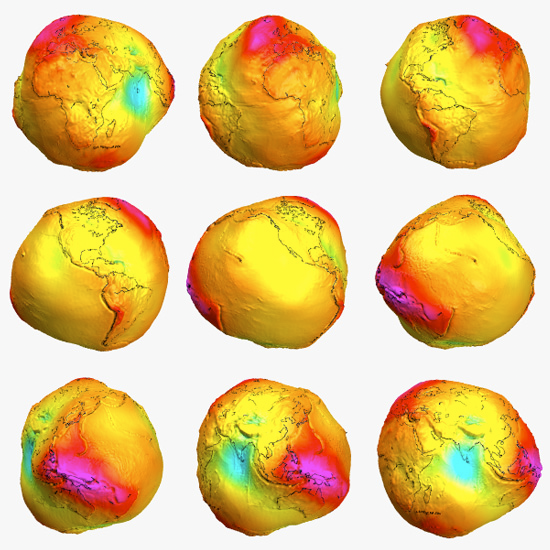
\includegraphics[width=0.9\linewidth]{Resimler/Dünya Modeli/GRACE Potato Model.png}
    \caption{GRACE/GRACE-FO verilerinden türetilen Dünya yerçekimi anomali alanının abartılmış görselleştirmesi.
    Renkler ve yüzey sapmaları, potansiyelin enlem ve boylam boyunca değiştiğini vurgular. Kırmızı renk yüksek gravite alanlarını temsil ederken, mavi renkli bölgeler daha düşük bölgeleri temsil etmektedir.}
    \label{fig:grace_potato}
\end{figure}

\newpage
Bu nedenle gerçek çekim potansiyeli tek başına $r$’nin bir fonksiyonu değildir; enlem ve boylama da bağlıdır.
Başka bir deyişle potansiyel $U(r,\theta,\lambda)$ şeklinde konuma bağlı bir yapı kazanır.
Önceki bölümde elde edilen Legendre ve ilişkili Legendre polinomları bu noktada devreye girer.
Bu fonksiyonlar açısal bağımlılığı düzenli bir biçimde ayrıştırmaya yarar ve küresel harmonikler aracılığıyla potansiyelin enlem ve boylam yönündeki değişimini sistematik olarak ifade etmemizi sağlar.


% ===================== Harmonik Sınıflar =======================
\section{Harmonik Sınıfları}
\label{sec:norm_and_Jn}

Dünya'nın dış bölgesinde ($r>R_E$) kütle yoğunluğu yoktur ($\rho=0$) ve potansiyel
\begin{equation}
\nabla^2 U = 0
\label{eq:laplace_outside}
\end{equation}
Laplace denklemini sağlar.
Önceki bölümde Laplace denkleminin küresel koordinatlarda ayrılmasıyla
boylam yönünde periyodik Fourier modlarının ve enlem yönünde associated Legendre fonksiyonlarının elde edildiği gösterilmişti.
Bu nedenle Dünya için ``doğal'' potansiyel yazımı, küresel harmonik baz üzerinde katsayılandırılmış bir açılımdır; potansiyel
\begin{equation}
U(r,\phi,\lambda)
=
-\frac{\mu}{r}
\left[
1
+
\sum_{\ell=2}^{\infty}
\left(\frac{R_E}{r}\right)^{\ell}
\sum_{m=0}^{\ell}
\overline{P}_{\ell}^{\,m}[\sin\phi]
\left(
\overline{C}_{\ell m}\cos m\lambda
+
\overline{S}_{\ell m}\sin m\lambda
\right)
\right]
\label{eq:earth_potential1}
\end{equation}
\noindent
şeklinde yazılır. Bu denklem, Dünya’nın kütle dağılımındaki düzensizlikleri küresel harmonikler cinsinden ifade eder.

Bu açılımı daha kompakt bir notasyonla ifade etmek için küresel harmonik baz fonksiyonları genellikle $Y_{\ell}^{m}$ ile gösterilir.
Burada $\overline{P}_{\ell}^{\,m}(\sin\phi)$ enlem bağımlılığını, $\cos(m\lambda)$ ve $\sin(m\lambda)$ terimleri ise boylam bağımlılığını taşır.
Gerçek (cos/sin) gösterimde modlar
\[
Y_{\ell, m}^{c}(\phi,\lambda)=\overline{P}_{\ell}^{\,m}[\sin\phi]\cos(m\lambda),
\qquad
Y_{\ell, m}^{s}(\phi,\lambda)=\overline{P}_{\ell}^{\,m}[\sin\phi]\sin(m\lambda)
\]
şeklinde yazılır ve \eqref{eq:earth_potential1} içindeki $\overline{C}_{\ell, m}$ ve $\overline{S}_{\ell, m}$ katsayıları bu modların ağırlıklarını belirler. Jeodezi literatürü ile tutarlılık açısından yaygın olan gerçek katsayılı (cos/sin) gösterim tercih edilmiştir.

\medskip
\noindent
Bu gösterimde $\ell$ (derece) ve $m$ (mertebe) indisleri, küre üzerindeki desenin hem \textbf{ölçeğini} hem de
\textbf{boylama bağlılığını} belirler: $\ell$ büyüdükçe temsil edilen yapılar daha küçük ölçekli hâle gelir;
$m$ ise terimin boylam $\lambda$ boyunca değişimini, yani boylam yönündeki Fourier modunu belirtir.
Bu nedenle küresel harmonikler, $m$’nin aldığı değerlere göre üç temel sınıfta incelenir:
\textbf{zonal} ($m=0$), \textbf{tesseral} ($0<m<\ell$) ve \textbf{sectoral} ($m=\ell$).
İzleyen alt bölümlerde bu sınıflar sırasıyla tanıtılacak; her birinin geometrik yorumu ve
Dünya yerçekimi alanındaki fiziksel karşılıkları incelenecektir.


\begin{center}
\setlength{\fboxsep}{6pt}
\setlength{\fboxrule}{0.6pt}
\fbox{%
\begin{minipage}{0.82\linewidth}
\textbf{Harmonik sınıfları (Zonal--Tesseral--Sectoral)}\\[4pt]
\begin{itemize}
    \item $\boldsymbol{m=0}\ \Rightarrow\ \text{boylamdan bağımsız bantlar (zonal)},$
    \item $\boldsymbol{m=\ell}\ \Rightarrow\ \text{boylam dilimleri (sectoral)},$
    \item $\boldsymbol{0<m<\ell}\ \Rightarrow\ \text{enlem--boylam ızgarası (tesseral)}.$
\end{itemize}
\end{minipage}%
}
\end{center}


% ------------------ Zonal Harmonikler -------------
\newpage
\subsection{Zonal Harmonikler ($m=0$)}
\label{subsec:zonal}

\textbf{Zonal} harmonikler $m=0$ koşuluyla tanımlanır; dolayısıyla \textbf{boylamdan bağımsızdır}
ve yalnızca enlem (veya kolatitüde) değişkenine bağlıdır.
Bu özellik, dönme ekseni etrafındaki eksenel simetriyi temsil eder.
Geometrik olarak zonal bileşenler, küre üzerinde \textbf{enlemlere paralel bantlar}
(kuşaklar) üretir: potansiyel (ve dolayısıyla yerçekimi) boylama göre değişmez, yalnızca enlemle değişir.

Zonal terimler çoğu zaman en baskın şekil sapmalarını taşır. Özellikle $\ell=2$ zonal terimi
(çoğu kaynakta $J_2$ ile ilişkilendirilir), Dünya’nın kutuplardan basık ve ekvatordan şişkin olmasını
(\emph{oblateness}) birinci mertebeden temsil eder. Daha yüksek dereceli zonal terimler ($\ell=3,4,\dots$),
bu genel şeklin üzerine daha ince ölçekli düzeltmeler ekleyerek bant yapısını giderek daha sık hâle getirir.

\begin{figure}[h]
    \centering
    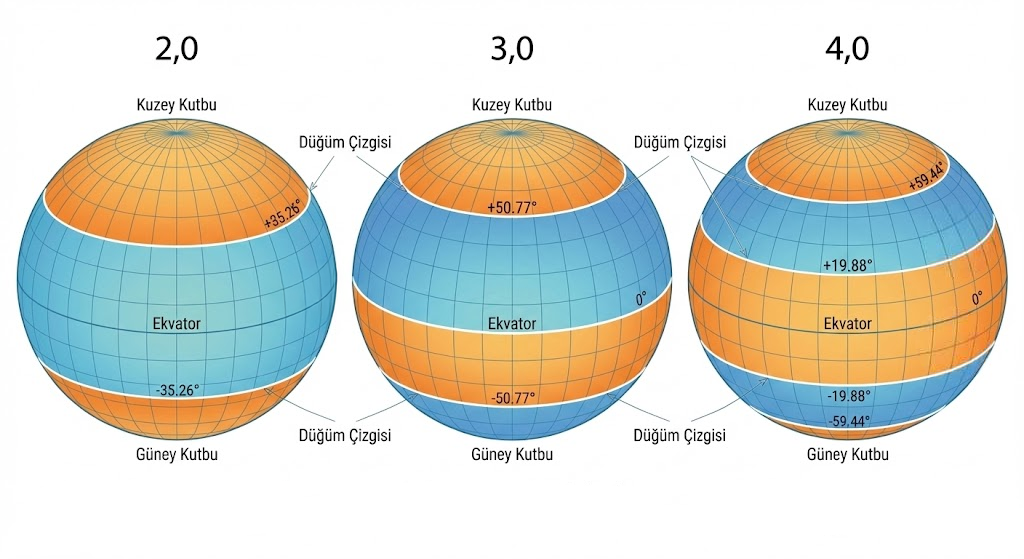
\includegraphics[width=1\linewidth]{Resimler/Dünya Modeli/Zonal Harmonikler.png}
    \caption{Zonal harmonikler ($m=0$) için $\ell=2,3,4$ örnekleri. Renkli bantlar (mavi pozitif, turuncu negatif) bölgeleri, bant sınırları ise düğüm dairelerini (nodal çizgileri) göstermektedir.}
    \label{fig:zonal_harmonics}
\end{figure}

\medskip
Şekil~\ref{fig:zonal_harmonics}’te görüldüğü üzere, zonal harmonikler için $m=0$ olduğundan
boylam bağımlılığı ortadan kalkar. Bu nedenle düğüm çizgileri \textbf{enlemlere paralel kapalı daireler} oluşturur.
Zonal bir harmonikte \textbf{$\ell$ adet düğüm dairesi} ve buna karşılık
\textbf{$\ell+1$ adet bant bölgesi} meydana gelir.


\subsubsection*{Düğüm enlemlerinin bulunması}

Zonal harmoniklerde ($m=0$) düğüm daireleri, açısal kısmın (enlem bağımlılığının) sıfır olduğu
enlemlere karşılık gelir. Bu nedenle düğüm enlemleri $\phi_i$, aşağıdaki koşuldan elde edilir:
\begin{equation}
P_\ell\!\bigl[\sin\phi_i\bigr]=0,
\qquad 
\phi_i\in\left(-\frac{\pi}{2},\frac{\pi}{2}\right).
\label{eq:zonal_nodes_phi}
\end{equation}
Burada $\phi$ jeosentrik enlemdir. Kökler $\phi=0$ (ekvator) etrafında simetriktir; bunun nedeni
Legendre polinomlarının parite özelliği $P_\ell[-x]=[-1]^\ell P_\ell(x)$’tir. Dolayısıyla bant yapısı
ekvatora göre düzenli bir simetri sergiler: $\ell$ tek ise ekvator bir düğümdür, $\ell$ çift ise
ekvator düğüm oluşturmaz.

\bigskip
\noindent
Düğüm enlemlerini bulmak için \eqref{eq:zonal_nodes_phi}’de $x=\sin\phi$ dönüşümü yapılır ve
$P_\ell(x)=0$ denkleminin kökleri hesaplanır. Küçük dereceler için bu kökler kapalı formda
açıkça gösterilebilir:

\begin{itemize}
\item \textbf{$\ell=2$:}
\[
P_2(x)=\tfrac{1}{2}(3x^2-1)
\quad\Rightarrow\quad
P_2(x)=0 \;\Rightarrow\; x=\pm \tfrac{1}{\sqrt{3}}.
\]
\[
\phi=\arcsin(x)=\pm \arcsin\!\left(\tfrac{1}{\sqrt{3}}\right)=\pm 35.26^\circ.
\]

\item \textbf{$\ell=3$:}
\[
P_3(x)=\tfrac{1}{2}(5x^3-3x)=\tfrac{1}{2}x(5x^2-3)
\quad\Rightarrow\quad
P_3(x)=0 \;\Rightarrow\; x=0,\ \pm\sqrt{\tfrac{3}{5}}.
\]
\[
\phi=\arcsin(x)=0^\circ,\qquad
\phi=\pm \arcsin\!\left(\sqrt{\tfrac{3}{5}}\right)=\pm 50.77^\circ.
\]

\item \textbf{$\ell=4$:}
\[
P_4(x)=\tfrac{1}{8}(35x^4-30x^2+3)
\quad\Rightarrow\quad
P_4(x)=0 \;\Rightarrow\; x=\pm 0.339981,\ \pm 0.861136.
\]
\[
\phi=\arcsin(x)
\quad\Rightarrow\quad
\phi\approx \pm 19.88^\circ,\ \pm 59.44^\circ.
\]

\end{itemize}

\begin{table}[h]
\centering
\caption{Zonal harmonikler için elde edilen düğüm enlemleri ($\phi_i$).}
\label{tab:zonal_nodes}
\renewcommand{\arraystretch}{1.25}
\begin{tabular}{@{} c c l @{}} 
\toprule
\textbf{Derece ($\ell$)} & \textbf{Düğüm Sayısı} & \textbf{Düğüm Enlemleri [deg]} \\
\midrule
2 & 2 & $\pm 35.26^\circ$ \\
3 & 3 & $0^\circ,\ \pm 50.77^\circ$ \\
4 & 4 & $\pm 19.88^\circ,\ \pm 59.44^\circ$ \\
\bottomrule
\end{tabular}
\end{table}



% --------------- Sectoral Harmonikler ----------------
\subsection{Sectoral Harmonikler ($m=\ell$)}
\label{subsec:sectoral}

\textbf{Sectoral} terimler $m=\ell$ koşuluyla tanımlanır.
Bu sınıfta hem enleme hem de boylama bağlılık en güçlü halini alır. Sectoral harmonikler küreyi boylam doğrultusunda ``dilimlere'' ayıran bir desen üretir: boylamda değişim maksimumdur ve desen, meridyenler boyunca sıkça tekrar eder.
$m$ (dolayısıyla $\ell$) arttıkça dilim sayısı artar; yani daha fazla sayıda, daha dar boylam bölgesi oluşur. Bu ``dilimlenme'' karakteri, farklı $\ell$ değerleri için örnek olarak
Şekil~\ref{fig:sectoral_harmonics}'te görülebilir.

\medskip
Fiziksel açıdan sectoral bileşenler,
tam eksen-simetrik olmayan ve belirli boylamlarda tekrarlayan kütle düzensizliklerini
temsil etmede etkilidir. Bu tür terimler, özellikle
tesseral/sectoral bileşenlerin baskın olduğu gezegenlerde veya bölgesel kütle anomalilerinde
yerçekimi alanına belirgin katkılar yapabilir.

\begin{figure}[h]
    \centering
    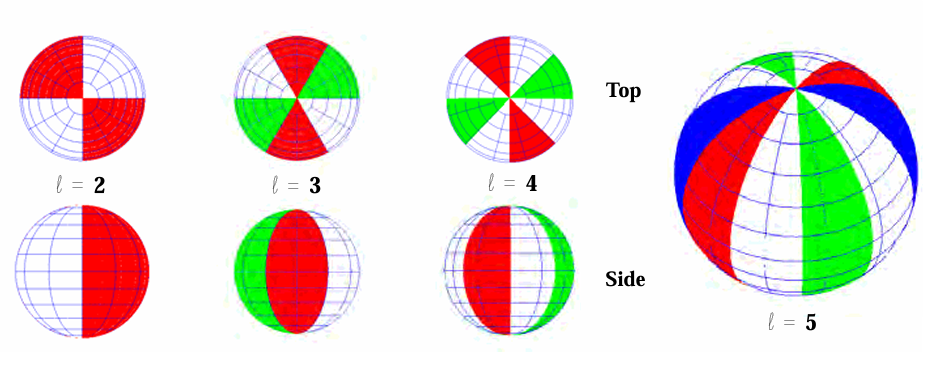
\includegraphics[width=1\linewidth]{Resimler/Dünya Modeli/Sectoral Harmonikler.png}
    \caption{Sectoral harmonikler ($m=\ell$) için örnek desenler: $\ell=2,3,4$ durumlarında üst (Top) ve yan (Side) görünüşler. Renkli bölgeler negatif, beyaz bölgeler ise pozitif katkıları göstermekte.}
    \label{fig:sectoral_harmonics}
\end{figure}


% ------------- Tesseral Harmonikler --------------

\subsection{Tesseral Harmonikler ($0<m<\ell$)}
\label{subsec:tesseral}

\textbf{Tesseral} terimler $0<m<\ell$ aralığıyla tanımlanır.
Bu sınıf, zonal ($m=0$) ile sectoral ($m=\ell$) arasında bir ``ara bölge'' gibidir: hem enleme hem de boylama bağlıdır, ancak sectoral kadar ``tam dilimli'' bir yapı vermez. Ortaya çıkan desen genellikle küre üzerinde bir \textbf{ızgara/karo} \emph{tessera}) görünümüne benzetilir; çünkü hem meridyen hem paralel yönünde işaret değişimleri (sıfır çizgileri) görülür.
Bu karo-benzeri desen karakteri, farklı $(\ell,m)$ çiftleri için örnek olarak Şekil~\ref{fig:tesseral_harmonics}'te gösterilmiştir.

\begin{figure}[h]
    \centering
    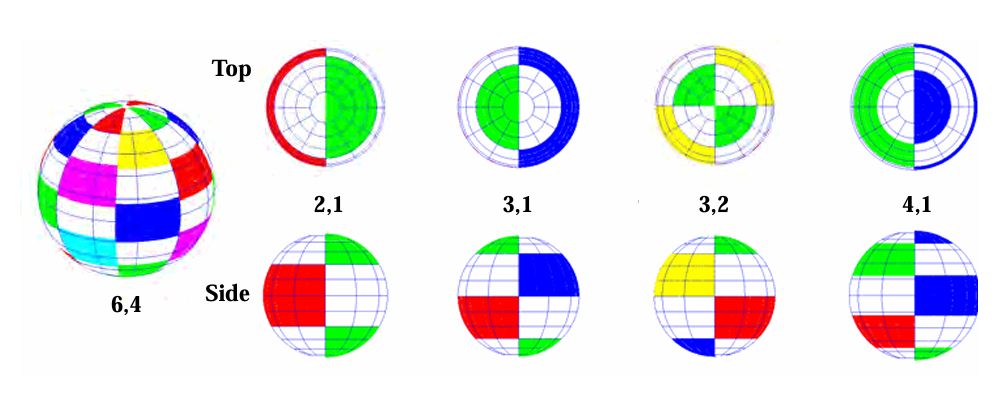
\includegraphics[width=1\linewidth]{Resimler/Dünya Modeli/Tesseral Harmonikler.png}
    \caption{Tesseral harmonikler ($0<m<\ell$) için örnek desenler: seçili $(\ell,m)$ çiftlerinde üst (Top) ve yan (Side) görünüşlerde oluşan ``karo'' (\emph{tessera}) benzeri işaret değişimleri. Renkli bölgeler negatif, beyaz bölgeler ise pozitif katkıları göstermekte.}
    \label{fig:tesseral_harmonics}
\end{figure}

Bazı kaynaklarda sectoral terimler, tesseral sınıfının
özel bir alt durumu gibi sunulabilir (çünkü $m=\ell$ de temelde boylama bağımlıdır). Ancak uygulamada, $m=\ell$ durumunun desen karakteri ve matematiksel davranışı (Şekil~\ref{fig:sectoral_harmonics}'teki belirgin ``dilimlenme'' gibi) daha ayırt edici olduğu için sectoral terimler çoğu zaman ayrı bir başlık altında incelenir.


% ================ J_l Terimlerinin Etkisi =============
\newpage
\section{\texorpdfstring{$J_\ell$}{J\_l} Terimleri ve Etkileri}

Zonal harmonikler ($m=0$) söz konusu olduğunda, literatürde iki farklı katsayı gösterimine sıklıkla rastlanır. Kullanım yaygınlığı nedeniyle $C_{\ell,0}$ katsayısı yerine genellikle $J_{\ell}$ notasyonu tercih edilmektedir. Ancak bu iki notasyon arasında bir işaret farkı bulunduğu unutulmamalıdır:

\begin{equation}
    C_{\ell,0} = - J_{\ell}
    \label{eq:C_J_relation}
\end{equation}

% ----------------- J_l ve C_bar arasındaki ilişki ---------
\subsection{\texorpdfstring{$J_\ell$ ile $\bar C_{\ell,0}$ İlişkisi}{J\_l ile C\_bar\_\{l,0\} İlişkisi}}
\label{subsec:Jn_relation}

Literatürde yerçekimi potansiyeli, klasik olarak \textbf{normalize edilmemiş} $J_{\ell}$ katsayıları kullanılarak şu formda ifade edilir:
\begin{equation}
U(r,\phi)
=
-\frac{\mu}{r}
\left[
1
+
\sum_{\ell=2}^{\infty}
J_\ell
\left(\frac{R_E}{r}\right)^\ell
P_\ell[\sin\phi]
\right].
\label{eq:zonal_potential}
\end{equation}
Burada $P_\ell[\sin\phi]$ yalnızca enleme bağlı Legendre polinomudur; dolayısıyla $m = 0$ olduğundan bileşenlerinde boylam etkisi yoktur. $J_\ell$ katsayısı, $\ell$ dereceli zonal harmonik katkının büyüklüğünü belirler. Özellikle $\ell=2$ için $J_2$, Dünya’nın basıklığını (\emph{oblateness}) temsil eden en baskın terimdir.

Ancak modern jeodezik modeller (örneğin EGM96, EGM2008), katsayı verilerini küresel harmonik bazının ortogonalliğini korumak amacıyla \textbf{tam-normalize} (\emph{fully normalized}) $\bar C_{\ell,0}$ formunda sunar. Bu iki gösterim fiziksel olarak eşdeğerdir; aralarındaki fark, normalizasyon tanımından kaynaklanan sabit bir ölçek çarpanıdır.

Jeodezide yaygın kullanılan dönüşüm şöyledir:
\begin{equation}
J_\ell = -\sqrt{2\ell+1}\,\bar C_{\ell,0},
\qquad \bar S_{\ell,0}=0
\label{eq:Jn_Cn0_relation}
\end{equation}
Bu ifadede $\sqrt{2\ell+1}$ çarpanı \textbf{normalizasyon farkını} temsil eder. $m=0$ (zonal) terimler için sinüs katsayısı bulunmadığından $\bar S_{\ell,0}=0$ olarak belirtilir.

Örneğin en sık kullanılan $\ell=2$ terimi için bu ilişki
\begin{equation}
J_2 = -\sqrt{5}\,\bar C_{2,0}
\label{eq:J2_C20}
\end{equation}
haline gelir. Dolayısıyla bir yerçekimi modelinden veri alınırken, katsayıların \textbf{normalize mi yoksa normalize edilmemiş mi} olduğuna ve kullanılan işaret konvansiyonuna mutlaka dikkat edilmelidir. Aksi halde, aynı fiziksel büyüklük farklı sayısal değerlerle ifade edileceğinden analizlerde ölçek hataları oluşabilir.

% ------------------ Oblateness ------------------
\newpage
\subsection{$J_2$: Basıklık (Oblateness)}
\label{subsec:J2_physical}

Zonal terimler içinde pratikte en baskın olanı $J_2$’dir.
Bunun temel nedeni, Dünya’nın küreden sapmasının en büyük bileşeninin
ekvator şişkinliği (kutuplardan basıklık) olmasıdır.
Basıklık (\emph{oblateness}) şu şekilde tanımlanır:
\begin{equation}
    oblateness = \frac{R_{ekvator} - R_{kutup}}{R_{ekvator}}
    \label{eq:oblateness}
\end{equation}
Dünya için yaklaşık $R_{ekvator} \approx 6378\,\mathrm{km}$ ve $R_{kutup} \approx 6357\,\mathrm{km}$ alındığında
\[
oblateness \approx \frac{6378-6357}{6378} \approx 3.29\times 10^{-3}
\]
bulunur (daha hassas yarıçap değerleriyle bu oran $\sim 3.35\times 10^{-3}$ mertebesindedir).

Burada önemli nokta şudur: \eqref{eq:oblateness} \textbf{geometrik} bir ölçüdür; $J_2$ ise Dünya’nın kütle dağılımının
\textbf{ikinci derece zonal} bileşenini (gravitasyonel ``quadrupole'') temsil eder.
İkisi birebir aynı nicelik değildir; ancak Dünya’daki ekvator şişkinliği hem şekli hem de kütle dağılımını belirgin biçimde
küresel simetriden saptırdığı için, pratikte en baskın zonal katsayının $J_2$ olması beklenir.

\eqref{eq:zonal_potential} içinde yalnızca $\ell=2$ terimini tutup
$P_2[x]=\tfrac12(3x^2-1)$ ve $x=\sin\phi$ yazarsak,
$J_2$’nin potansiyele katkısı enleme bağlı, ``bant'' yapılı bir düzeltme olarak görülür:
ekvator civarında ve kutuplara yakın bölgelerde potansiyel/ivme dağılımı farklılaşır.
Bu tür bir fark, her turda tekrar tekrar etki ettiği için yörünge elemanlarında \textbf{birikimli} (seküler) değişimlere yol açabilir.
Bu nedenle $J_2$, iki-cisim yaklaşımına eklenen \textbf{ilk düzeltme} katsayısı olarak çoğu yörünge probleminde ayrıcalıklı bir yere sahiptir.

Tipik büyüklük olarak
\[
J_2 \approx 1.08263\times10^{-3}
\]
mertebesindedir (seçilen yerçekimi modeli ve işaret/normalizasyon konvansiyonuna bağlı küçük farklar olabilir).
Bu değer, $J_2$’nin neden çoğu uygulamada ``ilk düzeltme'' olarak ele alındığını açıklar:
$J_2$ ihmal edildiğinde, özellikle LEO’da $\Omega$ ve $\omega$ sürüklenmeleri kısa sürede büyük hatalara dönüşür.


% ============================================================
% 2.1 -- 2.3 : J2 etkisi için ortak kurulum + GVE/LPE ile türetim
% ============================================================

\subsection*{RTN Ayrışımı}
\label{subsec:J2_setup}

Dünya’nın (yaklaşık) eksenel simetrik basıklığını temsil eden $J_2$ teriminin yörünge elemanlarına etkisini iki farklı formalizmle elde edebiliriz:
(i) Gauss Değişim Denklemleri (GVE) ve
(ii) Lagrange Gezegen Denklemleri (LPE).
Her iki yaklaşım da aynı fiziksel sonucu verir; fark, birinin doğrudan \textbf{ivme} (kuvvet) bileşenleri üzerinden, diğerinin ise \textbf{bozucu potansiyel} üzerinden ilerlemesidir.

\paragraph{Kepler elemanları ve yardımcı büyüklükler.}
Klasik yörünge (\emph{osculating}) elemanları
\[
(a,\;e,\;i,\;\Omega,\;\omega,\;M)
\]
kullanıyoruz. Gerçek anomali (\emph{True Anomaly}) $f$ için , enlem argümanı (\emph{argument of latitude}):
\[
u \;\triangleq\; \omega + f
\]
olarak tanımlıdır. Yarı parametre (\emph{semi-latus rectum})
\[
p \;\triangleq\; a(1-e^2),\qquad
r \;=\; \frac{p}{1+e\cos f}.
\]
Özgül açısal momentum büyüklüğü
\[
h \;\triangleq\; \|\mathbf r\times \mathbf v\| \;=\; \sqrt{\mu p},
\]
ve ortalama hareket
\[
n \;\triangleq\; \sqrt{\frac{\mu}{a^3}}
\]
şeklindedir. Burada $\mu=GM$ Dünya’nın çekim parametresidir.

\paragraph{RTN (Radial--Transverse--Normal) çerçevesi.}
Konum vektörü $\mathbf r$ ve hız vektörü $\mathbf v$ ile
\[
\hat{\mathbf R} \triangleq \frac{\mathbf r}{r},\qquad
\hat{\mathbf N} \triangleq \frac{\mathbf h}{h},\qquad
\hat{\mathbf T} \triangleq \hat{\mathbf N}\times \hat{\mathbf R}
\]
birim vektörleri tanımlanır.
Herhangi bir bozucu ivme $\mathbf a_p$ RTN bileşenlerine ayrıştırılır:
\[
a_R \triangleq \mathbf a_p\cdot \hat{\mathbf R},\qquad
a_T \triangleq \mathbf a_p\cdot \hat{\mathbf T},\qquad
a_N \triangleq \mathbf a_p\cdot \hat{\mathbf N},
\]
dolayısıyla
\[
\mathbf a_p \;=\; a_R\hat{\mathbf R} + a_T\hat{\mathbf T} + a_N\hat{\mathbf N}.
\]

\paragraph{$J_2$ potansiyeli ve bozucu fonksiyon.}
Dünya’nın eksenel simetrik (zonal) $J_2$ düzeltmesi ile,
yerçekimi potansiyelini (birim kütle başına) şu şekilde yazıyoruz:

\begin{equation}
U(r,\phi) \;=\; -\frac{\mu}{r}\Bigg[1 - J_2\Big(\frac{R_E}{r}\Big)^2 P_2[\sin\phi]\Bigg],
\qquad
P_2[x]=\frac{1}{2}(3x^2-1),
\label{eq:U_J2_def}
\end{equation}

burada $R_E$ ekvator yarıçapı ve $\phi$ jeosantrik enlemdir.
Merkezi ($-\mu/r$) terimi ayırırsak, $J_2$’ye karşılık gelen \textbf{bozucu potansiyel}
\[
\mathcal R_{J_2} \;\triangleq\; U + \frac{\mu}{r}
\;=\; \frac{\mu R_E^2 J_2}{2r^3}\,(3\sin^2\phi - 1)
\]
olur. Eksenel simetri nedeniyle $\phi$’yi yörünge elemanlarıyla bağlamak için
\[
z = r\sin\phi,\qquad
z = r\sin i \sin u
\;\;\;\Rightarrow\;\;\;
\sin\phi = \sin i \sin u
\]
kullanacağız.

\paragraph{$J_2$ ivmesinin RTN bileşenleri.}
$J_2$ etkisini GVE’de kullanmak için $\mathbf a_{J_2} = -\nabla \mathcal R_{J_2}$
ivmesini RTN’ye projekte ederiz. Standart sonuçlar şu biçimdedir:
\begin{subequations}\label{eq:J2_RTN_acc}
\begin{align}
a_R \;&=\; -\frac{3}{2}\,J_2\,\frac{\mu R_E^2}{r^4}\Big(1 - 3\sin^2 i\,\sin^2 u\Big), \label{eq:aR_J2}\\
a_T \;&=\; -3\,J_2\,\frac{\mu R_E^2}{r^4}\,\sin^2 i\,\sin u\,\cos u, \label{eq:aT_J2}\\
a_N \;&=\; -3\,J_2\,\frac{\mu R_E^2}{r^4}\,\sin i\,\cos i\,\sin u. \label{eq:aN_J2}
\end{align}
\end{subequations}
Bu üç bileşen, GVE veya Cowell propagasyonunda doğrudan kullanılabilir.

\paragraph{Yörünge ortalaması (seküler terimler).}
Özel yörüngeler (Sun-synchronous, kritik eğim/Molniya vb.) çoğunlukla seküler (uzun dönemli) oranlara dayanır. Bu yüzden, bir periyot boyunca \textbf{yörünge ortalaması} operatörünü tanımlıyoruz:
\begin{equation}
\big\langle (\cdot)\big\rangle \;\triangleq\;
\frac{1}{2\pi}\int_0^{2\pi} (\cdot)\, dM
\;=\;\frac{1}{2\pi}\int_0^{2\pi} (\cdot)\,\frac{r^2}{a^2\sqrt{1-e^2}}\,df.
\label{eq:orbit_average}
\end{equation}
Bu ortalamada kısa-periyotlu (periyot içinde salınan) terimler sıfıra gider, seküler drift oranları kalır.

% ------------------------------------------------------------
\subsection{Gauss Değişim Denklemleri (GVE)}
\label{subsec:J2_GVE}

GVE, bozucu ivmenin RTN bileşenleri cinsinden yörünge eleman türevlerini verir. Özellikle $\dot\Omega$ ve
$\dot\omega$ seküler oranları kritik olduğu için, önce ilgili GVE formüllerini yazıyoruz (klasik elemanlar için):

{%
\setlength{\fboxsep}{6pt}% kutu iç boşluğu
\setlength{\fboxrule}{0.6pt}% kutu çizgi kalınlığı
\begin{center}
\fbox{%
\begin{minipage}{0.97\linewidth}
\begin{subequations}\label{eq:GVE_basic}
\begin{align}
\dot a \;&=\; \frac{2a^2}{h}\Big[e\sin f\,a_R + \frac{p}{r}a_T\Big], \label{eq:GVE_a}\\[3pt]
\dot e \;&=\; \frac{1}{h}\Big[p\sin f\,a_R + \big((p+r)\cos f + re\big)a_T\Big], \label{eq:GVE_e}\\[3pt]
\dot i \;&=\; \frac{r\cos u}{h}\,a_N, \label{eq:GVE_i}\\[3pt]
\dot\Omega \;&=\; \frac{r\sin u}{h\sin i}\,a_N, \label{eq:GVE_Om}\\[3pt]
\dot\omega \;&=\; \frac{1}{he}\Big[-p\cos f\,a_R + (p+r)\sin f\,a_T\Big]
\;-\;\frac{r\sin u}{h}\cot i\,a_N, \label{eq:GVE_om}\\[3pt]
\dot f \;&=\; \frac{h}{r^2} + \frac{1}{he}\Big(p\cos f\,a_R - (p+r)\sin f\,a_T\Big). \label{eq:gauss_f}
\end{align}
\end{subequations}
\end{minipage}%
}%
\end{center}
}%

Burada $u=\omega+f$ ve $p=a(1-e^2)$’dir.



\subsubsection*{(i) Düğüm hattı dönümü: $\langle\dot\Omega\rangle$}

\eqref{eq:GVE_Om} içine $a_N$ bileşenini \eqref{eq:aN_J2} yerleştiriyoruz:
\[
\dot\Omega
\;=\;\frac{r\sin u}{h\sin i}\Bigg(-3J_2\frac{\mu R_E^2}{r^4}\sin i\cos i\,\sin u\Bigg)
\;=\; -\frac{3J_2\mu R_E^2}{h}\,\frac{\cos i}{r^3}\,\sin^2 u.
\]
Yörünge ortalaması alındığında,
$\sin^2 u = \tfrac12(1-\cos 2u)$ olduğundan $\cos 2u$ içeren terimler periyot boyunca
sıfıra gider ve
\[
\Big\langle \frac{\sin^2 u}{r^3}\Big\rangle
\;=\;\frac{1}{2}\Big\langle \frac{1}{r^3}\Big\rangle.
\]
Ayrıca bilinen sonuç
\[
\Big\langle \frac{1}{r^3}\Big\rangle
\;=\;\frac{1}{a^3(1-e^2)^{3/2}}
\]
kullanılır. Böylece
\begin{equation}
\boxed{
\big\langle \dot\Omega \big\rangle
\;=\; -\frac{3}{2}\,J_2\,n\Big(\frac{R_E}{p}\Big)^2\cos i
}
\label{eq:Omega_secular_J2}
\end{equation}
elde edilir.

\noindent
Bu bağıntı iki kritik yorumu doğrudan verir:
(i) seküler RAAN driftinin büyüklüğü $\cos i$ ile ölçeklenir; dolayısıyla eğim değiştikçe drift hızı değişir, (ii) $i=90^\circ$ (polar yörünge) için $\cos i=0$ olduğundan seküler RAAN drift sıfırlanır. Buna karşın, osculating (kısa-periyot) salınımlar tek tek yörüngeler üzerinde gözlenmeye devam eder.

\begin{figure}[h]
    \centering
    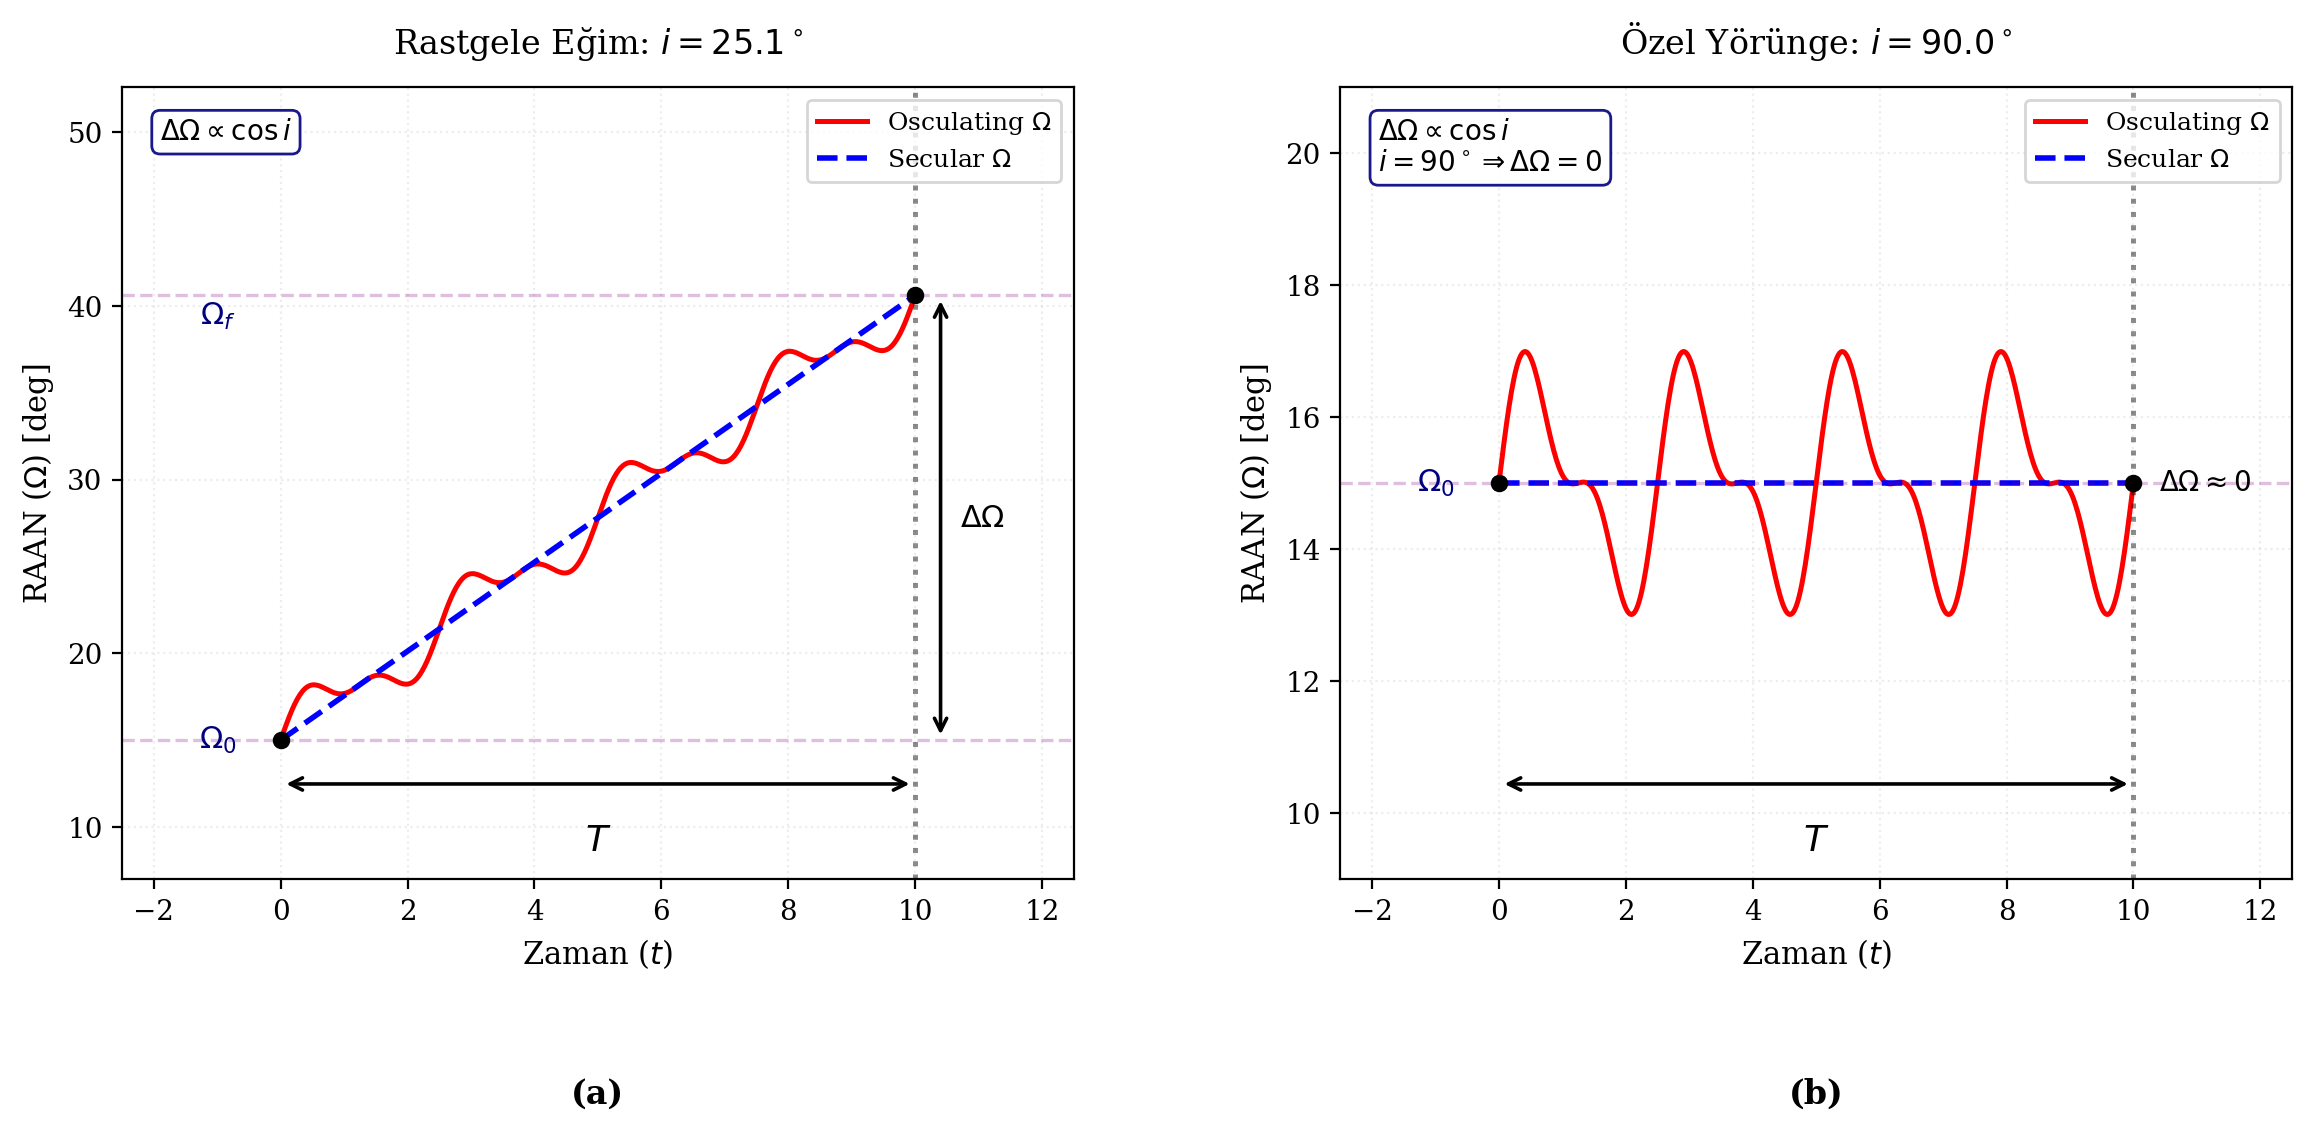
\includegraphics[width=1\linewidth]{Resimler/Dünya Modeli/RAAN Shift.png}
    \caption{J$_2$ etkisi altında RAAN ($\Omega$) değişimi: osculating (kırmızı) ve seküler/ortalama (mavi kesikli) bileşenlerin karşılaştırılması.
    (a) Genel bir eğiklikte $\Delta\Omega \neq 0$ olup seküler drift lineerdir.
    (b) Polar yörüngede ($i=90^\circ$) $\cos i = 0$ nedeniyle seküler drift yaklaşık sıfırdır; yalnızca kısa-periyot salınımlar kalır.}
    \label{fig:raan_shift_j2}
\end{figure}



\subsubsection*{(ii) Perigee dönümü: $\langle\dot\omega\rangle$}

\eqref{eq:GVE_om} ifadesine $a_R,a_T,a_N$ (bkz. \eqref{eq:J2_RTN_acc}) yerleştirilir.
Bu adımda $\sin u\cos u$ ve $\sin^2u$ gibi terimler oluşur. Periyot ortalamasında
$\sin 2u$ içeren terimler sıfıra gider; $\sin^2u$ ve $\cos^2u$ terimleri ise
$\tfrac12\langle 1/r^3\rangle$ şeklinde katkı verir.
Ayrıca $h=\sqrt{\mu p}$ ve $\langle 1/r^3\rangle$ kullanılarak sadeleştirilince,
seküler perigee dönüm oranı
\begin{equation}
\boxed{
\big\langle \dot\omega \big\rangle
\;=\; \frac{3}{4}\,J_2\,n\Big(\frac{R_E}{p}\Big)^2\big(5\cos^2 i - 1\big)
}
\label{eq:omega_secular_J2}
\end{equation}
olarak bulunur.

\begin{figure}[h]
    \centering
    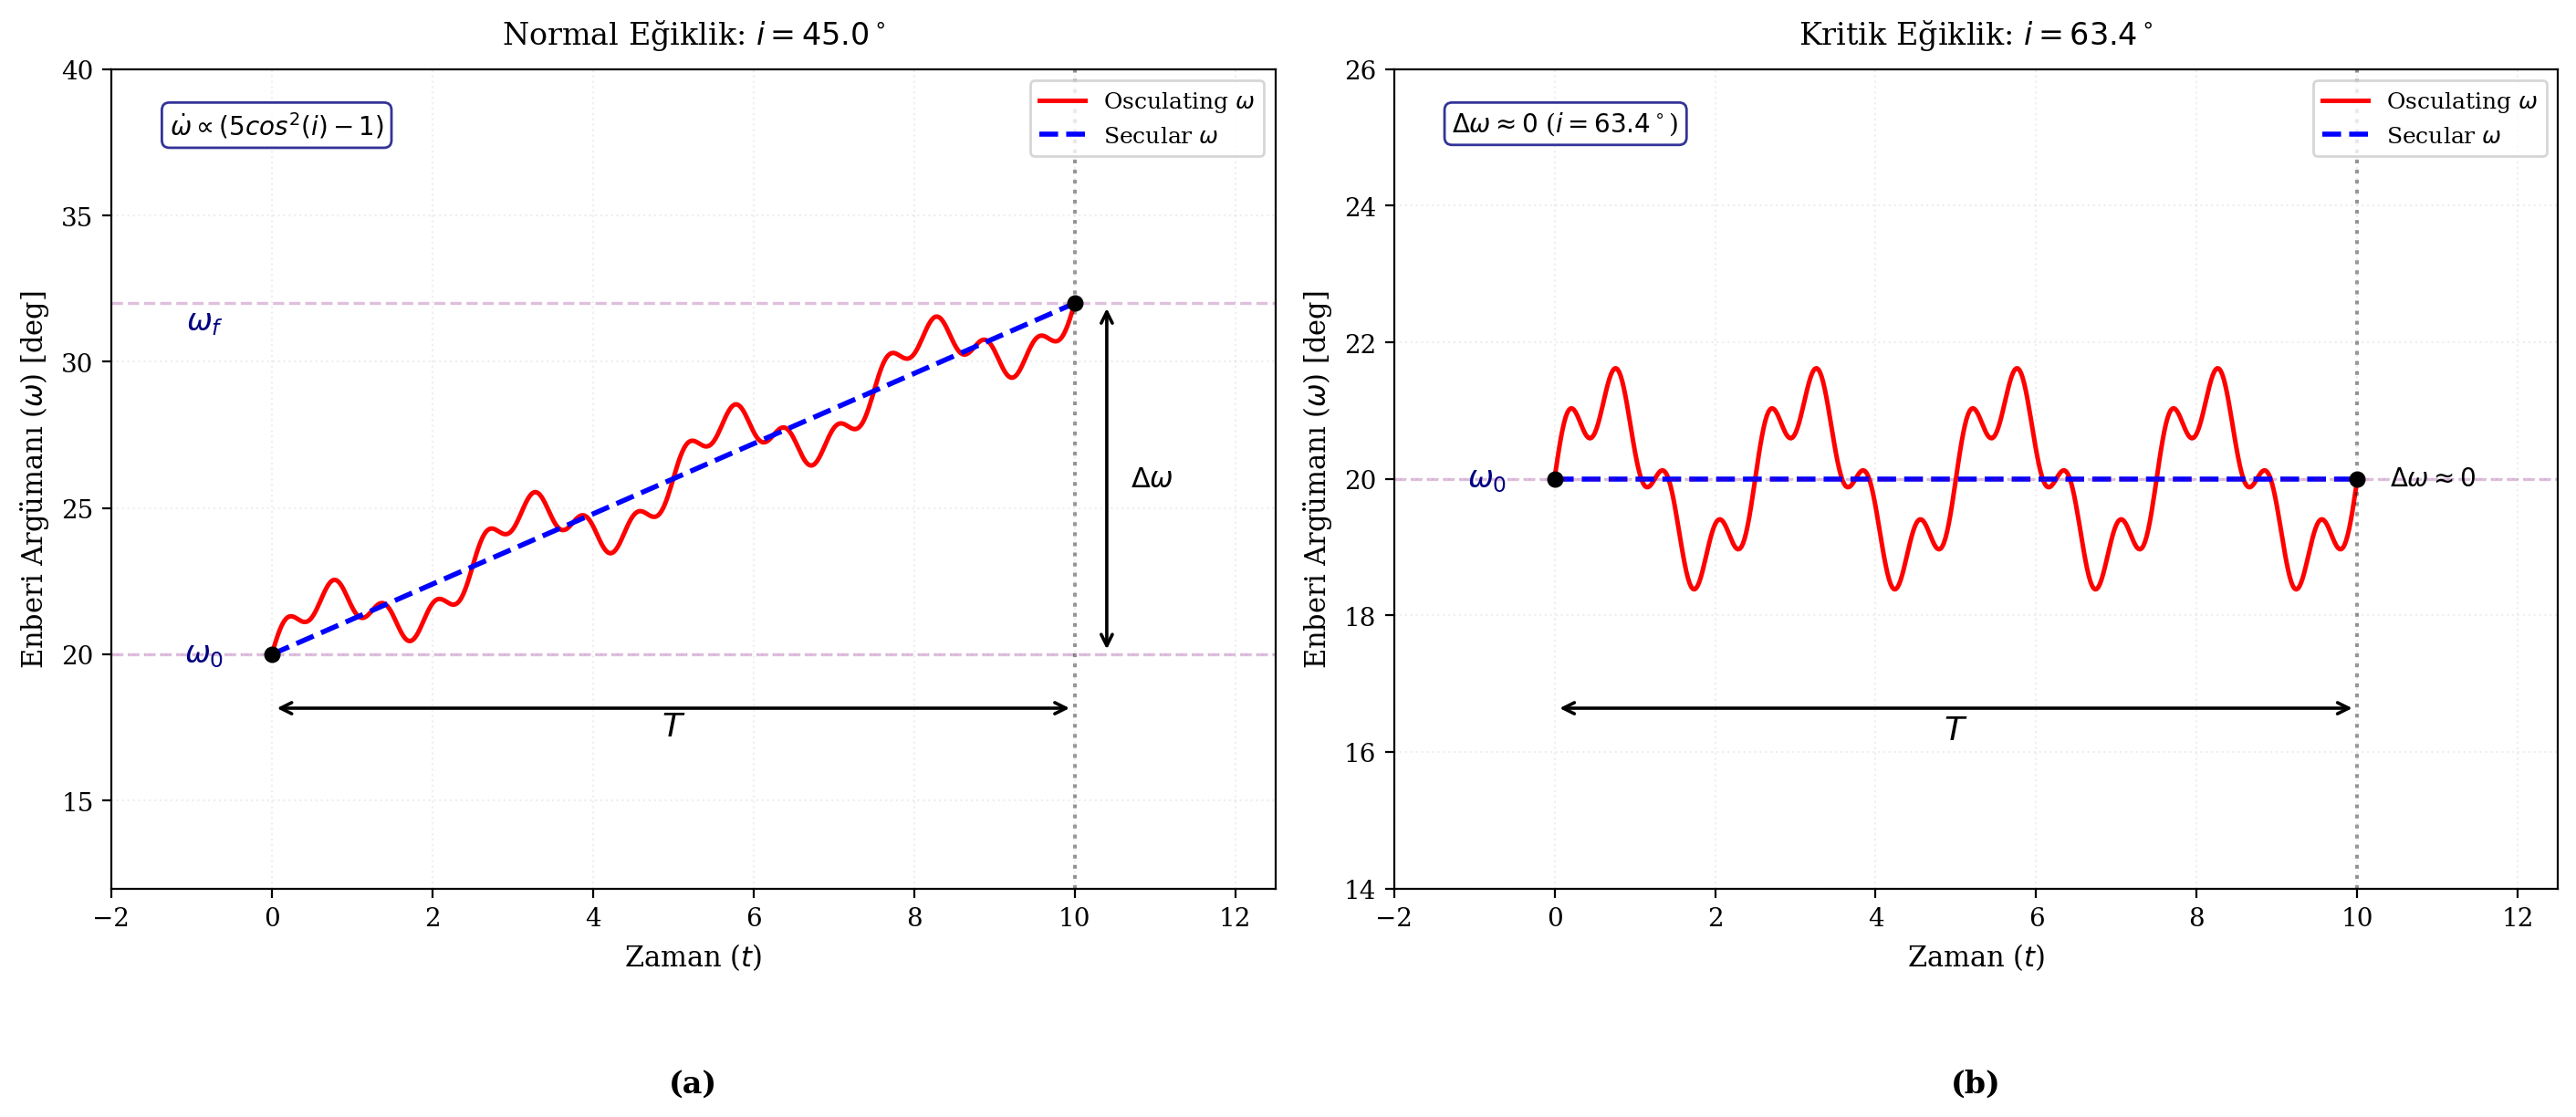
\includegraphics[width=0.95\linewidth]{Resimler/Dünya Modeli/Enberi Shift.png}
    \caption{J$_2$ etkisi altında enberi argümanı ($\omega$) değişimi: osculating (kırmızı) ve seküler/ortalama (mavi kesikli) bileşenlerin karşılaştırılması.
    (a) Genel bir eğiklikte $\Delta\omega \neq 0$ olup seküler drift lineerdir.
    (b) Kritik eğiklikte ($i\approx 63.4^\circ$) $5\cos^2 i - 1 \approx 0$ olduğundan seküler perigee drift yaklaşık sıfırdır; kısa-periyot salınımlar baskın kalır.}
    \label{fig:perigee_shift_j2}
\end{figure}

\noindent
\eqref{eq:omega_secular_J2}’nin en önemli sonucu, \textbf{kritik eğiklik} koşuludur:
\[
\big\langle \dot\omega \big\rangle \approx 0
\;\Rightarrow\;
5\cos^2 i -1 \approx 0
\;\Rightarrow\;
i \approx \arccos\sqrt{\frac{1}{5}} \approx 63.435^\circ.
\]
Bu durumda perigee argümanı uzun dönemde lineer drift göstermemeye yaklaşır; fakat osculating $\omega$
üzerindeki kısa-periyot salınımlar yine devam eder. Şekil \ref{fig:perigee_shift_j2}’de iki farklı eğiklik değeri için seküler ve gerçek bileşenlerin karşılaştırılması verilmiştir.




\medskip
Bu sonuçlar $J_2$ etkisinin tasarım açısından neden güçlü olduğunu açıkça gösterir:

\begin{itemize}
\item \textbf{İrtifa bağımlılığı:} Etki yaklaşık olarak $\left(R/p\right)^2$ ile ölçeklenir.
LEO’da ($p$ küçük) precesyonlar büyüktür; irtifa arttıkça hızla zayıflar.

\item \textbf{Eğim bağımlılığı:} $\dot{\Omega}$ doğrudan $\cos i$ ile, $\dot{\omega}$ ise $(5\cos^2 i-1)$ ile kontrol edilir. Dolayısıyla aynı irtifada dahi $ i $ seçimi ile istenen precesyon hızı ayarlanabilir.

\item \textbf{İşaret (yön) bilgisi:} $\dot{\Omega}$’nın negatif işareti, prograd yörüngelerde ($0^\circ<i<90^\circ$) düğüm gerilemesinin tipik olduğunu; retrograd yörüngelerde
($90^\circ<i<180^\circ$) ise işaretin tersine döndüğünü gösterir. Bu özellik, özellikle Güneş-eşzamanlı (SSO) yörünge tasarımında kritik rol oynar.

\end{itemize}

\begin{figure}[h]
    \centering
    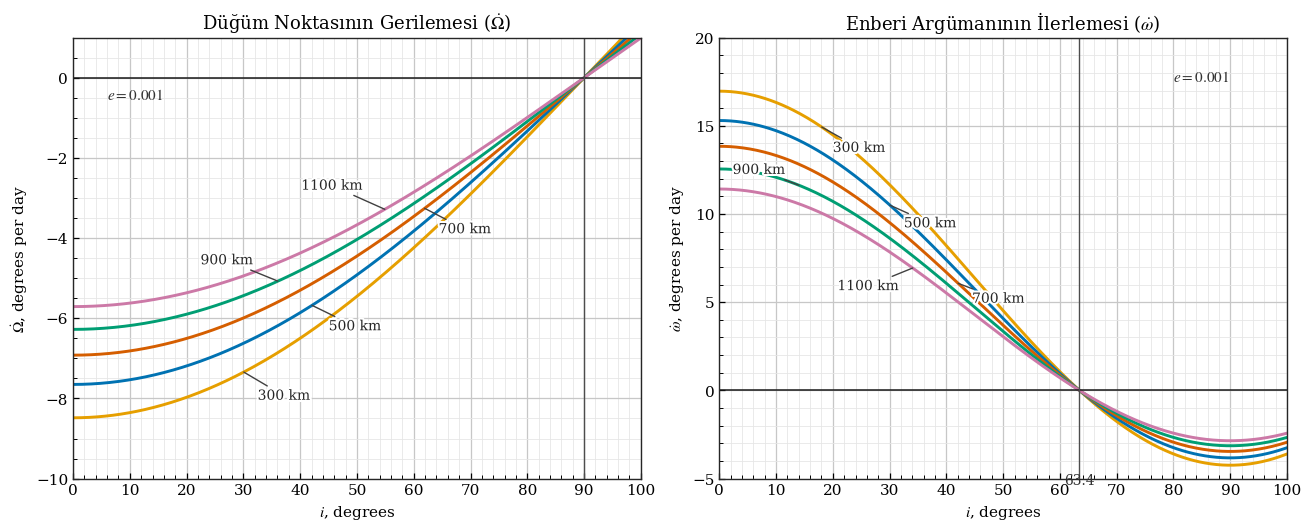
\includegraphics[width=1\linewidth]{Resimler/Dünya Modeli/RAAN ve Perigee V2.png}
    \caption{$J_2$ pertürbasyonuna bağlı olarak Düğüm Noktasının Gerilemesi ($\dot{\Omega}$) ve Enberi Argümanının İlerlemesi ($\dot{\omega}$) hızlarının yörünge eğikliği ve irtifaya göre değişimi ($e=0.001$).}
    \label{fig:j2_perturbations}
\end{figure}

Şekil~\ref{fig:j2_perturbations} incelendiğinde \cite{curtis2020orbital}, bu etkinin irtifa ve eğiklik ile olan hassas ilişkisi net bir biçimde görülmektedir. Soldaki grafikte, Düğüm Noktasının Gerilemesi ($\dot{\Omega}$) eğiklik ($i$) arttıkça azalmakta ve kutupsal yörüngelerde ($i=90^\circ$) sıfıra inmektedir. Düşük irtifalarda (örneğin 300 km) bu sürüklenme etkisi, yüksek irtifalara kıyasla çok daha belirgindir; bu durum $\dot{\Omega} \propto a^{-3.5}$ bağımlılığının doğrudan bir sonucudur. Sağdaki grafikte ise Enberi Argümanının İlerlemesi ($\dot{\omega}$), $i \approx 63.4^\circ$ değerinde işaret değiştirmektedir. Bu nokta \textbf{kritik eğim} olarak bilinir ve apsis hattının dönmesini durdurmak için Molniya gibi özel yörüngelerde stratejik olarak kullanılır. Grafikler, görev tasarımcısına istenen yörünge düzlemi presesyonunu elde etmek için hangi irtifa-eğiklik kombinasyonunun seçilmesi gerektiği konusunda doğrudan bir rehber sunar.



% -------------------- Lagrange Gezegen Denklemleri --------------
\subsection{Lagrange Gezegen Denklemleri (LPE)}\label{subsec:J2_LPE}

GVE yaklaşımı bozucu ivmeyi (RTN bileşenleri) doğrudan kullanırken, LPE yaklaşımı bozucu fonksiyon $\mathcal{R}$ üzerinden ilerler. $J_2$ etkisi \textbf{korunumlu} (\emph{konservatif}) bir potansiyelden türediği için, $\langle\dot{\Omega}\rangle$ ve $\langle\dot{\omega}\rangle$ gibi seküler oranlar LPE ile GVE’ye alternatif bir yoldan ve aynı sonuçlarla elde edilebilir. Kuvvet/ivme bileşenleri üzerinden çalıştığı için GVE, pertürbasyonun yönünü ve fiziksel etkisini yorumlama açısından çoğu zaman daha sezgiseldir; buna karşılık \textbf{konservatif alanlarda} LPE, potansiyelin ortalaması $\bar{\mathcal{R}}$ üzerinden ilerleyerek seküler dinamiği \textbf{daha sistematik} ve daha kompakt bir biçimde kurma avantajı sağlar. Bu nedenle, yöntembilimsel bütünlük sağlamak ve iki yaklaşımın eşdeğerliğini göstermek amacıyla, önce GVE ile elde edilen seküler sonuçlar bu kez LPE kullanılarak yeniden türetilecektir.


\subsubsection*{(i) Ortalama bozucu fonksiyon $\bar{\mathcal R}_{J_2}$}
$J_2$ bozucu fonksiyonu
\[
\mathcal R_{J_2} \;=\; -\frac{\mu R_E^2 J_2}{2r^3}\,(3\sin^2\phi-1),
\qquad \sin\phi=\sin i\sin u
\]
olduğundan, yörünge ortalaması alındığında (kısa-periyot terimler elenerek)
\begin{equation}
\boxed{
\bar{\mathcal R}_{J_2}
\;\triangleq\; \big\langle \mathcal R_{J_2}\big\rangle
\;=\; -\frac{\mu R_E^2 J_2}{4a^3(1-e^2)^{3/2}}\big(1-3\cos^2 i\big)
}
\label{eq:Rbar_J2}
\end{equation}
elde edilir. Bu ifade yalnızca $(a,e,i)$’ye bağlıdır ve açı değişkenlerine bağlı olmadığı için
seküler problemde $a,e,i$ sabit kalırken $\Omega$ ve $\omega$ sürüklenir.

\subsubsection*{(ii) Ortalama Lagrange denklemleri ile $\langle\dot\Omega\rangle$ ve $\langle\dot\omega\rangle$}
Ortalama bozucu fonksiyon kullanıldığında (yani $\bar{\mathcal R}$ ile),
klasik LPE’nin düğüm hattı ve perigee için pratik seküler formları:
\begin{subequations}\label{eq:LPE_secular_forms}
\begin{align}
\big\langle \dot\Omega \big\rangle \;&=\;
\frac{1}{n a^2\sqrt{1-e^2}\,\sin i}\,
\frac{\partial \bar{\mathcal R}}{\partial i},
\label{eq:LPE_Om}\\[4pt]
\big\langle \dot\omega \big\rangle \;&=\;
\frac{\sqrt{1-e^2}}{n a^2 e}\,
\frac{\partial \bar{\mathcal R}}{\partial e}
\;-\;
\frac{\cos i}{n a^2\sqrt{1-e^2}\,\sin i}\,
\frac{\partial \bar{\mathcal R}}{\partial i}.
\label{eq:LPE_om}
\end{align}
\end{subequations}
Şimdi \eqref{eq:Rbar_J2} ifadesinin türevlerini alalım. Önce $i$ türevi:
\[
\frac{\partial \bar{\mathcal R}_{J_2}}{\partial i}
=
-\frac{\mu R_E^2 J_2}{4a^3(1-e^2)^{3/2}}\,
\frac{\partial}{\partial i}\big(1-3\cos^2 i\big)
=
-\frac{\mu R_E^2 J_2}{4a^3(1-e^2)^{3/2}}\,(6\cos i\sin i).
\]
Bunu \eqref{eq:LPE_Om} içine koyarsak
\[
\big\langle \dot\Omega \big\rangle
=
\frac{1}{n a^2\sqrt{1-e^2}\sin i}
\Bigg(
-\frac{3\mu R_E^2 J_2}{2a^3(1-e^2)^{3/2}}\cos i\sin i
\Bigg)
=
-\frac{3}{2}J_2\,n\Big(\frac{R_E}{p}\Big)^2\cos i
\]
bulunur ve bu, GVE sonucu \eqref{eq:Omega_secular_J2} ile aynıdır.

Benzer şekilde $e$ türevi yalnızca $(1-e^2)^{-3/2}$ faktöründen gelir:
\[
\frac{\partial}{\partial e}\Big[(1-e^2)^{-3/2}\Big]
=
\frac{3e}{(1-e^2)^{5/2}}.
\]
Dolayısıyla
\[
\frac{\partial \bar{\mathcal R}_{J_2}}{\partial e}
=
-\frac{\mu R_E^2 J_2}{4a^3}\,
\frac{3e}{(1-e^2)^{5/2}}\,(1-3\cos^2 i).
\]
Bunu \eqref{eq:LPE_om} içine yerleştirip sadeleştirdiğimizde
\[
\big\langle \dot\omega \big\rangle
=
\frac{3}{4}J_2\,n\Big(\frac{R_E}{p}\Big)^2\big(5\cos^2 i - 1\big)
\]
elde edilir; bu da GVE sonucu \eqref{eq:omega_secular_J2} ile birebir aynıdır.

\subsubsection*{(iii) Sonuç: iki yol, aynı seküler fizik}
Özetle, $J_2$ gibi konservatif zonal pertürbasyonlarda:
\begin{itemize} \item GVE yaklaşımı $\mathbf a_{J_2}$’yi RTN bileşenlerine ayırarak doğrudan eleman driftlerini verir.
\item LPE yaklaşımı $\bar{\mathcal R}_{J_2}$ üzerinden kısmi türevlerle aynı seküler oranları üretir.
\end{itemize}
Bu noktadan sonra özel yörüngeler altbölümünde,
Sun-synchronous tasarımında \eqref{eq:Omega_secular_J2},
Molniya/kritik eğimde ise \eqref{eq:omega_secular_J2} temel denklemler olarak kullanılacaktır.


% ----------------- Daha Yüksek Zonal Terimler ----------------
\subsection{$J_3$, $J_4$ ve Daha Yüksek Zonal Terimler}
\label{subsec:J3_J4}

$J_2$'nin en baskın zonal bileşen olduğunu belirtmiştik. Örneğin
$J_3$ katsayısı, $J_2$'ye kıyasla yaklaşık $10^{-3}$ mertebesinde daha küçüktür; benzer biçimde $J_4$ da yaklaşık olarak $J_3$'e göre bir mertebe daha zayıf olup $10^{-6}$ mertebesine iner. Bu nedenle $J_3$, $J_4$ ve daha yüksek dereceli zonal terimler,
$J_2$'ye kıyasla oldukça küçük katkılar verir.

Yüksek hassasiyet gerektirmeyen tahmini analizlerde, bu küçük terimlerin büyüklüğü çoğu zaman \textbf{Kaula kuralı} ile mertebe düzeyinde tahmin edilir. Kaula kuralı, küresel harmonik katsayılarının genliğinin dereceyle yaklaşık olarak $\ell^{-2}$ ölçeğinde azaldığını öngören \textbf{ampirik} bir yaklaşımdır. Bu bağlamda, zonal terimler için tipik bir mertebe tahmini

\begin{equation}
|J_\ell| \;\sim\; \frac{|J_2|}{\ell^2}
\qquad (\ell\ge 3)
\label{eq:kaula_zonal}
\end{equation}
şeklinde verilebilir.

Buna karşın, yüksek hassasiyetli yörünge hesaplarında $J_3$, $J_4$ ve daha yüksek dereceli terimlerin tahmin edilmesi yeterli değildir; bu katsayıların güvenilir bir jeopotansiyel modelinden (örn.\ EGM/GRACE tabanlı modeller) alınarak nokta atışı şekilde
kullanılması gerekir. Çünkü Kaula kuralı yalnızca katsayıların \textbf{tipik büyüklük mertebesini} yakalar; yerel kütle anomalilerinin (dağlar, yoğunluk farkları vb.) uzaysal dağılımını ve bunların faz bilgisini temsil etmez. Dolayısıyla daha yüksek dereceli zonal terimler, Dünya'nın küresel şekline daha ince düzeltmeler ekleyerek özellikle uzun süreli propagasyonda
ve hassas görev analizlerinde uydunun izlediği yörüngeyi anlamlı ölçüde etkileyebilir. 

Genel olarak yüksek zonal terimlerin fiziksel anlamını ve yörünge elemanlarına yansımasını şöyle özetleyebiliriz:

\begin{itemize}
\item \textbf{$J_3$ (armut/pear-shape bileşeni):}
$J_3$ tek dereceli bir zonal terim olduğundan, kuzey--güney yönünde \textbf{asimetrik} bir katkı karakteri taşır. Bu yüzden etkileri çoğu zaman tamamen seküler bir sürüklenmeden ziyade
\textbf{uzun periyotlu} (long-period) salınımlar şeklinde görülür.
Özellikle eksantriklik $e$ ve perigee argümanı $\omega$ gibi elemanlarda, yörüngenin perigeesinin enleme göre konumlanmasına bağlı olarak yavaş değişimler/oscillasyonlar üretebilir.
(Çok küçük $e$’li neredeyse dairesel yörüngelerde bu etkinin gözlenmesi zorlaşır.)

\item \textbf{$J_4$ ve çift dereceli daha yüksek zonaller ($J_6,\dots$):}
Bu terimler, $J_2$’nin temsil ettiği ana basıklık üzerine
daha ince global şekil düzeltmeleri ekler. Etkileri genellikle $J_2$’ye göre daha küçük olsa da, \textbf{hassas yörünge propagasyonu} gerektiğinde (yüksek doğruluklu LEO görevleri,
uzun süreli yayılım, hassas yer izleme/ground-track gereksinimleri) ihmal edilemeyecek seviyeye çıkabilir.
Özellikle LEO’da, $J_2$ ile birlikte $J_4$ gibi terimler de $\Omega$ ve $\omega$ için ek precesyon bileşenleri ve elemanlarda daha karmaşık uzun periyot davranışları oluşturur.

\item \textbf{$J_5$ gibi tek dereceli daha yüksek zonaller ($J_5,J_7,\dots$):}
$J_3$’e benzer biçimde, kuzey--güney asimetri karakterli daha ince katkıları temsil ederler. Uygulamada çoğu zaman $J_2$ ve $J_4$ kadar ilk sırada yer almazlar; ancak uzun süreli propagasyon ve yüksek doğruluk hedeflerinde, özellikle belirli eğiklik/eksantriklik kombinasyonlarında uzun periyotlu etkiler biriktirebilirler.
\end{itemize}

\noindent
\textbf{Kısacası:}
Kaba görev analizlerinde çoğu zaman $J_2$ terimi baskındır ve yeterli bir ilk yaklaşım sunar; ancak hassasiyet gereksinimi arttıkça $J_3$, $J_4$ ve daha yüksek dereceli terimler
(başka bir deyişle model derecesi yükseldikçe) ihmal edilemeyecek düzeye gelir. Bu nedenle hangi zonal terimlerin modele dahil edileceği, \textbf{irtifa}, \textbf{zaman ufku} ve \textbf{istenen doğruluk} ile birlikte; gerekirse Kaula kuralı ile yalnızca mertebe düzeyinde bir ön değerlendirme yapılıp,
nihai analizde güvenilir jeopotansiyel katsayıları kullanılarak belirlenmelidir.




% =================== Özel Yörüngeler ====================
\newpage
\section{Özel Yörüngeler}
\label{sec:special_orbits}

Bu altbölümde, yerçekimi potansiyelinin düşük dereceli bileşenlerinin yörünge dinamiğinde neden bu kadar belirgin izler bıraktığına odaklanacağız. Bunun temel nedeni düşük dereceli terimler (özellikle zonaller), potansiyelin en büyük genlikli ve en geniş ölçekli sapmalarını taşır. Bu sapmalar her turda tekrar tekrar etki ettiği için, kısa zaman ölçeklerinde küçük görünen katkılar uzun vadede \textbf{birikimli} (\emph{seküler}) değişimlere dönüşebilir.

Bu çerçevede $J_2$ terimi, hem büyüklüğü hem de $\Omega$ (düğüm doğrusu) ve $\omega$ (apsis hattı / perigee argümanı) üzerinde ürettiği uzun dönemli, birikimli ortalama sürüklenmeler nedeniyle analizlerde birinci sıradadır. Özellikle $\Omega$ ve $\omega$’nun
ortalama precesyon hızları, görev tasarımında istenen yörünge geometrisini korumak veya istenen biçimde ayarlamak için birer kontrol parametresi gibi kullanılır. Aşağıda bu fikrin üç klasik yörünge ailesinde nasıl somutlaştığını görüyoruz.


% ---------------- Sun Synchronous -------------
\subsection*{2.4.1 \hspace{0.25em} Güneş-Eşzamanlı Yörüngeler (SSO)}
\label{subsec:sso}

Güneş-eşzamanlı yörüngelerde (Sun-Synchronous Orbit, SSO) amaç,
yörünge düzleminin uzaydaki yöneliminin (düğüm doğrusu, $\Omega$)
Güneş'in görünür yıllık hareketiyle \textbf{aynı ortalama açısal hızda}
dönmesini sağlamaktır.
Bu sayede uydu, aynı enlemden ardışık geçişlerinde yaklaşık aynı
\textbf{Yerel Güneş Zamanı} (Local Solar Time, LST) değerine sahip olur;
özellikle görüntüleme/uzaktan algılama görevlerinde aydınlatma koşulları
yıl boyunca daha \textbf{tutarlı} kalır.

Bu geometrik ilişki Şekil \ref{fig:sso_geometry}'de gösterilmiştir.
Düzlemin Güneş ile senkron kalması için düğüm presesyon hızı,
Dünya'nın Güneş etrafındaki ortalama açısal hızına eşitlenir:
\begin{equation}
\dot\Omega \;\approx\; \dot\Omega_{\odot}
\;\approx\; \frac{360^{\circ}}{365.25\ \text{gün}}
\;\approx\; 0.9856^{\circ}/\text{gün}.
\label{eq:sso_condition}
\end{equation}

\begin{figure}[h]
    \centering
    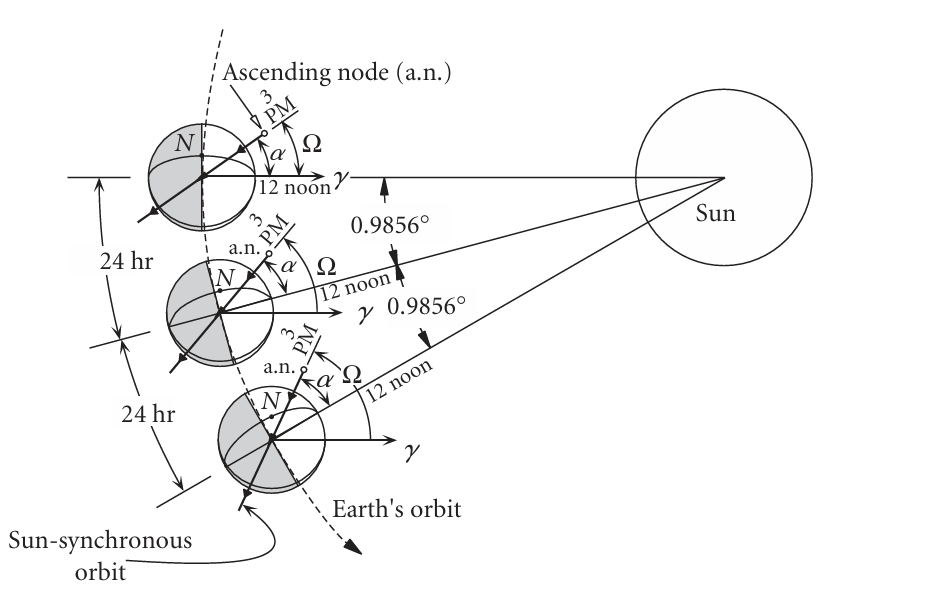
\includegraphics[width=0.85\linewidth]{Resimler/Dünya Modeli/SSO.png}
    \caption{Güneş-eşzamanlı yörüngenin geometrisi ve düğüm hattının Güneş ile senkron hareketi \cite{curtis2020orbital}.}
    \label{fig:sso_geometry}
\end{figure}

$J_2$ etkisi altında elde edilen seküler düğüm sürüklenmesi ifadesi \eqref{eq:Omega_secular_J2} dikkate alındığında,
\[
\big\langle \dot\Omega \big\rangle
\;=\; -\frac{3}{2}\,J_2\,n\Big(\frac{R_E}{p}\Big)^2\cos i,
\]

burada $n=\sqrt{\mu/a^3}$ ortalama hareketi, $p=a(1-e^2)$ ise yarı-parametreyi temsil eder.
Dolayısıyla $\langle \dot\Omega\rangle$ temel olarak $a$ (hem $n$ hem $p$ üzerinden), $e$ ( $p$ üzerinden)
ve $i$ ( $\cos i$ üzerinden) ile belirlenir.

SSO tasarımında hedef, düğüm hattının yıllık Güneş hareketine kilitlenmesidir; bu nedenle \eqref{eq:Omega_secular_J2} ile \eqref{eq:sso_condition} birlikte kullanılarak tasarım bağıntısı elde edilir:
\begin{equation}
\cos i
\;=\;
-\frac{2}{3}\;
\frac{\dot\Omega_{\odot}}{J_2\,n}\;
\Big(\frac{p}{R_E}\Big)^2.
\label{eq:SSO_design_relation}
\end{equation}

\begin{itemize}
    \item \textbf{İrtifa--eğim bağımlılığı:}
    $e\simeq 0$ için $p\simeq a$ ve $n\propto a^{-3/2}$ olduğundan,
    \eqref{eq:SSO_design_relation} yaklaşık olarak $\cos i \propto a^{7/2}$ ölçeğinde değişir.
    Bu yüzden pratikte bir \textbf{irtifa bandı} seçilir ve buna karşılık gelen $i$ belirlenir.

    \item \textbf{Retrograd gerekliliği:}
    \eqref{eq:Omega_secular_J2}'daki eksi işareti nedeniyle hedeflenen işaret için
    $\cos i<0$ olmalıdır; dolayısıyla SSO'lar tipik olarak
    $90^{\circ}<i<180^{\circ}$ aralığında \textbf{retrograd} seçilir.
\end{itemize}

Pratikte SSO'lar çoğunlukla düşük eksantriklikli LEO yörüngeleridir ($e\approx 0$).
Ayrıca atmosferik sürükleme zamanla $a$'yı azalttığından,
$\langle \dot\Omega\rangle$ da yavaşça değişebilir; hassas LST korunumu için
operasyonel düzeltmeler gerekebilir.

Sonuç olarak SSO, $J_2$ kaynaklı düğüm presesyonunun bir ``hata'' değil,
doğru seçilmiş $(a,i,e)$ ile görev gereksinimini sağlayan
\textbf{bilinçli bir tasarım aracı} olarak kullanıldığı klasik bir örnektir.




% --------------- Molniya Yörüngeleri -----------------
\subsection*{2.4.2 \hspace{0.25em} Molniya Yörüngeleri}
\label{subsec:molniya}

Molniya tipi yörüngeler, yüksek dışmerkezlikli ve yüksek eğimli (eliptik) yörüngelerdir.
Bu sınıfta temel amaç, enöte civarındaki uzun kalış bölgesinin (dolayısıyla kapsama geometrisinin)
zamanla yer değiştirmemesidir. Bu nedenle tasarımda özellikle apsis hattının yönelimi ve
\textbf{enberi argümanının} $\omega$ seküler sürüklenmesi kritik hale gelir.

\begin{tcolorbox}[
    colback=blue!8!white,
    colframe=blue!35!black,
    boxrule=0.6pt,
    arc=2mm,
    left=4pt,
    right=4pt,
    top=4pt,
    bottom=4pt,
    title=\small\textbf{Tarihsel ve Operasyonel Motivasyon}
]
Rus fırlatma sahalarının büyük bölümü $45^\circ$ enleminin üzerindedir
(kuzeydeki Plesetsk $\sim62.8^\circ$N).
Bu enlemlerden jeostasyoner yörüngeye (GEO) doğrudan erişim,
Ekvator düzlemiyle olan eğim farkı nedeniyle genellikle \textbf{pahalı bir düzlem değiştirme} (\emph{plane change}) manevrası gerektirir. Bu tür bir düzlem değiştirme manevrasının yaklaşık hız gereksinimi
\[
\Delta V_{\text{pc}} \;\approx\; 2\,V\,\sin\!\Big(\frac{\Delta i}{2}\Big),
\]
şeklinde ifade edilebilir; burada $V$ yörünge hızı, $\Delta i$ ise gerekli eğim değişimini temsil eder.
Yüksek irtifa ve hızlarda bu maliyet hızla büyür. Öte yandan GEO uyduları yüksek kuzey enlemlerini düşük yükselim açısıyla gözlediği için, kapsama geometrisi ve link bütçesi dezavantajlı hale gelir. Bu nedenle Sovyet/Rus haberleşme mimarisinde, 12 saat periyotlu ve yüksek eliptik (HEO) yörüngeler, yüksek enlemler üzerinde uzun süreli görünürlük sağlamak için etkili bir çözüm olarak öne çıkmıştır \cite{curtis2020orbital}.
\end{tcolorbox}


\eqref{eq:omega_secular_J2} ifadesi hatırlanırsa, $J_2$ kaynaklı ortalama enberi precesyonu
\begin{align*}
\big\langle \dot\omega \big\rangle
\;=\; \frac{3}{4}\,J_2\,n\Big(\frac{R_E}{p}\Big)^2\big(5\cos^2 i - 1\big)
\end{align*}
şeklindedir. Molniya tasarımında hedef, enöte bölgesinin seçilen yarımkürede kararlı kalması için
$\langle\dot\omega\rangle$ değerini sıfıra (veya sıfıra yakın) indirmektir. Bu da
\begin{equation}
5\cos^2 i-1=0
\quad\Longrightarrow\quad
i \approx 63.435^\circ \ \ (\text{veya }116.565^\circ)
\label{eq:critical_inclination}
\end{equation}
koşulunu verir. Bu değer \textbf{kritik eğim} olarak bilinir; kritik eğimde $J_2$ etkisinin $\omega$ üzerindeki seküler (ortalama) bileşeni bastırılır ve apsis hattının yönelimi uzun vadede daha kararlı hale gelir. Bu nedenle Molniya tasarımlarında eğim çoğunlukla kritik eğim civarında seçilir ($i \approx 63.435^\circ$); böylece apsis hattının uzun vadeli yönelimi korunarak enöte bölgesindeki kapsama geometrisi kararlı tutulur.


\begin{figure}[h]
    \centering
    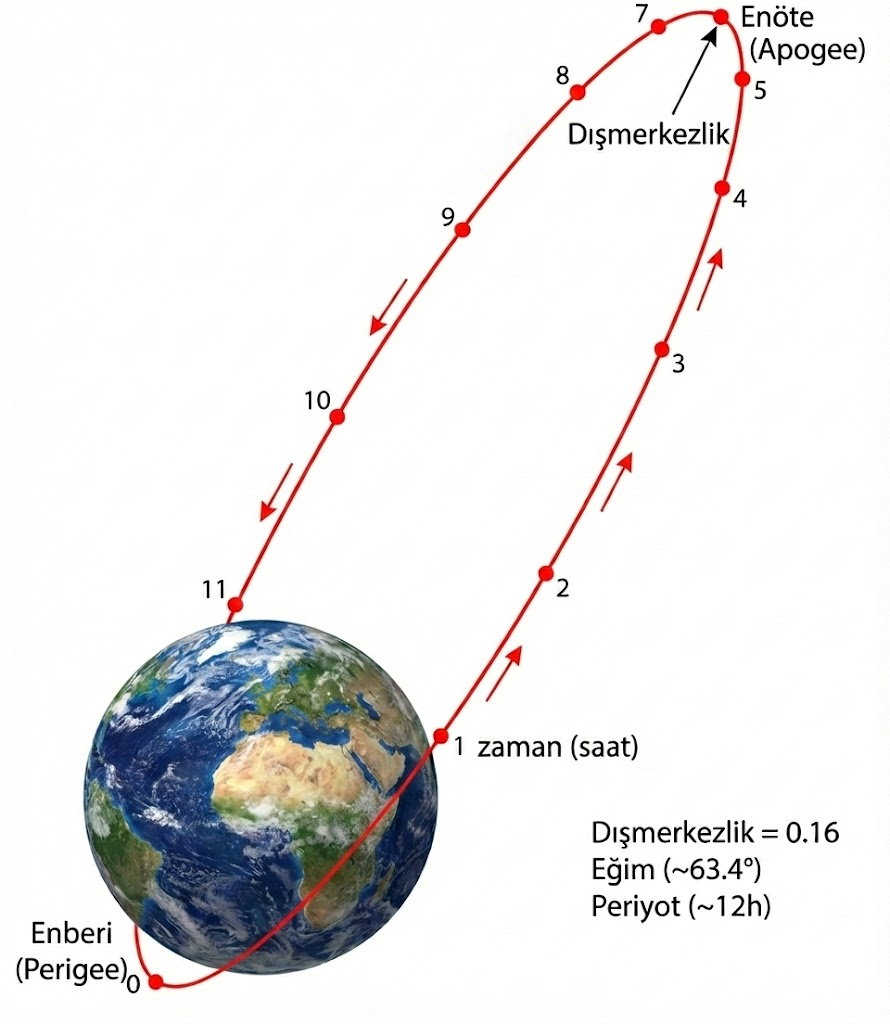
\includegraphics[width=0.5\linewidth]{Resimler/Dünya Modeli/Molniya Yörüngesi.png}
    \caption{Molniya tipi 12 saatlik eliptik yörüngede uydunun yörünge boyunca konumu. Enöte civarında hızın azalması nedeniyle zaman işaretleri sıklaşır; bu, uydunun periyodun büyük kısmını enöte yakınında geçirerek yüksek enlemlere uzun süreli kapsama sağlamasının görsel bir göstergesidir.}
    \label{fig:molniya_orbit}
\end{figure}

Şekil~\ref{fig:molniya_orbit}, kapsama avantajının dinamik nedenini görselleştirir:
uydu enöte civarında daha yavaş ilerlediği için eşit zaman aralıklarıyla işaretlenen konum noktaları
enöte yakınında daha sık, enberi yakınında ise daha seyrek görünür.
Bu dağılım Kepler’in ikinci yasasının doğrudan sonucudur ve uydunun periyodun önemli bir kısmını
enöte çevresinde geçirdiğini gösterir. Ayrıca $T\simeq 12$ saat seçimi,
yer izi ve yer istasyonu geometrisi açısından günlük tekrar eden bir örüntü sağlayarak operasyonel planlamayı kolaylaştırır.


% ---------------- Tundra Yörüngeleri-------------
\newpage
\subsection*{2.4.3 \hspace{0.25em} Tundra Yörüngeleri}
\label{subsec:tundra}

Tundra yörüngeleri, Molniya’daki temel prensibi (apsis hattını kararlı tutma ve enöteyi
istenen yarımküreye ``kilitleme'') \textbf{yaklaşık 1 yıldız günü (sidereal day) periyot}
çevresinde uygular. Bu sınıf, özellikle \textbf{yüksek enlemlere hizmet veren haberleşme}
görevlerinde, jeostasyoner yörüngelerin yüksek enlemlerdeki düşük yükselim açısı
dezavantajını azaltmak amacıyla geliştirilmiş yüksek eliptik
\emph{jeosenkron} (HEO--GSO) yörüngelerdir.

Tundra tasarımının merkezinde \textbf{apogee dwell} olgusu yer alır:
uydu enöte civarında belirgin biçimde yavaşladığı için yörünge periyodunun büyük bir
kısmını seçilen coğrafi bölge üzerinde geçirir.
Periyot bir güne yaklaştığında bu uzun kalış her gün yaklaşık aynı yerel zamanlarda
tekrar eder; bu durum yer istasyonu planlamasını ve görünürlük sürekliliğini
operasyonel açıdan avantajlı hâle getirir.

Dinamik açıdan Tundra yörüngeleri iki temel koşula dayanır:
\begin{itemize}
    \item \textbf{Periyot (jeosenkronluk):}
    Periyot $T \approx 1$ yıldız günü olacak şekilde yarı-büyük eksen $a$ seçilir.
    Bu seçim, yörüngenin Dünya’ya göre günlük tekrar eden bir yer izi üretmesini sağlar.

    \item \textbf{Eğim (J$_2$ ile apsis kararlılığı):}
    $J_2$ kaynaklı seküler apsis sürüklenmesini azaltmak için eğim çoğunluklakla
    \textbf{kritik eğime} yakın seçilir ($i \approx 63.4^\circ$ veya tamamlayanı).
    Böylece $\dot{\omega}$’nun seküler bileşeni bastırılarak apsis hattının
    uzaydaki yönelimi uzun vadede korunur.
\end{itemize}

Pratik uygulamalarda Tundra yörüngeleri \textbf{orta--yüksek dışmerkezlik} ile tasarlanır;
tipik olarak $e \sim 0.2{-}0.3$ aralığı, enöte civarında yeterli ``loiter'' süresi
sağlarken kapsama geometrisini de operasyonel olarak elverişli kılar.
Bu sayede uydu, seçilen boylam/enlem bandı üzerinde
\textbf{yüksek yükselim açısıyla} uzun süre görünür kalabilir.

\begin{figure}[h]
    \centering
    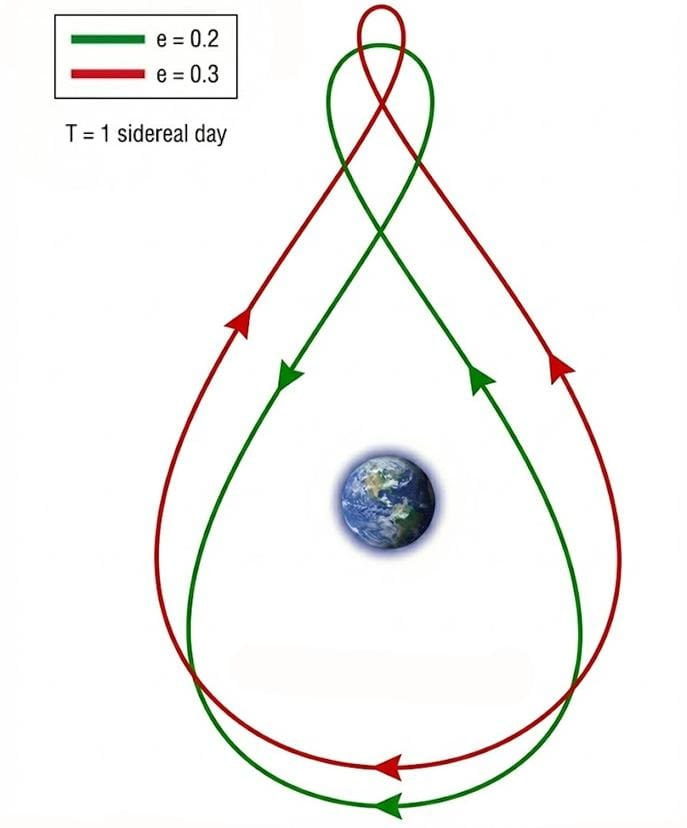
\includegraphics[width=0.5\linewidth]{Resimler/Dünya Modeli/Tundra.jpeg}
    \caption{Dünya ile dönen (Earth-fixed) referans çerçevesinde,
    farklı dışmerkezliklere ($e=0.2$ ve $e=0.3$) sahip Tundra yörüngelerinin
    yer izi (analemma) görünümü.}
    \label{fig:tundra_analemma}
\end{figure}

Şekil~\ref{fig:tundra_analemma}, iki farklı dışmerkezlik değerine sahip Tundra
yörüngesinin Dünya’ya göre algılanan yer izini göstermektedir.
Dünya ile dönen (\emph{Earth-fixed}) bir referans çerçevesinde,
yörünge kapalı bir ``8'' (analemma) biçimi oluşturur.
Bu şekil, Dünya’nın günlük dönüşü ile yörüngenin jeosenkron periyodunun
birlikte etkisinin doğrudan sonucudur.
Buna karşılık, eylemsiz (\emph{Earth-centered inertial}) referans çerçevesinde
Tundra yörüngesi basit bir elips olarak tanımlanır.

Şekilden de görüldüğü üzere, dışmerkezlik arttıkça enöte civarındaki
\textbf{apogee dwell} süresi artmakta ve analemmanın ilgili yarımküredeki
halkası daha baskın hâle gelmektedir.
Bu durum, Tundra yörüngelerinin belirli bir coğrafi bölge üzerinde
uzun süreli ve yüksek yükselimli görünürlük sağlamasının
geometrik ve dinamik temelini açıkça ortaya koyar.

Sonuç olarak Tundra yörüngeleri, $J_2$ kaynaklı apsis sürüklenmesini
\emph{tasarım lehine} kullanarak,
jeosenkron periyot ile enöte kalışını birleştiren ve
belirli bir bölge üzerinde sürekliliğe yakın kapsama sağlamaya odaklanan
özel bir yüksek eliptik yörünge ailesidir.


% ------------------ Özet -------------------
\subsection*{2.4.4 \hspace{0.25em} Özet}
Güneş-eşzamanlı, Molniya ve Tundra örnekleri, $J_2$ kaynaklı seküler sürüklenmelerin yalnızca
``istenmeyen pertürbasyonlar'' olmadığını gösterir. Uygun $(a,e,i)$ seçimiyle
$\Omega$ ve $\omega$ üzerindeki ortalama precesyonlar \textbf{hedeflenebilir} veya
\textbf{bastırılabilir}; böylece görev gereksinimlerine uyumlu \textbf{özel yörünge} aileleri
tasarlanır. Bu bakımdan $J_2$, pertürbasyon modellemesinin ötesinde,
yörünge geometrisini uzun vadede yönlendiren bir \textbf{tasarım parametresi} gibi davranır.
Aşağıdaki tabloda bu üç yörünge ailesinin temel özellikleri karşılaştırılmıştır.

\medskip
\begin{table}[h]
\centering
\captionsetup{skip=6pt}
\renewcommand{\arraystretch}{1.25}
\setlength{\tabcolsep}{6pt}
\begin{tabular}{p{2.6cm} p{3.4cm} p{3.6cm} p{5.2cm}}
\hline
\textbf{Yörünge} &
\textbf{Ana hedef} &
\textbf{$J_2$ ile kurulan şart} &
\textbf{Tipik seçimler ve sonuç} \\
\hline
Güneş-Eşzamanlı (SSO) &
Yerel Güneş Zamanını (LST) yaklaşık sabit tutmak &
Düğüm precesyonu hedeflenir:
$\langle\dot\Omega\rangle \approx \dot\Omega_{\odot}$ &
LEO, düşük $e$; retrograd eğim ($i>90^\circ$).
Yıl boyunca benzer aydınlatma koşulları. \\
\hline
Molniya (HEO) &
Yüksek enlemlerde uzun süreli kapsama (enöte loiter) &
Apsis sürüklenmesi bastırılır:
kritik eğimde $\langle\dot\omega\rangle \approx 0$ &
$T\approx 12$ saat; yüksek $e$;
$i\approx 63.4^\circ$ (veya $116.6^\circ$).
Enöte civarında belirgin ``dwell'' süresi. \\
\hline
Tundra (HEO--GSO) &
Belirli bir boylam bölgesi üzerinde günlük tekrar eden uzun görünürlük &
$\langle\dot\omega\rangle$ azaltılır (kritik eğim civarı) ve enöte yönelimi korunur &
$T\approx 1$ yıldız günü; $e\sim 0.2{-}0.3$;
$i$ kritik eğime yakın.
Earth-fixed çerçevede analemma (``8'') yer izi. \\
\hline
\end{tabular}
\caption{SSO, Molniya ve Tundra yörüngelerinin $J_2$ ile ilişkili tasarım hedefleri ve tipik özellikleri.}
\label{tab:special_orbits_summary}
\end{table}




% ============== Potansiyel Ölçümleri ve Tarihçesi ===============
\newpage
\section{Potansiyel Ölçümleri ve Tarihçesi}
\label{sec:measurements_history_estimation}

Şimdiye kadar, yerçekimi potansiyelinin küresel harmonikler cinsinden nasıl temsil edildiğini gördük. Ancak Dünya özelinde bu katsayılara duyulan gereksinimin hangi fiziksel ve tarihsel nedenlerle ortaya çıktığı açıklığa kavuşturulmalıdır.
Bu bağlamda, \eqref{eq:earth_potential} denkleminde yer alan
$\bar C_{\ell,m}$ ve $\bar S_{\ell,m}$ katsayılarının nasıl bulunduğu incelenecektir.


% --------------- Modellerin Tarihçesi ------------
\subsection{Dünya Yerçekimi Modellerinin Tarihçesi}
\label{subsec:history_short}

Küresel yerçekimi modellerinin gelişimi, insanlığın yapay uyduları yörüngeye yerleştirmesiyle
doğrudan ivme kazanmıştır. Erken dönem uyduların yörüngelerinde gözlenen beklenmedik
sapmalar, Dünya’nın kütle dağılımının basit bir küresel modelle açıklanamayacağını ortaya koymuştur.
Ölçüm teknikleri ve izleme hassasiyeti geliştikçe, yalnızca düşük dereceli bileşenler değil,
daha ince uzaysal ayrıntılar ve hatta zamanla değişen kütle etkileri de görünür hale gelmiştir.

\begin{itemize}
\item \textbf{1957--1960’lar (ilk yapay uydular):}
Sputnik ve onu izleyen erken dönem uyduların yörüngelerinde gözlenen düğüm ve apsis sürüklenmeleri, yerçekimi alanındaki düşük dereceli zonal terimlerin (özellikle $J_2$) baskın rolünü açıkça ortaya koydu. Bu dönemde Dünya’nın basıklığı, ilk kez yalnızca jeodezik ölçümlerle değil, doğrudan yörünge dinamiği üzerinden nicel olarak doğrulanmış oldu.

\item \textbf{1970’ler ve LAGEOS (1976):}
LAGEOS uydularının lazerle menzillenmesi (SLR), yörünge konumunun milimetre mertebesinde izlenmesini mümkün kıldı. Atmosferik sürüklemenin ihmal edilebilir olduğu bu yüksek irtifa
uyduları, düşük dereceli ve uzun dalga boylu yerçekimi bileşenleri için son derece güvenilir referanslar sundu ve küresel modellerin temelini sağlamlaştırdı.

\item \textbf{2000 ve CHAMP:}
CHAMP göreviyle birlikte GNSS/GPS tabanlı hassas yörünge belirleme teknikleri olgunlaştı. Bu sayede yalnızca düşük dereceler değil, orta dereceli harmonik bileşenler de daha güvenilir biçimde çözümlenebildi. CHAMP, dinamik uydu izleme ile gravite modellemenin modern çağına geçişte kritik bir ara basamak olarak kabul edilir.

\item \textbf{2002 ve GRACE:}
GRACE görevi, iki uydu arasındaki bağıl mesafedeki mikrometre düzeyindeki değişimleri ölçerek yerçekimi alanını benzeri görülmemiş bir hassasiyetle haritaladı. Bu yaklaşım, yerçekimi alanının yalnızca statik bir nicelik olmadığını; buz tabakaları, yeraltı suyu, okyanus ve kara kütle değişimleri nedeniyle
\textbf{zamansal olarak değiştiğini} doğrudan gözler önüne serdi.

\item \textbf{2009 ve GOCE:}
GOCE uydusu üzerindeki gradiyometre, yerçekimi ivmesinin uzaysal türevlerini doğrudan ölçerek statik alanın kısa dalga boylu (yüksek dereceli) ayrıntılarını büyük ölçüde iyileştirdi.
Bunun sonucunda jeoit modelleri daha keskin, daha düzgün ve daha yüksek çözünürlüklü hale geldi; özellikle bölgesel jeodezi ve okyanus dinamiği uygulamaları önemli kazanımlar elde etti.

\item \textbf{2018 ve GRACE-FO:}
GRACE-FO görevi, GRACE ile başlatılan zamansal yerçekimi gözlemlerini sürdürerek uzun dönemli eğilimlerin (buz erimesi, su bütçesi değişimleri gibi) daha güvenilir biçimde izlenmesini sağladı. Lazer interferometre gibi yeni teknolojilerle ölçüm hassasiyeti daha da artırıldı ve zamansal gravite gözlemlerinin sürekliliği garanti altına alındı.
\end{itemize}

\medskip
\noindent
\textbf{Bugün gelinen nokta:}
Günümüzde Dünya yerçekimi alanı, düşük dereceli zonal terimlerden
yüksek dereceli ve zamana bağlı bileşenlere kadar geniş bir yelpazede yüksek doğrulukla modellenebilmektedir. EGM2008, EIGEN, ITSG ve benzeri modern jeopotansiyel modelleri, SLR, GNSS, GRACE/GRACE-FO, GOCE ve altimetri verilerinin çoklu veri birleşimiyle üretilmekte; böylece hem statik alanın ince
uzaysal ayrıntıları hem de zamansal kütle değişimleri güvenilir biçimde temsil edilebilmektedir. Bu gelişmeler, yalnızca yörünge mekaniği ve görev tasarımı açısından değil, iklim değişikliği, su kaynakları, buz tabakalarının evrimi ve jeodinamik süreçlerin izlenmesi açısından da yerçekimi modellerini vazgeçilmez
bir bilimsel araç haline getirmiştir.

% ------------------- EGM Ailesi -----------------
\subsection*{EGM ailesi ve çözünürlük seviyeleri}
\label{subsec:EGM_family}

EGM (Earth Gravitational Model) ailesi gibi küresel yerçekimi modelleri,
$\bar C_{\ell, m}, \bar S_{\ell, m}$ küresel harmonik katsayılarının standartlaştırılmış bir ``kataloğu'' olarak yayımlanır. Bir modelin uzaysal ayrıntı kapasitesi çoğu zaman
\textbf{maksimum derece ve mertebe} ile özetlenir:
\[
\ell_{\max} = m_{\max},
\]
yani potansiyel açılımının hangi dereceye kadar genişletildiği.
Genel olarak $\ell_{\max}$ büyüdükçe model,
Dünya üzerindeki daha kısa dalga boylu (daha küçük ölçekli)
kütle ve jeoit yapılarının temsilini mümkün kılar.

EGM ailesindeki başlıca modeller ve derece seviyeleri şu şekildedir:
\begin{itemize}
\item \textbf{EGM84:} $\ell_{\max}=180$,
\item \textbf{EGM96:} $\ell_{\max}=360$,
\item \textbf{EGM2008:} $\ell_{\max}=2160$
(Bölgesel uzatmalarla daha yüksek dereceler).
\end{itemize}

Pratik açıdan model derecesinin anlamı iki temel noktada ortaya çıkar:

\begin{itemize}
\item \textbf{Derece--uzaysal ölçek ilişkisi:}
Küresel harmoniklerin temsil ettiği karakteristik yatay dalga boyu,
yaklaşık olarak
\[
\lambda \sim \frac{2\pi R_E}{\ell}
\]
ile ölçeklenir.
Dolayısıyla $\ell_{\max}$ arttıkça modelin yatay çözünürlüğü artar.
Ancak bu artış, her coğrafi bölgede eşit veri kalitesi olduğu anlamına gelmez;
veri yoğunluğu zayıf alanlarda yüksek dereceli terimler
daha belirsiz olabilir.

\item \textbf{İrtifa ve sönüm etkisi:}
Yüksek dereceli terimlerin katkısı,
uydu irtifası arttıkça $(R_E/r)^{\ell}$ faktörü nedeniyle hızla zayıflar.
Bu nedenle alçak yörüngelerde (özellikle LEO)
yüksek dereceli terimler anlamlı hale gelirken,
yüksek irtifalarda düşük dereceli bileşenler baskın kalır.
\end{itemize}

Buna ek olarak, derece yükseldikçe tahmin edilmesi gereken katsayı sayısı
yaklaşık olarak $(\ell_{\max}+1)^2$ ile artar.
Bu durum daha fazla ve daha çeşitli gözlem verisi gerektirir;
ayrıca ölçüm gürültüsünün yüksek derecelerde baskın hale gelmemesi için
kestirim sürecinde düzenlileştirme (regularizasyon),
a priori bilgi ve kalite kontrol adımları kritik rol oynar.

Sonuç olarak uygulamada model seçimi,
yalnızca ``en büyük $\ell_{\max}$ en iyidir'' anlayışıyla yapılmaz.
Hedeflenen irtifa, görev süresi ve istenen doğruluk düzeyine bağlı olarak,
tam model yerine uygun bir dereceye kadar
\emph{kesilmiş} (truncated) bir jeopotansiyel model kullanmak
çoğu zaman daha dengeli ve güvenilir bir yaklaşımdır.



% ----------------- C ve S hesaplama -------------
\section{$\bar C_{\ell,m},\bar S_{\ell,m}$ katsayıları nasıl kestirilir?}
\label{sec:how_CS_estimated}

Tarihsel gelişim incelendikten sonra, bu bölümde
$\bar C_{\ell,m}$ ve $\bar S_{\ell,m}$ küresel harmonik katsayılarının günümüzde hangi ölçüm türlerine dayalı olarak ve hangi sayısal yöntemlerle kestirildiği ele alınmaktadır.
Önce yerçekimi alanına duyarlı başlıca gözlem kaynakları özetlenecek, ardından bu gözlemlerin dinamik yörünge modelleriyle birleştirilerek katsayıların ters problem çerçevesinde nasıl hesaplandığı açıklanacaktır.


\subsection{Ölçüm Yöntemleri}
Başlıca veri kaynakları şunlardır:

\begin{itemize}
\item \textbf{Yer temelli gravite ölçümleri:}
Gravimetre ölçümlerinden elde edilen $g$ anomalileri ve bunlardan türetilen jeoit/gravite alan ürünleri, özellikle karasal bölgelerde bölgesel ayrıntılara güçlü katkı sağlar. Yer istasyonlarının iyi tanımlı geometrisi önemli bir avantajdır; ancak okyanuslar, erişimi zor alanlar ve düzensiz istasyon dağılımı nedeniyle küresel kapsam sınırlı kalabilir.

\item \textbf{SLR (Satellite Laser Ranging):}
Uyduya lazer menzili ölçülerek yörünge çok yüksek doğrulukla bağlanır. LAGEOS benzeri uydular sayesinde düşük dereceli bileşenler (uzun dalga boyu; özellikle $J_2$ ve yakın terimler) üzerinde son derece güçlü bir kısıt sağlanır. Atmosferik sürüklemenin ihmal edilebilir olduğu yüksek irtifa SLR uyduları,
``temiz dinamik'' yörünge verisi sunmaları nedeniyle temel referans veri kaynağıdır.

\item \textbf{GNSS/Doppler izleme:}
GNSS (GPS, Galileo vb.) alıcıları ile Doppler ve menzil türü izleme verileri, uydunun konum ve hızının hassas belirlenmesini sağlar. Bu sayede yörünge üzerindeki küçük ivme farkları daha net ortaya çıkar ve küresel harmonik katsayılarının kestirimi güçlenir. Uygulamada bu veri türü çoğu zaman hassas yörünge belirleme (POD) sürecinin ana girdisidir.

\item \textbf{Uydu--uydu izleme (GRACE/GRACE-FO):}
İki uydu arasındaki menzil değişimi ve menzil hızı (K/Ka-band ya da lazer interferometresi) ölçülür. Bu ölçümler yerçekimi alanının orta dalga boylu yapıları için son derece hassastır.
En önemli avantajı, yalnızca statik alanı değil; su döngüsü, buz kütlesi ve yeraltı suyu gibi \textbf{zamansal kütle değişimlerini} aylık hatta haftalık ölçeklerde izleyebilmesidir.

\item \textbf{Gradiyometri (GOCE):}
Yerçekimi ivmesinin uzaysal türevleri (gradyanları) doğrudan ölçülür. Bu veri türü kısa dalga boylu (yüksek derece) statik alan ayrıntılarının belirlenmesinde son derece etkilidir ve yüksek çözünürlüklü jeoit modellerinin temel bileşenlerinden biridir. Bununla birlikte, düşük dereceler için tek başına yeterli olmadığından genellikle SLR ve GRACE verileriyle birlikte kullanılır.

\item \textbf{Altimetri:}
Radar altimetreleri ile deniz yüzeyi yüksekliği ölçülür.
Uzun dönemli ortalama deniz yüzeyi, dinamik okyanus etkileri ayrıştırıldıktan sonra
jeoitin dolaylı bir gözlemi olarak kullanılır.
Bu veri, özellikle okyanuslar üzerindeki orta ve kısa dalga boylu gravite bileşenlerine
katkı sağlar; ancak akıntılar, rüzgâr ve dalga etkilerinin modellenmesi kritik önemdedir.
\end{itemize}

Bu veri türlerinin her biri farklı uzaysal ve zamansal ölçeklere duyarlıdır: bazıları uzun dalga boyunu (düşük $\ell$), bazıları kısa dalga boyunu (yüksek $\ell$), bazıları ise zamanla değişen bileşenleri daha iyi temsil eder. Bu nedenle modern jeopotansiyel modelleri, farklı veri setlerini \textbf{çoklu veri birleşimi} (\emph{data fusion}) yaklaşımıyla bir araya getirir. Veri ağırlıkları, ölçüm gürültüsü ve model belirsizlikleri EKK çerçevesinde birlikte değerlendirilerek tutarlı ve yüksek doğruluklu bir katsayı kümesi elde edilir.


% ------------- Sayısal Hesaplama Yöntemi ---------------
\subsection{Sayısal Hesaplama Yöntemi}

$\bar C_{\ell,m}$ ve $\bar S_{\ell,m}$ katsayıları doğrudan ölçülebilen nicelikler değildir.
Bu katsayılar, yerçekimi alanının uydu yörüngeleri üzerindeki etkisini açıklayan
dinamik modeller ile çeşitli jeodezik gözlemleri ilişkilendiren bir
\textbf{ters problem} çözümü yoluyla kestirilir.
Uygulamada en yaygın yaklaşım, \textbf{En Küçük Kareler}
(EKK, \emph{least squares}) temelli parametre tahminidir.

Bu çerçevede amaç,
``katsayılar hangi değerleri alırsa, seçilen dinamik model gözlemleri en iyi açıklar?''
sorusuna yanıt bulmaktır.
Bu nedenle kestirim sürecinde yalnızca
$\bar C_{\ell,m}$ ve $\bar S_{\ell,m}$ değil;
uydu başlangıç koşulları, ölçüm sapmaları (\emph{bias}),
atmosferik sürükleme ve radyasyon basıncı gibi
yardımcı dinamik parametreler de birlikte ele alınır.

Tipik hesaplama süreci şu adımlardan oluşur:
öncelikle bir başlangıç jeopotansiyel modeli ve parametre kümesi seçilir;
hareket denklemleri bu parametrelerle sayısal olarak entegre edilerek
hesaplanan yörünge elde edilir.
Bu yörüngeden \textbf{hesap gözlemleri} üretilir ve gerçek ölçümlerle
karşılaştırılarak \textbf{artıklar} (\emph{residuals}) tanımlanır.
Problem doğrusal olmadığından, parametreler mevcut bir tahmin etrafında
lineerleştirilir ve çözüm iteratif olarak güncellenir.

Bu amaçla parametre vektörü
\[
\mathbf{x}=
\big[\bar{C}_{\ell m},\bar{S}_{\ell m}\big]^T,
\qquad
(2\le \ell\le \ell_{\max},\ 0\le m\le \ell)
\]
şeklinde tanımlansın.
Gözlemler genel olarak doğrusal olmayan bir modelle ifade edilir:
\begin{equation}
\mathbf{y}= \mathbf{h}(\mathbf{x})+\boldsymbol{\varepsilon},
\label{eq:obs_model}
\end{equation}
burada $\mathbf{h}(\mathbf{x})$ yörünge dinamiği ve ölçüm geometrisini içeren
gözlem modelini,
$\boldsymbol{\varepsilon}$ ise ölçüm gürültüsü ve modellenmemiş etkileri temsil eder.

Mevcut tahmin $\mathbf{x}_0$ etrafında yapılan lineerleştirme sonucunda
\begin{equation}
\Delta\mathbf{y}=\mathbf{A}\,\Delta\mathbf{x}+\boldsymbol{\varepsilon},
\qquad
\mathbf{A}=
\left.\frac{\partial \mathbf{h}}{\partial \mathbf{x}}\right|_{\mathbf{x}_0},
\label{eq:linearized}
\end{equation}
ifadesi elde edilir.
Burada $\mathbf{A}$ tasarım (Jakobiyen) matrisi olup,
her bir ölçümün her bir katsayıya duyarlılığını gösterir.

Farklı veri türlerinin doğruluk seviyeleri birbirinden farklı olduğundan,
kestirim süreci genellikle \textbf{ağırlıklı en küçük kareler} yaklaşımıyla yürütülür:
\begin{equation}
\min_{\Delta\mathbf{x}}
\left\|\mathbf{W}^{1/2}
\big(\mathbf{A}\Delta\mathbf{x}-\Delta\mathbf{y}\big)\right\|^2
\quad\Longrightarrow\quad
(\mathbf{A}^T\mathbf{W}\mathbf{A})\Delta\mathbf{x}
=\mathbf{A}^T\mathbf{W}\Delta\mathbf{y}.
\label{eq:wls_normal_eq}
\end{equation}
Burada $\mathbf{W}$ ağırlık matrisi olup,
ölçümlerin güvenilirliğini (gürültü seviyesini) temsil eder.

Her iterasyonda
$\mathbf{x}_{k+1}=\mathbf{x}_k+\Delta\mathbf{x}$
ile parametreler güncellenir.
Artıkların istatistiksel olarak tutarlı hale gelmesi ve
güncellemelerin ihmal edilebilir düzeye inmesiyle
çözümün yakınsadığı kabul edilir.
Sonuç olarak küresel harmonik katsayıları,
çoklu gözlem setleri ve dinamik modeller kullanılarak
\textbf{iteratif biçimde iyileştirilen}
bir ters çözüm süreciyle elde edilir.


% =============== Dinamik Yerçekimi Bozunumları =================
\newpage
\section{Dinamik Yerçekimi Bozunumları}
\label{sec:dynamic_gravity}

Bu noktaya kadar yerçekimi alanını zamandan bağımsız (\textbf{statik}) küresel harmonik bileşenler üzerinden ele aldık.
Bu yaklaşım pek çok mühendislik problemi için yeterli bir ilk mertebe model sağlasa da,
gerçek Dünya (ve Ay) yerçekimi alanı tam anlamıyla sabit değildir:
kütle dağılımı ve cisim şekli farklı fiziksel süreçler nedeniyle zamanla değişir ve
yerçekimi potansiyeline \textbf{zamana bağlı} bir bileşen ekler.
Bu çalışmada odak statik etkiler üzerinde kalsa da, dinamik etkilerin hangi koşullarda önem kazandığını
ve hangi hata mekanizmaları doğurabileceğini kavramsal düzeyde bilmek gerekir.
Bu nedenle bu bölüm, ayrıntılı türetimlere girmeden, dinamik yerçekimi bozunumlarını
\textbf{kaynakları, zaman ölçekleri ve yörünge dinamiğine etkileri} açısından kısa bir ``kontrol listesi'' olarak özetler.

Genel olarak potansiyel,
\begin{equation}
U(\mathbf{r},t) \;=\; U_{\text{statik}}(\mathbf{r}) \;+\; \Delta U(\mathbf{r},t),
\label{eq:U_static_plus_dynamic}
\end{equation}
şeklinde ayrıştırılabilir. Burada $\Delta U(\mathbf{r},t)$, kısa veya uzun zaman ölçeklerinde değişen
kütle yeniden-dağılımları ve deformasyonlar nedeniyle ortaya çıkan dinamik katkıları temsil eder.

Küresel harmonik bakış açısından bu durum, daha önce tanımladığımız \textbf{Stokes katsayıları}'nın  zamana bağlı hâle gelmesi şeklinde de ifade edilir:
\begin{equation}
C_{\ell,m}(t) = C_{\ell,m}^{(0)} + \Delta C_{\ell,m}(t),
\qquad
S_{\ell,m}(t) = S_{\ell,m}^{(0)} + \Delta S_{\ell,m}(t).
\label{eq:time_varying_coeffs}
\end{equation}
Özellikle düşük dereceli terimlerde (ör.\ $C_{2,0}$ benzeri) küçük değişimler bile uzun süreli propagasyonda
ölçülebilir farklar üretebilir.

Pratikte $\Delta C_{\ell,m}(t)$ ve $\Delta S_{\ell,m}(t)$ katkıları çoğunlukla (i) \textbf{katı cisim deformasyonu} (solid Earth/lunar tides), (ii) \textbf{akışkan kütle hareketleri} okyanus/atmosfer/hidrosfer) ve (iii) \textbf{üçüncü cisim etkileri} (Güneş ve diğer gökcisimleri) başlıkları altında incelenir. Katı cisim ve yükleme kaynaklı etkilerde, cismin elastik yanıtı doğrudan devreye girdiği için Love sayıları kullanılır.

% ------------------------------------------------------------
\subsection*{2.7.1 \hspace{0.25em} Love sayıları}
\label{subsec:love_numbers}

Katı cisim gelgitleri ve yükleme (loading) altında cismin elastik cevabı \textbf{Love sayıları} ile parametrik olarak ifade edilir:
\begin{itemize}
    \item $k_{\ell}$: \textbf{potansiyel Love sayısı} --- gelgit kaynaklı \textbf{potansiyel} değişimini ölçekler.
    \item $h_{\ell}$: \textbf{radyal yer değiştirme Love sayısı} --- \textbf{düşey} (radyal) deformasyonu temsil eder.
    \item $l_{\ell}$: \textbf{yatay yer değiştirme Love sayısı} --- \textbf{yatay} (teğetsel) deformasyonu temsil eder.
\end{itemize}

Love sayıları \textbf{dereceye bağlıdır} (ör.\ $\ell=2,3,\dots$) ve pratik uygulamalarda özellikle
$\ell=2$ bileşenleri (kuadrupol) dinamik düzeltmelerde baskındır.
Ayrıca \textbf{katı cisim gelgiti} ile \textbf{yükleme} (\emph{loading}) etkilerinin fiziksel kökeni farklı olduğundan,
literatürde çoğu zaman \textbf{body Love numbers} (solid tides için) ve \textbf{load Love numbers} (okyanus/atmosfer/hidrosfer yüklemesi için) ayrımı yapılır.

Bu çerçevede gelgit ve yükleme kaynaklı etkiler,
dış kaynaklı gelgit potansiyelinin cisim tarafından ne ölçüde ``yansıtılıp güçlendirildiğini''
($k_{\ell}$) ve deformasyon geometrisini ($h_{\ell}$, $l_{\ell}$) belirleyerek, sonuçta
$\Delta \bar{C}_{\ell,m}(t)$ ve $\Delta \bar{S}_{\ell,m}(t)$ türünden
zamana bağlı katsayı düzeltmelerine yansır (kullanılan normalizasyon tanımına göre $\bar{(\cdot)}$ yazımı değişebilir).

% ------------------------------------------------------------
\subsection*{2.7.2 \hspace{0.25em} Katı Cisim Gelgitleri (Solid Tides)}
\label{subsec:solid_tides}

Ay ve Güneş'in çekimi, Dünya üzerinde (Ay için ise Dünya'nun çekimi) bir \textbf{gelgit potansiyeli} oluşturarak
cisim gövdesinde elastik deformasyona neden olur. Bu deformasyon kütle dağılımını az da olsa değiştirir ve
yerçekimi alanına \textbf{zamanla değişen, çoğunlukla periyodik} bileşenler ekler.
Küresel harmonik yorumda bu etki, özellikle düşük dereceli katsayılara (ör.\ $C_{2,0}$ benzeri)
$\Delta C_{2,0}(t)$ türünden zamana bağlı düzeltmeler gelmesi şeklinde ifade edilir.
Bu düzeltmelerin \textbf{genliği ve fazı}, cismin elastik yanıtını temsil eden Love sayılarıyla ilişkilidir
(başta $k_{\ell}$; geometrik yer değiştirmeler için $h_{\ell}$ ve $l_{\ell}$).
Dolayısıyla solid tides, statik harmoniklerin üzerine binen ve astronomik geometri tarafından belirlenen
deterministik bir ``dinamik gravite katmanı'' olarak görülebilir.

Zaman ölçeği açısından solid tides, tipik olarak \textbf{günlük/yarı-günlük} bileşenler ve bunların daha yavaş
modülasyonlarını içerir; bu da yörünge üzerinde kısa-periyotlu salınımlar ve uzun süreli propagasyonda
faza duyarlı birikimler (ör.\ yer izi faz kaymaları) üretebilir.
Bu düzeltmeler ihmal edildiğinde, özellikle hassas yörünge belirleme ve uzun süreli propagasyonda
yörünge elemanlarında ve konumda ölçülebilir sapmalar ortaya çıkabilir.


% ------------------------------------------------------------
\subsection*{2.7.3 \hspace{0.25em} Okyanus ve Atmosferik Yükleme (Fluid Loading)}
\label{subsec:fluid_loading}
Dünya için gelgit etkisi yalnızca katı cisim deformasyonuyla sınırlı değildir.
Okyanus gelgitleri ve atmosferik basınç alanlarının zamansal değişimi,
yüzeyde kütle yer değiştirmesi anlamına gelir; bu da yerçekimi alanına zamanla değişen bir katkı ekler.
Buna ek olarak bu kütleler kabuğu elastik olarak yükleyerek ``loading'' kaynaklı ek deformasyonlar oluşturur.
Bu tür etkiler pratikte, hem kütlenin doğrudan yeniden-dağılımı hem de yüklemeye bağlı deformasyon nedeniyle,
$\Delta C_{\ell,m}(t)$ ve $\Delta S_{\ell,m}(t)$ düzeltmelerinin belirli periyotlarda (günlük, mevsimsel vb.)
salınmasına neden olabilir (bu kısımda çoğu zaman \emph{load Love numbers} devreye girer).
Bu başlık altında üretilen sinyaller, gelgit bileşenleri gibi tamamen astronomik olarak değil,
\textbf{meteorolojik ve mevsimsel} süreçlerle de belirlendiği için daha geniş bir zaman ölçeği ve değişkenlik sergiler;
dolayısıyla fluid loading yalnızca periyodik terimler değil, yavaş drift ve düzensiz bileşenler üzerinden de hata bütçesine girebilir.

Bu etkiler çoğunlukla:
\begin{itemize}
    \item \textbf{Okyanus gelgitleri:} gelgit yükselmeleriyle kütle yeniden-dağılımı,
    \item \textbf{Atmosferik kütle hareketi:} basınç/yoğunluk alanı değişimleri,
    \item \textbf{Hidrosfer/kar kütlesi:} mevsimsel su depolanması ve kar/buz değişimleri,
\end{itemize}
şeklinde sınıflandırılır. Bu bileşenler günlük/yarı-günlük periyodik sinyallerin yanında
mevsimsel ve yıllık ölçeklerde daha yavaş değişimler de üretebilir; bu durum
$\Delta C_{\ell,m}(t)$ ve $\Delta S_{\ell,m}(t)$ terimlerinin spektrumunu genişletir.
(Ay bağlamında okyanus/atmosfer olmadığı için bu başlık Dünya’ya kıyasla ikincildir.)


% ------------------------------------------------------------
\newpage
\subsection*{2.7.4 \hspace{0.25em} Üçüncü Cisim Etkileri ve Gelgit Potansiyeli}
\label{subsec:third_body_tides}

Yörünge dinamiğinde Güneş ve Ay gibi üçüncü cisimlerin \textbf{doğrudan çekimi},
klasik üçüncü-cisim pertürbasyonu olarak ayrıca modellenir.
Buna ek olarak, bu cisimlerin oluşturduğu gelgit potansiyeli katı/akışkan deformasyonları tetikleyerek
yerçekimi alanının zamana bağlı kısmına da katkıda bulunur.
Dolayısıyla pratikte iki farklı ama ilişkili etki ayrıştırılır:
\begin{enumerate}
    \item \textbf{Doğrudan üçüncü-cisim ivmesi} (hareket denklemlerine doğrudan girer),
    \item \textbf{Dolaylı etki:} deformasyon ve kütle yeniden-dağılımı üzerinden $\Delta U(\mathbf{r},t)$
    (dolayısıyla $\Delta C_{\ell,m}(t)$ ve $\Delta S_{\ell,m}(t)$).
\end{enumerate}
Model kurarken bu iki katkının \textbf{ayrı terimler} olduğu unutulmamalı ve aynı fiziksel etkinin iki kez sayılmamasına (\emph{double-counting}) dikkat edilmelidir. Bu ayrım pratikte şunu ifade eder: üçüncü-cisim ivmesi, uydunun hareket denklemlerine \textbf{doğrudan kuvvet terimi} olarak eklenirken; gelgit kaynaklı dolaylı etki, gravite alanının \textbf{zamana bağlı katsayı düzeltmeleri} (ör.\ solid tides / ocean loading modelleri) üzerinden temsil edilir. Dolayısıyla kullanılan gravite modelinin (örn.\ IERS türü düzeltmeler içeren) kapsamı kontrol edilmeden aynı gelgit bileşeninin hem ivme hem katsayı düzeltmesi olarak eklenmesi hatalı sonuç doğurabilir.

% ------------------------------------------------------------
\subsection*{2.7.5 \hspace{0.25em} Ne Zaman Önemli?}
\label{subsec:when_matters}

Dinamik yerçekimi bileşenlerinin modellenmesi gerekliliği hedeflenen doğruluk ve zaman ölçeğine bağlıdır.
Kısa süreli ve düşük doğruluklu analizlerde statik alan çoğu zaman yeterli olur.
Buna karşılık aşağıdaki durumlarda $\Delta U(\mathbf{r},t)$ (ve dolayısıyla zamana bağlı katsayı düzeltmeleri)
en azından değerlendirme kapsamına alınmalıdır:
\begin{itemize}
    \item \textbf{Hassas yörünge belirleme} (cm--m sınıfı),
    \item \textbf{Uzun süreli propagasyon} (haftalar--aylar),
    \item \textbf{Alçak irtifa} ve \textbf{yüksek hassasiyetli görevler},
    \item \textbf{Yer izi/tekrar geometrisi} gibi faz hatasına duyarlı senaryolar.
\end{itemize}

Ayrıca dinamik gravite bileşenlerinin göreli önemi, çoğu zaman diğer pertürbasyonlarla birlikte değerlendirilir:
LEO'da atmosferik sürükleme ve radyasyon basıncı gibi etkiler baskın olabilirken,
orta-yüksek irtifalarda ve uzun zaman ölçeklerinde zamana bağlı gravite terimleri daha görünür hâle gelebilir.
Bu nedenle model seçimi, tek bir etkiye değil, görev irtifası--zaman ölçeği--hedef doğruluk üçlüsüne göre yapılmalıdır.

\medskip
Bu altbölümde tanıtılan dinamik etkiler, kullanılan statik gravite modellerinin hangi koşullarda yeterli kalacağını
değerlendirmek için pratik bir ``kontrol listesi'' olarak düşünülmelidir. Daha isabetli ve hassas analizler için, ilgili dinamik düzeltme modellerinin (örn.\ solid tides, ocean/atmospheric loading) ve bunların standartlaştırılmış uygulanışının literatür üzerinden ayrıca incelenmesi önerilir.




% ============= Ay Modeli =============
\chapter{Ay Yerçekimi Modelleri ve Mascon Yaklaşımı}

% ============================================================
\section{Giriş}
\label{sec:introduction}

Ay, dış geometrisi itibarıyla Dünya ile kıyaslandığında şaşırtıcı bir biçimde ``daha küresel'' bir form sergiler. Dünya'nın hızlı rotasyonu sonucu oluşan belirgin ekvatoral şişkinliğin aksine, Ay'ın yavaş dönüş hızı ona geometrik bir mükemmelliğe çok daha yakın bir figür kazandırmıştır. Bu durum, iki gök cisminin basıklık oranları (\textit{flattening}) arasındaki belirgin fark ile gözlemlenebilir:
\[
f_{\text{Dünya}} \approx \frac{1}{298}
\quad \text{ve} \quad
f_{\text{Ay}} \approx \frac{1}{827}.
\]

Ancak bu geometrik sükunet, Ay'ın yerçekimi potansiyelindeki ekstrem heterojenlik ile keskin bir tezat oluşturur. Alçak Ay yörüngeleri (LLO -- \textit{Low Lunar Orbit}), Dünya çevresindeki benzerlerine kıyasla çok daha hırçın ve dinamik olarak kaotik bir doğaya sahiptir. Bu kararsızlığın temel kaynağı, Ay'ın soğuk ve rijit litosferinin, milyarlarca yıl boyunca yüzey altındaki devasa kütle dengesizliklerini (izostatik dengeden uzak yapıları) sönümlemeden günümüze kadar taşıyabilmiş olmasıdır.

\bigskip
Özellikle Ay'ın yakın yüzündeki (\textit{nearside}) geniş bazaltik denizler (\textit{mare}) ve devasa çarpma havzaları üzerinde seyreden uzay araçlarının Doppler hız verilerinde, ideal Keplerian yörünge modelinden sapan ani ve şiddetli ivmelenmeler rapor edilmiştir \cite{Muller1968}. 1960'ların sonunda keşfedilen ve ``mascon'' (\textit{mass concentration}) olarak adlandırılan bu kütle yoğunlaşmaları, Ay yerçekimi alanını sadece tek bir monopol (noktasal kütle) terimiyle temsil etmenin navigasyon ve yörünge kararlılığı açısından neden yetersiz kaldığını açıkça ortaya koymuştur \cite{Konopliv2001}. Görev tasarımı gereksinimlerinin gün geçtikçe hassaslaşması, Ay'ın bu ``pürüzlü'' yerçekimi imzasını yüksek dereceli küresel harmonik açılımlar ve \textit{Gravity Recovery and Interior Laboratory} (GRAIL) verilerine dayalı modern modellerle temsil etmeyi astrodinamik analizlerin vazgeçilmez bir unsuru haline getirmiştir \cite{Zuber2013}.


% ================ Ay Modellerinin Tarihçesi =====================
\newpage
\section{Ay Modellerinin Tarihçesi}

Ay yerçekimi modellerinin geliştirilmesi, hassas navigasyon ve yörünge kararlılığı gerektiren modern Ay görevleri için hayati öneme sahiptir. Basitleştirilmiş küresel modellerin sınırlılıkları erken Dünya görevlerinde fark edilmiş, Ay görevleriyle birlikte yapılan izleme ve ölçümler bu ihtiyacı belirginleştirerek daha yüksek doğruluklu modellerin geliştirilmesini hızlandırmıştır.


\paragraph{İlk Ay yörüngeleri: beklenmeyen pertürbasyonların ortaya çıkışı (1960'lar).}
Ay yörünge görevlerinin ilk dönemlerinde (1960’lar), uzay araçlarının yörünge elemanlarının zamanla beklenenden hızlı değiştiği; özellikle belirli bölgeler üzerinden geçişlerde belirgin hızlanma/yavaşlamalar oluştuğu rapor edilmiştir \cite{Muller1968}. Bu sapmaların ortak yönü, büyük çarpma havzaları ve mare alanlarıyla ilişkili görünmesidir. Bu dönemde öne çıkan sonuç şudur: Ay’ın yerçekimi alanındaki düzensizlikler ``küçük düzeltmeler'' seviyesinde değil, yörünge dinamiğini doğrudan belirleyecek kadar güçlü olabilir. Dolayısıyla Ay görevlerinde güvenilir propagasyon için, gravite alanının bölgesel anomalilerini
hesaba katan bir temsil gereklidir.

\paragraph{Mascon kavramı: fiziksel yorum ve modelleme fikri (1960'lar sonu--1970'ler başı).}
Bu pertürbasyonları açıklamak için literatürde \emph{mass concentration} terimi ortaya çıkmış ve kısaca \textbf{mascon} adıyla yerleşmiştir \cite{Muller1968}. Mascon kavramı, bazı büyük havzaların altında, çevresine göre daha yüksek etkin kütle (ya da yoğunluk) varmış gibi bir yerçekimi tepkisi doğduğunu ifade eder. Bu yaklaşımın kritik yanı, gözlenen sapmaları yalnızca ``ölçüm hatası'' veya ``model eksikliği'' olarak değil, Ay’ın jeolojik yapısı ve havzaların evrimiyle bağlantılı fiziksel bir gerçeklik olarak ele almasıdır. Böylece masconlar, hem yörünge dinamiği için bir pertürbasyon kaynağı hem de Ay içyapısını anlamak için
bir teşhis aracı hâline gelmiştir.

\paragraph{Apollo dönemi ve subsatelit takibi: nearside bilgisinin güçlenmesi (1970'ler).}
Apollo görevleri sırasında ve özellikle Apollo 15/16 ile ilişkilendirilen subsatelit takipleri,
Ay yerçekimi alanı hakkında daha uzun süreli ve daha hassas veri sağlamıştır. Bu dönem,
mascon etkisinin yalnızca birkaç noktada değil, geniş ölçekte yörüngeler üzerinde sistematik sonuçlar doğuran
bir yapı olduğunu daha net göstermiştir. Bununla birlikte temel bir kısıt da belirginleşmiştir:
Dünya’dan radyo takibi, Ay’ın uzak tarafında (farside) doğrudan görüş hattına sahip değildir.
Bu nedenle farside gravite alanı uzun süre görece belirsiz kalmış; model kalitesi nearside lehine
dengesizleşmiştir. Bu ``görüş hattı problemi'', Ay gravite modellemesinin tarihsel sınırlamalarından biridir.

\paragraph{Küresel temsile geçiş: sferik harmonik modellerin yaygınlaşması (1990'lar--2000'ler).}
1990’lar ve 2000’lerin başında daha uzun süreli ve daha iyi izlenen yörünge görevleri,
Ay gravite modellerinin iyileşmesini hızlandırmıştır. Bu dönemde öne çıkan eğilim,
yerçekimi alanının giderek daha yüksek derece/mertebede \textbf{sferik harmonikler} ile temsil edilmesidir.
Özellikle düşük irtifalı ve polar yörüngeler, kısa dalga boyu gravite bileşenlerine daha duyarlı oldukları için
katsayıların daha ileri seviyelere taşınmasına imkân vermiştir. Böylece yalnızca düşük dereceli (kaba) terimlerle yetinen
yaklaşımlar yerini çok terimli küresel modellere bırakmıştır.

\paragraph{Farside Belirsizliğinin Azalması: SELENE/Kaguya (2007--2010).} Japonya'nın SELENE (Kaguya) görevi, Ay'ın uzak yüzündeki (\textit{farside}) gravite alanının haritalanmasında tarihi bir kırılma noktası yaratmıştır. Bu görevin asıl başarısı, ana uydu uzak yüzün üzerindeyken Dünya ile olan iletişim kısıtını (görüş hattı problemi), bir röle uydu (\textit{Okina}) kullanarak gerçekleştirdiği dört yollu Doppler takibi (\textit{4-way Doppler tracking}) yöntemiyle aşmış olmasıdır. Bu teknik sayesinde, tarihte ilk kez Ay'ın uzak yüzünden doğrudan gravite verisi toplanabilmiş; \textit{nearside-farside} veri kalitesi arasındaki kronik dengesizlik giderilerek çok daha kararlı yörünge kestirimlerinin önü açılmıştır.

\paragraph{GRAIL ile Çözünürlük Sıçraması: Modern Ay Gravite Haritası (2011--2012).}
Ay gravite modellemesindeki en büyük kırılma noktası, \textit{Gravity Recovery and Interior Laboratory} (GRAIL) göreviyle gerçekleşmiştir. Önceki misyonların aksine GRAIL, yerden takip yerine uydudan uyduya mesafe ölçümü (\textit{Satellite-to-Satellite Tracking}) yöntemini kullanmış; ``Ebb'' ve ``Flow'' adlı iki ikiz uzay aracı arasındaki mesafe değişimlerini mikrometre hassasiyetinde ölçerek Ay'ın yerçekimi alanını eşsiz bir çözünürlükle haritalandırmıştır \cite{Zuber2013}. Bu misyon, sferik harmonik modellerin 420. derece ve üzerine (bazı güncel çözümlerde 1200. dereceye kadar) taşınmasını sağlayarak, Ay kabuğunun beklenenden çok daha gözenekli yapısını ve masconların detaylı morfolojisini ortaya koymuştur. GRAIL verileriyle birlikte Ay, Güneş Sistemi'nde yerçekimi alanı en hassas bilinen gök cismi haline gelmiştir.



\paragraph{Günümüz: Uygulamalı Astrodinamik ve Artemis Dönemi (2013--Günümüz).}
GRAIL sonrası dönem, teorik haritalama sürecinden ``yüksek hassasiyetli operasyonel uygulama'' safhasına geçişi temsil eder. Günümüzde GRGM1200A gibi ultra yüksek çözünürlüklü modeller, sadece bilimsel araştırmalarda değil, özellikle \textit{Artemis} programı kapsamındaki iniş görevlerinde kritik rol oynamaktadır. Modern astrodinamik çalışmaları artık bu devasa gravite veri setlerini, \textit{Lunar Reconnaissance Orbiter} (LRO) gibi görevlerden gelen lazer altimetri verileriyle birleştirerek; otonom iniş sistemleri, düşük irtifa yörünge kararlılığı ve \textit{Lunar Gateway} gibi istasyonlar için gerekli olan donmuş yörünge (\textit{frozen orbit}) tasarımlarında temel referans olarak kullanmaktadır. Bu süreçte Ay, bir keşif hedefinden öte, karmaşık perturbasyon modellerinin test edildiği yüksek sadakatli bir kütleçekim laboratuvarına dönüşmüştür.




% ============ Ay Topoğrafyası ve Kabuk Yapısı ============
\section{Ay Topoğrafyası ve Kabuk Jeofiziği}
\label{sec:moon_topography}

Ay topoğrafyası, Güneş Sistemi'nin erken dönemlerinden bugüne uzanan çarpma kayıtlarını ve volkanik evrimi aynı anda
taşıyan, belirgin biçimde heterojen bir yapı sergiler. Ay'ın Dünya'ya gelgit kilitli (eşzamanlı dönme,
\textit{synchronous rotation}) olması nedeniyle, Dünya'dan sürekli gördüğümüz yakın yan (\textit{nearside}) ile
uzak yan (\textit{farside}) arasında dikkat çekici bir topoğrafik fark bulunur: yakın yan geniş bazaltik düzlüklerle
(\textit{maria}) öne çıkarken, uzak yan daha çok yoğun kraterlenmiş yüksek arazilerden (\textit{highlands}) oluşur
\cite{Zuber2013}.

% ----------------- Yerçekimi ve Topografya -----------
\subsection{Yerçekimi ve Topoğrafya Korelasyonu}

Topoğrafyadaki bu belirgin farklılıkların, yerçekimi alanına nasıl yansıdığı Ay jeofiziğinin temel sorularından biridir.
Bu ilişkiyi ayrıntılı biçimde incelemek, ancak yüksek çözünürlüklü yerçekimi verileriyle mümkündür. GRAIL misyonu ile
Ay'ın yerçekimi alanı küresel harmoniklerde çok yüksek derecelere kadar modellenmiş ve bu sayede kilometre mertebesinde
ayrıntıları ayırt etmek mümkün hale gelmiştir \cite{Zuber2013}. Bu tür modellerin önemli bir sonucu şudur:
belirli bir ölçek aralığında yerçekimi sinyalinin büyük kısmı, yüzey topoğrafyasının beklenen etkisiyle uyumlu görünür.
Başka bir deyişle, yüzeydeki kabartı ve çukurluklar yalnızca şekil olarak değil, kütle dağılımı üzerinden yerçekimi
ölçümlerinde de güçlü bir iz bırakmaktadır \cite{Zuber2013}.

Bu noktada iki kavram özellikle işe yarar. İlki serbest hava (\textit{free-air}) anomalisi: yerçekimi ölçümlerinin
yükseklik/geometri etkileriyle birlikte görünen ham imzasını temsil eder. İkincisi Bouguer anomalisi: topoğrafyanın
kendi kütle çekimi etkisi çıkarıldıktan sonra geriye kalan ve daha çok yüzey altı yapılarla ilişkilendirilen bileşendir.
Dolayısıyla Bouguer anomalileri, örneğin kabuk kalınlığındaki değişimleri veya kabuk içindeki yoğunluk farklarını
daha doğrudan incelemek için kullanılır. Bu düzeltmeler yapılırken pratikte ortalama bir kabuk yoğunluğu kabul edilir;
Ay için yaygın kullanılan değerlerden biri $\rho \approx 2560~\text{kg m}^{-3}$ mertebesindedir \cite{Zuber2013}.


\subsection{Kütle Konsantrasyonları (Masconlar)}

Ay yerçekimi alanındaki en belirgin yerel özellikler, ilk kez Muller ve Sjogren (1968) tarafından tanımlanan kütle konsantrasyonları veya ``mascon'' yapılarıdır \cite{Muller1968,Zuber2013}. Bu yapılar, özellikle Imbrium, Serenitatis, Crisium, Nectaris ve Humorum gibi yakın yandaki büyük halkalı çarpma havzalarının altında gözlenen pozitif yerçekimi anomalileridir \cite{Muller1968}. Jeofiziksel yorum açısından bu pozitif anomali; (i) havza oluşumu sırasında kabuğun incelmesi ve daha yoğun derin malzemenin daha sığ derinliklere yaklaşması, (ii) daha sonraki evrelerde havzanın bazaltik lavlarla dolarak etkin yoğunluğun artması ve/veya (iii) havza altında manto yükselimi gibi süreçlerin bileşimiyle ilişkilendirilir \cite{Zuber2013}.

\textit{Lunar Prospector} (LP) misyonu, bu yapıların yalnızca yakın yanla sınırlı olmadığını; uzak yandaki bazı havzalarda da (ör.\ Korolev ve Moscoviense) mascon izlerinin bulunduğunu teyit etmiştir \cite{Konopliv2001}. GRAIL verileri ise masconların ince detaylarını; havza halkalarının yerçekimi imzalarını, merkezi yapıları ve havza altındaki kabuk incelmesiyle tutarlı uzun dalga bileşenlerini yüksek hassasiyetle ortaya koymuştur \cite{Zuber2013}.

\subsection{Sayısal Parametreler ve Kabuk Dinamiği}

Ay'ın yerçekimi potansiyeli ($U$), normalize edilmiş küresel harmonik açılımı ile şu şekilde ifade edilebilir \cite{Konopliv2001}:
\begin{equation}
U(r,\phi,\lambda) =
\frac{GM}{r}
\left[
1 + \sum_{\ell=2}^{\infty}\sum_{m=0}^{\ell}
\left(\frac{R_{ay}}{r}\right)^{\ell}
\bar{P}_{\ell}^m[\sin\phi]
\left(
\bar{C}_{\ell,m}\cos m\lambda + \bar{S}_{\ell,m}\sin m\lambda
\right)
\right],
\end{equation}
burada $R_{ay}$ referans yarıçapı (1738.0 km), $\ell$ derece ve $m$ sırayı temsil etmektedir \cite{Konopliv2001}. LP verileriyle hesaplanan normalize edilmiş polar atalet momenti $C/MR^2 = 0.3932 \pm 0.0002$ olarak belirlenmiş; bu sonuç Ay'ın metalik bir çekirdeğe sahip olduğu yönündeki kısıtlamaları güçlendirmiştir \cite{Konopliv2001}. Ayrıca, Ay'ın dinamik Love sayısı $k_2 \approx 0.026 \pm 0.003$ olarak tahmin edilerek iç yapının elastik tepkisi hakkında nicel bilgi sağlanmıştır \cite{Konopliv2001}.



%============== Ay Yüzey Morfolojisi ==================
\section{Ay Yüzey Morfolojisinin Karakteristikleri}\label{sec:lunar_morphology}

Önceki bölümde özetlenen topoğrafik dikotomi, Ay yüzeyinin farklı morfolojik birimlere ayrılmasını da belirginleştirmektedir. Ay yüzeyi, Dünya'daki gibi plaka tektoniği ve atmosferik/hidrosferik erozyon süreçleriyle sürekli olarak yeniden şekillenmediğinden, erken dönemlerden itibaren biriken çarpma izlerinin önemli bir kısmını günümüze kadar koruyabilmiştir. Bu nedenle Ay topoğrafyasındaki çeşitlilik; albedo farkları, yükseklik varyasyonları ve litolojik farklılıklar üzerinden Tablo~\ref{tab:lunar_features}'de özetlenen başlıca morfolojik birimlerle sınıflandırılabilir.

\medskip
Dünya okyanuslarının aksine, Ay'da bulunan \textit{Oceanus} ve \textit{Maria} bölgeleri sıvı su barındırmaz; bu yapılar, devasa çarpma havzalarının daha sonraki dönemlerde bazaltik lavlarla dolması sonucu oluşmuş geniş volkanik ovalardır. Tablo~\ref{tab:lunar_features}'de verilen \textit{Oceanus Procellarum}, bu birimlerin en geniş örneklerinden biridir. Ay'daki vadiler (\textit{vallis}) ve oluklar (\textit{rimae}) ise Dünya'daki akarsu erozyonu ile oluşmuş kanyonlardan kökensel olarak farklıdır. Bu yapılar çoğunlukla kabuksal gerilme altında gelişen graben sistemleri veya geçmiş volkanizma evrelerinde oluşan lav kanalı/tüpü morfolojileri ile açıklanmaktadır.



\begin{table}[htbp]
\centering
\small
\caption{Ay Yüzeyindeki Temel \textit{Maria}, \textit{Oceanus} ve \textit{Vallis} Yapıları}
\label{tab:lunar_features}

% Sütun tanımları: 
% >{\centering\arraybackslash} ifadesi her hücrenin içindeki metni ortalar.
\begin{tabularx}{\textwidth}{@{} 
    >{\centering\arraybackslash}p{2.5cm} 
    >{\centering\arraybackslash}p{4.2cm} 
    >{\centering\arraybackslash}c 
    >{\centering\arraybackslash}X @{}}
\toprule
\textbf{Yapı Türü} & \textbf{İsim} \newline {\footnotesize \textbf{(Latince / Türkçe)}} & \textbf{Koordinat} & \textbf{Özellik / Önem} \\ 
\midrule

\textbf{Okyanus} & \textit{Oceanus Procellarum} \newline {\footnotesize (Fırtınalar Okyanusu)} & $26^{\circ}\text{N}, 49^{\circ}\text{W}$ & Ay'ın en geniş mare bölgesidir; karmaşık volkanik geçmişe sahiptir. \\ 

\midrule

\textbf{Deniz} & \textit{Mare Imbrium} \newline {\footnotesize (Yağmurlar Denizi)} & $32^{\circ}\text{N}, 15^{\circ}\text{W}$ & Belirgin mascon yapısı; yörünge perturbasyonları için kritiktir. \\ 
\addlinespace
& \textit{Mare Serenitatis} \newline {\footnotesize (Huzur Denizi)} & $28^{\circ}\text{N}, 17^{\circ}\text{E}$ & Apollo 17 iniş sahası; yüksek titanyum içerikli bazaltlar barındırır. \\ 
\addlinespace
& \textit{Mare Tranquillitatis} \newline {\footnotesize (Sessizlik Denizi)} & $8^{\circ}\text{N}, 31^{\circ}\text{E}$ & Apollo 11'in iniş yaptığı tarihsel bölgedir. \\ 
\addlinespace
& \textit{Mare Crisium} \newline {\footnotesize (Bunalımlar Denizi)} & $17^{\circ}\text{N}, 59^{\circ}\text{E}$ & Dairesel havza yapısı ile yerçekimi modelleme çalışmalarında referanstır. \\ 
\addlinespace
& \textit{Mare Nectaris} \newline {\footnotesize (Nektar Denizi)} & $15^{\circ}\text{S}, 35^{\circ}\text{E}$ & Çok halkalı çarpma havzalarının evrimini temsil eder. \\ 
\addlinespace
& \textit{Mare Orientale} \newline {\footnotesize (Doğu Denizi)} & $19^{\circ}\text{S}, 92^{\circ}\text{W}$ & Ay'ın en genç ve iyi korunmuş çok halkalı havzalarındandır. \\ 

\midrule

\textbf{Vadi / Oluk} & \textit{Vallis Alpes} \newline {\footnotesize (Alp Vadisi)} & $48^{\circ}\text{N}, 3^{\circ}\text{E}$ & $\sim$166 km uzunluğunda; kabuksal gerilme ile ilişkili bir graben sistemi. \\ 
\addlinespace
& \textit{Vallis Schröteri} \newline {\footnotesize (Schröter Vadisi)} & $26^{\circ}\text{N}, 51^{\circ}\text{W}$ & Ay'daki en geniş kıvrımlı oluk örneğidir; lav akışlarıyla ilişkilidir. \\ 
\addlinespace
& \textit{Rima Hadley} \newline {\footnotesize (Hadley Oluğu)} & $25^{\circ}\text{N}, 3^{\circ}\text{E}$ & Apollo 15 bölgesinde yer alan, volkanik süreçlerle oluşmuş kanal. \\ 

\bottomrule
\end{tabularx}
\end{table}


Ay'ın yerçekimi alanı, Dünya'ya kıyasla belirgin biçimde daha heterojendir. Dünya'da topoğrafik yüklerin önemli bir
kısmı, astenosferik akış ve izostatik denge mekanizmaları sayesinde jeolojik zaman ölçeklerinde kısmen dengelenir ve
yerçekimi imzası görece ``yumuşatılır''. Ay'da ise kalın ve soğuk litosfer, bu tür yeniden dengelenme süreçlerini daha
sınırlı ölçekte mümkün kıldığı için, mascon olarak adlandırılan kütle konsantrasyonları uzun zaman boyunca korunabilmiştir
\cite{Zuber2013}. Bunun sonucu olarak Ay çevresindeki alçak irtifa yörüngeleri, kısa dalga boylu yerçekimi
pertürbasyonlarının baskın olduğu ve yörünge kararlılığının hassas biçimde modellenmesini gerektiren daha ``sert''
bir dinamik ortam sunar.

Topoğrafya ve kabuk jeofiziği birlikte ele alındığında, Ay yerçekimi alanındaki yerel heterojenliklerin yalnızca yüzey
şekilleriyle açıklanmadığı görülür. Kabuk kalınlığındaki bölgesel değişimler, yoğunluk dağılımındaki kontrastlar ve
özellikle havza ölçekli iç yapı farklılıkları, yerçekimi anomalilerinin büyüklüğünü ve uzaysal desenini belirgin biçimde
etkiler. Bu bağlamda, büyük çarpma havzalarının altında gözlenen pozitif yerçekimi anomalileri ayrı bir önem taşır:
bu anomaliler alçak irtifa Ay yörüngelerinde ölçülebilir pertürbasyonlar üretir ve ilgili bölgeleri hem jeofiziksel yorumlar
hem de yörünge dinamiği açısından kritik hale getirir. Literatürde bu tür yerel kütle yoğunlaşmalarını tanımlamak ve
temsil etmek için kullanılan \textit{mascon} kavramı, bir sonraki bölümde hem fiziksel anlamı hem de yerçekimi alanı
modellemesindeki rolü açısından ayrıntılı olarak incelenecektir.




% ============= Mascon Teriminin İki Kullanımı ==============
\section{Mascon Nedir?}
\label{sec:mascon_def}

Mascon (\emph{mass concentration}) terimi, Ay yörüngesindeki uzay araçlarının hareketlerinde
gözlenen beklenmedik pertürbasyonları açıklamak üzere literatüre, Muller ve Sjogren tarafından
1968 yılında kazandırılmıştır \cite{Muller1968}. Özellikle mare bölgeleri ve büyük çarpma havzaları
üzerinde ölçülen belirgin pozitif yerçekimi anomalileri, bu bölgelerde çevresine kıyasla daha yoğun
bir kütle dağılımı bulunduğunu ima eder; bu tür anomali kaynaklı bölgeler zamanla ``mascon'' olarak
adlandırılmıştır. Daha sonra yüksek çözünürlüklü gravite alanı çözümlerinin gelişmesiyle birlikte
``mascon'' sözcüğü yalnızca fiziksel anomalileri değil, aynı zamanda bu anomalileri temsil etmeye
yönelik \textbf{yerel parametrizasyonları} da ifade edecek şekilde çift anlamlı bir kullanım kazanmıştır.
Aşağıda bu iki kullanım ayrımı verilmiştir.

Literatürde mascon terimi iki farklı anlamda kullanılır ve bu ayrım, Ay yerçekimi alanını hangi temsil
ile modelleyeceğimizi tartışırken açıklık sağlar.

\paragraph{(i) Fiziksel mascon (anomali).}
Bu kullanımda mascon, Ay'da gerçekten var olan bir yerçekimi anomalisi anlamına gelir. Örneğin belirli bir mare
veya çarpma havzası üzerinde ölçülen pozitif yerçekimi anomalisi ``mascon bölgesi'' olarak adlandırılır.
Burada vurgu, yörüngelerde gözlenen pertürbasyonun kaynağının yüzey/alt-yapı ile ilişkili fiziksel bir kütle
dağılımı olmasına yöneliktir.

\paragraph{(ii) Mascon modeli (temsil yaklaşımı).}
Bu kullanımda mascon, yerçekimi alanını temsil etmek için seçilen parametrizasyonu ifade eder.
Küresel harmoniklerde alan, tüm yüzeye yayılmış küresel baz fonksiyonlarıyla açılırken; mascon yaklaşımında alan,
yerel elemanlar veya baz fonksiyonları üzerinden yazılır. Tipik bir gösterim
\[
\Delta U(\mathbf r)\;\approx\;\sum_{k=1}^{K} \mu_k\,\Psi_k(\mathbf r)
\]
şeklindedir; burada $\Psi_k$ yerel yamayı/baz fonksiyonunu (veya eşdeğer kütle elemanını), $\mu_k$ ise ilgili bölgenin
``etkin kütle'' parametresini temsil eder. Uygulamada masconlar grid hücreleri, yamalar veya bölgesel kütle elemanları
olarak tanımlanabilir. (Gerekli olduğunda ivme alanı, $\mathbf a=-\nabla U$ bağıntısı üzerinden elde edilir.)

Bu temsil, özellikle veri kapsamasının heterojen olduğu bölgelerde (tarihsel olarak uzak yan \textit{farside}),
yerel kısa dalga boylu ayrıntıların önemli olduğu düşük irtifa yörüngelerinde ve ters çözümün daha kararlı yapılmasının
gerektiği durumlarda öne çıkar.




% ================= Mascon Yaklaşımı ========================
\subsection{Ay Yerçekimi Modellemesinde Mascon Yaklaşımı}

Ay’ın yerçekim alanı, Dünya’ya kıyasla daha ``yerel ve güçlü'' anomalilerle donatılmıştır. Bu nedenle temsil seçimi yalnızca matematiksel bir tercih değil; irtifa, veri geometrisi ve görev hedefiyle doğrudan ilişkilidir.

\paragraph{Yerel anomaliler ve çözünürlük.}
Sferik harmonik açılım küresel bir baz kullanır: tek bir katsayı, tüm yüzeyde tanımlıdır.
Bu yüzden yerel bir anomali (örneğin belirli bir mascon havzası) sferik harmonik uzayında çok sayıda
yüksek derece terime ``dağılarak'' temsil edilir. Ay’da düşük irtifada uçuluyorsa kısa dalga boyu etkiler baskın hâle gelir
ve yalnızca sferik harmoniklerle aynı yerel ayrıntıyı yakalamak için derece/mertebenin ciddi biçimde büyümesi gerekir.
Mascon yaklaşımı ise anomaliyi doğrudan yerelleştirir; pratikte daha az parametreyle aynı bölgesel etkiyi
yakalamak mümkün olabilir.

\paragraph{Veri geometrisi ve gözlenebilirlik.}
Ay yerçekim alanı, uzay aracı izleme ölçümlerinden (Doppler, menzil, menzil-hızı vb.) ters problem olarak kestirilir.
Bu ölçümler uzay aracının geçtiği yörünge boyunca güçlü bilgi üretir; geçilmeyen bölgeler ise dolaylı kısıtlanır.
Tarihsel olarak farside tarafının zayıf gözlenmesi bu açıdan tipik bir örnektir.
Sferik harmonik katsayıları küresel olduğundan, zayıf veri bölgeleri katsayı uzayında daha yaygın belirsizliklere yol açabilir.
Mascon parametrizasyonu, çözümü daha yerel tuttuğu için veri kapsamasındaki heterojenliği daha ``doğrudan''
yansıtabilir; iyi gözlenen bölgelerde daha güçlü, zayıf bölgelerde daha kontrollü çözümler üretmeye elverişlidir.

\paragraph{Ters problem kararlılığı ve düzenlileştirme.}
Yüksek boyutlu gravite kestirimi ölçüm hataları ve veri eksikliği altında kararsızlaşabilir.
Sferik harmonik modellerde bu genellikle dereceye bağlı sönümleme veya apriori spektrum varsayımlarıyla yönetilir.
Mascon modellerinde ise komşu bölgeler arasında yumuşaklık/düzgünlük koşulları gibi daha sezgisel düzenlileştirmeler
kullanılabilir. Bu, özellikle düşük irtifada uzun süreli propagasyonlarda sayısal kararlılık açısından önemlidir.

\paragraph{Pratik kullanım alanları.}
Ay gravite modelleri doğrudan operasyonel hesaplara girer: (i) yörünge propagasyonu ve uzun dönem kararlılık analizi,
(ii) manevra planlama ve çarpma riskinin öngörülmesi, (iii) iniş/navigasyon problemlerinde hassas konumlama ve
ivme hata bütçesi. Düşük irtifa bilim görevlerinde kısa dalga boyu etkiler daha belirgin olduğundan,
yüksek dereceli sferik harmonikler veya mascon tabanlı temsiller kritik hâle gelir.
Cislunar görevlerde ve NRHO gibi yörüngelerde ise küçük gravite hataları uzun zaman ölçeklerinde faz hatasına
dönüşebildiği için, ``iyi düzenlileştirilmiş'' ve görev geometrisiyle uyumlu bir temsil seçimi önem kazanır.

\paragraph{Sonuç.}
Sferik harmonikler, küresel ölçekte tutarlı, standart ve analitik olarak ``temiz'' bir çerçeve sunduğu için
karşılaştırma ve raporlama açısından güçlü bir referans temsildir. Buna karşılık mascon yaklaşımı, Ay gibi yerel anomalilerin
baskın olduğu ortamlarda pertürbasyonları doğrudan uzaysal olarak yerelleştirerek; düşük irtifa propagasyonunda kritik olan
kısa dalga boyu bileşenleri daha etkin yakalayabilir ve heterojen veri kapsamasının etkilerini daha kontrollü biçimde yönetebilir.
Bu nedenle modern uygulamalarda iki temsil çoğu zaman rakip değil, farklı görev gereksinimlerine hizmet eden tamamlayıcı araçlar
olarak ele alınır; seçim, görev geometrisi ve hata bütçesi ile gerekirse çapraz doğrulama ihtiyacına göre yapılır.



% =============== Ayda Frozen Yörüngeler ==============
\section{Ayda Frozen Yörüngeler}
\label{sec:frozen_orbits}


Donmuş (\emph{frozen}) yörüngeler, seçilen bazı yörünge elemanlarının (en yaygın olarak dışmerkezlik $e$ ve enberi argümanı $\omega$) uzun zaman ölçeklerinde seküler olarak değişmediği, başka bir deyişle ortalama türevlerinin sıfıra yakın olduğu yörüngeler olarak tanımlanır. Dünya için \ref{sec:special_orbits} bölümünde incelenen Güneş-eşzamanlı, Molniya ve Tundra gibi yörüngeler bu fikre yakın örnekler sunar. Daha genel bir bakışla, ``zamana göre yaklaşık sabit kalan elemanlar kümesi'' seçilerek donmuş yörünge kavramı farklı görev ihtiyaçlarına göre genişletilebilir.

İlk bakışta Dünya çevresinde kullanılan analitik donmuş yörünge yaklaşımlarının Ay için de benzer şekilde uygulanabileceği düşünülebilir. Ancak Dünya'da bozunumların baskın kaynağı ekvatoral şişkinlik olduğundan, düşük dereceli zonal terimler (yaklaşık $J_2$--$J_5$) çoğu durumda perturbasyonların ana karakterini yeterli doğrulukla temsil eder. Ay'da ise yerçekimi alanındaki düzensizliklerin önemli bir kısmı mascon kökenli, kısa dalga boylu anomalilerden kaynaklandığı için yalnızca düşük dereceli zonal terimlerle yapılan modelleme, donmuş yörünge koşullarını yakalamakta genellikle yetersiz kalır. Bu nedenle Ay için donmuş yörünge analizi çoğu zaman daha yüksek dereceli yerçekimi modelleri ve sayısal entegrasyon ile desteklenir.

\subsection{Klasik Analitik Yaklaşımın (Seküler) Donma Koşulları}

Folta \& Quinn (2006) tarafından verilen seküler türev denklemleri \cite{Folta2006}, üçüncü-cisim etkisi benzeri bir form altında aşağıdaki şekilde yazılabilir:\footnote{Burada $n$ ortalama hareketi, $n_3$ ise ilgili pertürbatif ölçek frekansını temsil eder. Notasyon ve tanımlar çalışmanın ilgili kısmıyla tutarlı olacak biçimde verilmelidir.}

\begin{equation}
\label{eq:fq_set}
\begin{aligned}
\makebox[4.8cm][l]{\text{Yarı-büyük eksen:}} &
\frac{da}{dt} = 0, \\[3pt]
\makebox[4.8cm][l]{\text{Dışmerkezlik:}} &
\frac{de}{dt} = \frac{15}{8}\frac{n_{3}^{2}}{n}\, e \sqrt{1-e^{2}} \,\sin^{2} i \,\sin 2\omega, \\[3pt]
\makebox[4.8cm][l]{\text{Eğiklik:}} &
\frac{di}{dt} = -\frac{15}{16}\frac{n_{3}^{2}}{n}\,\frac{e^{2}}{\sqrt{1-e^{2}}}\,\sin 2i\, \sin 2\omega, \\[3pt]
\makebox[4.8cm][l]{\text{Çıkan düğüm boylamı:}} &
\frac{d\Omega}{dt} = \frac{3}{8}\frac{n_{3}^{2}}{n}\,\frac{\cos i}{\sqrt{1-e^{2}}}
\left( 5e^{2}\cos 2\omega - 3e^{2} - 2 \right), \\[3pt]
\makebox[4.8cm][l]{\text{Enberi argümanı:}} &
\frac{d\omega}{dt} = \frac{3}{16}\frac{n_{3}^{2}}{n}\,\frac{1}{\sqrt{1-e^{2}}}
\left[ (3+2e^{2}+5\cos 2i) + 5(1-2e^{2}-\cos 2i)\cos 2\omega \right].
\end{aligned}
\end{equation}


Bir ``donma'' koşulu aradığımızda temel hedef, seçilen eleman(lar) için seküler türevleri sıfıra (veya sıfıra çok yakın)
değerlere getirmektir. Literatürde en yaygın seçim, özellikle dışmerkezlik $e$ ile enberi argümanı $\omega$ elemanlarının
uzun dönem davranışını mümkün olduğunca sabitlemektir \cite{Folta2006}. Bu amaçla aşağıdaki iki koşul birlikte incelenir:
\begin{equation}
\label{eq:freeze_conditions}
\frac{de}{dt}=0,
\qquad
\frac{d\omega}{dt}=0.
\end{equation}

\paragraph{Adım 1: $\boldsymbol{de/dt=0}$ koşulu.}
\eqref{eq:fq_set} içindeki $de/dt$ ifadesi
\begin{equation}
\frac{de}{dt} \propto e\,\sin^{2}i\,\sin 2\omega
\end{equation}
şeklinde bir bağımlılığa sahip olduğundan, $de/dt=0$ için (aşikar \emph{trivial} olmayan çözümler haricinde) aşağıdaki olasılıklar elde edilir:
\begin{align}
e=0 \quad &(\text{dairesel yörünge}), \label{eq:cond_e0}\\
\sin i = 0 \;\Rightarrow\; i=0^\circ \text{ veya } 180^\circ \quad &(\text{ekvatoryal yörünge}), \label{eq:cond_i0}\\
\sin 2\omega=0 \;\Rightarrow\; \omega=0^\circ,\,90^\circ,\,180^\circ,\,270^\circ. \label{eq:cond_omega}
\end{align}

Dairesel ($e=0$) ve ekvatoryal ($i=0^\circ$) çözümler matematiksel olarak mümkün olsa da, Ay için pratik donmuş yörünge
tasarımlarında çoğunlukla $\omega$ seçimi üzerinden bir ``aile'' araştırılır. Bunun iki temel nedeni vardır:
(i) Ay çevresinde mascon kaynaklı kısa dalga boylu etkiler, $e$ ve özellikle perilune geometrisi üzerinde belirgin
sonuçlar doğurur; bu nedenle küçük fakat sıfır olmayan $e$ değerleri, model duyarlılığını artırdığı için tercih edilir.
(ii) $\omega$ ise periapsisin uzayda hangi doğrultuya ``baktığını'' belirlediğinden, mascon anomalilerinin boylamsal
yerleşimiyle etkileşimi doğrudan kontrol eden en etkili tasarım parametrelerinden biridir. Bu sebeple pratikte $e$'yi
sıfıra zorlamak yerine, $\omega$ üzerinden uygun denge yönelimleri seçilip $e$'nin seküler büyümesi bastırılmaya çalışılır.

\paragraph{Adım 2: $\boldsymbol{d\omega/dt=0}$ koşulu.}
\eqref{eq:fq_set} içindeki $d\omega/dt$ ifadesi sıfıra eşitlendiğinde, $\omega$ için kapalı-form ayrık çözümler elde etmek
genellikle kolay değildir. Bu nedenle yaygın yaklaşım, önce \eqref{eq:cond_omega} ile gelen aday $\omega$ değerlerini
yerine koyup $i$--$e$ ilişkisini incelemektir. Özellikle Ay uygulamalarında $\omega=90^\circ$ veya $270^\circ$ seçimleri
sıkça öne çıkar; çünkü bu yönelimler hem $\dot e$ koşulunu otomatik olarak sağlayan simetrik konumlar sunar, hem de
bazı konfigürasyonlarda perilune çevresindeki kütle anomalilerinin etkisini birbirini kısmen sönümleyecek şekilde
``fazlar'' (yani seküler sürüklenmeyi azaltma eğilimi gösterir).

\eqref{eq:cond_omega} içinden
\begin{equation}
\omega=90^\circ \ \text{veya}\ 270^\circ
\quad\Rightarrow\quad
\cos 2\omega = -1
\end{equation}
seçimi yapıldığında, cebirsel sadeleştirme sonucunda şu formda bir bağıntı elde edilir:
\begin{equation}
\label{eq:e_i_relation}
e = \left( 1 - \frac{5}{3}\cos^{2} i \right)^{1/2}.
\end{equation}

\paragraph{Gerçel çözüm koşulu ve kritik eğiklik.}
\eqref{eq:e_i_relation} ifadesinin gerçel (fiziksel) bir dışmerkezlik üretmesi için kök içinin negatif olmaması gerekir:
\begin{align}
1 - \frac{5}{3}\cos^{2} i \ge 0
\quad &\Rightarrow \quad
\cos^{2} i \le \frac{3}{5}
\quad \Rightarrow \quad
| \cos i | \le \sqrt{\frac{3}{5}}.
\end{align}
Buna karşılık gelen kritik eğiklik
\begin{equation}
\label{eq:icrit}
i \ge \cos^{-1}\!\left(\sqrt{\frac{3}{5}}\right)
\approx 39.23^\circ
\end{equation}
olarak bulunur. Dolayısıyla bu analitik model altında, \eqref{eq:e_i_relation} ile tanımlanan donmuş yörünge ailesi yalnızca
$i \gtrsim 39.23^\circ$ için gerçel dışmerkezlik ($e$) değerleri üretmektedir. Bununla birlikte, bu bulgu $i<39.23^\circ$
bölgesinde ``donmuş yörünge mümkün değildir'' şeklinde yorumlanmamalıdır. Burada elde edilen kritik eğiklik, kullanılan düşük
mertebeden ve idealize edilmiş seküler yaklaşımın bu aralıkta kapalı-form (analitik) bir denge çözümü vermediğini gösterir.
Ay yerçekimi alanındaki mascon kökenli kısa dalga boylu pertürbasyonlar dikkate alındığında, donmuş yörünge karakteristiğinin
daha gerçekçi biçimde değerlendirilmesi için yüksek dereceli küresel harmonik yerçekimi modelleri ile sayısal entegrasyon
(ör.\ Cowell) analizleri gereklidir.


\begin{figure}[h]
    \centering
    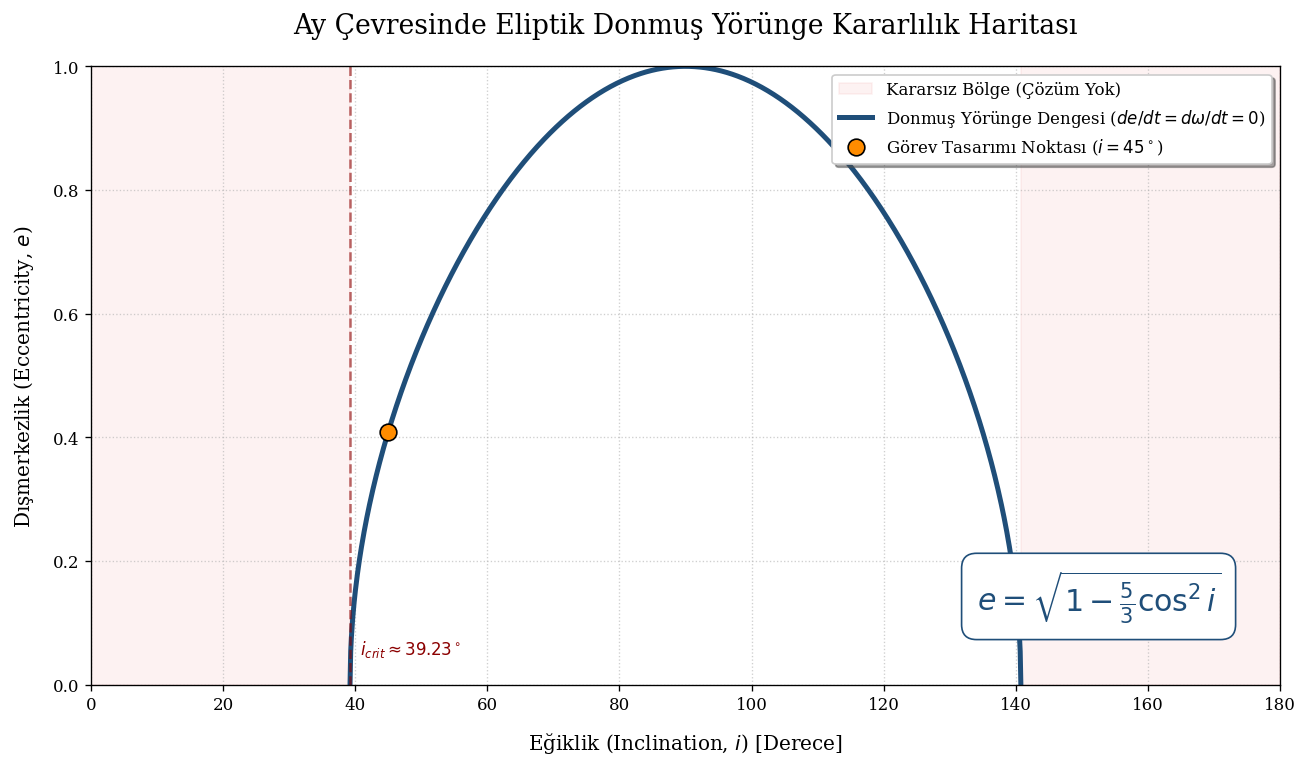
\includegraphics[width=0.92\linewidth]{Resimler/Ay Modeli/Frozen Orbit.png}
    \caption{Ay çevresinde eliptik donmuş yörünge denge eğrisi: $\dot{e}=0$ ve $\dot{\omega}=0$ koşullarını sağlayan
    analitik çözüm ailesi ve kritik eğiklik ($i_{\mathrm{crit}}\approx 39.23^\circ$) bölgesi.}
    \label{fig:frozen_orbit_map}
\end{figure}


Frozen testinin ayırt edici olabilmesi için seçilen yörünge, (i) kısa dalga boylu yerçekimi içeriğini
(har.\ yüksek derece terimleri / mascon etkileri) dinamiğe yeterince yansıtacak kadar ``hassas'',
ancak (ii) topografya kaynaklı çarpışma riski ve integratör hatalarını büyütecek kadar da ``aşırı agresif''
olmayacak şekilde seçilmelidir. Bu dengeyi sağlamak için başlangıç koşulları çoğunlukla aşağıdaki ilkelerle belirlenir:

\begin{itemize}
\item \textbf{Alçak irtifa (yaklaşık 20--60 km perilune yüksekliği):}
yüksek dereceli (kısa dalga boylu) bileşenleri belirginleştirerek mascon kaynaklı yerel anomalilerin
yörünge elemanlarına etkisini görünür kılar. (Bu aralık aynı zamanda topografya nedeniyle emniyet marjı gerektirir.)
\item \textbf{Küçük--orta dışmerkezlik ($e\simeq 0.01$--$0.05$):}
perilune civarında duyarlılığı artırır; buna karşın yüksek $e$ durumlarında görülen ``sertleşme''
(çok farklı zaman ölçekleri / adım-boyu hassasiyeti) etkilerini sınırlı tutarak sayısal kararlılığı korur.
\item \textbf{Polar/polar-yakın eğiklik ($i\approx 90^\circ$):}
geniş kapsama sağlayarak yerel anomalilerin farklı boylamlarda örneklenmesini kolaylaştırır ve
temsil hatalarını ``küresel tarama'' üzerinden ayırt etmeye yardım eder.
\item \textbf{Başlangıç enberi argümanı ($\omega$):}
$\omega=90^\circ$ veya $270^\circ$ seçimleri, analitik donma koşullarında sık çıkan simetrilerle uyumu ve
pratikte bazı konfigürasyonlarda seküler sürüklenmeleri azaltma eğilimi nedeniyle test başlangıcı için kullanışlıdır.
\end{itemize}

\paragraph{Örnek başlangıç parametreleri (temsilî).}
Aşağıdaki örnek, tek bir ``standart'' yörünge önermekten ziyade, testin duyarlılık aralığını
temsil eden tipik bir başlangıç kümesini göstermektedir.

\begin{table}[htbp]
\centering
\caption{Temsilî frozen-test başlangıç yörüngesi (Ay merkezli Kepler elemanları).}
\label{tab:frozen_test_ic}
\small
\begin{tabular}{l c c p{7.2cm}}
\toprule
\textbf{Büyüklük} & \textbf{Sembol} & \textbf{Değer} & \textbf{Not} \\
\midrule
Yarı-büyük eksen & $a$ &
$R_{\text{Moon}} + 40\,\text{km}$ &
Yaklaşık 40 km ortalama irtifa; perilune yüksekliği $h_p=a(1-e)-R_{\text{Moon}}$ ile kontrol edilir. \\
Dışmerkezlik & $e$ & $0.02$ &
Küçük--orta aralık: mascon duyarlılığı $\uparrow$, sayısal sertlik $\downarrow$. \\
Eğiklik & $i$ & $90^\circ$ &
Polar tarama; boylam boyunca örnekleme sağlar. \\
Enberi argümanı & $\omega$ & $90^\circ$ veya $270^\circ$ &
Analitik donma ailesiyle uyumlu başlangıç; bazı durumlarda drift’i bastırabilir. \\
Çıkan düğüm boylamı & $\Omega$ & serbest &
Test senaryosuna bağlı: farklı $\Omega$ seçimi, anomalilerin hangi boylamlarda örneklendiğini değiştirir. \\
Gerçek anomali & $\nu$ & $0^\circ$ &
Başlangıçta perilune’dan başlatma (en yüksek duyarlılık bölgesi). \\
\bottomrule
\end{tabular}
\end{table}

\paragraph{İzlenecek çıktılar ve değerlendirme.}
Frozen testinin amacı, seçilen yörünge elemanlarının uzun dönem davranışının \emph{model içeriğine} (örn.\ derece bandı,
mascon/sferik harmonik temsili, regularization) ne kadar duyarlı olduğunu nicel olarak ortaya koymaktır. Bu amaçla
$e(t)$, perilune yarıçapı $r_p(t)=a(t)\,[1-e(t)]$ (veya perilune yüksekliği $h_p(t)=r_p(t)-R_{\text{Moon}}$),
$\omega(t)$ ve $\Omega(t)$ zaman serileri izlenir. Model karşılaştırmasında ise, aynı başlangıç koşullarından
başlatılan farklı temsiller arasında oluşan durum farkları $\Delta \mathbf r(t)$ ve $\Delta \mathbf v(t)$; mümkünse
ivme farkı $\Delta \mathbf a(t)$ da raporlanarak ayrışmanın yalnızca eleman düzeyinde değil, dinamik düzeyde de
görünür kılınması sağlanır. İyi yakalanmış bir modelde $e$ ve $h_p$ genellikle kısa periyotlu salınımlar gösterirken,
$\omega$ için belirgin bir seküler sürüklenme beklenmez; bu durum pratikte $\omega(t)$ ve $h_p(t)$ üzerine uygulanan
doğrusal uyumdan elde edilen drift hızlarının küçük kalmasıyla test edilebilir. Buna karşılık $\omega$ veya $h_p$’de
monoton bir drift gözlenmesi, yerçekimi temsilinin dinamik açıdan eksik kaldığına (örn.\ yüksek derece içeriğin yetersizliği
veya yerel anomalilerin zayıf temsili) işaret eder. Bir sonraki bölümde bu ölçütler, seçilen entegratör ve gravite temsilleriyle
yürütülen sayısal propagasyonlar üzerinden uygulanacaktır.




% ============ Simülasyon Fazı ==============
\chapter{Sayısal Hesaplama ve Simülasyon}

\section{Giriş}
Bu bölümde, önceki bölümlerde analitik olarak elde edilen yerçekimi modelleri, mascon/SH temsilleri ve donmuş
yörünge koşullarının, sayısal simülasyon ortamına nasıl aktarıldığı açıklanmaktadır. Özellikle Ay çevresinde
yüksek dereceli harmonik içerik ve yerel anomalilerin (mascon etkilerinin) belirgin olması nedeniyle, analitik
yaklaşımların geçerlilik sınırları ve sayısal entegrasyonda ortaya çıkan hata kaynakları (adım-boyu seçimi,
toleranslar, kuvvet modeli tutarlılığı ve başlangıç koşullarının duyarlılığı) kritik hale gelmektedir.
Bu nedenle burada, (i) kullanılan dinamik modelin hangi bileşenlerden oluştuğu, (ii) entegrasyon yönteminin
seçimi ve uygulanışı, (iii) doğrulama/karşılaştırma kriterleri ve (iv) sonuçların fiziksel yorumlanmasında
dikkat edilmesi gereken noktalar sistematik biçimde ele alınacaktır.




% ================== Cowell Yöntemi =================
\newpage
\section{Cowell Yöntemi: Doğrudan Sayısal Entegrasyon}

Yörünge mekaniğinde ``Özel Pertürbasyon'' (\textit{Special Perturbation}) yaklaşımlarının en temel örneklerinden biri
Cowell yöntemidir. Bu yöntemde hareket denklemleri, etkiyen tüm ivmelerin Kartezyen koordinatlardaki vektörel toplamı
üzerinden yazılır ve durum vektörü $\mathbf{x}=[\mathbf{r}\ \mathbf{v}]^{\mathsf T}$ doğrudan sayısal olarak entegre edilir.
Analitik çözümlerin zorlaştığı (yüksek dereceli yerçekimi alanları, yerel anomaliler, çok-cisim pertürbasyonları vb.)
durumlarda kuvvet modelinin ayrıntısı doğrudan dinamiğe yansıtılabildiği için Cowell yöntemi günümüzde yaygın bir
referans yörünge ilerletme yaklaşımıdır. Pratikte yöntem, kuvvet modelini modüler biçimde genişletmeye elverişlidir;
örneğin merkezî çekim yanında yüksek dereceli küresel harmonikler, üçüncü-cisim çekimi ve diğer küçük etkiler aynı çerçevede toplanabilir. Özellikle düşük irtifalarda model ayrıntısı arttıkça, integratör toleransları ve adım-boyu seçimi sonuçların güvenilirliğinde belirleyici hale gelir.


\begin{tcolorbox}[
  colback=gray!10!white,
  colframe=black!75!black,
  title=\textbf{Tarihçe: Halley Kuyruklu Yıldızı ve Cowell'ın Yaklaşımı}
]
Cowell yöntemi adını İngiliz astronom \textbf{Philip Herbert Cowell} (1870--1949)'dan alır. Cowell ve A.\ C.\ D.\ Crommelin,
\textbf{Halley Kuyruklu Yıldızı'nın 1910 geçişini} öngörmek için Jüpiter ve Satürn başta olmak üzere gezegen pertürbasyonlarını
hesaba katarak adım-adım sayısal entegrasyon uygulamış, günberi zamanını yaklaşık \textbf{3 günlük bir farkla} yakalayabilmiştir.
Bu sonuca, dönemin koşullarında \textbf{yaklaşık üç yıl} süren yoğun el hesabı ve tablo çalışmasıyla ulaşılmıştır. Bu çalışma,
``doğrudan entegrasyon'' fikrinin yalnızca teorik bir seçenek olmadığını, yeterli emek ve dikkatli kuvvet modeliyle
yüksek doğruluğa ulaşabildiğini göstermesi bakımından dönüm noktasıdır.

\medskip
Yöntem aslında oldukça yüksek doğruluk vaat etse de, o dönemde hesaplamaların büyük kısmı elle yapıldığı için
\textbf{hesaplama maliyeti} çok yüksekti ve bu da yaygın kullanımını uzun süre sınırladı. Elektronik hesap makineleri ve
modern sayısal integratörler geliştikçe Cowell yaklaşımı yeniden pratik hale geldi ve bugün yörünge propagasyonunda
en sık kullanılan yöntemlerden biri olarak yerini aldı.

\end{tcolorbox}

\subsection{Alternatif Bir Yaklaşım: Encke Yöntemi}

Cowell yöntemi toplam ivmeyi entegre ederken, \textbf{Encke yöntemi} referans bir yörünge (genellikle Kepler yörüngesi)
ile gerçek yörünge arasındaki farkı ($\delta\mathbf{r}$) entegre eder. Temel fikir, ``küçük'' farkların sayısal olarak
daha kararlı ve hataya daha az duyarlı biçimde izlenebilmesidir. Basit gösterimle:
\begin{equation}
\delta \ddot{\mathbf{r}}
= \mathbf{a}_{\text{total}}(\mathbf{r}_{\text{ref}}+\delta\mathbf{r},t) - \mathbf{a}_{\text{ref}}(\mathbf{r}_{\text{ref}},t),
\end{equation}
burada $\mathbf{a}_{\text{ref}}$ referans (Kepler) yörüngesine ait ivmeyi temsil eder. Bu yaklaşımda $\delta\mathbf{r}$
küçük kaldığı sürece, çözümü doğrudan ``tam'' vektörler üzerinde taşımak yerine yörüngeyi referansa göre küçük bir düzeltme
olarak takip etmek, yuvarlama hatalarının birikimini azaltabilir.


\smallskip
Encke yöntemi, bilgisayarların sınırlı olduğu dönemlerde yuvarlama hatalarını azaltma açısından cazipti; ancak referans
yörüngenin periyodik güncellenmesi (\emph{rectification}) gerekliliği ve uygulama karmaşıklığı nedeniyle, modern integratörler ve işlem gücüyle birlikte pratikte çoğu senaryoda Cowell yaklaşımı daha tercih edilir hale gelmiştir.





% ================ Cowell Yönteminin Türetilmesi ==============
\subsection{Cowell Yönteminin Matematiksel Formülasyonu}
\label{subsec:cowell_math}

Cowell yöntemi, Newton hareket yasalarının yörünge problemine en doğrudan uygulanışıdır:
uydunun konumu ve hızı Kartezyen uzayda taşınır ve her entegrasyon adımında, seçilen kuvvet modelinden elde edilen
\textbf{toplam ivme} doğrudan kullanılır. Eylemsiz bir referans çerçevesinde (ör.\ J2000 benzeri) hareket denklemi
genel olarak
\begin{equation}
\label{eq:cowell_basic}
\ddot{\mathbf r}(t)=\mathbf a_{\text{total}}(\mathbf r,\mathbf v,t)
= -\frac{\mu}{r^{3}}\mathbf r \;+\;\mathbf a_{\text{pert}}(\mathbf r,\mathbf v,t)
\end{equation}
şeklinde yazılır. Burada $\mu$ merkezi cismin standart çekim parametresi, $\mathbf r=[x\ y\ z]^{\mathsf T}$ konum vektörü
ve $r=\|\mathbf r\|$ büyüklüğüdür. $\mathbf a_{\text{pert}}$ ise merkezî iki-cisim teriminin dışında kalan tüm bozucu
ivmelerin toplamını temsil eder.

Ay çevresi gibi yüksek dereceli yerçekimi içeriğinin önemli olduğu problemlerde $\mathbf a_{\text{pert}}$ tipik olarak
aşağıdaki bileşenlerden oluşur:
\begin{equation}
\label{eq:apert_components}
\mathbf a_{\text{pert}}
= \mathbf a_{\text{asph}}
+ \mathbf a_{\text{3rd}}
+ \mathbf a_{\text{SRP}}
+ \mathbf a_{\text{tidal}}
+ \dots
\end{equation}
Bu çalışmada dinamiği belirleyen ana bileşen $\mathbf a_{\text{asph}}$ olup, küresel harmonik katsayılarından türetilen
(asferik) yerçekimi ivmesini ve dolaylı olarak mascon kaynaklı kısa dalga boylu anomalileri içerir. Üçüncü-cisim terimi
$\mathbf a_{\text{3rd}}$ genellikle Dünya ve Güneş gibi pertürbatörlerin çekimini; $\mathbf a_{\text{SRP}}$ güneş radyasyon
basıncını temsil eder. Kullanım senaryosuna bağlı olarak gelgit/şekil değişimi gibi ek terimler de modele eklenebilir.

\subsubsection{Birinci Dereceden Denklem Sistemine İndirgeme}
\label{subsubsec:first_order_reduction}

Sayısal entegratörlerin büyük kısmı birinci dereceden sistemler üzerinden çalıştığı için
\eqref{eq:cowell_basic} denklemi durum-uzayı biçimine dönüştürülür. Durum vektörü
\begin{equation}
\mathbf X(t)=
\begin{bmatrix}
\mathbf r(t)\\
\mathbf v(t)
\end{bmatrix}
=
\begin{bmatrix}
x\\y\\z\\\dot x\\\dot y\\\dot z
\end{bmatrix}
\end{equation}
olarak tanımlanırsa, sistemin türevi
\begin{equation}
\label{eq:state_space}
\dot{\mathbf X}(t)=
\begin{bmatrix}
\dot{\mathbf r}(t)\\
\dot{\mathbf v}(t)
\end{bmatrix}
=
\begin{bmatrix}
\mathbf v(t)\\
\mathbf a_{\text{total}}(\mathbf r,\mathbf v,t)
\end{bmatrix}
=
\begin{bmatrix}
\dot x\\ \dot y\\ \dot z\\
-\dfrac{\mu}{r^3}x + a_{\text{pert},x}\\
-\dfrac{\mu}{r^3}y + a_{\text{pert},y}\\
-\dfrac{\mu}{r^3}z + a_{\text{pert},z}
\end{bmatrix}
\end{equation}
şeklini alır. Böylece problem, $\mathbf X(t_0)$ başlangıç koşulundan başlayarak $\dot{\mathbf X}=f(t,\mathbf X)$ formunda
doğrudan propagasyona indirgenmiş olur.


% =============== Referans Dönüşümleri ======================
\section{Referans Çerçevesi Dönüşümleri ve Zaman Ölçekleri}
\label{sec:frame_transforms}

Küresel harmonik yerçekimi katsayıları pratikte \textbf{cisme bağlı} (\emph{body-fixed}) bir çerçevede tanımlanır;
çünkü asferik alan, cismin dönmesiyle birlikte uzayda ``döner''. Buna karşılık Cowell yörünge ilerletimi,
hesap kolaylığı ve dış pertürbasyonların (3.\ cisim, SRP vb.) tutarlı ifadesi nedeniyle çoğunlukla \textbf{eylemsiz}
bir çerçevede yürütülür. Bu yüzden yüksek doğruluk için her ivme değerlendirmesinde (i) konumu body-fixed çerçeveye
taşımak, (ii) ivmeyi bu çerçevede hesaplamak ve (iii) ivmeyi tekrar eylemsiz çerçeveye geri döndürmek gerekir.

% ------------------------------------------------------------
\subsection{Eylemsiz ve Body-Fixed Çerçeveler}
\label{subsec:inertial_bodyfixed}

Yörünge dinamiğinde referans çerçevesi seçimi, hangi eksen takımının ``sabit'' kabul edildiğini belirler.
\textbf{Eylemsiz (inertial) çerçeve} dış torkların ihmal edilebilir olduğu ölçekte Newton yasalarının en sade biçimde
yazılabildiği eksen takımıdır. Uygulamada tam anlamıyla eylemsiz bir çerçeve yoktur; ancak GCRF/J2000 gibi astronomik
referanslara bağlanan çerçeveler, tipik görev sürelerinde eylemsiz kabul edilerek entegrasyon için doğal bir seçim sağlar.

\medskip
\textbf{Body-fixed (cisme bağlı) çerçeve} ise cismin gövdesiyle birlikte dönen eksen takımıdır. Dünya için Earth-fixed
çerçevede topoğrafya ve yerçekimi katsayılarının tanımlı olduğu boylam/enlem sistemi, Dünya ile birlikte döner.
Ay için de Moon-fixed bir çerçeve aynı mantıkla tanımlanır: topoğrafya, mascon yapıları ve küresel harmonik katsayıları
bu dönen çerçevede sabittir. Dolayısıyla küresel harmoniklerden ivme hesaplamak en doğal biçimde body-fixed eksenlerde yapılır.

Bu bölüm boyunca aşağıdai iki çerçeve kullanılacaktır:
\begin{itemize}
\item $\mathcal I$: Eylemsiz çerçeve (örn.\ J2000/GCRF benzeri).
\item $\mathcal B$: Body-fixed çerçeve (Ay için ``Moon-fixed'', Dünya için ``Earth-fixed'' benzeri).
\end{itemize}

% ------------------------------------------------------------
\subsubsection{Yön kosinüs matrisi (DCM) nedir?}
\label{subsubsec:dcm_intro}

İki referans çerçevesi arasında vektör bileşenlerini dönüştürmenin en standart yolu \textbf{yön kosinüs matrisi}
(\emph{Direction Cosine Matrix}, DCM) kullanmaktır. DCM, iki eksen takımının birbirine göre yönelimini kodlayan,
\textbf{$3\times3$} boyutlu saf bir \textbf{dönme} matrisidir.

$\mathcal I$ çerçevesinin birim eksenleri
$\{\hat{\mathbf i}_1,\hat{\mathbf i}_2,\hat{\mathbf i}_3\}$, $\mathcal B$ çerçevesinin birim eksenleri ise
$\{\hat{\mathbf b}_1,\hat{\mathbf b}_2,\hat{\mathbf b}_3\}$ olsun. O zaman
$\mathbf C_{\mathcal B\leftarrow\mathcal I}$ matrisinin elemanları
\begin{equation}
\label{eq:dcm_elements}
\big[\mathbf C_{\mathcal B\leftarrow\mathcal I}\big]_{jk}
=\hat{\mathbf b}_j \cdot \hat{\mathbf i}_k
\end{equation}
şeklinde tanımlanır; yani her eleman iki eksenin yaptığı açının kosinüsüdür.

Bu tanımı açık matris biçiminde de yazabiliriz:
\begin{equation}
\label{eq:dcm_matrix}
\mathbf C_{\mathcal B\leftarrow\mathcal I}=
\begin{bmatrix}
\hat{\mathbf b}_1\!\cdot\!\hat{\mathbf i}_1 & \hat{\mathbf b}_1\!\cdot\!\hat{\mathbf i}_2 & \hat{\mathbf b}_1\!\cdot\!\hat{\mathbf i}_3\\
\hat{\mathbf b}_2\!\cdot\!\hat{\mathbf i}_1 & \hat{\mathbf b}_2\!\cdot\!\hat{\mathbf i}_2 & \hat{\mathbf b}_2\!\cdot\!\hat{\mathbf i}_3\\
\hat{\mathbf b}_3\!\cdot\!\hat{\mathbf i}_1 & \hat{\mathbf b}_3\!\cdot\!\hat{\mathbf i}_2 & \hat{\mathbf b}_3\!\cdot\!\hat{\mathbf i}_3
\end{bmatrix}.
\end{equation}

DCM saf bir dönme olduğu için iki temel özelliğe sahiptir:
\begin{equation}
\label{eq:dcm_orthonormal}
\mathbf C_{\mathcal B\leftarrow\mathcal I}\,\mathbf C_{\mathcal B\leftarrow\mathcal I}^{\mathsf T}
=\mathbf I,
\qquad
\mathbf C_{\mathcal B\leftarrow\mathcal I}^{-1}
=\mathbf C_{\mathcal B\leftarrow\mathcal I}^{\mathsf T}.
\end{equation}
Yani matris ortonormâldir; uzunlukları korur ve ters dönüşüm transpoz ile yapılır.

% ------------------------------------------------------------
\subsubsection{Vektör dönüşümü nasıl okunur?}
\label{subsubsec:vector_transform_read}

Aynı geometrik vektör, farklı çerçevelerde farklı bileşenlerle temsil edilir. Örneğin uzay aracının konumu
$\mathbf r$ olsun; bu vektörün bileşenleri eylemsiz çerçevede $\mathbf r_{\mathcal I}$,
body-fixed çerçevede ise $\mathbf r_{\mathcal B}$ ile gösterilsin. DCM ile dönüşüm
\begin{equation}
\label{eq:ri_to_rb}
\mathbf r_{\mathcal B}(t)=\mathbf C_{\mathcal B\leftarrow\mathcal I}(t)\,\mathbf r_{\mathcal I}(t)
\end{equation}
şeklindedir. Bu ifade, ``eylemsizde bilinen bileşenleri o anki yönelime göre body-fixed eksenlere projekte et'' diye okunur.

İvme gibi bir vektörü body-fixed çerçevede hesapladıktan sonra, Cowell entegrasyonuna geri beslemek için eylemsize dönmek gerekir:
\begin{equation}
\label{eq:ab_to_ai}
\mathbf a_{\mathcal I}(t)=\mathbf C_{\mathcal B\leftarrow\mathcal I}^{\mathsf T}(t)\,\mathbf a_{\mathcal B}(t).
\end{equation}

\subsubsection{Neden bu dönüşüm şart?}
\label{subsubsec:why_transform}

Küresel harmonik katsayıları $\bar C_{\ell,m},\bar S_{\ell,m}$ belirli boylam/enlem yapılarıyla ilişkilidir ve bu yapı
cismin dönmesiyle birlikte uzayda döner. Eğer konumu eylemsiz çerçevede bırakıp bu dönmeyi ``yok sayarsanız'',
özellikle $m\neq0$ (tesseral/sectoral) terimlerin fazı yanlış olur. Bu tür bir faz hatası, alçak irtifada ve
rezonans bölgelerinde zamanla birikerek yapay sürüklenmelere ve konum hatalarına yol açabilir.
Bu yüzden yüksek doğruluk hedefleniyorsa ivme hesabı doğru çerçevede yapılmalı ve sonuç doğru çerçevede entegratöre verilmelidir.

% ------------------------------------------------------------
\subsection{Zaman ölçekleri: aynı $t$ ile her şeyi tutarlı yapmak}
\label{subsec:time_scales}

Çerçeve dönüşümünün doğruluğu yalnızca matrisin biçimine değil, \textbf{zaman argümanının hangi ölçeğe göre tanımlandığına}
da bağlıdır. Pratikte dört zaman ölçeği öne çıkar:
\begin{itemize}
\item \textbf{UTC:} Takvim zamanı (artık saniye içerir). Veri etiketleme ve raporlama için uygundur.
\item \textbf{UT1:} Dünya'nın gerçek dönmesini izler. Dünya için dönme açısı (ERA/GST benzeri) UT1'e bağlıdır.
\item \textbf{TAI/TT:} Düzgün (uniform) zaman ölçekleri. TT, birçok astronomik modelin doğal zaman argümanıdır.
\item \textbf{TDB (ET):} Efemeris zaman ölçeği. Birçok efemeris altyapısı (örn.\ SPICE) dönüşümleri TDB/ET ile verir.
\end{itemize}

Temel kural şudur: entegratörün kullandığı zaman değişkeni ile (i) body orientation (yönelim) fonksiyonları,
(ii) üçüncü-cisim konumları ve (iii) dönme açısı aynı ``mutlak zaman'' tanımıyla beslenmelidir.
Ay uygulamalarında yönelim/librasyon modelleri çoğu zaman TT veya TDB tabanlı verildiği için,
en güvenli yaklaşım dinamik hesabı TT/TDB ekseninde yürütmek ve yalnızca çıktı aşamasında UTC'ye dönmektir.

% ------------------------------------------------------------
\subsection{Dönüşüm matrisi $\mathbf C_{\mathcal B\leftarrow\mathcal I}(t)$ nasıl üretilir?}
\label{subsec:how_to_get_C}

$\mathbf C_{\mathcal B\leftarrow\mathcal I}(t)$, cismin uzaydaki yönelimini temsil eder. Basit modellerde bu yönelim
tek bir dönme açısı ile yaklaşık olarak temsil edilebilir; ancak Ay gibi cisimlerde librasyonlar ve küçük yönelim
varyasyonları nedeniyle yüksek doğruluk için daha tam bir yönelim modeli gerekir.

\subsubsection{Basit model: tek eksen etrafında dönme }
Body-fixed çerçevenin, eylemsiz çerçeveye göre yalnızca $z$ ekseni etrafında $\theta(t)$ kadar döndüğü varsayılırsa
\begin{equation}
\label{eq:R3_theta_simple}
\mathbf C_{\mathcal B\leftarrow\mathcal I}(t)=\mathbf R_3\!\big(\theta(t)\big)=
\begin{bmatrix}
\cos\theta & \sin\theta & 0\\
-\sin\theta & \cos\theta & 0\\
0 & 0 & 1
\end{bmatrix}.
\end{equation}
Bu yaklaşım, faz mantığını göstermek için yararlıdır; ancak Ay librasyonları ve yüksek hassasiyetli faz kontrolü için tek başına yeterli değildir.

\subsubsection{Standart yönelim modeli: IAU biçimi}
Birçok cisim için yönelim, kuzey kutbunun eylemsiz çerçevede doğrultusu (sağ açıklık $\alpha(t)$, dik açıklık $\delta(t)$)
ve asal meridyen açısı $W(t)$ ile verilir. Bu üçlüden DCM yaygın olarak
\begin{equation}
\label{eq:iau_dcm}
\mathbf C_{\mathcal B\leftarrow\mathcal I}(t)
=
\mathbf R_3\!\big(W(t)\big)\,
\mathbf R_1\!\big(90^\circ-\delta(t)\big)\,
\mathbf R_3\!\big(90^\circ+\alpha(t)\big)
\end{equation}
şeklinde kurulur. Burada $\mathbf R_1(\phi)$ $x$ ekseni etrafında dönme matrisidir:
\[
\mathbf R_1(\phi)=
\begin{bmatrix}
1 & 0 & 0\\
0 & \cos\phi & \sin\phi\\
0 & -\sin\phi & \cos\phi
\end{bmatrix}.
\]
Sezgisel olarak önce dönme eksenini hizalarsınız ($\alpha,\delta$), ardından boylam fazını $W(t)$ ile uygularsınız.

\subsubsection{Efemeris/çekirdek altyapısı }
Uygulamada en güvenilir yol, $\alpha(t)$, $\delta(t)$, $W(t)$ fonksiyonlarını veya doğrudan
$\mathbf C_{\mathcal B\leftarrow\mathcal I}(t)$ matrisini bir efemeris altyapısından almaktır.
Ay için librasyonların etkisi nedeniyle bu tercih, faz hatasını belirgin biçimde azaltır.
Kritik nokta şudur: seçilen yönelim verisi hangi zaman ölçeğini istiyorsa, entegrasyon zamanı onunla tutarlı yürütülmelidir.

\newpage
% ------------------------------------------------------------
\subsection{Asferik ivmenin doğru fazda hesaplanması}
\label{subsec:asph_acc_pipeline}

Küresel harmonik ivme, potansiyelin gradyanı olarak \textbf{body-fixed} çerçevede hesaplanır:
\begin{equation}
\label{eq:a_asph_bodyfixed}
\mathbf a_{\text{asph},\mathcal B}(t)= -\nabla_{\mathcal B}\,
U_{\text{SH}}\!\big(\mathbf r_{\mathcal B}(t)\big).
\end{equation}

Burada yapılan işlem, dinamik denklemleri dönen çerçevede yazmak değildir; alanı doğru çerçevede hesaplayıp ivmenin
\emph{bileşenlerini} eylemsiz çerçeveye taşımaktır. Bu nedenle ayrıca Coriolis/merkezkaç terimleri eklenmez;
yalnızca vektör bileşen dönüşümü uygulanır:
\begin{equation}
\label{eq:ab_to_ai_asph}
\mathbf a_{\text{asph},\mathcal I}(t)=
\mathbf C_{\mathcal B\leftarrow\mathcal I}^{\mathsf T}(t)\,
\mathbf a_{\text{asph},\mathcal B}(t).
\end{equation}

Özellikle $m\neq 0$ (tesseral/sectoral) terimler kullanıldığında bu zincir zorunludur; aksi halde cismin dönmesi modele
yanlış fazda girer ve zamanla biriken yapay sürüklenmeler ortaya çıkar. Yalnızca zonal (boylamdan bağımsız) terimlerle
sınırlı bir kesme yapılıyorsa dönüşüm hassasiyeti görece azalır; ancak yüksek dereceli tam modellerde
\eqref{eq:ri_to_rb} ve \eqref{eq:ab_to_ai_asph} akışı temel gerekliliktir.

\paragraph{Önerilen hesap akışı (tek ivme çağrısı).}
Cowell entegratörünün her ivme değerlendirmesinde çerçeve-faz tutarlılığı aşağıdaki adımlarla korunur:
\begin{enumerate}
\item Entegratörden $\mathbf r_{\mathcal I}(t)$ ve zaman $t$ alınır (seçilen zaman ölçeği ile tutarlı).
\item Yönelim modeli/efemeris ile $\mathbf C_{\mathcal B\leftarrow\mathcal I}(t)$ üretilir.
\item Konum body-fixed’e taşınır: $\mathbf r_{\mathcal B}(t)=\mathbf C_{\mathcal B\leftarrow\mathcal I}(t)\,\mathbf r_{\mathcal I}(t)$.
\item $U_{\text{SH}}$ ve gradyanı ile $\mathbf a_{\text{asph},\mathcal B}(t)$ hesaplanır.
\item İvme eylemsize döndürülür: $\mathbf a_{\text{asph},\mathcal I}(t)=\mathbf C_{\mathcal B\leftarrow\mathcal I}^{\mathsf T}(t)\,\mathbf a_{\text{asph},\mathcal B}(t)$.
\item Toplam ivmeye eklenir ve entegratöre verilir (merkezî terim ve diğer pertürbasyonlar eylemsiz çerçevede).
\end{enumerate}


% ------------------------------------------------------------
\section{Bozucu ivmenin uygun forma getirilmesi}
\label{sec:perturbing_accel_frames}

Bu bölümde aynı $\mathbf a_{\text{pert}}$ vektörünün,
(i) Cowell için \textbf{Kartezyen} bileşenlerde,
(ii) Gauss için \textbf{RTN} bileşenlerinde
nasıl üretileceği tek bir akış üzerinden özetlenir.

\subsection{Cowell için: Kartezyen ivme vektörü}
\label{subsec:cowell_cart}

Cowell propagasyonunda \eqref{eq:cowell_basic} içine doğrudan
\[
\mathbf a_{\text{pert}}\equiv \mathbf a_{\text{pert},\mathcal I}
\]
konur. Asferik ivme $\mathbf a_{\text{asph},\mathcal I}$,
\eqref{eq:ri_to_rb}--\eqref{eq:ab_to_ai} zinciriyle elde edilir; üçüncü-cisim ve SRP gibi terimler de aynı eylemsiz çerçevede
hesaplanarak toplam ivmeye eklenir. Böylece integratörün gördüğü dinamik,
\eqref{eq:state_space}’teki $\mathbf a_{\text{total}}$ çağrısı içinde tutarlı biçimde toplanmış olur.

\subsection{Gauss için: RTN birim vektörleri ve projeksiyon}
\label{subsec:rtn_projection}

Gauss denklemleri için $\mathbf a_{\text{pert}}$ vektörünün RTN bileşenleri gerekir.
Anlık durumdan (eylemsiz çerçevede) RTN birim vektörleri
\begin{equation}
\hat{\mathbf R}=\frac{\mathbf r}{r},\qquad
\hat{\mathbf N}=\frac{\mathbf h}{h},\ \ \mathbf h=\mathbf r\times\mathbf v,\qquad
\hat{\mathbf T}=\hat{\mathbf N}\times\hat{\mathbf R}
\label{eq:rtn_basis}
\end{equation}
şeklinde tanımlanır. Buna karşılık
\begin{equation}
a_R=\mathbf a_{\text{pert}}\cdot \hat{\mathbf R},\qquad
a_T=\mathbf a_{\text{pert}}\cdot \hat{\mathbf T},\qquad
a_N=\mathbf a_{\text{pert}}\cdot \hat{\mathbf N}
\label{eq:rtn_components}
\end{equation}
ile Gauss denklemlerine girecek bileşenler elde edilir.
Bu projeksiyonun avantajı, bozucu ivmenin yörünge düzlemi içi/dışı etkilerinin fiziksel olarak daha doğrudan yorumlanabilmesidir.

\subsection{Özet algoritma: SH ivmeden Cowell ve Gauss’a}
\label{subsec:algo_summary}

Aşağıdaki akış, her iki yöntem için ortak bir ``ivme üretim çekirdeği'' tanımlar:
\begin{enumerate}
\item Entegrasyon durumundan $\mathbf r_{\mathcal I},\mathbf v_{\mathcal I}$ al.
\item Dönüşüm matrisiyle $\mathbf r_{\mathcal B}=\mathbf C_{\mathcal B\leftarrow\mathcal I}(t)\mathbf r_{\mathcal I}$ hesapla.
\item $\mathbf a_{\text{asph},\mathcal B}=-\nabla_{\mathcal B}U_{\text{SH}}(\mathbf r_{\mathcal B})$ ile asferik ivmeyi üret.
\item $\mathbf a_{\text{asph},\mathcal I}=\mathbf C_{\mathcal B\leftarrow\mathcal I}^{\mathsf T}(t)\mathbf a_{\text{asph},\mathcal B}$ ile eylemsize döndür.
\item Diğer pertürbasyonları (3.\ cisim, SRP, vb.) eylemsiz çerçevede hesapla ve $\mathbf a_{\text{pert},\mathcal I}$ içinde topla.
\item Cowell: \eqref{eq:state_space} içinde $\mathbf a_{\text{total}}=-\mu r^{-3}\mathbf r + \mathbf a_{\text{pert},\mathcal I}$ kullan.
\item Gauss: \eqref{eq:rtn_basis}--\eqref{eq:rtn_components} ile $(a_R,a_T,a_N)$ üret ve Gauss denklemlerini entegre et.
\end{enumerate}

% ------------ Uygulamada Dikkat Edilmesi Gerekenler ---------
\subsection{Uygulamada Dikkat Edilmesi Gereken Hususlar}
\label{subsec:cowell_practical}

Cowell propagasyonunun güvenilir olması, yalnızca entegratör mertebesine değil, kuvvet modelinin ve sayısal ayarların
birbiriyle tutarlı seçilmesine de bağlıdır. Bu nedenle uygulamada aşağıdaki noktalar özellikle önemlidir:

\begin{enumerate}
\item \textbf{Kartezyen durum ile tekilliklerden kaçınma.}
Cowell yöntemi doğası gereği $\mathbf r$ ve $\mathbf v$ üzerinden çalışır.
Bu tercih, yörünge elemanlarında $e\approx 0$ (dairesel) veya $i\approx 0$ (ekvatoryal) durumlarında ortaya çıkan
tekilliklerden kaçınmayı sağlar. Dolayısıyla aynı propagasyon çekirdeği, çok farklı yörünge geometrileri için
ek özel durum kodu gerektirmeden kullanılabilir.

\item \textbf{Dönüşüm maliyeti ve doğruluk.}
Yüksek dereceli asferik ivme hesabında her adımda \eqref{eq:ri_to_rb}--\eqref{eq:ab_to_ai} dönüşümleri yapılır.
Bu dönüşümlerin doğruluğu, özellikle $m\neq 0$ terimlerin fazını belirlediği için sonuç üzerinde doğrudan etkilidir.
Dolayısıyla ``yaklaşık'' bir dönme açısı kullanmak yerine, seçilen yönelim modelinin/efemerisin simülasyonla tutarlı olması
yüksek doğruluğun ön koşuludur.

\item \textbf{Adım-boyu ve toleranslar.}
Ay gibi yerel anomalilerin belirgin olduğu cisimlerde ivme alanı kısa mesafelerde değişebilir.
Bu nedenle adaptif adımlı integratörlerde (\texttt{DOP853} vb.) \texttt{RelTol}/\texttt{AbsTol} değerleri,
perilune civarındaki hızlı değişimleri yakalayacak kadar sıkı seçilmeli; seçimin sonuçlara etkisi de yakınsama testiyle
(doğruluğu artırılmış ikinci bir koşu ile) kontrol edilmelidir.

\item \textbf{Sayısal hassasiyet ve ölçekleme.}
Merkezî ivme ile asferik/diğer pertürbasyonlar genellikle farklı mertebelerdedir; bu da yuvarlama hatalarının birikimini
hızlandırabilir. Çift hassasiyet (64-bit) çoğu mühendislik uygulaması için yeterli olsa da, çok sıkı toleranslarda veya çok
uzun süreli propagasyonlarda ölçekleme/nondimensionalization ve gerekirse daha yüksek hassasiyetli aritmetik seçenekleri
değerlendirilmelidir.
\end{enumerate}


% =============== İntegratör Seçimleri ===============
\newpage
\section{Sayısal Entegratör Seçimi ve Algoritmalar}

Cowell yöntemi gibi doğrudan ilerletim (propagasyon) formülasyonlarında hareket denklemleri,
çoğu zaman analitik kapalı-form çözümü olmayan, kuvvet modele bağlı \textbf{lineer olmayan} diferansiyel denklemlerdir.
Bu nedenle yörüngeyi zaman içinde elde etmek için sayısal entegrasyon zorunludur. Ancak ``hangi entegratör?''
sorusu yalnızca yöntemin mertebesiyle yanıtlanmaz; seçilen algoritma, hatayı nasıl denetlediğinizi,
hesabı ne kadar pahalıya getirdiğinizi ve uzun vadede fiziksel korunum davranışını doğrudan belirler.
Bu bölümde entegratör seçimini belirleyen temel ölçütler aşağıdaki gibi özetlenebilir:

\begin{itemize}
    \item \textbf{Hata kontrolü ve hassasiyet:} Yerel kesme hatasının (local truncation error) toleranslara göre
    denetlenmesi; $\texttt{rtol}$ ve $\texttt{atol}$ seçiminin doğruluk üzerindeki etkisi.
    \item \textbf{Hesaplama maliyeti:} Bir adımda kaç kez kuvvet/ivme hesabı gerektiği; özellikle küresel harmonik gibi
    pahalı kuvvet modellerinde adım sayısı ve fonksiyon çağrısı sayısının belirleyici olması.
    \item \textbf{Adım-boyu stratejisi:} Sabit adımın (fixed step) verimlilik sınırları ve adaptif adım-boyunun
    (variable/adaptive step) hızlı değişen dinamiklerde (perilune/perigee geçişi gibi) sağladığı avantaj.
    \item \textbf{Uzun dönem kararlılık ve korunum:} Yıllar ölçeğinde enerji/açısal momentum drift’i; korunumlu
    sistemlerde simplektik yöntemlerin avantajı ve Runge--Kutta ailesinde drift riskinin yönetimi.
    \item \textbf{Yöntemin geometrik özellikleri:} Hamiltonyen/faz-uzayı yapısını ne ölçüde koruduğu; özellikle
    ``niteliksel doğruluk'' (qualitative fidelity) gerektiren uzun süreli analizlerde önem kazanması.
\end{itemize}


\subsection{Geleneksel (Sabit Adımlı) Yöntemler}
Sabit adımlı (fixed step-size) klasik entegratörler, modern \emph{hassas} astrodinamikte çoğu zaman birincil tercih değildir.
Bunun temel nedeni, yörünge dinamiğinin her noktada aynı “zorlukta” olmamasıdır: araç periapsis (perigee/perilune) civarında
hızlı hareket eder ve ivme vektörü daha hızlı değişir; apoapsis civarında ise değişimler daha yavaştır.
Sabit adımlı bir yöntem, periapsis bölgesini yakalayacak kadar küçük bir adım seçildiğinde apoapsiste gereksiz hesap yükü doğurur;
apoapsise göre seçildiğinde ise periapsiste hata büyür ve faz/enerji sapması hızla birikebilir.

Buna rağmen bu yöntemler iki açıdan önemlidir: (i) hata mertebelerini ve sayısal drift mekanizmasını sezgisel biçimde öğretir,
(ii) daha gelişmiş adaptif veya geometrik entegratörlerle kıyaslama yapılırken “taban çizgisi” (baseline) sağlar.
Aşağıdaki yöntemler, Taylor açılımından türetilen klasik şemaların temsilî örnekleridir.

\begin{itemize}
    \item \textbf{Euler Yöntemi (1.\ mertebe):}
    En basit açık (explicit) yöntemdir. Taylor açılımında yalnızca birinci türev terimini tutar ve türevi adım boyunca sabit kabul eder.
    Küresel (global) hata mertebesi $\mathcal{O}(h)$ olduğundan, hata her adımda hızlı birikme eğilimindedir.
    Özellikle yörünge gibi korunumlu (conservative) sistemlerde enerji ve açısal momentumda belirgin \emph{seküler drift} üretir;
    pratikte yörüngeyi yapay biçimde “şişirme” veya “sönümleme” davranışı gösterebilir. Bu nedenle hassas yörünge ilerletiminde
    (propagasyonda) genellikle yalnızca örnek olarak kullanılır.

    \item \textbf{Klasik Runge--Kutta 4 (RK4, 4.\ mertebe):}
    Mühendislik uygulamalarında en yaygın sabit adımlı yüksek mertebe yöntemlerden biridir. Her adımda türevi dört farklı noktada
    değerlendirerek dördüncü mertebeden bir yaklaşım üretir; küresel hata mertebesi yaklaşık $\mathcal{O}(h^{4})$’tür.
    Uygun bir adım seçimiyle kısa--orta süreli propagasyonlarda güvenilir sonuçlar verebilir ve Euler’e göre çok daha kararlıdır.
    Ancak RK4, \textbf{adaptif hata kontrolü} içermez: dinamiğin hızlandığı bölgelerde (periapsis) hatayı sınırlamak için
    adımı küçültmek gerekirken, aynı küçük adım apoapsis civarında gereksiz maliyet doğurur.
    Ayrıca RK4 \textbf{simplektik değildir}; bu yüzden uzun süreli integrasyonlarda (özellikle yalnızca konservatif kuvvetler varken)
    enerji drift’i oluşabilir. Bu drift her zaman büyük olmayabilir, fakat “yıllar ölçeğinde kararlılık” gibi hedeflerde
    yöntem seçimini doğrudan etkiler.
\end{itemize}

\noindent
Özetle, sabit adımlı klasik yöntemler güçlü bir kavramsal temel ve hızlı bir karşılaştırma aracı sunar; ancak yüksek dereceli
gravite modelleri, düşük irtifa geçişleri veya uzun süreli kararlılık analizlerinde genellikle adaptif adımlı ve/veya
geometrik (simplektik) yöntemler daha uygun hale gelir.

% ---------------- Değişken Adımlı Yöntemler ---------
\subsection{Değişken Adımlı (Adaptif) Yöntemler ve RK45 Sınıfı}
Astrodinamik problemlerinde sabit adım kullanımı çoğu zaman verimsizdir; çünkü yörünge boyunca dinamiğin “zaman ölçeği”
sabit kalmaz. Örneğin dışmerkezliği yüksek bir yörüngede uzay aracı perilune/perigee civarında çok hızlı hareket eder,
ivme yönü ve büyüklüğü kısa zaman aralıklarında belirgin biçimde değişir; burada küçük adımlar gerekir. Buna karşılık
aposelene/apogee civarında hareket yavaşlar ve ivme daha “yumuşak” değişir; aynı küçük adımı sürdürmek, aynı doğruluk
hedefi için gereksiz hesap yükü doğurur. Adaptif yöntemler bu farkı otomatik yöneterek, “zor” bölgelerde sık örnekleyip
“kolay” bölgelerde adımı büyütür.

Pratikte \textbf{RK45} ifadesi, gömülü iki çözüm üreten adaptif Runge--Kutta çiftlerinin genel adıdır
(yaygın örnekler: Fehlberg 4(5) veya Dormand--Prince 5(4)). Bu yöntemler, her adımda hem çözümü hem de hatayı birlikte
üretir; dolayısıyla adım boyu seçimi kullanıcının elle ayarladığı bir parametre olmaktan çıkar ve toleranslarla kontrol edilir.
Temel mekanizma şöyledir:
\begin{enumerate}
    \item Her adımda iki farklı mertebeden (örn.\ 4.\ ve 5.\ mertebe) çözüm hesaplanır.
    \item İki çözüm arasındaki fark, yerel hata kestirimi (\emph{local error estimate}) olarak kullanılır.
    \item Kestirilen hata, kullanıcının \textbf{bağıl} (\texttt{RelTol}) ve \textbf{mutlak} (\texttt{AbsTol}) toleranslarına göre
    bileşen bazında ölçeklenerek tek bir kabul/red ölçütüne dönüştürülür.
    \item Hata büyükse adım küçültülür ve aynı zaman aralığı yeniden denenir; hata yeterince küçükse adım kabul edilir ve
    bir sonraki adım için $h$ büyütülerek verim artırılır.
\end{enumerate}

\noindent
Bu sınıf yöntemlerin iki pratik avantajı vardır. Birincisi, kullanıcı doğrudan “istenen hata düzeyi”ni (toleransları) tanımlar;
yöntem, adımı buna göre kendisi ayarlar. İkincisi, çıktılar genellikle \emph{zamanda uniform} değildir: entegratör,
ihtiyaç duyduğu anlarda daha sık örnek ürettiğinden, özellikle periapsis geçişlerini yakalamada verimli olur.
Bununla birlikte tolerans seçimi, yalnızca “daha küçük daha iyi” şeklinde düşünülmemelidir: çok sıkı toleranslar,
özellikle kuvvet modeli pahalıysa (yüksek dereceli SH, üçüncü-cisim, SRP vb.), hesap süresini dramatik artırabilir.
Bu nedenle RK45 pratikte çoğunlukla \emph{orta hassasiyetli} görev analizi, hızlı prototipleme ve model karşılaştırma
çalışmalarında “az ayarla güvenilir sonuç” veren bir varsayılan seçenek olarak öne çıkar.

\noindent
Son olarak, değişken adımlı yöntemlerin doğal bir yan ürünü olarak “adım reddi” (step rejection) ve buna bağlı
hesap yükü artışı görülebilir. Bu durum genellikle dinamiğin keskinleştiği bölgelerde ortaya çıkar ve doğru ayarlanmış
toleranslarla yönetilebilir; gerekiyorsa maksimum/minimum adım sınırları ile de pratik kontrol sağlanır.


% ------------ Yüksek Hassasiyet --------------
\subsection{Yüksek Hassasiyet: \texorpdfstring{DOP853}{DOP853} (Dormand--Prince, 8.\ Mertebe)}
Hassasiyet gereksinimi çok yükseldiğinde (örn.\ $10^{-12}$ ve daha sıkı toleranslar, uzun süreli alçak irtifa yörünge
ilerletimi veya yüksek dereceli gravite modelleri), 4--5.\ mertebe adaptif yöntemler hedef doğruluğa ulaşmak için
adımı aşırı küçültme eğilimindedir. Bunun sonucu olarak hem adım sayısı büyür hem de her adımda pahalı olan kuvvet modeli
(özellikle tam küresel harmonik ivme) daha fazla çağrılır. Bu tür senaryolarda \textbf{DOP853} gibi \textbf{yüksek mertebeli}
açık Runge--Kutta yöntemleri pratikte daha verimli hâle gelebilir.

\textbf{DOP853} (Dormand--Prince 8(5,3)), adından da anlaşılacağı gibi yüksek mertebeli bir çözüm üretirken
aynı adım içinde daha düşük mertebeden \emph{gömülü} çözümlerle hata kestirimi de yapar. Böylece yöntem,
\emph{“her adımda yüksek mertebe çöz, hatayı aynı adımda tahmin et, adım boyunu otomatik ayarla”} akışıyla çalışır.
DOP853'ün burada kritik avantajı şudur: aynı tolerans hedefi için, yüksek mertebe sayesinde genellikle
\textbf{daha büyük adımlarla} ilerleyebilir; dolayısıyla toplamda \textbf{daha az adım} ve \textbf{daha az kuvvet çağrısı}
ile benzer (veya daha iyi) doğruluk elde edilebilir.

\paragraph{Neden özellikle Ay alçak irtifada iş görür?}
Ay yerçekimi alanında mascon kaynaklı yerel anomaliler, ivme alanında kısa dalga boylu ve yer yer keskin değişimler üretir.
Alçak irtifada bu değişimler “hızlı dinamik” bölgeler oluşturarak adaptif entegratörün adımı küçültmesine neden olur.
DOP853, hata kontrolünü sıkı tutarken bile yüksek mertebe avantajıyla bu bölgelerde gerekli çözünürlüğü daha verimli sağlayabilir.
Burada altını çizmek gereken nokta şudur: DOP853 “mucize” değildir; başarısı büyük ölçüde
(i) tolerans seçimi, (ii) minimum/maksimum adım sınırları, (iii) kuvvet modelinin sayısal kararlılığı ve
(iv) çerçeve--zaman tutarlılığı (body-fixed$\leftrightarrow$inertial dönüşümleri) gibi ayrıntılara bağlıdır.

\paragraph{Toleransların pratik yorumu (RelTol/AbsTol).}
DOP853'te adım kabul/red kararı, hata vektörünün \texttt{AbsTol} ve \texttt{RelTol} ile ölçeklenmiş normu üzerinden verilir.
Bu, “konum bileşenlerinde metre düzeyi, hız bileşenlerinde m/s düzeyi” gibi farklı büyüklükteki durum değişkenlerinin
tek bir hata ölçütünde dengeli değerlendirilmesini sağlar. Bu yüzden yüksek hassasiyet koşularında yalnızca
\texttt{RelTol} küçültmek yerine, \texttt{AbsTol}'ün de durum vektörünün ölçeğine uygun seçilmesi gerekir
(aksi hâlde bir bileşen grubu gereksiz yere adımı domine edebilir).

\paragraph{Adım-boyu kontrolü ve reddedilen adımlar.}
Yüksek dereceli gravite alanında, bazı zaman aralıklarında hata kestirimi hızla büyüyebilir ve entegratör adımı reddedip
aynı aralığı daha küçük $h$ ile tekrar deneyebilir. Bu davranış normaldir ve adaptif kontrolün bir parçasıdır;
ancak \emph{çok sık} görülüyorsa genellikle şu sorunlara işaret eder:
\begin{itemize}
    \item Toleransların gereğinden sıkı seçilmesi,
    \item Kuvvet modelinde sayısal gürültü (ör.\ Legendre/SH hesabında kararsızlık, normalizasyon uyumsuzluğu),
    \item Çerçeve dönüşümü veya zaman ölçeğinde faz hatası (özellikle $m\neq0$ terimlerde),
    \item Çok büyük maksimum adım sınırı veya zayıf başlangıç adımı seçimi.
\end{itemize}
Bu nedenle DOP853 ile birlikte pratikte \textbf{maksimum adım}, \textbf{minimum adım} ve gerekirse
\textbf{olay (event) tabanlı} kontrol (örn.\ perilune geçişlerinde daha sık örnekleme) gibi sınırlamalar kullanmak,
hem kararlılığı hem de tekrarlanabilirliği artırır.

\paragraph{Ne zaman DOP853 tercih edilmelidir?}
Özetle DOP853, aşağıdaki koşullarda güçlü bir adaydır:
\begin{itemize}
    \item \textbf{Kuvvet modeli pahalı ve hassasiyet yüksekse:} tam SH, çoklu pertürbasyonlar, hassas çerçeve dönüşümleri.
    \item \textbf{Alçak irtifada hızlı değişen ivme alanı varsa:} mascon geçişleri, kısa dalga boylu yerel anomaliler.
    \item \textbf{Uzun süreli analizde faz hatası birikimi kritikse:} küçük ivme farklarının zamanla konum hatasına büyümesi.
\end{itemize}
Buna karşılık \emph{çok uzun dönemli konservatif} problemlerde (enerji davranışı kritikse) simplektik yöntemler daha uygun
olabilir; DOP853 ise çoğu “yüksek doğruluklu görev analizi” koşusunda, adaptif kontrol + yüksek mertebe verimliliğiyle
güçlü bir referans entegratör olarak öne çıkar.


% --------------- Simplektik İntegratörler ------------
\subsection{Uzun Süreli Kararlılık: Simplektik (Symplectic) Entegratörler}

Runge--Kutta ailesi yöntemler, yerel hatayı (\emph{local truncation error}) etkin biçimde kontrol etseler bile
çok uzun zaman ölçeklerinde (binlerce--milyonlarca adım) enerji ve açısal momentum gibi korunum büyüklüklerinde
seküler drift üretme eğilimindedir. Bunun temel nedeni, standart RK yöntemlerinin Hamiltonyen dinamiğin geometrik
yapısını (simplektik iki-formu ve faz uzayı hacmini) genel olarak korumamasıdır. Özellikle korunumlu bir problemde
(baskın biçimde yerçekimi) küçük fakat sistematik sayısal hatalar, uzun vadede ``yapay sönüm'' veya ``yapay enerji artışı''
gibi fiziksel olmayan birikimli etkiler doğurabilir.

\textbf{Simplektik integratörler}, Hamiltonyen sistemlerin bu geometrik yapısını koruyacak şekilde tasarlanır.
Hamiltonyen formda
\[
\dot{\mathbf{q}}=\frac{\partial H}{\partial \mathbf{p}},\qquad
\dot{\mathbf{p}}=-\frac{\partial H}{\partial \mathbf{q}}
\]
ile tanımlanan bir sistemde, simplektik integratörün ayırt edici özelliği, adım adım uygulanan sayısal dönüşümün
(\emph{map}) simplektik olmasıdır; yani faz uzayında hacim korunur (Liouville teoremi ile tutarlı) ve sistemin
kanonik yapısı bozulmaz. Bu nedenle simplektik yöntemler, hatayı her adımda ``en küçük'' yapmaya çalışmak yerine,
hatanın \emph{sınırlı bir bant içinde salınmasını} hedefler. Pratik sonuç şudur: enerji tam olarak sabit kalmasa da,
uzun süreli propagasyonda enerji hatası genellikle \emph{seküler olarak büyümek yerine} sınırlı bir aralıkta dalgalanır.

Astrodinamikte yaygın bir örnek \textbf{Velocity Verlet} (veya ``leapfrog'') şemasıdır. Merkezî çekim gibi
potansiyel--kinetik ayrışması yapılabilen sistemlerde
$H(\mathbf{q},\mathbf{p})=T(\mathbf{p})+V(\mathbf{q})$ yazılabildiğinde,
simplektik yöntemler çoğunlukla ``\textit{drift--kick--drift}'' veya ``\textit{kick--drift--kick}'' biçiminde
uygulanır: önce konumlar yarım adım güncellenir, sonra ivmeye bağlı hız güncellemesi yapılır, ardından konumlar
tamamlanır. Daha yüksek mertebeli simplektik şemalar (\textbf{Yoshida} gibi) ise bu temel adımı belirli katsayılarla
ardışık kompozisyonlar halinde birleştirerek mertebeyi artırır ve yine simplektik yapıyı korur.

\medskip
\noindent\textbf{Ne zaman avantajlı?}
Simplektik entegratörler özellikle \emph{uzun dönemli} (yıllar--yüzyıllar) ve \emph{korunumlu} (konservatif)
problemlerde (Güneş Sistemi dinamiği, uzun süreli yörünge kararlılığı, rezonans analizi vb.) öne çıkar.

\medskip
\noindent\textbf{Sınırları:}
Basınç/sürüklenme, itki, empirik kuvvetler veya sık manevra gibi \emph{korunumlu olmayan} etkiler baskınsa,
``enerji koruma'' hedefi zaten fiziksel olarak geçerli değildir; bu durumda simplektik avantaj azalır ve adaptif adım-boylu,
hata kontrollü RK türleri daha pratik olabilir. Ayrıca klasik simplektik yöntemler çoğunlukla sabit adımlıdır; dinamiğin
çok sertleştiği bölgelerde (örn.\ çok alçak perilune) adım seçimi yine kritik hale gelir.

% ------------------ Nyquist Critical Frequency --------------
\newpage
\subsection{Adım-boyu ve Nyquist Ölçütü}
\label{subsec:nyquist_stepsize}

Yüksek dereceli bir gravite modeli, uzaysal olarak daha kısa dalga boylu (yani daha “ince ölçekli”) bileşenler içerir.
Bir \(N\times N\) küresel harmonik kesmesinde en yüksek derecenin temsil ettiği tipik uzaysal ölçek,
yaklaşık olarak
\begin{equation}
\lambda_N \;\approx\; \frac{2\pi R}{N}
\end{equation}
ile ifade edilebilir (\(R\): cismin yarıçapı). Uzay aracı body-fixed çerçevede yüzey üzerinde yaklaşık
\(v_{\text{rel}}\) göreli hızıyla ilerliyorsa, bu uzaysal dalga boyu zamansal bir ölçeğe dönüşür:
\begin{equation}
T_{\lambda}\;\approx\;\frac{\lambda_N}{v_{\text{rel}}}.
\end{equation}

\textbf{Nyquist mantığı} şunu söyler: bir dalga bileşeninin “yanlış frekansa katlanmaması” (aliasing) için periyot başına
en az iki örnek gerekir. Bu, adım-boyu için en kaba sınırı
\begin{equation}
\Delta t_{\text{Nyq}} \;\lesssim\; \frac{\lambda_N}{2\,v_{\text{rel}}}
\;=\; \frac{\pi R}{N\,v_{\text{rel}}}
\end{equation}
şeklinde verir. Ancak yörünge propagasyonu yalnızca bir sinyali “örnekleme” problemi değildir; entegratör aynı zamanda
dinamiği \emph{integral} olarak biriktirir. Bu nedenle pratikte hedef, Nyquist sınırında “zar zor yakalamak” değil,
kısa dalga boyunu \textbf{yeterli çözünürlükle izlemek} olmalıdır. Mühendislikte yaygın yaklaşım, dalga boyu başına
\(M\) örnek almaktır:
\begin{equation}
\Delta t \;\lesssim\; \frac{\lambda_N}{M\,v_{\text{rel}}},
\qquad
(M \approx 10\text{--}20 \;\;\text{tipik}).
\end{equation}

Burada
\begin{equation}
v_{\text{rel}}\approx \|\mathbf v_{\mathcal I}-\boldsymbol{\omega}\times\mathbf r\|
\end{equation}
yaklaşımı, body-fixed çerçevede “zemin üzerinden akış” hızını kabaca temsil eder. Ay’da \(\|\boldsymbol{\omega}\times\mathbf r\|\)
küçük olduğundan alçak irtifada çoğu durumda \(v_{\text{rel}}\simeq \|\mathbf v\|\) kabulü iyi çalışır; Dünya’da ise UT1’e bağlı
dönme hızı ve enlem etkileri daha belirgin olabilir.

\paragraph{Neden kritik?}
Yanlış adım-boyu yüksek dereceyi boşa çıkarabilir. Eğer \(\Delta t\) büyük seçilirse, modelin en değerli kısmı olan
kısa dalga boylu bileşenler yeterince örneklenemez; bu durumda
(i) yüksek dereceli terimler \emph{yanlış fazda} temsil edilebilir (aliasing),
(ii) ivme alanındaki keskin değişimler “yumuşatılmış” gibi görünür,
(iii) sonuçta yörüngede yapay drift veya beklenmedik rezonans benzeri davranışlar ortaya çıkabilir.
Bu açıdan bakıldığında, aşırı büyük adım-boyu kullanmak \(N\)’yi artırarak elde edilmek istenen kazanımı fiilen “heba eder”.
Dolayısıyla adaptif entegratör kullanılsa bile, \textbf{\texttt{max\_step}} için Nyquist tabanlı bir üst sınır belirlemek
yüksek dereceli propagasyonda koruyucu bir önlemdir.

\paragraph{Sayısal örnek (Ay, dairesel \(h=40\,\mathrm{km}\)).}
Fikir vermesi için \(R_{\text{Moon}}=1737.4\,\mathrm{km}\) ve \(h=40\,\mathrm{km}\) dairesel yörüngede
\(v_{\text{rel}}\approx 1.66\,\mathrm{km/s}\) alınarak, farklı \(N\) değerleri için karakteristik ölçekler ve
adım-boyu sınırları Tablo~\ref{tab:nyquist_moon_steps}’te verilmiştir.
Tablodaki \(\Delta t_{20}\) sütunu, adaptif yöntemlerde \texttt{max\_step} için iyi bir başlangıç rehberi olarak okunabilir.

\begin{table}[h]
\centering
\small
\renewcommand{\arraystretch}{1.15}
\begin{tabular}{c c c c c}
\hline
\textbf{Derece \(N\)} &
\(\boldsymbol{\lambda_N}\) \textbf{(km)} &
\(\boldsymbol{T_{\lambda}}\) \textbf{(s)} &
\(\boldsymbol{\Delta t_{\text{Nyq}}}\) \textbf{(s)} &
\(\boldsymbol{\Delta t_{20}}\) \textbf{(s)} \\ \hline
10  & 1091.6 & 657.1 & 328.6 & 32.9 \\
20  & 545.8  & 328.6 & 164.3 & 16.4 \\
50  & 218.3  & 131.4 & 65.7  & 6.6 \\
120 & 91.0   & 54.8  & 27.4  & 2.7 \\
150 & 72.8   & 43.8  & 21.9  & 2.2 \\
180 & 60.6   & 36.5  & 18.3  & 1.8 \\
\hline
\end{tabular}
\caption{Ay için örnek adım-boyu ölçekleri (dairesel \(h=40\,\mathrm{km}\), \(v_{\text{rel}}\approx 1.66\,\mathrm{km/s}\)).
\(\Delta t_{\text{Nyq}}\): Nyquist alt sınırı (\(M=2\)). \(\Delta t_{20}\): dalga boyu başına 20 örnek (\(M=20\)) önerisi.
Görev hassasiyetine göre \(M=10\text{--}20\) aralığı pratik bir başlangıçtır.}
\label{tab:nyquist_moon_steps}
\end{table}


% ------------ Senaryoya Göre İntegratör Önerisi -----------
\newpage
\subsection{Senaryoya Göre Entegratör Seçimi}
Aşağıdaki tablo, tipik senaryolar için pratik bir başlangıç rehberidir; kesin bir kural olarak değil,
\emph{ilk seçim + doğrulama testi} (yakınsama/tolerans taraması) çerçevesinde okunmalıdır.

\begin{table}[h]
\centering
\small
\renewcommand{\arraystretch}{1.15}
\begin{tabular}{|p{4cm}|p{4cm}|p{6cm}|}
\hline
\textbf{Görev senaryosu} & \textbf{Önerilen entegratör} & \textbf{Gerekçe} \\ \hline

\textbf{LEO (kısa süreli):} \newline Günler--haftalar; basit \(J_2\) ve sınırlı pertürbasyonlar. &
\textbf{RK45 (adaptif)} \newline (hızlı prototipte RK4) &
Adaptif adım, dinamik değişimleri verimli izler. RK4 daha çok hızlı deneme/karşılaştırma içindir. \\ \hline

\textbf{Ay/gezegen (yüksek dereceli gravite):} \newline Örn.\ \(N\ge 100\), alçak irtifa uçuş. &
\textbf{DOP853} \newline (8.\ mertebe, adaptif) &
Yüksek mertebe, aynı hedef tolerans için adım sayısını azaltabilir; mascon geçişlerinde yerel hata daha sıkı tutulur.
Nyquist tabanlı \texttt{max\_step} ile kısa dalga boyu “kaçırılmaz”. \\ \hline

\textbf{Yüksek dışmerkezlik:} \newline Molniya, GTO, kuyruklu yıldız benzeri. &
\textbf{Adaptif adımlı RK} &
Perilune/perigee civarında adım küçülür, apogee civarında büyür; verim sağlar ve yerel hatayı sınırlar. \\ \hline

\textbf{Uzun dönem (korunumlu):} \newline Yıllar--yüzyıllar; konservatif kuvvet modeli. &
\textbf{Simplektik} \newline (Verlet, Yoshida vb.) &
Geometrik yapıyı koruyarak enerji/açısal momentum drift’ini sınırlı tutar; uzun dönem kararlılık analizi için uygundur. \\ \hline

\end{tabular}
\caption{Astrodinamik senaryoları için entegratör seçim rehberi (özet).}
\label{tab:integrator_selection}
\end{table}

Bu çalışma kapsamında, Ay’ın karmaşık kütle çekim alanı (yüksek dereceli küresel harmonikler) ve yüzeye yakın uçuş dinamiği
nedeniyle, yüksek mertebeli ve adaptif adımlı \textbf{DOP853} yöntemi tercih edilmiştir. Uygulamada seçilen
\texttt{RelTol}/\texttt{AbsTol} değerlerinin ve \texttt{max\_step} kısıtının sonuçlara etkisi, aynı senaryonun daha sıkı toleranslar
ve daha küçük \texttt{max\_step} ile tekrarlanması (yakınsama testi) üzerinden doğrulanmalıdır.



% ================== Doğrulama Adımı ==================
\newpage
\section{Model Doğrulama ve Tutarlılık Analizleri}

Geliştirilen bir yörünge simülasyonunun güvenilirliği, yalnızca kodun çalışıyor olmasına değil, üretilen sonuçların
(i) fiziksel yasalarla tutarlı olmasına, (ii) kullanılan kuvvet modellerinin doğru uygulanmasına ve (iii) sayısal
entegrasyonun hedef doğrulukta yakınsak davranmasına bağlıdır. Bu nedenle doğrulama (\textit{verification/validation})
adımı, propagasyon sonuçlarının ``model içeriği'' mi yoksa ``sayısal ayarlar'' mı tarafından belirlendiğini ayırt etmek için
zorunludur. Bu bölümde doğrulama iki seviyede ele alınır: (a) yörüngeye çıkmadan önce alan seviyesinde
(\textit{statik}) kontrol ve (b) aynı başlangıç koşullarında propagasyon yaparak görev seviyesinde (\textit{dinamik}) kontrol.
Amaç, kuvvet modeli, çerçeve dönüşümleri, normalizasyon ve integratör toleranslarının birbirleriyle uyumlu çalıştığını
kanıtlamaktır.

\subsection{Alan Düzeyi Karşılaştırma: Potansiyel ve İvme Farkları}
Yörünge propagasyonuna başlamadan önce, seçilen gravite modelinin ürettiği ivmenin \emph{alan düzeyinde} tutarlı olup olmadığını
kontrol etmek gerekir. Bu adımın nedeni şudur: Eylemsiz--body-fixed dönüşümündeki faz hatası, katsayı normalizasyonu hatası,
derece/sıra kesmesi veya yanlış referans yarıçapı/GM kullanımı, yörüngeye geçmeden önce bile ``ivme alanında'' kendini belli eder.
Dolayısıyla önce ivmenin kendisi doğrulanır; böylece dinamik testlerde görülen farkların kaynağı daha net ayrıştırılır.

Bu amaçla aynı irtifa küresi üzerinde iki model karşılaştırılır (ör.\ $120\times120$ ile $50\times50$ veya bir ``referans'' SH
modeli ile). İvme farkı
\begin{equation}
\Delta \mathbf{a}(\mathbf{r}) = \mathbf{a}_{\text{Model}}(\mathbf{r}) - \mathbf{a}_{\text{Ref}}(\mathbf{r})
\end{equation}
şeklinde tanımlanır. Uygulamada bu işlem şu şekilde yapılır:
(i) seçilen irtifa için bir küre üzerinde $S$ adet nokta örneklenir (ör.\ enlem-boylam grid'i veya Fibonacci küre örneklemesi),
(ii) her noktada iki modelden $\mathbf a(\mathbf r_k)$ hesaplanır, (iii) fark normu
$||\Delta \mathbf a(\mathbf r_k)||$ haritalanır ve özet istatistikler çıkarılır.

Küresel ölçekte tek bir sayı ile kıyaslamak için RMS metriği kullanılır:
\begin{equation}
RMS_{\Delta a}=\sqrt{\frac{1}{S}\sum_{k=1}^{S}\left\|\Delta\mathbf a(\mathbf r_k)\right\|^{2}}.
\end{equation}
RMS, genel büyüklüğü verir; ancak tek başına yeterli değildir. Bu nedenle raporlama sırasında
\emph{maksimum} değer ($\max_k ||\Delta\mathbf a||$) ve mümkünse bileşen bazında (radial/tangential/normal) farklar da
incelenmelidir. Eğer yüksek dereceli model, fiziksel olmayan ``spike'' benzeri sivri uçlar veya lokal patlamalar gösteriyorsa,
bu durum çoğunlukla (a) aşırı yüksek derece bandında gürültü/overfitting, (b) yanlış normalizasyon, (c) sayısal instabilite
veya (d) dönüşüm fazı hatası gibi kök nedenlere işaret eder. Böyle bir anomali dinamik teste geçmeden önce giderilmelidir.

\newpage
\subsection{Görev Düzeyi Karşılaştırma: Farkların Birikimi (Dinamik Doğrulama)}
Alan düzeyindeki küçük farklar, propagasyon sırasında entegre edilerek konum/hız farklarına dönüşür.
Bu nedenle ikinci adım, aynı başlangıç koşullarından başlatılan iki koşunun zaman içinde nasıl ayrıştığını ölçmektir.
Bu testin amacı, beklenen davranışın \emph{model kaynaklı} mı yoksa \emph{sayısal hata kaynaklı} mı olduğunu anlamaktır.

İki farklı model (ör.\ $50\times50$ ve $120\times120$) aynı $\mathbf r(t_0),\mathbf v(t_0)$ ile başlatıldığında,
konum sapması
\begin{equation}
\left\|\Delta \mathbf{r}(t)\right\|
= \left\|\mathbf{r}_{120}(t)-\mathbf{r}_{50}(t)\right\|
\end{equation}
olarak izlenir (benzer şekilde $\|\Delta\mathbf v(t)\|$). Pratikte bu test şu şekilde yürütülür:
\begin{enumerate}
\item Aynı integratör ve aynı toleranslarla iki koşu yapılır (yalnızca gravite modeli farklı).
\item $\|\Delta\mathbf r(t)\|$ ve $\|\Delta\mathbf v(t)\|$ zaman serileri kaydedilir.
\item Ayrışmanın karakteri değerlendirilir: periyodik mi, yavaş seküler mi, yoksa yüksek frekanslı ``tırtıklı'' bir gürültü mü?
\end{enumerate}
Beklenti, model farklarının genellikle belirli bir ölçüde \emph{düzenli} (seküler veya periyodik) bir ayrışma üretmesidir.
Buna karşılık ayrışma sinyali tamamen rastgele ve adım-boyuna aşırı hassassa, asıl baskın etkenin sayısal hata
(\textit{numerical noise}) olması mümkündür. Bu ayrımı yapmak için en kritik kontrol,
\textbf{yakınsama testi}dir: aynı senaryo daha sıkı toleranslarla yeniden çalıştırılır ve $\|\Delta\mathbf r(t)\|$ eğrisinin
şekli anlamlı biçimde değişiyorsa sorun integratör/ayar kaynaklı olabilir. Tolerans sıkılaştırıldığında sonuçlar birbirine
yakınsıyorsa, ayrışma daha güvenle ``model farkı'' olarak yorumlanabilir.

\subsection{Veri Uyum Ölçütleri ve Aşırı Uyum (Overfitting) Riski}
Küresel harmonik gravite modelleri, uydu izleme verilerinden (Doppler, KBR, SLR vb.) ters çözümle elde edilir ve derece $N$
arttıkça çözünürlük yükselir. Ancak veri kapsaması zayıf veya gürültü seviyesi yüksek bölgelerde, yüksek derece terimler
fiziksel sinyal yerine ölçüm gürültüsünü de açıklamaya başlayabilir; bu durum \textit{overfitting} olarak bilinir.
Simülasyon açısından overfitting kritik bir problemdir; çünkü yüksek derecelerdeki küçük katsayı hataları, alçak irtifada
ivme alanında yapay yüksek frekanslı yapılar üreterek yörüngeyi gerçekçi olmayan şekilde bozabilir.

Bu risk pratikte iki tür kontrolle yönetilir:
\begin{itemize}
\item \textbf{Artık (residual) davranışı:} Eğer referans efemeris veya gözlem tabanlı bir karşılaştırma mevcutsa,
artıkların ortalaması sıfıra yakın olmalı ve belirgin sistematik (trend/periodiklik) taşımamalıdır.
Sistematik bir yapı, modelin eksik fizik içerdiğine veya çerçeve/zaman ölçeği tutarsızlığına işaret edebilir.
\item \textbf{Spektral tutarlılık (Kaula benzeri ölçek):} SH katsayılarının derece arttıkça beklenen bir zarf altında
azalması beklenir. Yüksek derecelerde katsayıların aniden büyümesi veya zarfı ihlal etmesi, gürültü baskın terimlere,
yetersiz regularization'a veya sayısal instabiliteye işaret eder. Bu kontrol, ``alan düzeyi spike'' problemleriyle doğrudan
ilişkilidir ve gerektiğinde derece bandı sınırlandırma, filtreleme veya regularization parametrelerinin yeniden seçilmesi
ile giderilir.
\end{itemize}

\subsection{Özel Yörüngeler Üzerinde Dinamik Doğrulama}
Alan ve görev düzeyi testler genel bir doğrulama sağlar; ancak simülasyonun ``doğru fiziği doğru yerde'' ürettiğini
göstermenin en pedagojik yolu, analitik davranışı iyi bilinen özel yörüngeleri \emph{birim test} gibi kullanmaktır.
Bu testlerde beklenen çıktı doğrudan bir teorik sonuca bağlanabildiği için, hata kaynağı daha hızlı izole edilir.

\subsubsection{Dünya İçin: Molniya ve Kritik Eğim}
Dünya çevresinde $J_2$ etkisi, $\omega$'nun seküler ilerlemesine neden olur; ancak kritik eğimde
($i\simeq 63.4^\circ$) bu seküler terim teorik olarak sıfırlanır.
\begin{itemize}
\item \textbf{Neden yapılır?} $J_2$ ivmesinin doğru uygulanıp uygulanmadığını ve entegrasyonun seküler terimleri doğru
yakalamadığını test eder.
\item \textbf{Nasıl yapılır?} Uydu $i=63.4^\circ$ ve yüksek $e$ ile başlatılır; yalnız $J_2$ içeren bir propagasyon koşulur.
\item \textbf{Kriter:} $\omega(t)$ zaman serisinde belirgin seküler drift görülmemeli, yalnız kısa-periyotlu salınımlar kalmalıdır.
Drift varsa, çoğunlukla (i) $J_2$ formülasyonu/işareti, (ii) çerçeve tanımı veya (iii) tolerans/adım-boyu yetersizliği incelenir.
\end{itemize}

\subsubsection{Ay İçin: Donmuş (Frozen) Yörüngeler}
Ay çevresinde mascon kaynaklı kısa dalga boylu yapı, alçak yörüngelerde $e$ artışına ve perilune düşüşüne yol açabilir.
Buna karşın belirli $(a,e,i,\omega)$ kombinasyonlarında seküler etkiler kısmen dengelenir ve donmuş davranış gözlenir.
\begin{itemize}
\item \textbf{Neden yapılır?} Yüksek dereceli yerçekimi ivmesinin ve body-fixed$\leftrightarrow$eylemsiz dönüşümünün doğru fazda
çalıştığını; ayrıca integratörün alçak irtifadaki ``sert'' dinamiği sayısal gürültüye boğmadan izleyebildiğini test eder.
\item \textbf{Nasıl yapılır?} Literatürde kullanılan tipik bir donmuş-yörünge başlangıcı seçilir
(örn.\ $i=90^\circ$, $\omega=270^\circ$, $e\simeq 0.02$, perilune 20--60 km bandında). Aynı senaryo farklı derece bandlarıyla
($N=50$ vs $N=120$ gibi) koşturularak duyarlılık ölçülür.
\item \textbf{Kriter:} $e(t)$ ve $h_p(t)$ kısa-periyotlu salınımlar yapmalı, uzun dönem ortalamasında belirgin bir kaçış
(drft) göstermemelidir; $\omega(t)$ için de seküler sürüklenme küçük kalmalıdır. Gözlenen davranış, derece bandı arttıkça
makul biçimde değişiyor ancak tolerans sıkılaştırınca yakınsıyorsa, test ``başarılı'' kabul edilir.
\end{itemize}

\newpage
\subsection{Matematiksel Tutarlılık ve Korunum Kontrolleri}
Son aşamada, modelin yalnızca belirli senaryolarda değil, en temel fizik/matematik özellikleri açısından da tutarlı olduğu
kontrol edilir. Bu testler ``neden'' önemlidir? Çünkü bazı hatalar (yanlış normalizasyon, yanlış $GM$, yanlış referans yarıçapı,
çerçeve karışıklığı) belirli bir yörüngede fark edilmeyebilir; ancak genel tutarlılık testlerinde ortaya çıkar.

\begin{enumerate}
\item \textbf{Laplace koşulu ($\nabla^2 U = 0$):}
Kütlesiz dış uzayda gravite potansiyeli Laplace denklemini sağlar.
Küresel harmonik açılımı teorik olarak bu özelliğe sahiptir; bu nedenle seçilen katsayı setiyle hesaplanan potansiyelin
sayısal uygulamada beklenmedik sapmalar göstermemesi gerekir.
\emph{Nasıl yapılır?} Pratikte doğrudan $\nabla^2 U$ hesaplamak yerine,
alan düzeyinde tutarlılık (spike yokluğu), derece bandına göre enerji spektrumu ve ivme sürekliliği kontrolleriyle
birlikte değerlendirilir; gerekiyorsa sınırlı sayıda noktada sayısal türevle ikinci türev kontrolü yapılabilir.

\item \textbf{Mekanik enerji takibi (korunumlu durumda):}
Atmosferik sürüklenme, itki veya diğer dissipatif terimler yoksa sistem konservatif kabul edilir ve toplam mekanik enerji
sayısal çözümde yaklaşık korunmalıdır. İki-cisim için özgül enerji
\[
\varepsilon=\frac{v^2}{2}-\frac{\mu}{r}
\]
olup, ek potansiyel terimler kullanılıyorsa model tutarlılığı açısından enerji tanımı buna göre genişletilir.
\emph{Nasıl yapılır?} Simülasyon boyunca göreli enerji hatası
\begin{equation}
\frac{\Delta \varepsilon(t)}{\varepsilon(t_0)}
= \frac{\varepsilon(t)-\varepsilon(t_0)}{\varepsilon(t_0)}
\end{equation}
izlenir. Sıkı toleranslarda enerji hatasının seküler olarak büyümesi, çoğunlukla adım-boyu/tolerans yetersizliği veya
kuvvet modelinin (özellikle çerçeve dönüşümü ve zaman parametreleri) tutarsız uygulanmasıyla ilişkilidir.
Not olarak, asferik alan kullanıldığında enerji hatasının büyüklüğü kullanılan entegratör sınıfına göre değişir;
simplektik yöntemlerde hata bant içinde kalma eğilimindeyken, adaptif RK yöntemlerinde hata kontrolü toleranslara duyarlıdır.
\end{enumerate}


% -------------- Uygulamada Protokol -------------------------
\subsection{Uygulamada Önerilen Doğrulama Protokolü}
\label{subsec:validation_protocol}

Model karşılaştırmalarında amaç, gözlenen farkların \emph{gerçekten} model içeriğinden (derece bandı, regularization,
yerellik vb.) kaynaklandığını; entegrasyon ayarları, çerçeve/zaman tutarsızlıkları veya ek pertürbasyonlardan
doğmadığını göstermektir. Bu nedenle aşağıdaki kontroller, ``adil'' ve tekrarlanabilir bir kıyas için önerilir:

\paragraph{1) Yakınsama (tolerans/step-size) testi.}
Aynı kuvvet modeli ile, entegratör toleransları sistematik olarak sıkılaştırılarak (örn.\ \texttt{RelTol/AbsTol}
bir dekad azaltılarak) propagasyon tekrarlanır. Tolerans sıkılaştıkça metrikler (örn.\ $\|\Delta\mathbf r\|$,
enerji hatası, $\dot{\omega}_{\text{sec}}$) kararlı bir sınıra yakınsamıyorsa, gözlenen ayrışmanın önemli bir kısmı
model farkından ziyade entegrasyon kaynaklı olabilir. Bu testte yalnızca adım sayısına değil, çıktının \emph{yakınsama
davranışına} odaklanmak gerekir.

\paragraph{2) Entegratör bağımsızlık kontrolü.}
Ana propagasyon aracı simplektik bir yöntem olsa bile, kısa bir referans koşusu yüksek mertebeli adaptif bir RK ailesiyle
(örn.\ \texttt{DOP853}) yürütülerek sonuçların tutarlılığı kontrol edilir. Amaç iki yöntemin her ayrıntıda aynı sonucu
vermesi değil; temel büyüklüklerin (seküler eğilimler, enerji davranışı, ayrışmanın mertebesi) aynı fiziksel yorumu
desteklemesidir. Belirgin çelişki varsa, tolerans/step-size ayarları ve özellikle çerçeve dönüşüm zinciri yeniden incelenmelidir.

\paragraph{3) Adil kuvvet modeli (fair comparison).}
İki gravite modeli kıyaslanırken, üçüncü-cisim etkileri, SRP, gelgit vb.\ tüm ek pertürbasyonlar ya tamamen kapatılmalı
ya da her koşuda \emph{birebir aynı} uygulanmalıdır. Aynı şekilde, merkezî terim ($GM$), referans yarıçapı, dönüş hızı ve
kullanılan zaman ölçeği gibi sabitler koşular arasında değişmemelidir. Aksi halde farkın kaynağı karışır ve sonuç
``model farkı'' gibi yanlış etiketlenebilir.

\paragraph{4) Metrik setini birlikte raporlama.}
Tek bir çıktı yerine, en azından eleman--durum--ivme seviyelerini kapsayan tamamlayıcı bir metrik seti birlikte verilmelidir:
(i) belirli irtifada $\|\Delta\mathbf a\|$ ve/veya $RMS_{\Delta a}(h)$,
(ii) $\Delta\mathbf r(t)$ ve $\Delta\mathbf v(t)$ zaman serileri,
(iii) seçili elemanlar için seküler sürüklenme hızları,
(iv) küresel ve bölgesel (ROI) özet istatistikler. Bu yaklaşım, farkın hem dinamik etkisini hem de uzaysal kökenini görünür kılar.


% ------------------------------------------------------------
\subsection{Raporlanacak Metrikler ve Önerilen Tablo Şablonu}
\label{subsec:report_metrics}

Model karşılaştırmalarında yalnızca Kepler elemanlarına bakmak, özellikle mascon kaynaklı kısa dalga boylu etkilerin
durum/ivme düzeyinde ürettiği ayrışmayı kaçırabilir. Bu nedenle değerlendirme; \emph{eleman}, \emph{durum} ve
\emph{ivme} seviyelerinde tamamlayıcı metriklerle raporlanmalıdır. Aşağıdaki metrik seti, hem fiziksel yorumlanabilirliği
korur hem de ``model farkı'' ile ``sayısal fark'' ayrımını nicel olarak destekler:

\begin{itemize}
\item \textbf{Eleman temelli:}
$\Delta e(t)$, $\Delta\omega(t)$, $\Delta\Omega(t)$; ayrıca seçilen pencere boyunca seküler sürüklenme hızları
(örn.\ $\dot{\omega}_{\text{sec}}$, $\dot{\Omega}_{\text{sec}}$; doğrusal regresyon ile).
\item \textbf{Durum temelli:}
$\|\Delta\mathbf r(t)\|$, $\|\Delta\mathbf v(t)\|$ zaman serileri ve özet istatistikler
(RMS, maksimum, yüzdelikler).
\item \textbf{İvme temelli:}
aynı noktada $\|\Delta\mathbf a\|$; ayrıca seçilen irtifa küresi üzerinde $RMS_{\Delta a}(h)$ ve mümkünse enlem--boylam
haritaları (alan düzeyi tutarlılık için).
\end{itemize}

\paragraph{Önerilen özet tablo.}
Aşağıdaki şablon, iki farklı derece bandının (örn.\ $50\times50$ ve $120\times120$) aynı senaryoda ürettiği ayrışmayı,
opsiyonel olarak mascon-dominant bir alt senaryo/bölge metriği ile birlikte tek tabloda özetler. Buradaki
``mascon-dominant'' sütunu, örneğin Imbrium/Serenitatis çevresinde tanımlanan bir ROI üzerinde hesaplanan RMS değerleri
veya seçili düşük irtifa geçiş penceresindeki metrikler olarak yorumlanabilir.

\begin{table}[h]
\centering
\small
\renewcommand{\arraystretch}{1.15}
\begin{tabular}{|p{5.0cm}|p{3.3cm}|p{3.3cm}|p{3.3cm}|}
\hline
\textbf{Ölçüt (metrik)} &
\textbf{$50\times50$} &
\textbf{$120\times120$} &
\textbf{Mascon-dominant\footnotesize\ (ROI/pencere)} \\ \hline

$\max|\Delta e|$ \newline (pencere: $[t_0,t_f]$) &  &  &  \\ \hline
$\dot{\omega}_{\text{sec}}$ \newline (deg/gün) &  &  &  \\ \hline
$\dot{\Omega}_{\text{sec}}$ \newline (deg/gün) &  &  &  \\ \hline
Perilune sürüklenmesi \newline (m/gün; $\mathrm{d}r_p/\mathrm{d}t$) &  &  &  \\ \hline
Yörünge ömrü \newline (gün; $h_p<h_{\min}$ eşiği) &  &  &  \\ \hline
$\|\Delta \mathbf r\|_{\text{RMS}}$ \newline (m) &  &  &  \\ \hline
$\|\Delta \mathbf v\|_{\text{RMS}}$ \newline (m/s) &  &  &  \\ \hline
$\|\Delta \mathbf a\|_{\text{RMS}}$ \newline (m/s$^{2}$) &  &  &  \\ \hline
Enerji hatası \newline ($\max|\Delta\varepsilon/\varepsilon_0|$ veya drift var/yok) &  &  &  \\ \hline

\end{tabular}
\caption{Model/derece bandı karşılaştırmalarında eleman, durum ve ivme seviyesinde önerilen özet metrikler.}
\label{tab:report_metrics_template}
\end{table}

\noindent
Bu tablo, hangi modelin hangi rejimde yetersiz kaldığını nicel olarak görünür kılar. Yorumlamada unutulmaması gereken nokta:
\emph{en küçük fark her zaman ``en iyi'' anlamına gelmez.} Seçim, görev gereksiniminin kritik kıldığı metriklere göre yapılmalı;
örneğin alçak irtifada güvenli perilune yüksekliği kritikse \emph{perilune sürüklenmesi} ve \emph{yörünge ömrü} metrikleri
önceliklendirilmelidir.





% ================== Prosedür ==================
\newpage
\section{Görev Tasarımında Uygulama Akışı ve Standart Prosedür}
\label{sec:workflow_procedure}

Yüksek sadakatli bir astrodinamik simülasyonda amaç yalnızca ``yörüngeyi ilerletmek'' değil; seçilen fizik modelinin,
referans çerçevelerinin, zaman ölçeklerinin ve sayısal entegrasyon ayarlarının \emph{birbiriyle tutarlı} bir zincir halinde
çalıştığını göstermektir. Bu nedenle uygulama akışı, gereksinimlerin tanımlanmasından başlayarak (konfigürasyon),
kuvvet modelinin kurulması, propagasyon, sonuçların yorumlanabilir büyüklüklere dönüştürülmesi ve V\&V kontrolleriyle
tamamlanan izlenebilir bir prosedür olarak ele alınmalıdır. Aşağıda Cowell propagasyonu ve küresel harmonik tabanlı
yüksek dereceli gravite modeliyle yürütülen bir analiz için önerilen standart iş akışı verilmiştir.

\subsection{Adım 0: Girdi Sözleşmesi ve Simülasyon Parametrelerinin Tespiti}
Kodlamaya geçmeden önce simülasyonun ``girdi sözleşmesi'' netleştirilir. Bu adımın amacı, ileride ortaya çıkabilecek
uyumsuzlukları (birim hatası, yanlış $GM$, farklı zaman ölçekleri, çerçeve karışıklığı vb.) daha en başta engellemektir.
Tipik olarak aşağıdaki seçimler açıkça dokümante edilir:
\begin{itemize}
    \item \textbf{Referans çerçeveleri ve zaman ölçeği:} Propagasyon çerçevesi (eylemsiz $\mathcal I$), gravite katsayılarının
    tanımlı olduğu body-fixed çerçeve ($\mathcal B$) ve kullanılan zaman ölçeği (örn.\ UTC/TT/TDB) belirlenir.
    Dönüşüm matrisi $\mathbf C_{\mathcal B\leftarrow\mathcal I}(t)$ üretim yöntemi bu noktada seçilir
    (bkz.\ Bölüm~\ref{sec:frame_transforms}).

    \item \textbf{Dinamik model kapsamı:} Yalnız gravite mi, yoksa 3.\ cisim, SRP, gelgit vb.\ terimler de var mı netleştirilir.
    Her ek terim, hem fiziksel varsayımları hem de gerekli ek girdileri (ephemeris, alan/oran parametreleri vb.) beraberinde getirir.

    \item \textbf{Model çözünürlüğü ($N\times N$) ve irtifa ilişkisi:} Küresel harmonik terimlerin etkisi kabaca
    $(R/r)^{n+1}$ ile sönümlendiği için, yüksek dereceli terimler alçak irtifada kritik hale gelir.
    Bu nedenle $N$ seçimi; irtifa bandı, hedef doğruluk ve hesaplama bütçesi birlikte düşünülerek yapılır.

    \item \textbf{Entegratör ve toleranslar:} Adaptif adımlı entegratör için \texttt{RelTol}/\texttt{AbsTol} birlikte tanımlanır.
    \texttt{AbsTol} bileşen ölçekleriyle (konum~m, hız~m/s) uyumlu seçilmezse, toleranslar pratikte anlamsızlaşabilir.
    Yüksek dereceli gravite ve alçak irtifa senaryolarında \texttt{DOP853} gibi yüksek mertebeli adaptif yöntemler tercih edilir.

    \item \textbf{Sabitler ve birimler:} $GM$, referans yarıçapı $R$, normalizasyon türü, birim sistemi (SI) ve
    çıktı örnekleme aralığı (log step) tek bir yerde tanımlanır ve konfigürasyon dosyasında saklanır.
\end{itemize}

\subsection{Adım 1: Gravite Katsayılarının Yüklenmesi ve Ön Kontrol}
Kuvvet modelinin temel girdisi olan SH katsayıları ($C_{nm},S_{nm}$) güvenilir biçimde okunur ve \emph{metaverisiyle birlikte}
doğrulanır. Bu adımın nedeni şudur: SH dosyalarında katsayıların normalizasyonu, referans yarıçapı, $GM$ ve maksimum derece
gibi bilgiler değişebilir; bu bilgiler tutarsız kullanılırsa ivme alanı ``doğru görünüp'' yanlış ölçeklenebilir.

\begin{itemize}
    \item Katsayı dosyası okunur ve maksimum derece/sıra, $GM$ ve referans yarıçapı gibi alanlar kaydedilir.
    \item \textbf{Normalizasyon kontrolü:} Katsayıların (tam/yarı) normalize edilip edilmediği belirlenir ve kullanılan
    ilişkili Legendre fonksiyonlarının tanımıyla (normalize/unnormalized) \emph{uyumlu} hale getirilir.
    \item \textbf{Hızlı alan testi:} Seçilen bir irtifada (örn.\ $h=40$ km) örnek noktalar üzerinde
    $\|\mathbf a_{\text{asph}}\|$ büyüklüğünün makul aralıkta olduğuna ve ``spike'' benzeri sayısal patlama içermediğine bakılır.
\end{itemize}

\subsection{Adım 2: Cowell Propagasyonu (Ana Çalıştırma Döngüsü)}
Bu aşamada durum vektörü $\mathbf X=[\mathbf r\ \mathbf v]^{\mathsf T}$, Cowell formülasyonuyla doğrudan entegre edilir.
Algoritmik akış, her entegrasyon çağrısında kuvvet modelinin \emph{tutarlı çerçevede} üretilmesini zorunlu kılar:
\begin{enumerate}
    \item Başlangıç koşulu $\mathbf X_0=[\mathbf r_0\ \mathbf v_0]^{\mathsf T}$ ve zaman $t_0$ tanımlanır.
    \item Entegratör, her iç adımda $\mathbf r_{\mathcal I}(t)$ durumunu ister.
    \item \textbf{Çerçeve dönüşümü:} $\mathbf r_{\mathcal B}(t)=\mathbf C_{\mathcal B\leftarrow\mathcal I}(t)\mathbf r_{\mathcal I}(t)$
    ile konum body-fixed çerçeveye alınır (bkz.\ Bölüm~\ref{sec:frame_transforms}).
    \item \textbf{Asferik ivme hesabı:} Seçilen $N\times N$ derece bandıyla $\mathbf a_{\text{asph},\mathcal B}(t)$ hesaplanır.
    \item \textbf{Geri dönüşüm:} $\mathbf a_{\text{asph},\mathcal I}(t)=\mathbf C_{\mathcal B\leftarrow\mathcal I}^{\mathsf T}(t)\mathbf a_{\text{asph},\mathcal B}(t)$.
    \item Diğer pertürbasyonlar (3.\ cisim, SRP, vb.) eylemsiz çerçevede üretilir ve
    $\mathbf a_{\text{total}}=-\mu r^{-3}\mathbf r + \mathbf a_{\text{pert},\mathcal I}$ olarak toplanır.
    \item Entegratör bir sonraki adımı üretir; çıktı, seçilen örnekleme aralığında (her iç adım değil) kaydedilir.
\end{enumerate}
Bu akışta kritik nokta şudur: özellikle $m\neq 0$ terimler kullanılıyorsa, $\mathbf C_{\mathcal B\leftarrow\mathcal I}(t)$
doğru fazı belirler. Dönüşümün ihmal edilmesi veya zaman ölçeğiyle tutarsız uygulanması, ``model hatası'' gibi görünen fakat
aslında geometrik tutarsızlıktan kaynaklanan seküler sapmalara yol açar.

\subsection{Adım 3: Osilatör Eleman Analizi ve (Gerekirse) GVE Tabanlı Türevler}
Cowell propagasyonu Kartezyen durumda çalışır; ancak görev yorumları çoğunlukla yörünge elemanları üzerinden yapılır.
Bu nedenle ham $\mathbf r(t),\mathbf v(t)$ çıktısı, osilatör Kepler elemanlarına dönüştürülür:
\begin{itemize}
    \item Her örnekleme anında RV$\rightarrow$COE dönüşümüyle $a,e,i,\Omega,\omega,\nu$ elde edilir.
    \item Dairesel/ekvatoryal yakınında tekillik riski varsa, raporlamada yardımcı elemanlar
    (örn.\ eş-eksensel / equinoctial türü) veya doğrudan vektörel büyüklükler ($\mathbf h,\mathbf e$) tercih edilir.
    \item Eleman türevlerini fiziksel olarak ayırmak istenirse, $\mathbf a_{\text{pert}}$ RTN tabanına projekte edilerek
    Gauss Varyasyonel Eşitlikleri üzerinden $da/dt,\,de/dt,\dots$ türetilebilir (bkz.\ Bölüm~\ref{sec:perturbing_accel_frames}).
\end{itemize}

\subsection{Adım 4: Doğrulama ve Karşılaştırma (V\&V)}
Bu adımın amacı ``çıktı var mı?'' değil; ``çıktı doğru mu, hangi hata kaynağı baskın?'' sorusunu cevaplamaktır.
Minimum V\&V seti aşağıdaki kontrolleri içerir:
\begin{itemize}
    \item \textbf{Yakınsama (tolerans) testi:} Aynı senaryo daha sıkı \texttt{RelTol}/\texttt{AbsTol} ile tekrarlanır.
    Eleman zaman serileri ve enerji metriği anlamlı biçimde değişmiyorsa çözüm yakınsamıştır; değişiyorsa sayısal hata baskındır.
    \item \textbf{Enerji/korunum kontrolü (konservatif modelde):} Yalnız gravite varsa $a$ ortalamada sabit kalmalı ve enerji
    hatası seküler olarak büyümemelidir. Sürekli drift çoğunlukla tolerans/adım-boyu veya çerçeve dönüşümü tutarsızlığına işaret eder.
    \item \textbf{Analitik kıyas (basitleştirilmiş modelde):} Yalnız $J_2$ gibi düşük dereceli bir modelle koşulan testte,
    $\dot{\Omega}$ ve $\dot{\omega}$ analitik formüllerle kıyaslanır. Bu test ``yüksek dereceli'' koşunun kendisini değil,
    \emph{uygulama zincirini} (işaretler, birimler, ölçekler) doğrulamak için kullanılır.
    \item \textbf{Referans yazılım/efemeris kıyası (varsa):} Aynı başlangıç koşullarıyla bağımsız bir propagatör veya referans
    efemeris üzerinden $\Delta\mathbf r(t),\Delta\mathbf v(t)$ kıyaslanır; farkın karakteri (seküler/periyodik/gürültü) yorumlanır.
\end{itemize}

\subsection{Özet Uygulama Tablosu}
Aşağıdaki tablo, uygulama zincirinin izlenebilir bir kontrol listesi olarak nasıl organize edileceğini özetler:

\begin{table}[h]
\centering
\renewcommand{\arraystretch}{1.25}
\small
\begin{tabular}{|c|l|p{7.2cm}|l|}
\hline
\textbf{\#} & \textbf{İşlem Adımı} & \textbf{Detay ve Dikkat Edilecekler} & \textbf{Kritik Çıktı} \\ \hline
\textbf{0} & \textbf{Konfigürasyon} &
Çerçeveler ($\mathcal I/\mathcal B$), zaman ölçeği, sabitler ($GM,R$), entegratör ve toleranslar tanımlanır. &
\texttt{config.yaml} \\ \hline
\textbf{1} & \textbf{Model Yükleme} &
$C_{nm},S_{nm}$ okunur; normalizasyon, $GM$, $R$ ve $N_{\max}$ doğrulanır; hızlı alan testi yapılır. &
Katsayı seti + metaveri \\ \hline
\textbf{2} & \textbf{Propagasyon} &
Cowell: $\dot{\mathbf X}=[\mathbf v\;\;\mathbf a_{\text{total}}]^{\mathsf T}$.
Her adımda $\mathbf C_{\mathcal B\leftarrow\mathcal I}(t)$ ile dönüşüm ve SH ivme hesabı. &
\texttt{state\_vectors.csv} \\ \hline
\textbf{3} & \textbf{Post-Process} &
RV$\rightarrow$COE (osilatör elemanlar); gerekirse RTN projeksiyon ve GVE türevleri. &
$a(t),e(t),i(t),\dots$ \\ \hline
\textbf{4} & \textbf{V\&V Kontrolleri} &
Yakınsama testi, enerji/korunum takibi, basit modelde analitik kıyas, varsa bağımsız referansla fark analizi. &
Hata raporu / metrikler \\ \hline
\end{tabular}
\caption{Yüksek sadakatli yörünge simülasyonu için standart işlem akışı ve kontrol listesi.}
\label{tab:workflow_summary}
\end{table}

\vspace{0.6cm}

\begin{tcolorbox}[
  colback=blue!5!white,
  colframe=blue!75!black,
  title=\textbf{Örnek Tasarım Senaryosu: Molniya Yörüngesi ile Zincir Doğrulama}
]
\textbf{Amaç:} Uygulama zincirinin (kuvvet modeli + entegratör + çıktı analizi) doğru kurulduğunu,
analitik beklentisi bilinen bir senaryo üzerinde hızlıca doğrulamak.

\begin{itemize}
    \item \textbf{Konfigürasyon:} Yüksek dışmerkezlik ($e\approx0.7$) nedeniyle perigee civarında dinamik sertleşir; bu yüzden
    adaptif adımlı bir yöntem seçilir (\texttt{RK45} veya daha sıkı hedef doğruluk için \texttt{DOP853}).
    \item \textbf{Kuvvet modeli:} Zincir doğrulaması için önce yalnız $J_2$ içeren düşük dereceli bir model koşulur.
    Böylece işaret/birim/ölçek hataları hızlı yakalanır.
    \item \textbf{Başlangıç:} Kritik eğim ($i\simeq63.4^\circ$) seçilerek $\dot{\omega}$'nın teorik olarak sıfırlanması hedeflenir.
    \item \textbf{Kriter:} $\omega(t)$ zaman serisinde seküler drift gözlenmemeli; tolerans sıkılaştırıldığında sonuçlar yakınsamaya
    gitmelidir. Drift varsa, önce $J_2$ formülasyonu ve birimler; sonra tolerans/adım-boyu ve çerçeve tanımı kontrol edilir.
\end{itemize}
\end{tcolorbox}




% ============= Ay Özelinde Simülasyon Kodları ============
\newpage
\section{Ay Yörünge Simülasyonu ve Görev Tasarımı: Uygulama Esasları}

Ay yörüngesi simülasyonu, Dünya yörüngesine kıyasla çok daha hassas dinamik zorluklar içerir. Ay'ın homojen olmayan kütle dağılımı (Mascon yapıları) ve Dünya'ya kütleçekimsel kilidi, simülasyon mimarisinde özel düzenlemeler gerektirir. Bu bölümde, yüksek sadakatli ($120 \times 120$) bir Ay görevi simülasyonu geliştirilirken izlenmesi gereken teknik yol haritası ve kritik dikkat noktaları sunulmuştur.

\subsection{Ay Simülasyonu İçin Tasarım Akışı}

Ay çevresinde güvenilir bir yörünge kestirimi (Orbit Determination) ve propagasyon yapabilmek için aşağıdaki 5 adımlı prosedür uygulanmalıdır:

\subsubsection{Adım 1: Referans Sistemlerinin Yönetimi (MCI vs. MCMF)}
Dünya simülasyonlarında ECI/ECEF dönüşümü kullanılırken, Ay için MCI (Moon-Centered Inertial) ve MCMF (Moon-Centered Moon-Fixed) dönüşümü hayati önem taşır.
\begin{itemize}
    \item \textbf{Dönüşüm Matrisi:} Ay, Dünya'ya kütleçekimsel olarak kilitli olduğu için kendi ekseni etrafındaki dönüşü ile Dünya etrafındaki dolanımı senkronizedir (Senkron Dönüş). Ancak librasyon hareketleri nedeniyle bu dönüşüm sabit hızlı basit bir matris ($R_z(\theta)$) ile ifade edilemez. Yüksek hassasiyet için IAU (Uluslararası Astronomi Birliği) librasyon modelleri kullanılmalıdır.
    \item \textbf{Selenografik Koordinatlar:} $120 \times 120$ gravite katsayıları, Ay'a yapışık (Selenografik) sistemde tanımlıdır. Entegrasyon ise eylemsizlik sisteminde (MCI) yapılır.
\end{itemize}

\subsubsection{Adım 2: Gravite Modelinin Seçimi ve Yüklenmesi}
Ay'ın yakın yüzü (Nearside) ve uzak yüzü (Farside) arasındaki veri kalitesi farkı tarihsel bir sorundu, ancak GRAIL görevi ile bu sorun aşılmıştır.
\begin{itemize}
    \item \textbf{Model Seçimi:} Modern analizler için \texttt{GRGM1200A} veya \texttt{LP150Q} modelleri endüstri standardıdır.
    \item \textbf{Derece ($N$) Kararı:}
    \begin{itemize}
        \item \textbf{$50 \times 50$:} Konsept tasarımlar ve yüksek irtifa uçuşları için yeterlidir.
        \item \textbf{$120 \times 120$:} Yüzeye yakın (Low Lunar Orbit - LLO) operasyonlar, iniş senaryoları ve uzun süreli kararlılık analizleri için zorunludur. Mascon kaynaklı yerel ivme değişimlerini ancak bu çözünürlük yakalayabilir.
    \end{itemize}
\end{itemize}

\subsubsection{Adım 3: Sayısal Kararlılık ve Algoritma}
Yüksek dereceli harmoniklerin hesaplanması sırasında standart Legendre formülleri ($P_{nm}$) faktöriyel büyümesi nedeniyle bilgisayarda taşma (overflow) hatası verir.
\begin{itemize}
    \item \textbf{Rekürsif Yöntem:} $N > 50$ için \textit{Pines} veya \textit{Holmes-Featherstone} gibi normalize edilmiş rekürsif algoritmalar kullanılmalıdır.
    \item \textbf{İntegratör:} Mascon geçişlerinde ivme çok sert değiştiği için \texttt{RK45} yerine \texttt{DOP853} (8. Mertebe) ve sıkı tolerans ($10^{-12}$) kullanılmalıdır.
\end{itemize}

\subsection{Kritik Dikkat Noktaları ve Mascon Etkisi}

Ay yörünge tasarımcısı, Dünya'daki sezgilerinin aksine şu fenomenlere hazırlıklı olmalıdır:

\begin{enumerate}
    \item \textbf{Yörünge Bozunumu (Orbital Decay):} 
    Atmosfer olmamasına rağmen, Mascon'lar (kütle yoğunlaşmaları) alçak yörüngedeki uyduların eksantrisitesini ($e$) sürekli pompalar. Dairesel başlayan bir yörünge kısa sürede eliptikleşerek yüzeye çarpabilir. Bu "beklenmedik" pertürbasyonlar, Mascon yaklaşımının temel motivasyonudur.
    
    \item \textbf{Donmuş Yörünge (Frozen Orbit) İhtiyacı:}
    Yakıt harcamadan yörüngede kalmak (station-keeping) için özel başlangıç koşulları seçilmelidir. Ay için teorik donmuş yörünge parametreleri:
    \begin{equation}
        i \approx 90^\circ, \quad \omega \approx 270^\circ, \quad e \approx 0.02 - 0.05
    \end{equation}
    Bu parametreler, Mascon etkilerinin ortalamada birbirini sönümlediği kararlı ceplerdir.

    \item \textbf{3. Cisim Etkileri:}
    Dünya ve Güneş'in çekim etkisi, Ay yörüngelerinde (özellikle yüksek irtifada) baskın hale gelir. $120 \times 120$ gravite modeline ek olarak, Dünya ve Güneş'in noktasal kütle etkileri simülasyona mutlaka eklenmelidir.
\end{enumerate}

\subsection{Özet: Ay Simülasyon Kontrol Listesi}

Aşağıdaki tablo, bir Ay görevi simülasyonu koşturulurken yapılması gereken nihai kontrolleri özetler.

\begin{table}[h]
\centering
\renewcommand{\arraystretch}{1.3}
\begin{tabular}{|l|p{5cm}|p{6cm}|}
\hline
\textbf{Parametre} & \textbf{Önerilen Ayar} & \textbf{Gerekçe} \\ \hline
\textbf{Gravite Modeli} & GRGM1200A ($120 \times 120$) & Yüzey anomalilerini ve Mascon etkilerini yakalamak için. \\ \hline
\textbf{Koordinat Sistemi} & MCI $\leftrightarrow$ MCMF (Selenografik) & Ay'ın librasyon hareketi ve senkron dönüşü. \\ \hline
\textbf{İntegratör} & DOP853 (Tolerans $10^{-12}$) & Mascon üzerindeki ani ivme sıçramalarını (spikes) yönetmek için. \\ \hline
\textbf{Başlangıç Koşulu} & Frozen ($i=90^\circ, \omega=270^\circ$) & Pasif yörünge ömrünü uzatmak ve çarpışmayı önlemek için. \\ \hline
\textbf{Algoritma} & Normalized Recursive Legendre & $N=120$ için sayısal taşmayı (overflow) önlemek. \\ \hline
\end{tabular}
\caption{Yüksek sadakatli Ay yörünge simülasyonu tasarım parametreleri.}
\label{tab:lunar_sim_checklist}
\end{table}

Bu çalışma ile ortaya konan simülasyon altyapısı; hem statik alan doğrulaması (ivme haritaları) hem de dinamik görev testleri (Frozen yörünge analizi) ile doğrulanmış, Ay görevleri için güvenilir bir analiz aracı olarak kurgulanmıştır.




% ============================================================
\section{Ay Görevlerinde Model Derecesi Seçimi}
% ============================================================

Ay yerçekimi alanı için sferik harmonik modeller, pratikte maksimum derece ve mertebe
($n_{\max}=m_{\max}$) ile özetlenir. Ancak ``kaçıncı derece yeter?'' sorusunun tek bir cevabı yoktur:
seçim, irtifa kadar görev süresi, istenen çıktının türü (konum mu, hız mı, faz mı?),
hata bütçesi ve modelin belirsizliğinin dinamiğe nasıl yansıdığı gibi ölçütlere dayanır.


\paragraph{Derece neyi temsil eder?}
$n_{\max}$ büyüdükçe modelin taşıdığı uzaysal ayrıntı artar; fakat aynı anda iki şey de artar:
(i) hesap yükü (özellikle uzun süreli entegrasyonlarda toplam maliyet),
(ii) yüksek derecelerde katsayı belirsizliğinin veya model uyumsuzluğunun çözümü bozma riski.
Bu nedenle seçim, sadece ``en yüksek derecede almak'' değildir; gereken ayrıntıyı hedefleyip
gereksiz parametreyi sisteme sokmamaktır.

\paragraph{Seçimi belirleyen pratik sorular (rapor için kullanılabilir kontrol listesi).}
Bir model derecesi seçmeden önce şu dört soruyu açık yazmak seçim kalitesini artırır:
(i) Hedeflenen metrik nedir: km düzeyi konum mu, m düzeyi iniş hassasiyeti mi, yoksa uzun dönem faz/argüman hatası mı?
(ii) Propagasyon penceresi nedir: saatler mi, günler mi, aylar mı?
(iii) Yörünge rejimi nedir: yüzeye yakın mı, orta irtifa mı, yoksa NRHO gibi çok cisim etkilerinin baskın olduğu bir rejim mi?
(iv) Kullanılan gravite modelinin kaynağı ve belirsizliği nedir: ``statik, iyi kalibre'' bir model mi, yoksa görev-özel/yerel çözüm mü?

\paragraph{50$\times$50 ne zaman mantıklıdır?}
50$\times$50 (yaklaşık ``orta derece'') modeller, genellikle \emph{görev taslağı} ve \emph{konsept seviyesinde}
yeterli olabilir. Burada amaç, mascon kaynaklı kısa dalga boyu ayrıntıları yakalamaktan çok,
yörüngenin genel karakterini ve operasyonel trendleri doğru yakalamaktır. Özellikle
(i) orta--yüksek irtifa rejimi, (ii) kısa/orta süreli propagasyon, (iii) metre-altı hassasiyet zorunluluğunun olmadığı
senaryolarda 50$\times$50 sınıfı modeller, maliyet/yarar açısından iyi bir başlangıçtır.
Ayrıca hızlı parametre taraması (çok sayıda simülasyon) gereken tasarım çalışmalarında,
daha yüksek dereceye çıkmak toplam simülasyon bütçesini hızla şişirebilir.

\paragraph{120$\times$120 ne zaman gerekçelidir?}
120$\times$120 sınıfı modeller, \emph{yüzeye yakın operasyonlar} ve \emph{uzun süreli} görevlerde anlamlı fark yaratır.
Bu seviyede kazanım, yalnızca ``daha çok detay'' değil; yörünge hatasının büyümesine sebep olan yerel gravite yapılarını
daha doğru temsil ederek tahmin edilen drift'in ve faz hatasının gerçekçi hale gelmesidir.
Özellikle düşük irtifada çalışan bilim görevleri, düşük irtifa haritalama senaryoları ve hassas navigasyon/iniş analizleri
için 50$\times$50 çoğu zaman ``iyimser'' kalır; yani yörünge bozulumunu sistematik olarak küçük tahmin edebilir.
Bu durumda 120$\times$120, pratikte daha güvenli bir taban sağlar.

\paragraph{İniş ve yerel hassasiyet: küresel derece tek başına yeterli olmayabilir.}
İniş/iniş öncesi terminal faz gibi durumlarda hata bütçesi çok sıkıdır ve yerel gravite detayları daha kritiktir.
Bu tür analizlerde tek bir $n_{\max}$ yükseltmek yerine, sık kullanılan yaklaşım:
(i) küresel bir sferik harmonik model ile ``arka plan'' alanı temsil etmek,
(ii) kritik bölge için daha yerel bir düzeltme (yerel mascon/patch modeli veya bölgesel çözüm)
kullanmaktır. Bu, hem hesap maliyetini kontrol eder hem de yerel hatayı daha doğrudan hedefler.

\paragraph{NRHO ve cislunar görevler: hassasiyet ``uzun zaman ölçeği'' üzerinden gelir.}
NRHO gibi rejimlerde küçük gravite hataları kısa vadede küçük görünse bile,
uzun zaman ölçeklerinde faz kaymasına ve düzeltme manevrası maliyetine dönüşebilir.
Bu nedenle burada seçim, yalnızca derece artırmak değil, aynı zamanda kullanılan modelin
\emph{kararlılığı ve tutarlılığı} (iyi regularize edilmiş ve görev geometrisiyle uyumlu olması)
üzerinden yapılmalıdır. Pratikte 120$\times$120 ve üzeri modeller veya görev-özel mascon çözümleri
bu sebeple tercih edilebilir.

\paragraph{Uygulanabilir seçim özeti.}
\emph{Konsept ve hızlı tasarım için 50$\times$50 iyi bir başlangıçtır; yüzeye yakın/uzun süreli/hassas senaryolarda 120$\times$120 sınıfına çıkmak genellikle gerekçelidir; iniş gibi yerel hassasiyet isteyen durumlarda ise derece artırma tek başına değil, küresel+yerel hibrit temsil daha doğru bir stratejidir.}





% ------------------------------------------------------------
\subsection{Gerçek Uçuş Verisi Olmadan Tutarlılık Nasıl Teyit Edilir?}

Uçuş verisi yoksa hedef ``mutlak doğrulama'' değil,
modelin fiziksel ve matematiksel tutarlılığını sistematik biçimde sınamaktır.

\paragraph{1) Dış bölgede Laplace davranışı.}
Ay dışında potansiyel Laplace denklemini sağlamalıdır ($\nabla^2 V=0$).
Sferik harmonik temsiller bunu yapısal olarak sağlar;
mascon/hibrit temsillerde ise potansiyel sürekliliği ve türev davranışı ayrıca izlenmelidir.

\paragraph{2) Katsayı spektrumu: dereceye göre güç dağılımı.}
Yüksek derecelerde beklenmedik ``güç patlaması'',
gürültü veya regularization yetersizliği işareti olabilir.
Bu analiz, özellikle 120$\times$120 ve üzeri çözümlerde kritiktir.

\paragraph{3) Bağımsız jeofizik çapraz kontrol.}
Büyük havzalar/mare alanları üzerinde beklenen mascon imzasının görünmesi,
modelin fiziksel anlam taşıdığını destekler.
Topografya ile gravite anomalilerinin korelasyonu gibi kontroller,
özellikle mascon temsillerinde yorum gücünü artırır.

\paragraph{4) Kapalı-çevrim (synthetic truth) testi.}
Güvenilir bir referans modelle sentetik izleme verisi üretilir
(Doppler, menzil, menzil-hızı vb.), aynı ters çözüm zinciriyle katsayılar geri kazanılır.
Referans ile geri-kazanım farkı,
veri geometrisinin ve regularization'ın hangi derece bandında bilgi kaybı ürettiğini somut biçimde gösterir.

% ------------------------------------------------------------
\subsection{Genel Sonuç}

Ay gravite modeli seçimi ``en yüksek derece her zaman en iyidir'' mantığıyla güvenle yapılamaz.
Sağlam bir seçim için:
(i) frozen yörünge tabanlı uzun süreli dinamik testler,
(ii) potansiyel/ivme/durum düzeyinde metrikler,
(iii) sayısal yakınsama ve adil kuvvet modeli kontrolleri,
(iv) uçuş verisi yoksa Laplace-sınıfı, spektral sağlık ve kapalı-çevrim testleri
bir arada kullanılmalıdır.
Bu çerçeve, 50$\times$50 ile 120$\times$120 arasındaki ``yeterlilik'' farkını görev bağlamında görünür kılar
ve mascon temsillerinin hangi rejimlerde avantaj sağladığını netleştirir.


% ============= Lunar Simulation =========
\chapter{Oluşturulan Simülasyon Çerçevesi}
\label{ch:sim_framework}

Bu bölümde, Ay yörünge dinamiği simülasyonunun yazılım mimarisi ve kullanılan temel fiziksel/matematiksel çekirdekler açıklanmaktadır.
Simülasyon, yüksek hassasiyet gerektiren Ay görevlerine uygun olacak şekilde \textbf{Cowell formülasyonu} (doğrudan Kartezyen konum-hız durum vektörünün türevlenmesi) üzerine kurulmuş ve modüler bir yapıda tasarlanmıştır.
Bu yaklaşım, farklı pertürbasyonların (sferik harmonikler, 3.\ cisim, SRP, albedo, relativistik düzeltmeler vb.) bağımsız modüller halinde eklenebilmesini ve test edilebilirliğin artmasını sağlar.


\section{Proje Mimarisi}
Simülasyon, verimlilik ve hassasiyet dengesini gözeterek \textbf{Çekirdek (Core)} ve \textbf{Yardımcı Araçlar (Utils)} olarak iki ana bölüme ayrılmıştır.
Core dizini, kuvvet/ivme modellerinin üretildiği ve dinamiğin tanımlandığı katmandır; Utils ise matematiksel yardımcılar, olay (event) yakalama, post-process ve raporlama gibi destek işlevlerini içerir.

\medskip
\dirtree{%
.1 LunarSim/.
.2 core/.
.3 gravity\_kernels.py\DTcomment{Ay SH yerçekimi (Cnm/Snm okuma + ivme)}.
.3 ephem\_manager.py\DTcomment{Efemeris + zaman yönetimi (SPICE vb.)}.
.3 topo\_manager.py\DTcomment{Ay topografya modeli}.
.3 perturbation\_kernels.py\DTcomment{SRP, Albedo, 3. cisim perturbasyonları}.
.3 dynamics\_kernel.py\DTcomment{Toplam ivme/RHS birleştirme katmanı}.
.3 propagator.py\DTcomment{ODE entegrasyon (solve\_ivp)}.
.2 utils/.
.3 math\_utils.py\DTcomment{Quaternion + yörünge elemanları dönüşümleri}.
.3 events.py\DTcomment{Periapsis/çarpışma event fonksiyonları}.
.3 postprocess.py\DTcomment{Metrikler, özetleme, çıktı işleme}.
.3 styling.py\DTcomment{Görsellerin renk/stil ayarları}.
.3 plotting.py\DTcomment{Grafikler ve rapor çıktıları}.
.3 report\_manager.py\DTcomment{Rapor oluşturulması}.
.3 threeD\_animation.py\DTcomment{3D yörünge simülasyonu}.
.2 config.py\DTcomment{Parametreler/flag'ler}.
.2 main.py\DTcomment{Çalıştırma akışı (config $\rightarrow$ run)}.
.2 ui.py\DTcomment{Basit arayüz (preset, run, log)}.
}


\subsection{Modüler Tasarım İlkesi}
Bu mimari ile:
\begin{itemize}
    \item Yerçekimi modelinin derecesi/sırası (\(n_{\max}\)) veya veri kaynağı değişse bile (\texttt{gravity\_kernels.py}),
    propagasyon katmanı (\texttt{propagator.py}) değiştirilmeden simülasyon sürdürülebilir.
    \item Yeni bir pertürbasyon (örn. GR düzeltmesi veya eclipse gölgelemesi) \texttt{perturbation\_kernels.py} içerisine eklenip
    \texttt{dynamics\_kernel.py} üzerinden \textbf{toplam ivmeye} dahil edilebilir.
    \item Yardımcı araçlar (\texttt{utils}) simülasyon çekirdeğinden ayrıldığı için test ve bakım kolaylaşır.
\end{itemize}

\subsection{Modüler Mimari ve Cowell Formülasyonu}
Simülasyonun temel durum vektörü:
\[
\mathbf{y}(t) = [x,\;y,\;z,\;v_x,\;v_y,\;v_z]^T
\]
olarak seçilmiştir. Cowell formülasyonunda sistem,
\[
\dot{\mathbf{r}}=\mathbf{v}, \qquad \dot{\mathbf{v}}=\mathbf{a}_{\text{toplam}}
\]
şeklinde yazılır. Burada toplam ivme; Ay sferik harmonik yerçekimi, 3.\ cisim pertürbasyonu, SRP, albedo ve diğer opsiyonel terimlerin toplamıdır.
Toplam ivmenin tek noktadan birleştirilmesi (örn. \texttt{dynamics\_kernel.py}), modüller arası bağımlılığı azaltır ve hata ayıklamayı kolaylaştırır.


% ============================================================
% ========== CURRENT LUNAR_SIMULATION ARCHITECTURE ===========
% ============================================================
\newpage
\section{Güncel \texttt{LUNAR\_SIMULATION} Uygulama Mimarisi}
\label{sec:current_lunar_simulation_architecture}

Bu alt bölüm, mevcut kod tabanındaki güncel \texttt{LUNAR\_SIMULATION} mimarisini özetler. Önceki alt bölümlerde anlatılan fiziksel çekirdek yaklaşımı korunmuştur; ancak uygulama artık tek bir ``core/utils'' ayrımından daha profesyonel bir katmanlı yapıya taşınmıştır. Güncel tasarımda amaç, fizik modelini, veri yükleyicilerini, kullanıcı arayüzünü, Monte Carlo çalıştırıcısını ve ST-LRPS yapay sinir ağı tabanlı yerçekimi vekil modelini birbirinden bağımsız ama ortak sözleşmeler üzerinden konuşan bileşenler haline getirmektir.

\begin{tcolorbox}[
    colback=blue!3!black!2,
    colframe=blue!45!black,
    title={Güncel Mimari Özeti},
    fonttitle=\bfseries,
    sharp corners=south,
    boxrule=0.5pt
]
\texttt{LUNAR\_SIMULATION}, Ay merkezli görev analizi için geliştirilmiş modüler bir yörünge propagasyon ve analiz ortamıdır. Ana uygulama Cowell formülasyonu ile Kartezyen durum vektörünü doğrudan integre eder; kuvvet modeli ise klasik sferik harmonikler, üçüncü cisim etkileri, Güneş radyasyon basıncı, albedo, termal yeniden yayım, gelgit, relativistik düzeltmeler, yüzey/topografya çarpışma denetimi ve isteğe bağlı ST-LRPS yerçekimi vekil modelinden oluşur. Kullanıcı arayüzü yalnızca komut ve konfigürasyon üretir; fiziksel doğruluk, birim sözleşmeleri ve dosya geçerlilik kontrolleri arka uç katmanlarında korunur.
\end{tcolorbox}

\subsection{Güncel Dizin Topolojisi ve Sorumluluk Ayrımı}

Mevcut depo, fiziksel anlam taşıyan her sorumluluğu ayrı bir katmana ayıracak şekilde düzenlenmiştir. Bu ayrım özellikle uzun süreli Ay propagasyonlarında önemlidir; çünkü küçük bir zaman, birim veya referans çerçevesi hatası yüzlerce yörünge sonra kilometre mertebesinde kaymaya dönüşebilir.

\medskip
\dirtree{%
.1 LUNAR\_SIMULATION/.
.2 common/\DTcomment{Sabitler, ortak veri sınıfları, zaman ve matematik yardımcıları}.
.2 loaders/\DTcomment{Yerçekimi, SPICE, topografya, albedo ve dosya keşif katmanı}.
.2 models/\DTcomment{Fiziksel kuvvet/ivme modelleri ve ST-LRPS çalışma zamanı sarmalayıcıları}.
.2 core/\DTcomment{Durum dönüşümleri, olaylar, dinamik RHS, propagatör ve Monte Carlo motoru}.
.2 analysis/\DTcomment{Post-process, grafik, rapor, Monte Carlo istatistikleri ve ek analiz araçları}.
.2 ui\_parts/\DTcomment{Sayfalara ayrılmış PySide kullanıcı arayüzü bileşenleri}.
.2 surrogate\_gravity\_model/\DTcomment{ST-LRPS veri üretimi, eğitim, değerlendirme ve arayüzü}.
.2 data/\DTcomment{Görevde kullanılan yerçekimi, efemeris ve yüzey ürünleri}.
.2 main.py\DTcomment{Tekil görev propagasyonu için komut satırı giriş noktası}.
.2 mc\_runner.py\DTcomment{Monte Carlo toplu çalışma giriş noktası}.
.2 ui.py\DTcomment{Ana masaüstü uygulaması}.
}

\medskip
Bu yapıdaki temel ilke, her katmanın yalnızca kendi alanındaki bilgiye sahip olmasıdır. Örneğin kullanıcı arayüzü ST-LRPS model klasörünü seçebilir; fakat modelin gerçekten Ay için eğitilip eğitilmediğini, \texttt{config.json}, \texttt{scaler.json} ve \texttt{checkpoints/ckpt\_best.pt} veya \texttt{ckpt\_last.pt} bütünlüğünü doğrulamak arayüzün değil, ortak ön uç doğrulama ve arka uç model çözümleme katmanlarının görevidir.

\begingroup
\footnotesize
\begin{longtable}{>{\raggedright\arraybackslash}p{0.16\textwidth}
                  >{\raggedright\arraybackslash}p{0.26\textwidth}
                  >{\raggedright\arraybackslash}p{0.32\textwidth}
                  >{\raggedright\arraybackslash}p{0.16\textwidth}}
\toprule
\textbf{Katman} & \textbf{Örnek Modüller} & \textbf{Ana Sorumluluk} & \textbf{Ürettiği/Denetlediği Çıktı} \\
\midrule
\endhead
\texttt{common} &
\texttt{constants.py}\newline \texttt{type\_defs.py}\newline \texttt{time\_utils.py}\newline \texttt{montecarlo\_defs.py} &
Ay sabitleri, konfigürasyon veri sınıfları, zaman dönüşümleri ve Monte Carlo sözleşmelerini tekil kaynak olarak tanımlar. &
Tutarlı birim sistemi, validasyon, tekrar üretilebilir konfigürasyonlar. \\
\texttt{loaders} &
\texttt{io\_gravity.py}\newline \texttt{io\_surface.py}\newline \texttt{spice\_builder.py}\newline \texttt{io\_helpers.py} &
GFC/SH yerçekimi katsayılarını, LDEM topografya ürünlerini, albedo haritalarını ve efemeris dosyalarını okur veya keşfeder. &
Fizik modellerine hazır katsayılar, raster sağlayıcıları, SPICE/efemeris tabloları. \\
\texttt{models} &
\texttt{spherical\_harmonics.py}\newline \texttt{ephemeris.py}\newline \texttt{solar\_effects.py}\newline \texttt{surface\_effects.py}\newline \texttt{surrogate\_gravity.py} &
Her fiziksel ivme bileşenini ayrı bir model olarak üretir. Klasik Ay yerçekimi ve ST-LRPS vekil model aynı dinamik arayüze bağlanır. &
Ay-sabit veya atalet çerçevesinde ivme bileşenleri. \\
\texttt{core} &
\texttt{dynamics.py}\newline \texttt{propagator.py}\newline \texttt{events.py}\newline \texttt{monte\_carlo\_engine.py}\newline \texttt{state.py} &
Durum vektörünü, RHS fonksiyonunu, olay yakalamayı, integrasyonu ve toplu senaryo propagasyonunu yönetir. &
Zaman serisi, olaylar, çarpışma bayrakları, MC senaryo sonuçları. \\
\texttt{analysis} &
\texttt{postprocess.py}\newline \texttt{plotting.py}\newline \texttt{report\_manager.py}\newline \texttt{mc\_analysis.py}\newline \texttt{extras/} &
Simülasyon çıktısını mühendislik metriklerine, grafiklere, PDF raporlarına ve ek topografya analizlerine dönüştürür. &
Grafikler, özet tablolar, rapor PDF'i, Monte Carlo istatistikleri. \\
\texttt{ui\_parts} &
\texttt{command\_builder.py}\newline \texttt{preflight\_validation.py}\newline sayfa modülleri &
Masaüstü arayüzünü sayfalara böler, komut üretir, ön kontrol yapar ve oturum durumunu saklar. &
Kullanıcı seçimiyle uyumlu \texttt{main.py} veya \texttt{mc\_runner.py} komutları. \\
ST-LRPS alt sistemi &
\texttt{st\_lrps\_train.py}\newline \texttt{st\_lrps\_evaluate.py}\newline \texttt{spatial\_cloud\_generator.py}\newline \texttt{ui\_st\_lrps.py} &
ST-LRPS için Ay odaklı veri bulutu üretir, modeli eğitir, bağımsız test/OOD değerlendirmesi yapar ve uzman arayüz sağlar. &
Eğitim koşuları, checkpoint'ler, metrik raporları, test/OOD hata tabloları. \\
\bottomrule
\end{longtable}
\endgroup

\subsection{Konfigürasyon Akışı ve Tekil Doğruluk Kaynağı}

Projedeki kritik tasarım kararı, ``parametre nerede değişirse değişsin fiziksel anlam tek yerde doğrulansın'' ilkesidir. Kullanıcı arayüzündeki alanlar, doğrudan fizik çekirdeğine bağlı değildir; önce \texttt{ui\_parts/command\_builder.py} üzerinden komut satırı argümanlarına çevrilir. Daha sonra \texttt{main.py} veya \texttt{mc\_runner.py}, bu argümanları \texttt{common/type\_defs.py} ve \texttt{common/montecarlo\_defs.py} içindeki veri sınıflarına aktarır.

Bu akış aşağıdaki gibi özetlenebilir:
\[
\begin{aligned}
\text{UI seçimi}
&\longrightarrow
\text{komut üretimi}
\longrightarrow
\text{dataclass konfigürasyonu} \\
&\longrightarrow
\text{loader/model doğrulaması}
\longrightarrow
\text{dinamik RHS} \\
&\longrightarrow
\text{propagasyon ve analiz}.
\end{aligned}
\]

Bu ayrım sayesinde örneğin ST-LRPS seçimi hem normal görev propagasyonunda hem de Monte Carlo sayfasında aynı arka uç anahtarıyla, yani \texttt{backend="st\_lrps"} ile temsil edilir. Aynı şekilde klasik sferik harmonik yerçekimi \texttt{backend="classic\_sh"} olarak kalır. Böylece arayüz, komut satırı ve fizik motoru arasında eski veya belirsiz adlandırma taşınmaz.

\subsection{Fiziksel Modelin Toplam İvme Sözleşmesi}

Propagasyonun merkezinde altı bileşenli durum vektörü bulunur:
\[
\mathbf{y}(t)=
\begin{bmatrix}
\mathbf{r}(t)\\
\mathbf{v}(t)
\end{bmatrix},
\qquad
\dot{\mathbf{y}}(t)=
\begin{bmatrix}
\mathbf{v}(t)\\
\mathbf{a}_{\mathrm{total}}(t,\mathbf{r},\mathbf{v})
\end{bmatrix}.
\]

Toplam ivme, görevde etkinleştirilen fizik modellerinin toplamıdır:
\[
\mathbf{a}_{\mathrm{total}}
=
\mathbf{a}_{\mathrm{Moon}}
+ \mathbf{a}_{\mathrm{3B}}
+ \mathbf{a}_{\mathrm{SRP}}
+ \mathbf{a}_{\mathrm{albedo}}
+ \mathbf{a}_{\mathrm{thermal}}
+ \mathbf{a}_{\mathrm{tides}}
+ \mathbf{a}_{\mathrm{rel}}
+ \mathbf{a}_{\mathrm{empirical}}.
\]

Burada \(\mathbf{a}_{\mathrm{Moon}}\) iki farklı yolla üretilebilir. Klasik yolda Ay alanı, merkezi \(\mu/r^2\) terimi ve sferik harmonik katsayılar üzerinden hesaplanır:
\[
\mathbf{a}_{\mathrm{Moon}}
=
\mathbf{a}_{\mu/r^2}
+ \mathbf{a}_{\mathrm{SH}}(C_{nm},S_{nm},n_{\max}).
\]

ST-LRPS yolunda ise düşük dereceli analitik alan referans alınır ve yüksek dereceli artık alan sinir ağı tarafından temsil edilir:
\[
\mathbf{a}_{\mathrm{Moon}}
=
\mathbf{a}_{\mathrm{SH20}}
+ \Delta\mathbf{a}_{\mathrm{STLRPS}},
\qquad
\Delta\mathbf{a}_{\mathrm{STLRPS}}
=
\nabla \Delta U_{\theta}(\mathbf{r}).
\]

Buradaki \(\Delta U_{\theta}\), klasik anlamda bir Hamiltonian Neural Network değildir. ST-LRPS, yani \textit{Sobolev-Trained Lunar Residual Potential Surrogate}, Ay için eğitilmiş skaler artık potansiyel alanını öğrenir; artık ivme ise bu skaler potansiyelin gradyanı ile elde edilir. Bu tercih, ivme alanının korunumlu potansiyel alanından türetilmesini sağlar ve doğrudan üç bileşenli ivme öğrenmeye göre fiziksel tutarlılığı artırır.

\subsection{Zaman, Referans Çerçevesi ve Efemeris Tutarlılığı}

Ay görevlerinde zaman yönetimi, kuvvet modelinin kendisi kadar kritiktir. Uygulamada başlangıç zamanı UTC olarak girilir; arka uçta bu zaman J2000 saniyesi ve efemeris tabloları ile uyumlu hale getirilir. \texttt{models/ephemeris.py} katmanı, Ay-sabit ve atalet çerçeveleri arasındaki dönüşümleri kuaterniyon tabloları ile sağlar. Konum tabloları ve dönüşüm tabloları, integratörün her RHS çağrısında yeniden dosya okumayacak şekilde önceden hazırlanır.

Bu yaklaşım üç önemli problemi engeller:
\begin{itemize}
    \item UI oturumları arasında gizli epoch kayması oluşmasını önler.
    \item SPICE tabanlı efemeris örneklemesi ile propagasyon zamanı aynı referansa bağlanır.
    \item Ay-sabit yerçekimi/topografya modellerinin atalet çerçevesindeki durum vektörüyle karışması engellenir.
\end{itemize}

\subsection{Topografya, Çarpışma Analizi ve Yüzey Ürünleri}

Yüzey katmanı, \texttt{loaders/io\_surface.py} ve \texttt{models/surface\_effects.py} üzerinden ayrıştırılmıştır. Bu ayrım özellikle iki nedenle önemlidir. Birincisi, LDEM/LOLA gibi raster ürünleri büyük dosyalardır ve fiziksel RHS içinde tekrar tekrar açılmamalıdır. İkincisi, topografya verisi hem çarpışma analizi hem de albedo/termal etkiler için farklı amaçlarla kullanılabilir.

Çarpışma denetiminde uzay aracının Ay merkezine uzaklığı, ilgili enlem-boylam noktasındaki yerel yüzey yarıçapı ile karşılaştırılır:
\[
h_{\mathrm{local}}(t)
=
\|\mathbf{r}_{\mathrm{fixed}}(t)\|
-
R_{\mathrm{surface}}(\varphi(t),\lambda(t)).
\]
Eğer \(h_{\mathrm{local}}\leq 0\) ise simülasyon topografya tabanlı yüzey temasını olay olarak işaretler. Topografya verisi yoksa sistem sabit yarıçap sağlayıcısına düşebilir; ancak bu durum loglarda açıkça belirtilir, çünkü gerçek yüzey çarpışması ile küresel Ay yaklaşımı aynı mühendislik anlamına sahip değildir.

\subsection{Propagasyon ve Sayısal Kararlılık Politikası}

\texttt{core/propagator.py} ve \texttt{core/dynamics.py} birlikte çalışarak integratörün kullanacağı RHS fonksiyonunu oluşturur. Yüksek hassasiyetli koşularda temel yaklaşım adaptif zaman adımlı DOP853 benzeri integrasyon kullanmaktır. Kullanıcı \texttt{rtol}, \texttt{atol}, çıktı aralığı ve maksimum adım gibi parametreleri ayarlayabilir; ancak varsayılanlar Ay yörüngesi ölçeklerinde kararlı olacak şekilde seçilmelidir.

RHS oluşturulurken yalnızca etkin fizik modelleri hesaba katılır. Örneğin SRP kapalıysa gölge, Güneş vektörü ve yansıtma katsayısı yalnızca raporlama için gerekli değilse kuvvet hesabına dahil edilmez. ST-LRPS seçildiğinde klasik sferik harmonik yolunun yüksek derece kısmı yerine modelin \texttt{acceleration\_fixed} arayüzü çağrılır. Böylece integratör açısından klasik ve vekil yerçekimi modelleri aynı ``ivme sağlayıcı'' sözleşmesini paylaşır.

\subsection{Monte Carlo Çalıştırma Akışı}

Monte Carlo hattı, tekil görev propagasyonundan ayrı olarak \texttt{mc\_runner.py} ve \texttt{core/monte\_carlo\_engine.py} tarafından yönetilir. Arayüzde kullanıcı senaryo sayısını, rastgelelik tohumunu, belirsizlik dağılımlarını, CPU/GPU çalışma yolunu ve yerçekimi arka ucunu seçebilir. ST-LRPS kullanımı için Monte Carlo sayfası ayrıca belirli bir ST-LRPS koşu klasörü seçebilir; boş bırakılırsa ana kuvvet modelleri sayfasındaki ST-LRPS klasörü yedek kaynak olarak kullanılır.

Monte Carlo çalışma akışı şu şekilde özetlenebilir:
\begin{enumerate}
    \item Nominal görev konfigürasyonu alınır.
    \item Her senaryo için başlangıç durumu ve seçili fiziksel/operasyonel parametreler örneklenir.
    \item Uygun arka uç seçilir: tam sadakatli CPU propagasyonu veya desteklenen koşullarda hızlandırılmış GPU yolu.
    \item Her senaryo için çarpışma, hayatta kalma, son irtifa, süre ve istatistiksel metrikler kaydedilir.
    \item \texttt{analysis/mc\_analysis.py} ve \texttt{ui\_parts/monte\_carlo\_analysis\_panel.py} ile sonuç arşivi analiz edilir.
\end{enumerate}

GPU yolu hız için yararlıdır; ancak her fizik modeli GPU çekirdeğine taşınmamıştır. Bu nedenle topografya, gelişmiş yüzey etkileri veya ST-LRPS gibi daha karmaşık modeller seçildiğinde sistem güvenli şekilde tam sadakatli CPU propagasyonuna döner. Bu tercih performans pahasına fiziksel tutarlılığı korur.

\subsection{ST-LRPS Vekil Yerçekimi İş Akışı}

\texttt{surrogate\_gravity\_model} klasörü, ana propagasyon sisteminden bağımsız bir uzman alt sistemdir. Bu alt sistemin görevi, klasik sferik harmonik modelin yüksek dereceli artık alanını veri bulutları üzerinden öğrenen bir skaler potansiyel modeli üretmektir. Eğitim veri bulutları \texttt{spatial\_cloud\_generator.py} ile oluşturulur; eğitim, doğrulama, bağımsız test ve OOD veri kümeleri ayrı dosyalar olarak saklanabilir.

ST-LRPS hattındaki güvenlik sözleşmeleri özellikle katıdır:
\begin{itemize}
    \item Eğitim verisi Ay merkezi için üretilmiş olmalıdır.
    \item \(\mu\), referans yarıçapı, derece aralığı ve birim sistemi HDF5 metadata içinde açıkça bulunmalıdır.
    \item Dünya veya belirsiz merkezi cisim verisi sessizce kabul edilmez.
    \item Model koşu klasörü \texttt{config.json}, \texttt{scaler.json} ve geçerli checkpoint içermelidir.
    \item Değerlendirme aşamasında eğitim derece aralığı ile test veri derece aralığı uyuşmalıdır.
\end{itemize}

Bu sayede ana simülasyon, ST-LRPS modelini yalnızca ``hızlı bir yaklaşık ivme'' olarak değil, fiziksel sözleşmeleri doğrulanmış bir Ay artık potansiyel modeli olarak kullanır.

\subsection{Çıktılar, Raporlama ve İzlenebilirlik}

Simülasyon çıktıları yalnızca ham durum vektörü değildir. Post-process hattı irtifa, hız, orbital elemanlar, kuvvet bütçesi, olaylar, çarpışma durumu, aktif fizik modelleri ve rapor metriklerini üretir. \texttt{analysis/report\_manager.py}, tekil görev sonuçlarını zaman damgalı çıktı klasörlerine ve PDF raporlarına dönüştürür. Monte Carlo tarafında ise sonuç arşivi, etki olasılığı, güven aralıkları, irtifa zarfı, örnek istatistikleri ve grafiklerle incelenir.

Bu çıktı yapısı izlenebilirlik açısından önemlidir. Her çalıştırmada:
\begin{itemize}
    \item kullanılan konfigürasyon,
    \item etkin fizik modelleri,
    \item veri dosyası yolları,
    \item integratör toleransları,
    \item ST-LRPS veya klasik yerçekimi seçimi,
    \item üretilen grafik ve rapor dosyaları
\end{itemize}
aynı klasör düzeni içinde tutulur. Böylece bir sonuç yalnızca sayısal değer olarak değil, hangi fizik ve hangi veri sözleşmesiyle üretildiği bilinen yeniden çalıştırılabilir bir deney olarak saklanır.

\subsection{Tasarım İlkeleri}

Güncel \texttt{LUNAR\_SIMULATION} uygulamasında benimsenen temel yazılım ilkeleri şunlardır:
\begin{itemize}
    \item \textbf{Tekil doğruluk kaynağı:} Fiziksel sabitler, veri sınıfları ve backend anahtarları tek yerde tanımlanır; arayüz bunları kopyalayarak kendi fizik mantığını kurmaz.
    \item \textbf{Katman bağımsızlığı:} UI, komut üretir ve kullanıcı deneyimini yönetir; dinamik çekirdek UI modüllerini import etmez.
    \item \textbf{Açık birim sözleşmesi:} Metre, saniye, kilogram ve radyan tabanlı SI sözleşmesi korunur; kilometre/degree gibi kullanıcı dostu değerler giriş-çıkış katmanlarında dönüştürülür.
    \item \textbf{Fail-fast fizik doğrulaması:} Eksik veya çelişkili yerçekimi, topografya ya da ST-LRPS metadata bilgileri sessizce geçilmez.
    \item \textbf{Tekrar üretilebilirlik:} Zaman damgalı çıktı klasörleri, sabit rastgelelik tohumları, kaydedilen konfigürasyonlar ve analiz arşivleri aynı koşunun tekrar incelenebilmesini sağlar.
    \item \textbf{Opsiyonel karmaşıklık:} Yüksek maliyetli modeller kullanıcı tarafından açılır; kapalı olduklarında RHS sade ve hızlı kalır.
\end{itemize}

\newpage
\section{ST-LRPS: Artık Potansiyel Vekil Modelinin Ayrıntılı Tasarımı}
\label{sec:st_lrps_detailed_design}

ST-LRPS, \textit{Sobolev-Trained Lunar Residual Potential Surrogate} ifadesinin kısaltmasıdır. Bu modelin amacı, Ay yerçekimi alanının tamamını siyah kutu bir sinir ağına devretmek değildir. Bunun yerine model, analitik olarak güvenilir ve hızlı hesaplanan düşük dereceli alan üzerine eklenecek artık skaler potansiyeli öğrenir. Böylece ana propagatörde kullanılan yerçekimi modeli
\[
\mathbf{a}_{\mathrm{total,grav}}
=
\mathbf{a}_{\mathrm{SH20}}
+ \Delta\mathbf{a}_{\mathrm{STLRPS}}
\]
şeklinde yazılabilir. Burada ST-LRPS yalnızca artık alanı temsil eder:
\[
\Delta\mathbf{a}_{\mathrm{STLRPS}}
=
a_{\mathrm{sign}}\,
\frac{s_U}{s_x}
\nabla_{\mathbf{x}_{s}} f_{\theta}(\mathbf{x}_{s}),
\qquad
\mathbf{x}_{s}=\frac{\mathbf{r}-\mathbf{x}_{0}}{s_x}.
\]
Bu denklemde \(f_{\theta}\) sinir ağının ölçeklenmiş artık potansiyel çıktısıdır. \(s_U\) potansiyel ölçeğini, \(s_x\) konum ölçeğini, \(\mathbf{x}_{0}\) konum ortalamasını ve \(a_{\mathrm{sign}}\) potansiyel-ivme işaret sözleşmesini temsil eder. Uygulamada \(\mathbf{x}_{0}=\mathbf{0}\) seçilir; yani Ay merkezi yapay olarak kaydırılmaz. Bu tercih, modelin fiziksel merkezini veri bulutunun istatistiksel merkezine değil Ay merkezine sabitler.

\subsection{Neden Doğrudan İvme Yerine Skaler Potansiyel Öğreniliyor?}

Yerçekimi alanı serbest uzayda skaler bir potansiyelden türeyen korunumlu bir alandır. Eğer model doğrudan üç bileşenli ivme vektörünü öğrenseydi, ağın ürettiği alanın fiziksel olarak bir potansiyelden türeyip türemediği garanti edilemezdi. Bu durum özellikle uzun süreli propagasyonda enerji benzeri büyüklüklerin sessizce drift etmesine neden olabilir.

ST-LRPS bu riski azaltmak için skaler artık potansiyeli öğrenir:
\[
\Delta U_{\theta}(\mathbf{r}) = s_U f_{\theta}(\mathbf{x}_{s}) + \mu_U.
\]
Artık ivme ise otomatik türev alma ile elde edilir. Bu nedenle eğitim yalnızca fonksiyon değerini değil, fonksiyonun uzaysal türevini de hedefler. Bu yaklaşım Sobolev eğitimi olarak yorumlanır; çünkü kayıp fonksiyonu hem alanın değerini hem de türevini içerir.

Bu mimarinin seçilme nedenleri şunlardır:
\begin{itemize}
    \item \textbf{Fiziksel tutarlılık:} İvme, skaler potansiyelin gradyanından geldiği için alan korunumlu yapıya daha yakındır.
    \item \textbf{Propagasyon kararlılığı:} Uzun süreli yörünge entegrasyonunda küçük vektörel yön hataları büyüyebilir; potansiyel tabanlı model bu hatayı yapısal olarak sınırlar.
    \item \textbf{Hibrit kullanım:} Düşük dereceli sferik harmonikler güvenilir analitik taban olarak kalır; sinir ağı yalnızca zor ve yüksek frekanslı artık alanı öğrenir.
    \item \textbf{Türev denetimi:} Eğitimde ivme kaybı doğrudan \(\nabla \Delta U_{\theta}\) üzerinden hesaplandığı için modelin sadece potansiyel değerini ezberlemesi yeterli olmaz.
\end{itemize}

\subsection{Veri Bulutu, Derece Aralığı ve İrtifa Bandı}

ST-LRPS eğitimi, \texttt{surrogate\_gravity\_model} altındaki \texttt{spatial\_cloud\_generator.py} tarafından üretilen Ay merkezli veri bulutları ile yapılır. Her örnek temel olarak konum, artık potansiyel ve artık ivme bilgisi taşır. Veri kümesi metadata alanlarında merkezi cisim, \(\mu\), referans yarıçapı, derece aralığı, birim sistemi ve irtifa aralığı açıkça tutulur.

Derece aralığı iki nedenle önemlidir. \path{degree_min}, analitik tabanın nerede bittiğini; \path{degree_max}, sinir ağının öğrenmesi beklenen artık alanın en yüksek harmonik içeriğini temsil eder. Örneğin \(\texttt{degree\_min}=20\) ve \(\texttt{degree\_max}=100\) seçildiğinde model, 20. dereceye kadar klasik alanın üzerine 20--100 aralığındaki artık yapıyı öğrenir. \path{degree_max} büyüdükçe alan daha salınımlı hale gelir; bu da daha yüksek ağ kapasitesi, daha dikkatli \(w_0\) seçimi ve daha güçlü türev denetimi gerektirir.

İrtifa bandı da aynı derecede belirleyicidir. Eğitim 100--500 km bandında yapılırsa modelin bu bandın dışında güvenilir davranacağı varsayılamaz. Bu nedenle sistem bağımsız test ve OOD veri kümelerini destekler. OOD değerlendirme, modelin eğitim bandının hemen altı ve üstündeki davranışını ayrı raporlar. Böylece modelin yalnızca eğitim noktalarını interpolasyonla ezberleyip ezberlemediği daha görünür hale gelir.

\subsection{Ağ Mimarisi: SIREN, MLP ve Fourier/RFF Seçimi}

Varsayılan mimari SIREN tabanlıdır. SIREN, aktivasyon fonksiyonu olarak sinüs kullanan bir çok katmanlı ağdır. Ay yerçekimi artık alanı sferik harmoniklerden geldiği için doğal olarak salınımlı ve çok ölçekli yapılar içerir. Sinüs aktivasyonu, bu tür düzgün ama yüksek frekanslı alanları temsil etmek için klasik ReLU benzeri aktivasyonlardan daha uygundur.

\[
f_{\theta}(\mathbf{x})
=
W_L \,\sigma_{w_0}\!\left(
W_{L-1}\,\sigma_{w_0}(\cdots \sigma_{w_0}(W_1\mathbf{x}+b_1)\cdots)
\right)+b_L,
\qquad
\sigma_{w_0}(z)=\sin(w_0 z).
\]

SIREN kullanılırken \path{w0_first} ve \path{w0_hidden} parametreleri ağın uzaysal frekanslara duyarlılığını belirler. Küçük \(w_0\), daha yumuşak ve düşük frekanslı alanları kolay öğrenir; büyük \(w_0\), yüksek dereceli sferik harmonik artıklarını temsil etmekte daha güçlüdür fakat türevleri de büyütebildiği için eğitim kararsızlığına yol açabilir. Bu nedenle kodda \(w_0\) değerleri kullanıcı tarafından verilebilir veya \path{degree_max} metadata değerinden otomatik türetilebilir.

SIREN ile Fourier/RFF gömme aynı anda kullanılmaz. Bunun nedeni ikisinin de giriş uzayına frekans tabanlı bir temsil getirmesidir. İkisini birlikte açmak, modeli gereksiz yere aşırı frekanslı ve türev açısından hassas hale getirebilir. Bu yüzden \path{activation="sine"} iken \path{use_fourier=False} olmalıdır. Fourier/RFF yalnızca \path{silu}, \path{tanh} veya \path{softplus} gibi klasik MLP aktivasyonları için opsiyonel bir frekans zenginleştirme katmanıdır.

\subsection{Mimari Parametrelerin Etkisi}

\begingroup
\footnotesize
\begin{longtable}{>{\raggedright\arraybackslash}p{0.24\textwidth}
                  >{\raggedright\arraybackslash}p{0.33\textwidth}
                  >{\raggedright\arraybackslash}p{0.34\textwidth}}
\toprule
\textbf{Parametre} & \textbf{Etkilediği Bölüm} & \textbf{Yorum} \\
\midrule
\endhead
\path{hidden} &
Her gizli katmandaki nöron sayısı. &
Artırıldığında kapasite yükselir; yüksek dereceli artık alan daha iyi temsil edilebilir. Ancak bellek kullanımı, eğitim süresi ve overfit riski artar. \\
\path{depth} &
Gizli katman sayısı. &
Derinlik, çok ölçekli alanları temsil etmeyi kolaylaştırır. Çok derin SIREN'lerde türev kararlılığı zorlaşabileceği için \path{use_residual_blocks} yararlı olabilir. \\
\path{activation} &
Ana ağ tipi. &
\path{sine} SIREN yolunu, \path{silu}/\path{tanh}/\path{softplus} klasik MLP yolunu seçer. Ay artık harmonikleri için varsayılan tercih SIREN'dir. \\
\path{w0_first}, \path{w0_hidden} &
SIREN frekans ölçeği. &
Büyük değerler yüksek frekanslı detayları yakalar; fazla büyük değerler gradyan patlaması ve ivme loss artışı üretebilir. \\
\path{use_fourier}, \path{fourier_n}, \path{fourier_sigma} &
Klasik MLP giriş gömme katmanı. &
SIREN dışı aktivasyonlarda girişe sinüs/kosinüs özellikleri ekler. \path{fourier_sigma} frekans dağılımının genişliğini belirler. \\
\path{use_residual_blocks} &
Derin SIREN blokları. &
Derin ağlarda bilgi akışını iyileştirir. Sıfıra yakın başlatılan skip yapısı, eğitim başında modeli daha sığ ve kararlı tutar. \\
\path{n_bands} &
Çok ölçekli SIREN bant sayısı. &
Birden büyük olduğunda farklı \(w_0\) bantları paralel kullanılır. Geniş derece aralıklarında düşük ve yüksek frekanslı artıklar aynı modelde ayrıştırılabilir. \\
\path{dropout} &
Gizli katman düzenlileştirmesi. &
Overfit'i azaltabilir; fakat potansiyel alanın türevleri gerektiği için yüksek dropout, ivme alanını gürültülü hale getirebilir. \\
\bottomrule
\end{longtable}
\endgroup

\subsection{Ölçekleme Politikası}

ST-LRPS eğitiminde konum ölçeklemesi izotropik yapılır. Yani üç eksen için ayrı standart sapma kullanılmaz; tek bir \(s_x\) ölçeği kullanılır:
\[
\mathbf{x}_{s}=\frac{\mathbf{r}}{s_x},
\qquad
s_x=\max_i \|\mathbf{r}_i\|.
\]
Bu tercih, Ay merkezli simetrinin korunması için önemlidir. Eğer \(x\), \(y\), \(z\) eksenleri ayrı ayrı normalize edilseydi, model yapay olarak elipsoidal bir koordinat ölçeği görürdü. Oysa yerçekimi potansiyelinin doğal merkezi Ay merkezidir ve ölçekleme bu merkezi kaydırmamalıdır.

Potansiyel ve ivme hedefleri ise kendi ölçekleriyle normalize edilir. Bunun nedeni \(\Delta U\) ve \(\Delta\mathbf{a}\) büyüklüklerinin farklı fiziksel birim ve sayısal aralıklara sahip olmasıdır. Doğru hedef ölçekleme yapılmazsa loss bileşenlerinden biri diğerini sayısal olarak bastırabilir.

\subsection{Sobolev Loss: Neden Hem Potansiyel Hem İvme?}

Ana eğitim kaybı iki temel parçadan oluşur:
\[
\mathcal{L}_{\mathrm{Sob}}
=
w_U\,\mathrm{MSE}(\Delta U_{\theta},\Delta U)
+
w_a\,\mathrm{MSE}(\Delta\mathbf{a}_{\theta},\Delta\mathbf{a}).
\]
İlk terim, skaler potansiyel değerini doğru öğrenmeyi sağlar. İkinci terim ise bu potansiyelin gradyanının doğru ivme alanını üretmesini zorlar. Yalnızca potansiyel loss kullanmak yeterli değildir; çünkü küçük potansiyel hataları, türev alındığında büyük yerel ivme hatalarına dönüşebilir. Yalnızca ivme loss kullanmak da risklidir; model potansiyel seviyesini ve uzun dalga yapısını zayıf öğrenebilir.

Bu nedenle ST-LRPS'te loss, fonksiyon değerini ve türevi birlikte denetleyen Sobolev türü bir loss olarak kurulmuştur. Propagasyon ivmeye duyarlı olduğu için ivme loss kritik öneme sahiptir; fakat ivme, ağ çıktısının türevi olduğu için eğitim başında çok gürültülü olabilir. Bu yüzden ivme terimi doğrudan tam ağırlıkla yüklenmez; \path{accel_ramp_epochs} ve \path{accel_min_factor} ile kontrollü şekilde devreye alınır.

\[
\mathcal{L}_{\mathrm{opt}}
=
w_U\,\mathrm{MSE}_U
+
\alpha_a(e)\,w_a\,\mathrm{MSE}_a
+ \cdots
\]
Burada \(\alpha_a(e)\), epoch'a bağlı ivme ağırlık faktörüdür. Eğitim başında küçük tutulur, sonra 1'e doğru yükselir. Buna karşılık \(\mathcal{L}_{\mathrm{ref}}\) raporlama ve doğrulama için tam referans loss olarak hesaplanır; böylece farklı epoch'lar arasında karşılaştırma daha anlamlı olur.

\subsection{Ek Loss Bileşenleri ve Nedenleri}

\textbf{Direction loss.}
İvme büyüklüğü küçük olduğunda mutlak hata düşük görünebilir; fakat yön hatası yörünge düzlemi ve faz üzerinde birikimli kayma yaratabilir. Bu nedenle opsiyonel yön kaybı kullanılır:
\[
\mathcal{L}_{\mathrm{dir}}
=
\mathrm{mean}\left(1-
\frac{\Delta\mathbf{a}_{\theta}\cdot\Delta\mathbf{a}}
{\|\Delta\mathbf{a}_{\theta}\|\,\|\Delta\mathbf{a}\|}
\right).
\]
Bu loss, \path{direction_loss_start_epoch} değerinden önce kapalıdır ve \path{direction_loss_ramp_epochs} boyunca \path{direction_loss_weight} değerine lineer olarak yükselir. Bunun nedeni, ağ henüz düzgün potansiyel yüzeyi öğrenmeden yön loss'u zorlanırsa gradyanların kararsız hale gelebilmesidir. \path{direction_loss_floor_abs}, çok küçük gerçek ivme büyüklüklerinde kosinüs hesabının sayısal olarak gürültü üretmesini engeller.

\textbf{Altitude-balanced loss.}
Veri bulutunda bazı irtifa bölgeleri daha fazla veya daha kolay örnek içerebilir. Ham MSE kullanılırsa model, sayıca baskın veya daha düşük hatalı bölgeye fazla uyum sağlayabilir. \path{use_altitude_balanced_loss} açık olduğunda loss, \path{altitude_bin_width_km} ile tanımlanan irtifa kutularında ayrı ayrı hesaplanır ve boş olmayan kutuların ortalaması alınır:
\[
\mathcal{L}_{\mathrm{alt}}
=
\frac{1}{N_b}
\sum_{k=1}^{N_b}
\mathrm{MSE}_{k}.
\]
Bu, 100--500 km gibi geniş bir eğitim bandında alt ve üst irtifaların dengeli öğrenilmesine yardımcı olur.

\textbf{Radial/cross-radial loss.}
Ay merkezli yörünge dinamiğinde ivme hatasının radyal ve radyale dik bileşenleri farklı sonuçlar doğurur. Radyal hata daha çok enerji/irtifa davranışını etkilerken, radyale dik hata faz ve düzlem benzeri yönlenme hatalarını büyütebilir. Bu nedenle opsiyonel olarak
\[
e_R = \mathbf{e}_a\cdot\hat{\mathbf{r}},
\qquad
e_C = \|\mathbf{e}_a-e_R\hat{\mathbf{r}}\|
\]
bileşenleri cezalandırılır. Burada \(\mathbf{e}_a=\Delta\mathbf{a}_{\theta}-\Delta\mathbf{a}\) ivme hata vektörüdür. Bu ayrım gerçek RTN değildir; çünkü gerçek RTN için hız vektörü de gerekir. Ancak hızsız veri bulutlarında radyal ve cross-radial ayrımı, hata yönünü daha dürüst ve fiziksel bir biçimde izlemek için yeterli bir ara ölçüttür.

\textbf{Sparse Laplacian regularization.}
Ay dışında, kaynak içermeyen serbest uzayda yerçekimi potansiyeli yaklaşık olarak Laplace denklemini sağlar:
\[
\nabla^2 \Delta U_{\theta} \approx 0.
\]
Bu nedenle \path{use_laplacian_regularization} açık olduğunda küçük bir örnek alt kümesi üzerinde
\[
\mathcal{L}_{\mathrm{lap}}
=
\mathrm{MSE}(\nabla^2\Delta U_{\theta},0)
\]
cezası uygulanır. Bu işlem ikinci türev gerektirdiği için pahalıdır; bu yüzden her batch'te ve tüm batch üzerinde çalıştırılmaz. \path{laplacian_every_n_batches} ve \path{laplacian_subset_size} parametreleri bu maliyeti sınırlar.

\subsection{Loss Parametrelerinin Etkisi}

\begingroup
\footnotesize
\begin{longtable}{>{\raggedright\arraybackslash}p{0.27\textwidth}
                  >{\raggedright\arraybackslash}p{0.33\textwidth}
                  >{\raggedright\arraybackslash}p{0.31\textwidth}}
\toprule
\textbf{Parametre} & \textbf{Etkisi} & \textbf{Neden Dikkatli Seçilir?} \\
\midrule
\endhead
\path{w_u} &
Potansiyel MSE ağırlığı. &
Çok düşük olursa model doğru ivme üretse bile potansiyel alan seviyesi zayıf öğrenilebilir. \\
\path{w_a} &
İvme MSE ağırlığı. &
Propagasyonu doğrudan etkiler; çok yüksek başlarsa türev gürültüsü eğitimi bozabilir. \\
\path{gradnorm_mode} &
\path{fixed}, \path{ntk_init} veya \path{dynamic} ağırlık dengelemesi. &
Varsayılan \path{ntk_init}, potansiyel ve ivme loss gradyanlarını başlangıçta dengeler ve sonrasında sabit tutar. \\
\path{potential_only_epochs} &
Başlangıçta potansiyel ağırlıklı öğrenme süresi. &
Tamamen ivmesiz warm-up önerilmez; çünkü türev alanı drift edebilir. Kod bu riski \path{accel_min_factor} ile sınırlar. \\
\path{accel_ramp_epochs} &
İvme loss'unun tam ağırlığa çıkma süresi. &
Yüksek \(w_0\) ve yüksek derece aralıklarında daha uzun ramp, türev kararlılığını artırır. \\
\path{direction_loss_weight} &
Yön hatası cezasının son ağırlığı. &
Yörünge fazı için önemlidir; çok büyük seçilirse büyüklük hatasını gölgede bırakabilir. \\
\path{direction_loss_start_epoch} &
Yön loss'unun başlayacağı epoch. &
Erken başlarsa model henüz düzgün potansiyel yüzeyi kurmadan yönü zorlamaya çalışır. \\
\path{direction_loss_ramp_epochs} &
Yön loss geçiş süresi. &
Ani geçiş yerine yumuşak geçiş sağlar; checkpoint seçimi de bu ramp sonrası başlatılır. \\
\path{use_altitude_balanced_loss} &
Loss'u irtifa kutularında dengeler. &
Alt/üst irtifa bölgelerinden birinin baskın hale gelmesini engeller. \\
\path{radial_loss_weight}, \path{cross_loss_weight} &
Radyal ve radyale dik ivme hata cezaları. &
Küçük değerler fiziksel yönlendirme sağlar; büyük değerler ana Sobolev loss'u bastırabilir. \\
\path{laplacian_weight} &
Serbest uzay harmoniklik cezası. &
Fiziksel pürüzsüzlük katar; pahalı ve ikinci türevli olduğu için genellikle küçük tutulur. \\
\bottomrule
\end{longtable}
\endgroup

\subsection{Optimizasyon, Checkpoint ve Değerlendirme Mantığı}

Optimizasyonda AdamW kullanılır; \path{lr}, \path{weight_decay}, \path{warmup_epochs}, \path{min_lr_ratio} ve \path{max_grad_norm} parametreleri eğitim kararlılığını belirler. SIREN için çok büyük öğrenme oranı, özellikle ivme türevi üzerinden hesaplanan loss nedeniyle hızlıca NaN veya artan ivme loss üretebilir. Bu nedenle varsayılan öğrenme oranı muhafazakâr seçilir ve gradyan clipping etkin tutulur.

En iyi checkpoint seçimi sıradan bir validasyon minimumu değildir. Direction loss eğitimde geç devreye girdiği için erken epoch'ların düşük validation değeri yanıltıcı olabilir. Bu nedenle otomatik modda \path{ckpt_best.pt} seçimi
\[
\begin{aligned}
e_{\mathrm{start}}
&= \texttt{direction\_loss\_start\_epoch} \\
&\quad+ \texttt{direction\_loss\_ramp\_epochs} \\
&\quad+ \texttt{checkpoint\_settle\_epochs}.
\end{aligned}
\]
sonrasına ertelenir. \path{ckpt_last.pt} her epoch kaydedilmeye devam eder; fakat \path{ckpt_best.pt}, yön loss modeli gerçekten etkilemeye başladıktan ve kısa bir oturma süresi geçtikten sonra güncellenir. Bu, erken ama fiziksel olarak eksik bir modelin yanlışlıkla en iyi model seçilmesini engeller.

Değerlendirme tarafında yalnızca global RMSE yeterli görülmez. ST-LRPS raporu; potansiyel hatası, ivme norm hatası, yön hatası, radyal/cross-radial hata, irtifa kutusu bazlı hata ve OOD hata tablolarını birlikte üretir. Bu ayrım önemlidir; çünkü model global ortalamada iyi görünürken belirli bir irtifa kabuğunda veya üst OOD bandında başarısız olabilir.

\subsection{Ana Simülasyona Bağlanma}

Eğitilmiş ST-LRPS modeli ana simülasyona bir ``run directory'' olarak bağlanır. Bu klasörde \texttt{config.json}, \texttt{scaler.json} ve checkpoint dosyaları bulunmalıdır. Ana uygulamada \texttt{--gravity-backend st\_lrps} seçildiğinde \texttt{--surrogate-gravity-model-dir} ile verilen klasör yüklenir ve \texttt{models/surrogate\_gravity.py} üzerinden propagatöre ivme sağlayıcı olarak aktarılır.

Bu bağlantıdaki önemli nokta, ST-LRPS'in klasik modeli tamamen değiştirmemesidir. Propagasyon motoru hâlâ aynı Cowell RHS yapısını kullanır; yalnızca Ay yerçekimi bileşeninin üretildiği alt yol değişir. Böylece klasik SH ve ST-LRPS sonuçları aynı başlangıç koşulları, aynı integratör ve aynı analiz hattı ile karşılaştırılabilir.


% ============================================================
% ========================= CORE ==============================
% ============================================================
\newpage
\section{CORE Klasörü: Fiziksel Motor ve Veri Yönetimi}
\label{sec:core_folder}

\texttt{CORE} klasörü, simülasyonun kalbi olan fiziksel motorları ve bu motorların ihtiyaç duyduğu yüksek hassasiyetli verileri yöneten modülleri barındırır. Bu klasördeki mimari, \textit{Numba} ile optimize edilmiş "kernel" yapısı sayesinde yüksek hesaplama hızı ile modüler fizik modellemesini birleştirir.

Klasör içerisinde yer alan temel bileşenler şunlardır:

\begin{itemize}
    \item \textbf{gravity\_kernels.py}: Ay’ın kütle çekim alanını modeller. SHBDR formatındaki dosyaları ayrıştırır; tam-normalize Legendre polinomları üzerinden küresel harmonik (\emph{spherical harmonics}) tabanlı ivme hesabını yapar.

    \item \textbf{ephem\_manager.py}: NASA SPICE çekirdeklerini yönetir. Zaman ölçekleri arasında dönüşüm yaparak atalet (\emph{inertial}) ve Ay-sabit (\emph{fixed}) çerçeveler arasındaki kuaterniyon tablolarını üretir; ayrıca Dünya ve Güneş gibi gök cisimlerinin konum vektörlerini sağlar.

    \item \textbf{topo\_manager.py}: LRO/LOLA verilerinden elde edilen dijital yükseklik modellerini (DEM) kullanarak Ay topografyasını okur, düzenler ve simülasyonun kullanacağı harita/örnekleme altyapısını oluşturur.

    \item \textbf{perturbation\_kernels.py}: Ay dışı bozucu kuvvetleri hesaplayan çekirdek modüldür. Üçüncü cisim (Dünya, Güneş) kaynaklı diferansiyel ivmeleri; konik gölge modeliyle birlikte Güneş Radyasyon Basıncı (SRP), albedo itkisi ve 1PN mertebesinde genel görelilik düzeltmelerini içerir.

    \item \textbf{dynamics\_kernel.py}: Simülasyonun “orkestra şefi” gibi çalışır. Diğer çekirdeklerden gelen tüm ivme bileşenlerini bir araya getirerek integratörün ihtiyaç duyduğu türev fonksiyonunu (RHS -- Right Hand Side) oluşturur; gerekli koordinat dönüşümlerini de burada yönetir.

    \item \textbf{propagator.py}: Hareket denklemlerini zamana göre entegre eden üst seviye modüldür. DOP853 gibi adaptif çözücülerin yanında, uzun dönemli korunum analizleri için Velocity-Verlet ve Yoshida4 gibi semplektik integratörleri de destekler. Ayrıca çarpışma ve periselene tespiti gibi olayları (events) takip eder.
\end{itemize}

\subsection*{Teknik Altyapı Notları}
Tüm modüller yüksek performans hedefiyle \texttt{@njit} dekoratörüyle derlenerek hızlandırılmıştır. Ephemeris ve topografya verilerinde bellek kullanımını verimli tutmak için \textbf{memory-mapping} (\texttt{mmap}) yaklaşımı tercih edilmiştir. Harita/ızgara örneklemelerinde ise duruma göre \textbf{Catmull-Rom} ya da \textbf{bilinear} enterpolasyon yöntemleri kullanılır.



% ================== gravity_kernels.py ===================
\newpage
\subsection{Yerçekimi Modeli: \texttt{gravity\_kernels.py}}

\texttt{gravity\_kernels.py} modülü, Ay’ın yerçekimi alanını küresel harmonikler (\emph{spherical harmonics, SH}) ile temsil eden ve entegratörün her adımında çağrılan yüksek performanslı sayısal çekirdeği içerir. Modül, özellikle $N \gtrsim 100$ gibi yüksek derecelerde hem hız hem de sayısal kararlılık hedeflenerek tasarlanmıştır.

Bu tasarımın omurgası iki temel prensibe dayanır:

\begin{enumerate}
  \item \textbf{Katman ayrımı (frame separation):}
  SH ivmesi \emph{body-fixed} çerçevede hesaplanır.
  Eylemsiz $\rightarrow$ fixed dönüşümü bilinçli olarak bu modülün dışında tutulur.
  Böylece koordinat dönüşümleri (kuaterniyon/rotasyon) ile çekirdek yerçekimi hesabı
  birbirine karışmaz.

  \item \textbf{Verimlilik ve kararlılık:}
  Yüksek derecelerde hız için (i) trig çağrılarını azaltma, (ii) bellek tahsisini tek seferlik yapma,
  (iii) Numba JIT ile çekirdek döngüleri hızlandırma uygulanır.
  Kararlılık içinse (i) telafili (Kahan-benzeri) toplama ve (ii) kutup tekilliği için koruma
  (\emph{pole guard}) kullanılır.
\end{enumerate}

\subsection*{Modülün Sorumlulukları ve Dış Arayüzü}

Modülün fonksiyonları, entegrasyon döngüsünde gereksiz iş tekrarını önlemek amacıyla
\textbf{okuma}--\textbf{hazırlık}--\textbf{çekirdek hesap} şeklinde ayrıştırılmıştır.
Tablo~\ref{tab:grav_api} bu dış arayüzü özetler.

\begin{table}[H]
\centering
\caption{Yerçekimi modülü fonksiyonları: amaç ve giriş/çıkış özeti.}
\label{tab:grav_api}
\renewcommand{\arraystretch}{1.45}
\setlength{\tabcolsep}{10pt}
\begin{tabular}{p{4.4cm} p{10.3cm}}
\hline
\textbf{Fonksiyon} & \textbf{Amaç (Girdi $\rightarrow$ Çıktı)}\\
\hline
\texttt{load\_shbdr} &
SHBDR benzeri binary kodlanmış dosyadan model sabitlerini ve katsayıları okur.\\
& \small (dosya yolu) $\rightarrow (R_\text{ref}, GM, n_\text{max}, m_\text{max}, C_{nm}, S_{nm})$\\[4pt]

\texttt{build\_legendre\_coeffs} &
Fully-normalized $\bar P_{nm}$ üretimi için rekürsif sabitleri hazırlar.\\
& \small ($N$) $\rightarrow$ \texttt{diag, subdiag, A, B, scale\_m}\\[4pt]

\texttt{make\_sh\_workspace} &
Tekrar kullanılacak çalışma dizilerini tek seferde tahsis eder.\\
& \small ($N$) $\rightarrow$ \{$P, dP, \cos(m\lambda), \sin(m\lambda)\}$\\[4pt]

\texttt{prepare\_gravity\_kernels} &
Seçilen dereceye göre katsayıları dilimler, Numba-uyumlu paket oluşturur.\\
& \small ($C,S,N$) $\rightarrow$ \{dilimlenmiş katsayılar + sabitler + workspace\}\\[4pt]

\texttt{sh\_accel\_fixed\_numba} &
Body-fixed konumdan SH ivmesini hesaplayan JIT çekirdek fonksiyonu.\\
& \small $(x_f,y_f,z_f,\text{paket}) \rightarrow (a_x,a_y,a_z)$\\
\hline
\end{tabular}
\end{table}

Bu ayrım sayesinde (i) model okuma, (ii) Legendre sabitleri üretimi,
(iii) workspace tahsisi ve (iv) ivme çekirdeği birbirinden bağımsız kalır;
entegrasyon sırasında yalnızca çekirdek fonksiyon çalışır.


% -------------- SHBDR Model Yüklemesi ------------------
\subsection*{Model Yükleme - Fonksiyon: \texttt{load\_shbdr}}
\label{subsec:load_shbdr}

Yerçekimi modeli SHBDR-benzeri binary formatta saklanır.
Dosya başlığında (header) $R_\text{ref}$, $GM$, $n_\text{max}$, $m_\text{max}$ ve
\texttt{norm\_state} gibi alanlar yer alır. Bu uygulamada:

\begin{itemize}
  \item \texttt{norm\_state == 1} \textbf{zorunludur}.
  Bu koşul sağlanmazsa katsayıların normalizasyonu beklenen konvansiyonla uyuşmayacağı için
  modül hata verir.

  \item Katsayılar iki aşamada okunur:
  (i) 8-byte ASCII isim tablosu (\texttt{Cnnnmmm}, \texttt{Snnnmmm}),
  (ii) aynı sırada gelen \texttt{float64} katsayı tablosu.

  \item İsimlerden $(n,m)$ ayrıştırılıp $C_{nm}$ ve $S_{nm}$ matrislerine yerleştirilir.
  Pratikte yalnızca üçgensel bölge ($0\le m\le n$) fiziksel anlam taşır.
\end{itemize}


% ----------------- Legendre: build_legendre_coeffs --------------
\subsection*{Legendre - Fonksiyon: \texttt{build\_legendre\_coeffs}}
\label{subsec:build_legendre_coeffs}

Bu fonksiyon, tam normalize edilmiş (fully-normalized) ilişkili Legendre fonksiyonlarının $\bar{P}_n^m$ hesaplanmasında kullanılan rekürans katsayılarını \textbf{önceden} üretir.
Hedef; küresel harmonik hesaplarında gereken $\bar{P}_{nm}$ değerlerini hızlı, kararlı ve tutarlı biçimde üretebilmektir.

İlişkili Legendre fonksiyonları üç temel rekürans ailesiyle hesaplanır:
\begin{itemize}
  \item Diagonal terimler ($m=n$),
  \item Alt-diagonal terimler ($m=n-1$),
  \item Genel durum ($0 \le m \le n-2$).
\end{itemize}

\subsubsection*{Diagonal rekürans katsayıları}

Diagonal terimler $\bar{P}_n^n$, bir önceki derece $\bar{P}_{n-1}^{n-1}$ üzerinden:
\[
\bar{P}_n^n
=
\sqrt{\frac{2n+1}{2n}}
\;\cos\phi\;
\bar{P}_{n-1}^{n-1},
\qquad
\texttt{diag}[n] = \sqrt{\frac{2n+1}{2n}}.
\]

\subsubsection*{Alt-diagonal rekürans katsayıları}

Alt-diagonal terimler $\bar{P}_n^{n-1}$:
\[
\bar{P}_n^{n-1}
=
\sqrt{2n+1}
\;\sin\phi\;
\bar{P}_{n-1}^{n-1},
\qquad
\texttt{subdiag}[n] = \sqrt{2n+1}.
\]

\subsubsection*{Genel rekürans katsayıları ($0 \le m \le n-2$)}

Genel durumda iki önceki derece kullanılır:
\[
\bar{P}_n^m
=
A_{n,m}\,\sin\phi\,\bar{P}_{n-1}^m
-
B_{n,m}\,\bar{P}_{n-2}^m,
\]
\[
A_{n,m}
=
\sqrt{
\frac{(2n-1)(2n+1)}{(n-m)(n+m)}
},
\qquad
B_{n,m}
=
\sqrt{
\frac{(2n+1)(n-m-1)(n+m-1)}{(2n-3)(n+m)(n-m)}
}.
\]

\subsubsection*{$m$-bağımlı ölçeklendirme ve Condon--Shortley fazı}

Gerçek (cos/sin) harmonik form için $m>0$ terimlerinde $\sqrt{2}$ ölçeklemesi kullanılır:
\[
\text{scale}_m =
\begin{cases}
1, & m = 0 \\
\sqrt{2}, & m > 0
\end{cases}
\]
Ayrıca Condon--Shortley fazı gereği:
\[
\text{scale}_m \leftarrow (-1)^m \,\text{scale}_m.
\]
Bu ölçekleme, model dosyasındaki $C_{nm},S_{nm}$ katsayıları ile kullanılan Legendre tanımının
aynı konvansiyonda kalmasını sağlar.

% --------------------- Workspace --------------------
\subsection*{Hazırlık Aşaması: Dilimleme ve Workspace}

Entegrasyon sırasında hız için iki kritik hazırlık uygulanır:

\paragraph{(i) Dereceye göre dilimleme}
Simülasyonda seçilen derece $N$ için katsayılar yalnızca
\[
0 \le n \le N,\qquad 0 \le m \le n
\]
bölgesini kapsayacak şekilde dilimlenir ve Numba için \texttt{contiguous float64} hâline getirilir.
Bu, her adımda gereksiz bellek erişimini azaltır.

\paragraph{(ii) Workspace yeniden kullanımı}
Her ivme çağrısında bellek tahsisini sıfırlamak yerine aşağıdaki diziler tek sefer ayrılır
ve tekrar kullanılır:
\[
P_{nm},\ \frac{\partial P_{nm}}{\partial \phi},\ \cos(m\lambda),\ \sin(m\lambda).
\]
Bu yaklaşım özellikle uzun süreli propagasyonlarda belirgin performans kazanımı sağlar.
(Not: aynı workspace’in eşzamanlı/paralel çağrılarda paylaşılması uygun değildir. Monte Carlo analizi yapılmak istenirse bu fonksiyonda değişiklik yapmak gerkecektir.)


% ------------------ Spherical Harmonic Potential -------------
\subsection*{Sferik Harmonik Potansiyel (Modelin Matematiksel Temeli)}

SH potansiyel modeli:
\begin{equation}
V(r,\phi,\lambda) = \frac{GM}{r}\left[1+\sum_{n=2}^{N}\sum_{m=0}^{n}
\left(\frac{R_\text{ref}}{r}\right)^n
\bar{P}_{nm}(\sin\phi)\bigl(C_{nm}\cos m\lambda + S_{nm}\sin m\lambda\bigr)\right]
\label{eq:sh_potential}
\end{equation}
şeklindedir.
Bu modülde $n=0$ terimi merkezî çekime karşılık geldiğinden ayrıca ele alınır; seri $n=2$’den başlatılır.


% --------------- İvme: sh_accel_fixed_numba ---------------
\newpage
\subsection*{Çekirdek İvme Algoritması: \texttt{sh\_accel\_fixed\_numba}}
\label{subsec:sh_accel_fixed_numba}

Bu fonksiyon, verilen $\mathbf r_f=[x_f,y_f,z_f]$ için $\mathbf a_f$ ivmesini üretir. Aşağıda, algoritmanın akışı (kodda uygulanan optimizasyonlarla birlikte) adım adım verilmektedir.

\subsubsection{Açıların trig çağrısı olmadan hazırlanması}

\texttt{atan2}/\texttt{asin} gibi trig çağrılarını azaltmak için
$\sin\phi,\cos\phi,\sin\lambda,\cos\lambda$ doğrudan Kartezyen bileşenlerden türetilir:
\[
r=\|\mathbf r\|,\quad r_{xy}=\sqrt{x_f^2+y_f^2},\quad
\sin\phi=\frac{z_f}{r},\quad \cos\phi=\frac{r_{xy}}{r},
\]
\[
\cos\lambda=\frac{x_f}{r_{xy}},\quad \sin\lambda=\frac{y_f}{r_{xy}}.
\]
Kutup eksenine çok yakın durumda ($r_{xy}\approx 0$) $\lambda$ tanımsız olduğundan
güvenli bir seçim olarak $\lambda=0$ alınır; simetri nedeniyle bu tercih fiziksel olarak uygundur.

\subsubsection{Trigonometrik tablo: $\cos(m\lambda),\sin(m\lambda)$ rekürsiyonu}

Her $m$ için doğrudan trig fonksiyon çağırmak yerine, $\cos(m\lambda),\sin(m\lambda)$
rekürsif tabloyla üretilir:
\[
\cos(m\lambda)=\cos\lambda\cos((m-1)\lambda)-\sin\lambda\sin((m-1)\lambda),
\]
\[
\sin(m\lambda)=\sin\lambda\cos((m-1)\lambda)+\cos\lambda\sin((m-1)\lambda).
\]
Bu yöntem, yüksek $N$ değerlerinde trig çağrılarının maliyetini önemli ölçüde azaltır.

\subsubsection{Fully-normalized $\bar P_{nm}$ üretimi ve $m$ ölçeklemesi}

$\bar P_{nm}$ değerleri rekürsifle üretilir. Kullanılan şema:
\[
\bar{P}_{0,0}=1,\qquad
\bar{P}_{n,n}\leftarrow \texttt{diag[n]}\,\cos\phi\,\bar{P}_{n-1,n-1},
\]
\[
\bar{P}_{n,n-1}\leftarrow \texttt{subdiag[n]}\,\sin\phi\,\bar{P}_{n-1,n-1},
\]
\[
\bar{P}_{n,m}\leftarrow \texttt{A[n,m]}\,\sin\phi\,\bar{P}_{n-1,m}-\texttt{B[n,m]}\,\bar{P}_{n-2,m}.
\]
Ardından gerçek harmonik form için
\texttt{scale\_m[m]} ile (i) $m>0$ için $\sqrt{2}$ faktörü ve (ii) Condon--Shortley fazı $(-1)^m$
uygulanır. Bu adım, dosya katsayıları ile Legendre tanımının tutarlılığı için kritiktir.

\subsubsection{$\partial \bar P_{nm}/\partial\phi$ türevi: ladder/komşuluk yaklaşımı}

Türev, doğrudan türev rekürsiyonunu büyütmek yerine,
komşu dereceler üzerinden ladder-benzeri bir ifadeyle hesaplanır.
Bu yaklaşım yüksek derecelerde taşma/iptal riskini azaltır:
($m=0$ için özel durum; $m\ge 1$ için genel komşuluk yapısı kullanılır.)

\subsubsection{Derece bazında SH toplamları ve telafili (compensated) toplama}

Her derece $n$ için üç toplam ayrı yürütülür:
\[
S_r^{(n)},\ S_\phi^{(n)},\ S_\lambda^{(n)}.
\]
Bu toplamlar \textbf{Kahan-benzeri telafili toplama} ile biriktirilir; böylece
küçük terimlerin büyük toplam içinde kaybolması azaltılır.
Bu seçim, $N$ arttıkça yuvarlanma hatasının birikmesini pratikte belirgin biçimde düşürür.

Ayrıca $\left(\frac{R_\text{ref}}{r}\right)^n$ her adımda üs alınarak hesaplanmaz;
\texttt{r\_ratio} ardışık güncellenir. Bu da hesap yükünü azaltır.

\subsubsection{Potansiyel türevleri ve Kartezyen ivmeye dönüşüm}

Merkezî çekim terimi ayrı başlatılır:
\[
\frac{\partial V}{\partial r}\Big|_{2\text{-body}}=-\frac{GM}{r^2}.
\]
Sonra $n=2..N$ katkılarıyla
$\frac{\partial V}{\partial r}$, $\frac{\partial V}{\partial \phi}$,
$\frac{\partial V}{\partial \lambda}$ birikimli güncellenir.
Son adımda ivme, küresel bazdan Kartezyen baza taşınır:
\[
\mathbf{a} = \frac{\partial V}{\partial r}\,u_r
+ \frac{1}{r}\frac{\partial V}{\partial \phi}\,u_\phi
+ \frac{1}{r\cos\phi}\frac{\partial V}{\partial \lambda}\,u_\lambda.
\]

\paragraph{Kutup koruması (Pole Guard).}
$\cos\phi\rightarrow 0$ durumunda $\frac{1}{\cos\phi}$ tekilliği oluşacağından,
kod $\cos\phi$ için güvenli bir alt eşik kullanır.
Bu, sayısal çöküşü engeller; kutup yakınında $\lambda$ katkısının fiziksel olarak da zayıfladığı
not edilmelidir.

% ----------------------- Uygulama Notları ----------------------
\subsection*{Uygulama Notları: Kararlılık, Performans ve Sınırlar}

\begin{itemize}
  \item \textbf{Hız:} (i) trig rekürsiyonu, (ii) trig çağrısız açı türetimi,
  (iii) workspace yeniden kullanımı ve (iv) Numba JIT ile çekirdek döngüler hızlandırılır.
  \item \textbf{Kararlılık:} Telafili toplama, yüksek derecelerde biriken yuvarlanma hatasını azaltır.
  \item \textbf{Güvenli giriş:} Çok küçük $r$ değerlerinde (fiziksel olmayan/bozuk giriş)
  çekirdek kontrollü biçimde sıfır döndürür.
  \item \textbf{Kutup yakınları:} $\lambda$ tekilliğini engelleyen koruma vardır; kutup senaryolarında
  gerekirse $\lambda$ katkısını daha agresif sınırlandırmak mümkündür.
\end{itemize}

\subsection*{Veri Akışı Şeması (Kısa İllüstrasyon)}

\begin{figure}[H]
\centering
\fbox{
\begin{minipage}{0.94\linewidth}
\centering
\texttt{SHBDR dosyası}
$\xrightarrow{\ \texttt{load\_shbdr}\ }$
$(R_\text{ref},GM,C,S)$
$\xrightarrow{\ \texttt{prepare\_gravity\_kernels}\ }$
\textit{(dilimlenmiş katsayılar + sabitler + workspace)}
$\xrightarrow{\ \texttt{sh\_accel\_fixed\_numba}\ }$
$\mathbf a_f$
\\[6pt]
\small (Frame dönüşümleri bu modül dışında: inertial $\leftrightarrow$ fixed)
\end{minipage}}
\caption{Yerçekimi çekirdeğinin simülasyon hattındaki yeri.}
\end{figure}

\subsection*{Doğrulama ve Hızlı Sağlama Testleri}

Modül sonunda minimal test mantığıyla şu kontroller önerilir:
\begin{itemize}
  \item \textbf{2-body yakınsaması:} SH katsayıları sıfırlandığında sonuç merkezî çekime yakınsamalıdır.
  \item \textbf{Derece artışı testi:} $N$ arttıkça ivme farkı doygunluğa yaklaşmalıdır (yörünge/model bağımlıdır).
  \item \textbf{Kutup testi:} $\cos\phi \approx 0$ senaryosunda taşma/NaN oluşmamalıdır.
\end{itemize}



% ================== Ephemeris & Zaman Yönetimi ==================
\newpage
\subsection{Efemeris ve Zaman Yönetimi: \texttt{ephem\_manager.py}}
\label{subsec:ephem_manager}

Bu modülün temel amacı, entegratör döngüsü içinde pahalı SPICE çağrılarını her zaman adımında tekrar etmek yerine,
simülasyon başlangıcında bir kez örneklenmiş \textbf{zaman tabloları} üretmektir. Bu tablolar daha sonra ayrı bir katmanda hızlı ve kararlı interpolasyon teknikleriyle kullanılarak
(i) eylemsiz $\rightarrow$ Ay sabit (body-fixed) çerçeve dönüşümü ve (ii) üçüncü-cisim (Güneş/Dünya) pertürbasyonları için gerekli tüm girdileri sağlar. Bu yaklaşım, uzun süreli propagasyonlarda hesap maliyetini dramatik biçimde azaltırken sayısal tutarlılığı da korur.

% --------------------- Çıktılar ------------------------
\subsection*{Çıktılar ve Birimler}

Modülün ana çıktısı \texttt{EphemerisTables} veri yapısıdır.
Bu yapı, sabit örnekleme adımı $\Delta t$ ile üretilmiş zaman dizisini ve her zamana karşılık gelen efemeris verilerini taşır.

\begin{table}[H]
\centering
\caption{\texttt{EphemerisTables} alanları (özet)}
\label{tab:ephem_tables}
\begin{tabular}{lll}
\toprule
Alan & Boyut & Anlam / Birim \\
\midrule
\texttt{dt\_s} & skaler & Örnekleme adımı $\Delta t$ [s] \\
\texttt{t\_tab\_s} & $(N_t,)$ & $t \in [0,t_f]$ zaman tablosu [s] \\
\texttt{et0} & skaler & \texttt{start\_utc} anının SPICE ET karşılığı [s] \\
\texttt{q\_i2f\_tab} & $(N_t,4)$ & Eylemsiz $\rightarrow$ sabit dönüşüm quaternion’u (scalar-first), birim \\
\texttt{r\_earth\_tab\_m} & $(N_t,3)$ & Ay $\rightarrow$ Dünya konumu (eylemsiz çerçeve) [m] \\
\texttt{r\_sun\_tab\_m} & $(N_t,3)$ & Ay $\rightarrow$ Güneş konumu (eylemsiz çerçeve) [m] \\
\texttt{mu\_earth\_m3s2} & skaler & $GM_\oplus$ [m$^3$/s$^2$] \\
\texttt{mu\_sun\_m3s2} & skaler & $GM_\odot$ [m$^3$/s$^2$] \\
\bottomrule
\end{tabular}
\end{table}

% ------------------------------------------------------------
\subsection*{Referans Çerçeveler ve Kernel Seti}

Varsayılan eylemsiz çerçeve \texttt{J2000},
varsayılan Ay sabit çerçevesi ise \texttt{MOON\_PA}’dır.
\texttt{MOON\_PA}, DE tabanlı yüksek doğruluklu
principal-axes Moon body-fixed çerçevesidir.
\texttt{IAU\_MOON} seçeneği ise metin PCK üzerinden tanımlanan,
daha düşük doğruluklu ve geriye uyumluluk amaçlı bir alternatiftir.

\paragraph{Tipik kernel bileşenleri.}
Uygulamada aşağıdaki kernel grubu hedeflenir;
bazıları çerçeve tanımı, bazıları efemeris ve bazıları saat/zaman dönüşümü içindir:

\begin{table}[H]
\centering
\caption{Sık kullanılan SPICE kernel’leri ve rolleri (özet)}
\label{tab:spice_kernels}
\begin{tabular}{ll}
\toprule
Kernel tipi / örnek & Rol \\
\midrule
LSK: \texttt{naif0012.tls(.txt)} & UTC/ET zaman dönüşümleri \\
PCK (text): \texttt{pck00011.tpc(.txt)} & IAU\_* çerçeveleri (gerekirse) \\
PCK (binary): \texttt{moon\_pa\_de440\_200625.bpc} & Ay yönelimi / yüksek doğruluk \\
FK/TF: \texttt{moon\_de440\_220930.tf(.txt)} & \texttt{MOON\_PA}/\texttt{MOON\_ME} frame alias tanımı \\
SPK: \texttt{de440.bsp} & Gezegen/Ay/Güneş konum efemerisi \\
\bottomrule
\end{tabular}
\end{table}

% ------------------------------------------------------------
\subsubsection{Kernel Yol Çözümleme ve Otomatik Düzeltmeler}

Gerçek kullanımda en sık karşılaşılan problemlerden biri,
kernel dosyalarının farklı uzantılarla dağıtılmasıdır
(ör. \texttt{.tls} ile \texttt{.tls.txt} karışması).
Bu modül, \texttt{resolve\_kernel\_paths} fonksiyonu ile:

\begin{itemize}
  \item Kernel yollarını normalize eder ve varlık kontrolü yapar,
  \item \texttt{auto\_fix=True} ise olası uzantı varyantlarını otomatik olarak dener,
  \item Yol içinde \texttt{\textbackslash n}, \texttt{\textbackslash t} gibi kaçış karakterleri varsa
        açık hata verir (Windows path hatalarını önlemek için),
  \item Çözümlenemeyen kernel’leri dosya bazında raporlar.
\end{itemize}

% ------------------------------------------------------------
\subsection*{\texttt{MOON\_PA} İçin Otomatik FK/TF Ekleme}

DE tabanlı Ay sabit çerçevelerinin çalışabilmesi için,
binary lunar PCK (\texttt{.bpc}) yanında ilgili frame kernel’inin
(\texttt{.tf}/\texttt{.fk}) de yüklenmesi gerekir.
Kullanıcı bu kernel’i eklemeyi unutursa,
\texttt{\_maybe\_autoinclude\_lunar\_fk} yordamı:

\begin{itemize}
  \item Listede TF/FK olup olmadığını kontrol eder,
  \item Yoksa \texttt{.bpc} ile aynı dizinde uygun adayları arar,
  \item Bulduğunda otomatik ekler ve kullanıcıyı bilgilendirir.
\end{itemize}

Bu yaklaşım, çerçeve tanımı eksikliği nedeniyle
\texttt{pxform} çağrılarının başarısız olmasını
önleyici bir güvenlik katmanı sağlar.

% ------------------------------------------------------------
\subsection*{GM Okuma Stratejisi: Kernel Havuzu + Fallback}

Üçüncü-cisim pertürbasyonları için gereken $GM$ değerleri,
öncelikle SPICE kernel havuzundan
\texttt{bodvrd(BODY,"GM",1)} ile okunur.
Kernel seti bu bilgiyi içermiyorsa:

\begin{itemize}
  \item Dünya ve Güneş için bilinen fallback $GM$ değerleri kullanılır,
  \item Kullanıcıya uyarı verilir,
  \item km$^3$/s$^2$ $\rightarrow$ m$^3$/s$^2$ dönüşümü yapılarak tutarlılık sağlanır.
\end{itemize}

% ------------------------------------------------------------
\subsection*{Tablo Üretimi: Uniform Örnekleme ve Birim Tutarlılığı}

Asıl hesaplama \texttt{build\_tables} fonksiyonunda gerçekleştirilir.
Akış özeti:

\begin{enumerate}
  \item Parametre eşleme ve geriye uyumluluk kontrolü,
  \item Kernel yollarının çözülmesi ve yüklenmesi,
  \item \texttt{start\_utc} $\rightarrow$ \texttt{et0} dönüşümü ve zaman tablosu üretimi,
  \item Eylemsiz $\rightarrow$ sabit dönüşüm quaternion’larının hesaplanması,
  \item Üçüncü-cisim konum ve $GM$ tablolarının oluşturulması,
  \item İsteğe bağlı kernel temizliği (\texttt{kclear}).
\end{enumerate}

% ------------------------------------------------------------
\subsection*{İnterpolasyon Stratejisi ve Tasarım Gerekçesi}

Efemeris tabloları, entegrasyon sırasında sürekli ve türev açısından düzgün
zaman fonksiyonları olarak kullanılmalıdır.
Bu nedenle yönelim ve konum verileri için
farklı interpolasyon teknikleri bilinçli olarak seçilmiştir.

\paragraph{Quaternion’lar için SLERP.}
Quaternion uzayı doğrusal olmadığından,
bileşen bazlı lineer interpolasyon birim norm kaybına
ve açısal hızda yapay sıçramalara yol açabilir.
SLERP, dönüşüm uzayında en kısa jeodezik boyunca sabit açısal hız sağlar,
birim normu korur ve işaret belirsizliğini güvenli biçimde ele alır.

\paragraph{Konum vektörleri için Catmull--Rom.}
Ay$\rightarrow$Dünya ve Ay$\rightarrow$Güneş konumları düzgün fakat doğrusal olmayan fonksiyonlardır.
Catmull--Rom spline interpolasyonu,
yerel, $C^1$ sürekliliğe sahip ve ek türev bilgisi gerektirmeyen bir yöntem olarak
doğruluk–hesap maliyeti dengesini başarılı biçimde sağlar.

% ------------------------------------------------------------
\subsection*{Hesaplama Mimarisi: SPICE $\rightarrow$ Tablo $\rightarrow$ İnterpolasyon}

\begin{figure}[H]
\centering
\begin{tikzpicture}[node distance=10mm, rounded corners, thick]
  \node (kern) [draw, align=center] {SPICE Kernel Set\\(LSK/PCK/FK/TF/SPK)};
  \node (spice) [draw, below=of kern, align=center] {SPICE Çağrıları};
  \node (tabs) [draw, below=of spice, align=center] {\texttt{EphemerisTables}};
  \node (interp) [draw, below=of tabs, align=center] {Hızlı İnterpolasyon};
  \node (dyn) [draw, below=of interp, align=center] {Dinamik Çekirdek};
  \draw[->] (kern) -- (spice);
  \draw[->] (spice) -- (tabs);
  \draw[->] (tabs) -- (interp);
  \draw[->] (interp) -- (dyn);
\end{tikzpicture}
\caption{SPICE yalnızca tablo üretiminde kullanılır; entegrasyon sırasında hızlı interpolasyon tercih edilir.}
\end{figure}

% ------------------------------------------------------------
\subsection*{Doğrulama: Minimal Self-Test}

Modül sonunda yer alan self-test bloğu,
quaternion normalize, SLERP işaret belirsizliği,
interpolasyon sınır davranışları ve Catmull--Rom doğruluğunu kontrol eder.
Bu testler, efemeris tablosu doğru üretilmiş olsa bile
interpolasyon kaynaklı sayısal hataların erken tespit edilmesini sağlar.


% =================== Ay Topografya Modeli ==================
\newpage
\subsection{Ay Topografya Modeli: \texttt{topo\_manager.py}}

Bu modül, LRO/LOLA tabanlı Ay DEM ürününü (\texttt{LDEM\_16\_FLOAT.IMG}) mümkün olduğunca \textbf{az bağımlılıkla} ve \textbf{düşük RAM} kullanarak açmak ve istenen konumlarda örneklemek için tasarlanmıştır.


\subsection*{Veri Ürünü, Format ve Varsayımlar}
Ürün PDS3 etiket (\texttt{.LBL/.txt}) + ham ikili (\texttt{.IMG}) formatındadır.
Etiketten okunup bu modülde kritik görülen alanlar şunlardır:
\begin{itemize}
  \item Dizi boyutları: \texttt{LINES} (satır), \texttt{LINE\_SAMPLES} (sütun)
  \item Örnek tipi: \texttt{SAMPLE\_TYPE}, \texttt{SAMPLE\_BITS}
  \item Birimler ve dönüşüm: \texttt{UNIT}, \texttt{SCALING\_FACTOR}, \texttt{OFFSET}
  \item Haritalama: \texttt{MAP\_PROJECTION\_TYPE}, \texttt{MAP\_RESOLUTION} ve enlem/boylam sınırları
\end{itemize}

Bu ürün ailesi için hedeflenen geometri genellikle ``Simple Cylindrical'' ve \textbf{16 px/deg}’dir. Dolayısıyla açısal grid aralığı:
\[
\Delta^\circ = \frac{1}{16} = 0.0625^\circ
\]
olarak alınır ve grid \textbf{piksel-merkezli (pixel-registered)} kabul edilir.

\subsection*{PDS3 Etiket Ayrıştırma: Dar Kapsamlı ama Sağlam}
Etiket dosyası tam kapsamlı bir PDS3 parser yerine, yalnızca gerekli anahtarları hedefleyen
dar kapsamlı bir ayrıştırıcıyla okunur:
\begin{enumerate}
  \item Metin yüklenir ve \texttt{/* ... */} blok yorumları temizlenir.
  \item Her alan regex ile aranır; eksik/uyumsuz alan varsa erken hata verilir.
  \item Sonuçlar \texttt{PDS3MapInfo} veri sınıfında saklanır.
\end{enumerate}
Bu yaklaşımın amacı, genel parser karmaşıklığına girmeden bu veri ürünü ailesinde kararlı çalışmaktır.

\subsection*{IMG Okuma ve Bellek Stratejisi}
Topografya grid’i iki şekilde açılabilir:
\begin{itemize}
  \item \textbf{Memmap (önerilen):} \texttt{numpy.memmap} ile disk üstünden ``tembel'' okuma.
  \item \textbf{Tam yükleme:} \texttt{fromfile + reshape} ile tüm diziyi RAM’e alma.
\end{itemize}
Memmap seçeneği, grid boyutu büyük olduğunda açılış süresini ve RAM tüketimini belirgin biçimde düşürür.

\paragraph{Örnek tipi eşlemesi.}
Etiketteki \texttt{SAMPLE\_TYPE/SAMPLE\_BITS} kombinasyonu \texttt{numpy dtype}’a çevrilir.
Bu ürün için tipik beklenti \texttt{PC\_REAL + 32} olup little-endian \texttt{float32} olarak yorumlanır.
Desteklenmeyen kombinasyonlarda \emph{sessiz yanlış okuma} yerine açık hata verilmesi tercih edilir.

\subsection*{Grid Kurulumu: Piksel Merkezleri ve \texttt{flip\_lat}}
Piksel-merkezli grid varsayımında enlem ve boylam eksenleri piksel merkezlerinden kurulur.
\texttt{MAP\_RESOLUTION} değerinden \(\Delta^\circ\) hesaplandıktan sonra:
\[
\phi_0 = \phi_{\max} - \frac{\Delta^\circ}{2},\qquad
\phi_1 = \phi_{\min} + \frac{\Delta^\circ}{2}
\]
\[
\lambda_0 = \lambda_{\text{west}} + \frac{\Delta^\circ}{2},\qquad
\lambda_1 = \lambda_{\text{east}} - \frac{\Delta^\circ}{2}
\]
ve merkez dizileri \(\phi_0 \to \phi_1\), \(\lambda_0 \to \lambda_1\) doğrultusunda üretilir.

Bazı dağıtımlarda satır sırası ters olabildiği için \texttt{flip\_lat} seçeneği bulunur:
\texttt{flip\_lat=False} iken enlem dizisi \(\phi_{\max}\to\phi_{\min}\) (kuzeyden güneye) kurulur;
\texttt{flip\_lat=True} seçilirse enlem dizisi ters yönde üretilerek bu olası terslik telafi edilir.

\subsection*{(Lat,Lon) \(\rightarrow\) Kesirli İndeks: Sarma ve Kırpma}
Örnekleme, önce coğrafi koordinatları kesirli dizi indeksine çevirir:
\[
(i_f, j_f) = f(\phi,\lambda).
\]
Burada iki noktaya dikkat edilmesi gerekmektedir:
\begin{itemize}
  \item \textbf{Boylam sarma (wrap):} \(\lambda\) değeri 0/360 dikişinde sürekliliği koruyacak şekilde
  uygun aralığa mod alınarak getirilir.
  \item \textbf{Enlem kırpma (clamp):} Bilinear’da \texttt{i1=i0+1} gerektiğinden,
  enlem indeksi \([0, N_i\!-\!2]\) içine kırpılır; böylece sınırda taşma engellenir.
\end{itemize}

\subsection*{Örnekleme Algoritmaları: Nearest ve Bilinear}
Modül iki örnekleme türü sunar:

\paragraph{Nearest-neighbor.}
Kesirli indeks en yakın piksele yuvarlanır.
Enlem indeksi \([0, N_i\!-\!1]\) aralığına kırpılır, boylam indeksi \(\,N_j\) ile mod alınır.
Bu yöntem hızlıdır; ancak grid ayrıklığını daha belirgin taşır.

\paragraph{Bilinear (piksel-merkezli).}
\texttt{i0=floor($i_f$)}, \texttt{j0=floor($j_f$)} ile dört komşu piksel merkezi seçilir.
Enlem tarafında \texttt{i0} \([0, N_i\!-\!2]\) aralığına kırpılarak \texttt{i1}’in taşması engellenir;
boylam tarafında \texttt{j0} ve \texttt{j1} mod ile sarılır.
Bu seçim, 0/360 dikişinde bilinear interpolasyonun ``kopmadan'' çalışmasını sağlar.

\begin{figure}[H]
\centering
% Not: bu şekil için preamble'a \usepackage{tikz} ekleyin.
\begin{tikzpicture}[scale=0.95]
  \draw[step=1,gray!40,very thin] (0,0) grid (4,3);
  \fill (1,1) circle (2pt) node[below left] {$v_{00}$};
  \fill (2,1) circle (2pt) node[below] {$v_{10}$};
  \fill (1,2) circle (2pt) node[left] {$v_{01}$};
  \fill (2,2) circle (2pt) node[above] {$v_{11}$};
  \fill (1.6,1.4) circle (2pt) node[right] {$(i_f,j_f)$};
  \draw[dashed] (1.6,1) -- (1.6,2);
  \draw[dashed] (1,1.4) -- (2,1.4);
\end{tikzpicture}
\caption{Bilinear örneklemede kesirli indeksin dört komşu piksel merkeziyle ilişkilendirilmesi.
Boylam yönünde sarma, enlem yönünde kırpma uygulanır.}
\end{figure}

\subsection*{Büyüklük Dönüşümleri: DN \(\rightarrow\) Yükseklik/Yarıçap}
Ham IMG içeriği (etiket konvansiyonuna göre) ``DN'' olarak okunur ve bu ürün için tipik olarak km ölçeğindedir.
Modül, etiketten gelen \texttt{SCALING\_FACTOR} ve \texttt{OFFSET} ile:
\[
h_{\text{km}} = \text{DN}\cdot s,\qquad
r_{\text{km}} = h_{\text{km}} + r_0
\]
dönüşümünü uygular. Metre cinsinden çıktı için \(1000\) ile çarpılır.
\texttt{kind} parametresiyle (\texttt{height\_km}, \texttt{height\_m}, \texttt{radius\_km}, \texttt{radius\_m} vb.)
hangi büyüklüğün döndürüleceği seçilir.

\subsection*{Moon-fixed (x,y,z) Üzerinden Yükseklik Yardımcıları}
Dinamik tarafta sık ihtiyaç: Moon-fixed Kartezyen bir noktanın altındaki topografyayı bilmek
(örn. groundtrack/terrain clearance). Bu nedenle modül:
\begin{itemize}
  \item \texttt{latlon\_from\_xyz\_m}: Moon-fixed \((x,y,z)\rightarrow(\phi,\lambda,r)\),
  \item \texttt{height\_from\_xyz\_m}: bulunan \((\phi,\lambda)\) ile grid’den \texttt{height\_m} örnekleme
\end{itemize}
fonksiyonlarını sağlar. \texttt{method} ile nearest/bilinear seçimi yapılır.

\subsection*{Hızlandırma ve Doğrulama (Smoke-Test) Kancaları}
\texttt{numba} mevcutsa nearest/bilinear çekirdekleri JIT ile hızlandırılır; yoksa aynı mantık saf Python/Numpy ile çalışır
(doğruluk korunur, hız düşer).
Modülün CLI bölümünde ayrıca pratik doğrulamalar bulunur:
\begin{itemize}
  \item Etikete göre beklenen dosya boyutu ile gerçek IMG dosya boyutunun karşılaştırılması,
  \item Örnek bir (lat,lon) noktasında yükseklik/yarıçap çıktısı,
  \item Opsiyonel alt-örneklem istatistikleri (min/max gibi).
\end{itemize}

\begin{table}[H]
\centering
\caption{Topografya modülünün ana metodları.}
\begin{tabular}{p{0.34\linewidth} p{0.60\linewidth}}
\hline
\textbf{Metod} & \textbf{Çıktı / Not} \\
\hline
\texttt{parse\_ldem16\_label} & PDS3 etiketten gerekli alanları okur (\texttt{PDS3MapInfo}). \\
\texttt{TopographyGrid.open} & IMG’yi memmap veya tam yükleme ile açar. \\
\texttt{sample\_nearest} & (lat,lon) için nearest örnekleme; enlem kırpma + boylam sarma içerir. \\
\texttt{sample\_bilinear} & (lat,lon) için bilinear örnekleme; enlem kırpma + boylam sarma içerir. \\
\texttt{latlon\_from\_xyz\_m} & Moon-fixed \((x,y,z)\rightarrow(\phi,\lambda,r)\) dönüşümü. \\
\texttt{height\_from\_xyz\_m} & Moon-fixed \((x,y,z)\) altındaki topografik yüksekliği (m) döndürür. \\
\hline
\end{tabular}
\end{table}



% ====================== Perturbation Kernels =================
\newpage
\subsection{Pertürbasyon Çekirdekleri: \texttt{perturbation\_kernels.py}}
\label{subsec:perturbation_kernels}

\texttt{perturbation\_kernels.py} modülü, Ay-merkezli yörünge dinamiğinde \uline{merkezî Ay çekimi ve küresel harmoniklerin (SH) dışında kalan} bazı önemli pertürbasyon ivmelerini
hızlı, kararlı ve Numba-uyumlu biçimde hesaplayan çekirdek fonksiyonları içerir.

Bu modülün tasarım felsefesi bilinçli olarak
\textbf{``dumb + fast''} yaklaşımına dayanır:
\begin{itemize}
  \item Fonksiyonlar yalnızca konum/hız ve parametreleri alır,
  \item Doğrudan ivme $\mathbf{a}$ üretir,
  \item SPICE, ephemeris interpolasyonu, çerçeve dönüşümleri,
        karar/konfigürasyon mantığı bu katmanda \textbf{yer almaz}.
\end{itemize}
Hangi pertürbasyon terimlerinin etkinleştirileceği,
üst seviye dinamik katmanda (\texttt{dynamics\_kernel.py}) bayraklarla belirlenir.

\paragraph{Çerçeve varsayımı.}
Tüm vektörler aynı çerçevede verilmelidir
(önerilen: Ay-merkezli eylemsiz \texttt{J2000}):
\[
\mathbf{r}_{sc}\;(\text{Ay}\rightarrow\text{Araç}),\qquad
\mathbf{r}_{sun}\;(\text{Ay}\rightarrow\text{Güneş}),\qquad
\mathbf{r}_{earth}\;(\text{Ay}\rightarrow\text{Dünya}).
\]
Üretilen tüm ivmeler de aynı çerçevededir.
Bu varsayım modül içinde açıkça şart koşulur.

% ---------------------------------------------------------
\subsection*{Modellerin Özeti ve Yörüngeye Göre Önemi}

Tablo~\ref{tab:pert_models}, bu modülde yer alan pertürbasyon terimlerini,
ölçek davranışlarını ve hangi yörünge rejimlerinde daha baskın olduklarını özetler.

\begin{table}[H]
\centering
\caption{Pertürbasyon terimleri ve tipik önem dereceleri}
\label{tab:pert_models}
\small
\begin{tabular}{p{3.3cm} p{6.2cm} p{5.1cm}}
\hline
\textbf{Terim} & \textbf{Ölçek / davranış} & \textbf{Daha kritik olduğu rejimler} \\
\hline
3. cisim (Dünya/Güneş) &
$\sim \mu\, r / D^3$ (tidal/differential) &
HLO, NRHO, halo; uzun süreli propagasyon \\

SRP (cannonball) &
$\sim P_0(AU/d)^2 C_r(A/m)$; gölgede $0\!-\!1$ ölçek &
Yüksek $A/m$, CubeSat’ler, transfer yörüngeleri \\

Albedo (Lambert) &
$\sim P_{\odot@Moon}(R/r)^2\,\mathrm{phase}(\alpha)$ &
Düşük Ay yörüngeleri (LLO), güneş-altı taraf \\

Termal IR (basit) &
$\sim \varepsilon\sigma T^4/c \cdot (R/r)^2$ &
LLO; uzun süreli yarı-büyük eksen drift analizleri \\

GR 1PN &
$\mathcal{O}((v/c)^2)$ düzeyi &
Yüksek hassasiyetli OD / bilimsel çalışmalar \\
\hline
\end{tabular}
\end{table}

% ---------------------------------------------------------
\subsection*{Sayısal Koruyucular ve Yardımcı Fonksiyonlar}

Tüm çekirdek fonksiyonlar, \texttt{Numba} uyumlu küçük yardımcılar
(norm, dot, $1/r^3$ vb.) kullanır.
Özellikle:
\begin{itemize}
  \item $1/r^3$ türü ifadelerde $r$ çok küçükse,
        taşma veya NaN üretmemek için
        güvenli eşiklerle sıfır döndürülür.
  \item Fiziksel olmayan parametreler
        (negatif kütle, alan, $AU$, $P_0$ vb.)
        durumunda ilgili terim doğrudan sıfırlanır.
\end{itemize}
Bu korumalar, uzun süreli propagasyonda
``tek adımda çökme'' riskini ciddi biçimde azaltır.

% ---------------------------------------------------------
\subsection*{Ay Gölgesi: Konik Umbra/Penumbra Modeli}

SRP ve isteğe bağlı olarak albedo/termal terimlerinde,
Ay gölgesi \textbf{sonlu Güneş yarıçapını} içeren
konik umbra/penumbra modeliyle ele alınır.

Güneş yön birim vektörü:
\[
\hat{\mathbf{s}}=\frac{\mathbf{r}_{sun}}{\|\mathbf{r}_{sun}\|}.
\]
Uzay aracının gölge ekseni üzerindeki izdüşümü:
\[
\mathrm{proj}=\mathbf{r}_{sc}\cdot\hat{\mathbf{s}}.
\]
$\mathrm{proj}\ge 0$ ise araç güneş-altı taraftadır ve gölge yoktur ($s=1$).
Ay arkasında:
\[
x=-\mathrm{proj},\qquad
\rho=\left\|\mathbf{r}_{sc}-\mathrm{proj}\,\hat{\mathbf{s}}\right\|.
\]

Umbra ve penumbra yarıçapları benzer üçgenlerden türetilir:
\[
r_u(x)=R_{moon}\left(1-\frac{x}{L_u}\right),\qquad
r_p(x)=R_{moon}\left(1+\frac{x}{L_p}\right).
\]

Penumbra bölgesinde
\[
u=\frac{\rho-r_u}{r_p-r_u},\qquad
s(u)=3u^2-2u^3
\]
ile \textbf{yumuşak geçiş} sağlanır.
Bu, gölge sınırında ivmenin keskin sıçramasını önleyerek
integratör kararlılığını artırır.


% ---------------------------------------------------------
\subsection*{Model-1: Üçüncü Cisim Yerçekimi (Differential)}

\[
\mathbf{a}_{3B}=
\mu_B\left(
\frac{\mathbf{r}_B-\mathbf{r}_{sc}}{\|\mathbf{r}_B-\mathbf{r}_{sc}\|^3}
-
\frac{\mathbf{r}_B}{\|\mathbf{r}_B\|^3}
\right).
\]

Bu ifade, uzay aracının üçüncü cisme olan ivmesi ile
Ay merkezinin aynı cisme olan ivmesi arasındaki farkı alarak
\emph{tidal bileşeni} izole eder.

% ---------------------------------------------------------
\subsection*{Model-2: Güneş Işınım Basıncı (SRP)}

\[
\mathbf{a}_{SRP}
=
P_0\left(\frac{AU}{d}\right)^2
C_r\frac{A}{m}\hat{\mathbf{u}},
\qquad
\hat{\mathbf{u}}=\frac{\mathbf{r}_{sc}-\mathbf{r}_{sun}}{\|\mathbf{r}_{sc}-\mathbf{r}_{sun}\|}.
\]

SRP ivmesi, opsiyonel olarak gölge katsayısı $s$ ile ölçeklenir;
tam umbrada sıfırdır.

% ---------------------------------------------------------
\subsection*{Model-3: Ay Albedosu (Lambertian)}

Albedo ivmesi:
\[
\mathbf{a}_{alb}
=
P_{alb} C_r\frac{A}{m}\hat{\mathbf{r}},
\qquad
\hat{\mathbf{r}}=\frac{\mathbf{r}_{sc}}{\|\mathbf{r}_{sc}\|}.
\]

\[
P_{alb}
=
P_{\odot@Moon}\,
A_{moon}\left(\frac{R_{moon}}{r}\right)^2
\frac{1+\cos\alpha}{2}\,k_{L}.
\]

Varsayılan Lambert katsayısı $k_L=2/3$’tür;
test senaryolarında farklı değerler kullanılabilir.

% ---------------------------------------------------------
\subsection*{Model-4: Termal IR Yeniden-Işınımı}

Termal IR modeli, Ay yüzeyinin
gündüz/gece sıcaklıklarının
$T^4$ uzayında harmanlanmasıyla tanımlanır:
\[
T^4=
\mathrm{phase}_{day}T_{day}^4+
(1-\mathrm{phase}_{day})T_{night}^4.
\]

Eclipse sırasında yalnızca gündüz payı
gölge katsayısı $s$ ile ölçeklenir;
gece yayımı korunur.
Bu yaklaşım, ani enerji kopmalarını önler.

% ---------------------------------------------------------
\subsection*{Model-5: Genel Görelilik (1PN)}

\[
\mathbf{a}_{GR}=\frac{\mu}{c^2}\frac{1}{r^3}
\left[
\left(\frac{4\mu}{r}-v^2\right)\mathbf{r}
+4(\mathbf{r}\cdot\mathbf{v})\mathbf{v}
\right].
\]

Ay için çok küçük olmakla birlikte, uzun süreli hassas analizlerde
sistematik bir katkı sağlar.

% ---------------------------------------------------------
\subsection*{Toplama Yardımcısı ve Self-Test}

\texttt{accel\_perturbations(...)} fonksiyonu,
seçilen terimleri (3B, SRP, albedo, GR)
tek bir $\mathbf{a}_{pert}$ içinde toplar.

Dosya \texttt{\_\_main\_\_} altında
kapsamlı bir self-test bloğu içerir:
\begin{itemize}
  \item Gölge geometrisi ve SRP davranışı,
  \item Albedo ve termal faz ölçeklemesi,
  \item 3. cisim tidal limitleri,
  \item GR düzeltmesinin küçüklüğü,
  \item Ayrı ayrı hesaplanan ivmeler ile
        toplam fonksiyonun tutarlılığı.
\end{itemize}
Bu testler, modülün
uzun süreli propagasyonlar için
sayısal olarak güvenli olduğunu doğrular.



% ====================== Dinamik Çekirdek ======================
\newpage
\subsection{Dinamik Çekirdek: \texttt{dynamics\_kernel.py}}
\label{subsec:dynamics_kernel}

\texttt{dynamics\_kernel.py}, entegratörün doğrudan çağırdığı \textbf{durum türevi (RHS)} ve \textbf{ivme} fonksiyonlarını üretir. Temel hedef; farklı fizik modellerini (\texttt{gravity\_kernels.py}, ve  newline\texttt{perturbation\_kernels.py}) tek bir tutarlı arayüz altında birleştirirken, \textbf{}{zaman/çerçeve tutarlılığını} zorunlu kılmaktır. Dışarıya üç ana yapı sunar:

\begin{itemize}
  \item \texttt{DynamicsContext}: sabitler, SH katsayıları, ephemeris tabloları ve bayraklar için bağlam (context).
  \item \texttt{make\_rhs(ctx)}: genel amaçlı ODE çözücüleri için \(\dot{\mathbf{y}}=f(t,\mathbf{y})\) üretir.
  \item \texttt{make\_accel(ctx)}: sabit adımlı/simetrik integratörler için yalnız \(\mathbf{a}(t,\mathbf{y})\) döndürür.
\end{itemize}

\subsection*{Durum Tanımı ve Referans Çerçeveler}
Bu modülde durum vektörü Ay-merkezli \textbf{eylemsiz} çerçevede tanımlıdır:
\begin{equation}
\mathbf{y}=
\begin{bmatrix}
\mathbf{r}_I\\
\mathbf{v}_I
\end{bmatrix}
=
\begin{bmatrix}
x_I & y_I & z_I & v_{xI} & v_{yI} & v_{zI}
\end{bmatrix}^{T},
\qquad
[\mathbf{r}_I]=\mathrm{m},\ \ [\mathbf{v}_I]=\mathrm{m\,s^{-1}}.
\end{equation}
Hareket denklemi:
\begin{equation}
\dot{\mathbf{r}}_I=\mathbf{v}_I,
\qquad
\dot{\mathbf{v}}_I=\mathbf{a}_{\mathrm{total}}(t,\mathbf{r}_I,\mathbf{v}_I).
\label{eq:dyn_ode}
\end{equation}

\paragraph{Neden inertial + fixed birlikte?}
Sferik harmonik (SH) yerçekimi katsayıları \textbf{Ay-sabit (body-fixed)} çerçevede tanımlıdır.
Bu yüzden SH ivmesi \(\mathbf{a}_{SH}\) hesaplanırken konum \(\mathcal{I}\rightarrow\mathcal{F}\) döndürülür,
ivme fixed’de üretilir ve tekrar \(\mathcal{F}\rightarrow\mathcal{I}\) döndürülerek entegrasyona eklenir.
Bu adımı atlamak, fiziksel olmayan periyodik hatalara ve uzun dönemde ciddi drift’e yol açabilir.

\subsection*{Zaman Eşlemesi: Entegratör Zamanı \texorpdfstring{\(\rightarrow\)}{->} Tablo Zamanı}
Ephemeris tabloları \(\Delta t_{\mathrm{ephem}}\) ile örneklenmiştir.
Kod, integratörden gelen zamanı tek bir referansla hizalamak için
\begin{equation}
t_{\mathrm{rel}} = t - t_0
\end{equation}
ofsetini uygular (burada \(t_0\) bağlamda \texttt{ctx.t0\_s} olarak taşınır).
Böylece ``entegratör zamanı'' ile ``tablo zamanı'' karışmaz; özellikle farklı başlangıç senaryolarında
aynı ephemeris tablosunu güvenle kullanmak mümkün olur.

\subsection*{Çerçeve Dönüşümü: Quaternion + SLERP}
SH hesabı için inertial\(\rightarrow\)fixed dönüşümü, zamanla değişen birim quaternion tablosu ile yapılır.
Tablo ara değerlemesi \emph{SLERP} ile gerçekleştirilir; böylece dönüşler kesintisiz ve düzgün olur:
\begin{equation}
\mathbf{r}_F = \mathcal{R}\big(q_{I\rightarrow F}(t_{\mathrm{rel}})\big)\,\mathbf{r}_I,
\qquad
\mathbf{a}_I = \mathcal{R}\big(q_{I\rightarrow F}(t_{\mathrm{rel}})\big)^{T}\,\mathbf{a}_F.
\end{equation}
SLERP seçimi, özellikle yüksek açısal hızlarda lineer quaternion enterpolasyonunun üretebileceği
norm kayması ve ``yön sıçraması'' problemlerini azaltır.

\subsection*{Toplam İvme: Modüler Toplam ve Bayraklar}
Toplam ivme, açık/kapalı seçilebilen terimlerin toplamı olarak ele alınır:
\begin{equation}
\mathbf{a}_\text{total}=
\underbrace{\mathbf{a}_{2b}+\mathbf{a}_\text{SH}}_{\text{Ay yerçekimi}}
+\underbrace{\mathbf{a}_{3b,E}+\mathbf{a}_{3b,S}}_{\text{3. cisim (Dünya+Güneş)}}
+\underbrace{\mathbf{a}_\text{SRP}+\mathbf{a}_\text{alb}+\mathbf{a}_\text{th}}_{\text{radyasyon tabanlı}}
+\underbrace{\mathbf{a}_\text{tide}+\mathbf{a}_{J2,E}}_{\text{opsiyonel ince düzeltmeler}}
+\underbrace{\mathbf{a}_\text{GR}}_{\text{1PN (ops.)}}.
\label{eq:atotal_sum}
\end{equation}

Hangi terimlerin ekleneceği \texttt{ctx.flags} ile belirlenir (ör.\ \texttt{SH\_GRAVITY},
\texttt{THIRD\_BODY}, \texttt{SRP}, \texttt{ALBEDO}, \texttt{THERMAL\_IR}, \texttt{SOLID\_TIDES},
\texttt{EARTH\_J2}, \texttt{GR\_1PN}, \texttt{USE\_SPICE}). Bayraklar arası bağımlılıklar
\textbf{koşum başlamadan} kontrol edilerek mantıksız kombinasyonlarda açık hata verilir.

\begin{table}[H]
\centering
\caption{Bayraklar, bağımlılıklar ve pratik önem.}
\begin{tabular}{p{3.2cm} p{5.0cm} p{6.6cm}}
\hline
\textbf{Terim / Bayrak} & \textbf{Gereksinim} & \textbf{Ne zaman daha önemli?} \\
\hline
\texttt{SH\_GRAVITY} &
\texttt{USE\_SPICE=True} ve \(q_{I\rightarrow F}(t)\) tablosu &
\textbf{LLO/çok alçak irtifa:} mascon etkileri, periselene kayması, uzun dönem hata birikimi.\\
\texttt{THIRD\_BODY} &
\(\mathbf r_E(t), \mathbf r_S(t)\) tabloları + \(\mu_E,\mu_S\) &
\textbf{HLO/NRHO/halo rejimleri:} Ay merkezi ivme zayıflarken 3. cisim tidal etkileri göreli büyür.\\
\texttt{SRP}/\texttt{ALBEDO}/\texttt{THERMAL\_IR} &
Güneş vektörü tablosu \textbf{ve pratikte} \texttt{THIRD\_BODY} altyapısı &
\textbf{Yüksek \(A/m\)} ve uzun süreli propagasyon; gölge geçişlerinde enerji/eleman drift’i.\\
\texttt{SOLID\_TIDES} &
\texttt{THIRD\_BODY} + Love \(k_2\) &
Uzun dönem hassas analiz; küçük ama sistematik etkiler.\\
\texttt{EARTH\_J2} &
\texttt{THIRD\_BODY} + Dünya eksen/J2 parametreleri &
Yüksek doğruluk isteyen senaryolar; genelde ikincil bir düzeltme.\\
\texttt{GR\_1PN} &
\(c\) ve \(\mu_M\) &
Çok hassas uzun dönem analiz; küçük ama yönlü/sistematik katkı.\\
\hline
\end{tabular}
\end{table}

\subsection*{Ay Yerçekimi: 2-Body + SH}
SH kapalıysa yalnız merkezi çekim kullanılır:
\begin{equation}
\mathbf{a}_{2b} = -\mu_M\frac{\mathbf{r}_I}{\|\mathbf{r}_I\|^3}.
\end{equation}
SH açıksa iş akışı şu şekildedir:
\begin{enumerate}
  \item \(\mathbf{r}_I \xrightarrow{q(t)} \mathbf{r}_F\) (inertial\(\rightarrow\)fixed).
  \item \(\mathbf{a}_F \leftarrow \texttt{sh\_accel\_fixed\_numba}(\mathbf{r}_F)\).
  \item \(\mathbf{a}_F \xrightarrow{q(t)^\ast} \mathbf{a}_I\) (fixed\(\rightarrow\)inertial) ve toplam ivmeye eklenir.
\end{enumerate}
Bu tasarım, SH’nin tanımlı olduğu çerçeveyi zorunlu kılar ve çerçeve hatalarını daha en baştan engeller.

\subsection*{Üçüncü Cisim (Dünya+Güneş): Diferansiyel Noktasal Model + Catmull--Rom}
Üçüncü cisim ivmesi Ay-merkezli diferansiyel formda yazılır:
\begin{equation}
\mathbf{a}_{3b}(\mathbf{r})=
\mu_b\left(
\frac{\mathbf{r}_b-\mathbf{r}}{\|\mathbf{r}_b-\mathbf{r}\|^3}
-
\frac{\mathbf{r}_b}{\|\mathbf{r}_b\|^3}
\right),
\label{eq:third_body}
\end{equation}
burada \(\mathbf{r}\) uzay aracının Ay-merkezli konumu, \(\mathbf{r}_b\) ise Ay\(\rightarrow\)cisim (Dünya/Güneş) vektörüdür.
\(\mathbf r_E(t)\) ve \(\mathbf r_S(t)\) tabloları üzerinde ara değerleme yapılırken
\textbf{Catmull--Rom} benzeri sürekli-türevli bir şema tercih edilir.
Bu seçim, özellikle uzun süreli koşularda ivme girişlerindeki keskin kırılmaları azaltarak integratör kararlılığını iyileştirir.

\subsection*{SRP, Albedo, Termal IR: Modüler Çağrılar ve Gölge}
Radyasyon tabanlı terimler Güneş doğrultusuna bağlıdır ve bu nedenle Güneş vektörü tablosu gerektirir.
Bu modül, ilgili ivmeleri \texttt{perturbation\_kernels.py} içindeki çekirdek fonksiyonlar üzerinden çağırır:
\begin{itemize}
  \item \textbf{SRP:} cannonball yaklaşımı; gölgede etkinlik \(s\in[0,1]\) ile ölçeklenir.
  \item \textbf{Albedo:} basit Lambert varsayımı + faz fonksiyonu.
  \item \textbf{Termal IR:} gündüz/gece harmanlı yüzey yayımı modeli.
\end{itemize}
\paragraph{Gölge hesabı.}
\texttt{ECLIPSE} bayrağı bağlamda bulunsa da, uygulamada SRP/Albedo/Termal açıkken gölge katsayısının
hesabı devrededir; böylece umbra/penumbra geçişlerinde ani sıçrama yerine yumuşak bir ölçekleme uygulanır.

\subsection*{Opsiyonel İnce Düzeltmeler: Earth J2 ve Solid Tides}
İhtiyaç halinde iki ek düzeltme açılabilir:
\begin{itemize}
  \item \textbf{Earth J2 diferansiyel düzeltmesi:} Dünya alanının J2 katkısı Ay-merkezli diferansiyel düzeltme olarak eklenir.
  \item \textbf{Solid-body tides:} Love sayısı \(k_2\) ile parametrik, Dünya (ve opsiyonel Güneş) tarafından uyarılan gelgit ivmeleri eklenir.
\end{itemize}
Bu terimler genellikle SH’ye göre küçük kalsa da, uzun dönem hassas analizlerde sistematik drift oluşturabilir.

\subsection*{Genel Görelilik: 1PN Schwarzschild (Ops.)}
Opsiyonel 1PN terimi Ay’ın merkezi alanına hız-bağımlı bir düzeltme ekler:
\begin{equation}
\mathbf{a}_\text{GR} = \frac{\mu_M}{c^2\,r^3}
\left[
\left(\frac{4\mu_M}{r}-v^2\right)\mathbf{r} + 4(\mathbf{r}\cdot\mathbf{v})\mathbf{v}
\right].
\end{equation}
Hız bağımlılığı nedeniyle, sıkı ``tam simplektik'' varsayımlar zayıflayabilir; bu yüzden yalnız ihtiyaç olduğunda açılması önerilir.

\subsection*{Güvenlik Kontrolleri ve Tipik Hata Kaynakları}
Koşum başlamadan önce şu mantıksal kontroller yapılır:
\begin{itemize}
  \item \textbf{SH için dönüşüm şartı:} \texttt{SH\_GRAVITY=True} iken \texttt{USE\_SPICE=True} ve yeterli uzunlukta \(q_{I\rightarrow F}\) tablosu gerekir.
  \item \textbf{3. cisim altyapısı:} \texttt{THIRD\_BODY=True} iken Earth/Sun tabloları ve \(\mu_E,\mu_S\) pozitif olmalıdır.
  \item \textbf{SRP/Albedo/Termal bağımlılığı:} Bu terimler açıkken Güneş vektörü tablosu zorunludur; pratikte bu da \texttt{THIRD\_BODY} altyapısını gerektirir.
  \item \textbf{Tides ve Earth J2:} Bu düzeltmeler için de Earth/Sun tabloları gerektiğinden \texttt{THIRD\_BODY} kapalıyken açılmaz.
\end{itemize}

\paragraph{Kuvvet ayrıştırma (\texttt{make\_accel\_breakdown}).}
Analiz/raporlama için toplam ivmeyi bileşenlerine ayıran bir yardımcı da sağlanır:
\(\{\texttt{"SH"},\texttt{"Earth"},\texttt{"Sun"},\texttt{"SRP"},\ldots,\texttt{"Total"}\}\).
Bu çıktı, hangi perturbasyonun hangi zamanda baskın olduğunu görselleştirmeyi kolaylaştırır.

\begin{figure}[H]
\centering
\fbox{
\begin{minipage}{0.95\linewidth}
\textbf{RHS değerlendirme akışı (tek adım)}\\[2pt]
1) \(t_{\mathrm{rel}}=t-t_0\) \\ 
2) (ops.) \(q(t_{\mathrm{rel}})\) ile \(\mathbf{r}_I\rightarrow\mathbf{r}_F\) \\ 
3) (ops.) \(\mathbf{a}_F\leftarrow \text{SH}(\mathbf{r}_F)\), sonra \(\mathbf{a}_F\rightarrow\mathbf{a}_I\) \\ 
4) (ops.) \(\mathbf{r}_E(t),\mathbf{r}_S(t)\) ara değerle (Catmull--Rom) ve \(\mathbf{a}_{3b}\) ekle \\ 
5) (ops.) SRP/Albedo/Termal + gölge katsayısı \(s\in[0,1]\) \\ 
6) (ops.) Earth J2 / solid tides / GR düzeltmeleri \\ 
7) \(\dot{\mathbf{y}}=[\mathbf{v}_I;\mathbf{a}_\text{total}]\)
\end{minipage}
}
\caption{\texttt{dynamics\_kernel.py} içinde RHS değerlendirmesinin modüler akışı.}
\end{figure}

\subsection*{Dosya İçi Self-Test}
Dosya doğrudan çalıştırıldığında (opsiyonel) basit bir 2-body tutarlılık testi sunar:
SH ve 3. cisim kapalıyken, üretilen ivmenin \(-\mu\mathbf{r}/r^3\) ile uyumlu olduğu
hem \texttt{make\_rhs} hem \texttt{make\_accel} üzerinden doğrulanır.


% ====================== Propagator ======================
\newpage
\subsection{Yörünge Yayılımı: \texttt{propagator.py}}
\label{subsec:propagator}

\subsubsection*{Amaç ve Kapsam}
\texttt{propagator.py}, \texttt{dynamics\_kernel.make\_rhs(ctx)} tarafından üretilen
\(\dot{\mathbf y}=\mathbf f(t,\mathbf y)\) sağ tarafını seçilen nümerik yöntemle entegre ederek
durum vektörü tarihçesini \(\mathbf y(t)=[\mathbf r,\mathbf v]\) üretir.
Buna ek olarak modül:
(i) Nyquist tabanlı adım üst sınırıyla yüksek dereceli SH alanlarında örnekleme güvenliği,
(ii) impact/periselene/aposelene ve topografya-duyarlı hybrid impact event’leri,
(iii) seyrek ``heartbeat'' loglama,
(iv) isteğe bağlı 2-cisim baseline çözümü,
(v) uzun koşular için chunk’lı entegrasyon + checkpoint ve ``graceful stop''
mekanizmalarını sağlar.

Bu tasarım, hem doğruluk teşhisini hem de uzun süreli simülasyonlarda operasyonel sağlamlığı artırır.
Modül içe aktarımlarını, proje ``package'' olarak çalıştırıldığında ve tek dosya (script) olarak çalıştırıldığında
uyumlu olacak şekilde düzenler.

\subsubsection*{Konfigürasyon: \texttt{PropagatorConfig}}
Propagator davranışı tek bir yapılandırma sınıfı ile taşınır. Temel alanlar Tablo~\ref{tab:prop_cfg}’de özetlenmiştir.

\begin{table}[H]
\centering
\caption{\texttt{PropagatorConfig} alanları ve kullanım amacı}
\label{tab:prop_cfg}
\begin{tabular}{p{0.28\linewidth} p{0.18\linewidth} p{0.45\linewidth}}
\hline
\textbf{Alan} & \textbf{Tipik} & \textbf{Amaç} \\
\hline
\texttt{sim\_hours}, \texttt{sim\_days}, \texttt{t0\_s} & 72 h & Simülasyon süresi ve başlangıç zamanı; \texttt{sim\_days} verilirse \texttt{sim\_hours}’u override eder. \\
\texttt{output\_dt\_s}, \texttt{max\_points\_cap} & 60 s & Kayıt/plot ızgarası yoğunluğu ve bellek yumuşak sınırı. \\
\texttt{method}, \texttt{rtol}, \texttt{atol} & DOP853 & Adaptif \texttt{solve\_ivp} yöntemi ve toleranslar. \\
\texttt{user\_max\_step\_s} & None & Kullanıcı üst adım sınırı; Nyquist ile birlikte \(\min(\cdot)\) alınır. \\
\texttt{nyquist\_safety\_div}, \texttt{nyquist\_v\_margin} & 4.0, 1.10 & Nyquist adım hesabında güvenlik payları. \\
\texttt{impact\_alt\_km}, \texttt{enable\_peri\_apo\_events} & 5 km & Çarpma eşiği ve peri/apo event’lerini aç/kapat. \\
\texttt{heartbeat\_hours}, \texttt{verbose} & 6 h & Seyrek loglama/izleme. \\
\texttt{compute\_2body\_baseline} + baseline toleransları & True & 2-cisim referans çözüm ile kıyas (enerji drift teşhisi). \\
\texttt{stop\_file} & None & Dosya varlığıyla ``cooperative stop'' tetikleme (graceful stop). \\
\texttt{checkpoint\_path}, \texttt{checkpoint\_every\_chunk} & None & Süreç sırasında kısmi yörüngeyi \texttt{.npz} olarak atomik yazma. \\
\texttt{solve\_ivp\_chunk\_s} & None & Adaptif çözücüde zaman aralığını parçalara bölerek ilerleme (uzun koşu sağlamlığı). \\
\hline
\end{tabular}
\end{table}

\subsubsection*{Adım Boyu Seçimi: Nyquist + Kullanıcı Üst Sınırı}
Yüksek derece sferik harmonik (SH) alanları, uzaysal olarak daha kısa dalga boyları içerir.
Araç düşük irtifada hızlı hareket ederken, entegratör adımı fazla büyük seçilirse
bu uzaysal detay zamansal örneklemede aliasing üretebilir.
Bu nedenle propagator, \texttt{math\_utils.nyquist\_max\_step\_s} fonksiyonuyla güvenli bir üst sınır önerir:
\[
\lambda_N \approx \frac{2\pi R}{N},\qquad
T_\lambda \approx \frac{\lambda_N}{v_{\max}},\qquad
\Delta t_{\max} \lesssim \frac{T_\lambda}{\text{safety\_div}}.
\]
Hız için muhafazakâr bir üst sınır:
\[
v_{\max} \approx \sqrt{\frac{\mu}{r_{\min}}}\,\text{v\_margin}
\]
şeklinde alınır.

Propagator içinde seçilen adım üst sınırı:
\[
\Delta t_{\max}=\begin{cases}
\Delta t_{\text{Nyq}} & \text{eğer } \texttt{user\_max\_step\_s}=\varnothing,\\
\min(\texttt{user\_max\_step\_s},\,\Delta t_{\text{Nyq}}) & \text{aksi halde}
\end{cases}
\]
olarak uygulanır ve \texttt{verbose} açıksa ekrana raporlanır.

\paragraph{Ephemeris ve çıktı örnekleme tutarlılığı.}
Kod, ephemeris tablosu örnekleme aralığının (\texttt{ctx.dt\_ephem\_s})
seçilen \(\Delta t_{\max}\)’tan daha kaba olması durumunda uyarı basar;
benzer şekilde \texttt{output\_dt\_s} çok büyükse plot/kayıt çözünürlüğünün kaba olacağı belirtilir.

\subsubsection*{Entegrasyon Modları: Adaptif (\texttt{solve\_ivp}) ve Sabit Adım (Semplektik)}
Varsayılan yaklaşım, \texttt{scipy.integrate.solve\_ivp} tabanlı adaptif entegrasyondur.
Bu mod, tolerans kontrolüyle adım boyunu otomatik ayarlayarak geniş senaryo yelpazesinde güvenilir sonuç üretir.

Buna ek olarak modül, sabit adım gereken koşular için
Velocity--Verlet (KDK) ve 4.\ mertebe Yoshida bileşimi gibi şemaları içerir:
\begin{itemize}
\item \textbf{VV (Velocity--Verlet):} otonom ve korunumlu \( \mathbf a=\mathbf a(\mathbf r) \) modellerinde enerji davranışı açısından avantajlıdır.
\item \textbf{Y4 (Yoshida-4):} VV adımının 4.\ mertebe kompozisyonudur (VV\((w_1 h)\)\(\rightarrow\)VV\((w_0 h)\)\(\rightarrow\)VV\((w_1 h)\)). 
\end{itemize}
Hız-bağımlı terimler açıldığında ``tam semplektiklik'' zayıflasa da şemalar pratikte kararlı biçimde çalışır.

\subsubsection*{Event Sistemi: Impact, Periselene, Aposelene ve Hybrid Impact}
Propagator, \texttt{events.py} içindeki event üreticilerini kullanır:
\begin{itemize}
  \item \textbf{Impact (terminal):} \(\|\mathbf r\|-R_\text{ref} - h_{\text{impact}}=0\) eşitliğini aşağı yönde kestiğinde durur.
  \item \textbf{Periselene/Aposelene (non-terminal):} \(\mathbf r\cdot\mathbf v\) işaret değişiminden radyal hızın sıfırlandığı noktalar yakalanır.
  \item \textbf{Hybrid impact (terminal):} Yüksek irtifada küresel referans yarıçapı ile hızlı kontrol;
        belirli bir \texttt{switch\_alt} altına inince DEM/topografya üzerinden gerçek yüzey açıklığı (terrain clearance) ile durdurma.
\end{itemize}
Hybrid yaklaşım, çok alçak irtifalarda topografyayı ihmal etmenin ürettiği ``erken/geç çarpışma'' hatasını azaltmak için tasarlanmıştır.

\subsubsection*{Heartbeat İzleme}
Uzun koşularda her adımın loglanması pahalıdır.
Heartbeat mekanizması, \texttt{heartbeat\_hours} aralığında kısa bir özet basarak
entegrasyonun ilerlemesini ve irtifa trendlerini izlemeyi sağlar.

\subsubsection*{Uzun Koşular için Sağlamlık: Chunk’lama, Checkpoint ve Graceful Stop}
Çok uzun simülasyonlarda tek seferde \texttt{solve\_ivp} çağrısı yapmak yerine,
zaman aralığını parçalara bölerek ``chunk'' bazlı ilerlemek daha sağlam bir stratejidir.
Bu modül:
\begin{itemize}
  \item \texttt{solve\_ivp\_chunk\_s} ile adaptif entegrasyonu parçalara böler,
  \item her chunk sonunda istenirse \texttt{checkpoint\_path} altına kısmi sonuçları \texttt{.npz} olarak yazar,
  \item \texttt{stop\_file} mevcutsa bir sonraki güvenli noktada simülasyonu temiz şekilde sonlandırır.
\end{itemize}
Checkpoint yazımı atomik biçimde yapılarak (geçici dosya + replace),
yarım dosya veya bozuk checkpoint riski azaltılır.

\subsubsection*{Opsiyonel 2-Cisim Baseline (Kıyas)}
İsteğe bağlı olarak sadece merkezi çekimle:
\[
\ddot{\mathbf r}=-\mu\frac{\mathbf r}{\|\mathbf r\|^3}
\]
2-cisim baseline çözümü üretilir.
Bu çözüm, enerji drift’i / tolerans ayarı / model karmaşıklığı ayrımı için pratik bir referanstır.

\subsection*{Core Katmanı ile Uyum}
\texttt{propagator.py}, çekirdek dinamik katmandan yalnızca
\(\mathbf f(t,\mathbf y)\) arayüzünü (\texttt{make\_rhs}) tüketir;
yerçekimi ve pertürbasyon detayları \texttt{dynamics\_kernel.py} içinde soyutlanmıştır.
Event seti \texttt{events.py} tarafından üretildiği için propagator,
``durma/kritik nokta tespiti'' mantığını fizik modelinden ayrı tutar.
Bu sayede yeni pertürbasyonlar eklendiğinde propagator tarafında değişiklik ihtiyacı minimum olur.



% ============================================================
% ======================== UTILS ==============================
% ============================================================
\newpage
\section{UTILS Klasörü: Sayısal Yardımcılar, Olay Yakalama ve Raporlama}
\label{sec:utils_folder}

\texttt{UTILS} klasörü, çekirdek (\texttt{core/}) katmanda üretilen dinamik/ivme çıktılarının
simülasyon boyunca güvenli biçimde kullanılmasını, olayların (event) yakalanmasını ve sonuçların görselleştirilip raporlanmasını sağlayan yardımcı modülleri içerir. Bu katman, fiziksel modeli yeniden tanımlamaz; onun yerine dönüşüm, kontrol, kayıt, analiz ve sunum işlevlerini üstlenerek simülasyon hattını uçtan uca tamamlar.

Klasör içerisinde yer alan temel bileşenler şunlardır:

\begin{itemize}
    \item \textbf{math\_utils.py}: Sayısal dönüşümlerin ve geometrik yardımcıların toplandığı modüldür.
    Kuaterniyon işlemleri (normalize, çarpım, ters/konjüge), dönüşüm matrisleri, eylemsiz/sabit çerçeve dönüşümleri ve sık kullanılan yörünge eleman dönüşümleri (ör. durum vektörü $\leftrightarrow$ Kepler elemanları gibi) bu katmanda standartlaştırılır. Amaç, koordinat/temsil tutarlılığını tek bir kaynaktan yönetmektir.

    \item \textbf{events.py}: Entegrasyon sırasında fiziksel olarak anlamlı sınır durumlarını yakalamak için
    olay fonksiyonlarını içerir. Periapsis/periselene tespiti, çarpışma (yüzey kesişimi), irtifa eşiği geçişi veya belirli bir geometrik koşulun sağlanması gibi kriterler,
    integratörün event arayüzüne uygun şekilde tanımlanır.
    Böylece ``simülasyon bitti mi?'' veya ``kritik bir eşik aşıldı mı?'' soruları sistematik biçimde yönetilir.

    \item \textbf{postprocess.py}: Ham zaman serilerini mühendislik açısından anlamlı çıktılara çeviren
    post-process katmanıdır. Yörünge elemanlarının zamana göre çıkarılması, enerji/açısal momentum gibi korunum metrikleri, sapma/istatistik özetleri, filtreleme/yeniden örnekleme ve çıktı formatlama bu modülde toplanır. Bu ayrım, çekirdek simülasyon kodunu ``temiz'' tutar ve analiz kısmını izole eder.

    \item \textbf{styling.py}: Görsel çıktıların ortak stil ayarlarını standardize eder. Renk paleti, yazı tipi boyutları, çizgi/ızgara ayarları, figür boyutları gibi parametreler tek yerde tanımlanarak tüm grafiklerin aynı görsel dilde üretilmesi sağlanır. Rapor kalitesi ve tutarlılık açısından pratikte çok faydalıdır.

    \item \textbf{plotting.py}: Simülasyon çıktılarının grafiklere dönüştürüldüğü katmandır. Zaman serileri (ör. $r(t)$, $v(t)$, elemanlar), korunum hataları, üçüncü-cisim mesafeleri, aydınlanma/gölge durumları gibi çıktılar
    modüler fonksiyonlarla üretilir; \texttt{styling.py} ile uyumlu çalışacak şekilde tasarlanır.

    \item \textbf{report\_manager.py}: Sonuçların raporlanmasını yöneten üst seviye modüldür.
    Grafiklerin, özet tabloların ve seçilmiş metriklerin bir rapor çıktısında birleştirilmesi,
    çıktı klasörü organizasyonu, otomatik isimlendirme/sürümleme ve
    ``tek komutla çalıştır $\rightarrow$ çıktı üret'' akışının tamamlanması burada ele alınır.

    \item \textbf{threeD\_animation.py}: 3B yörünge animasyonu ve görselleştirme katmanıdır.
    Yörünge izinin 3B uzayda çizdirilmesi, isteğe bağlı olarak Ay yüzeyi/topografya ile birlikte
    kamera takibi, hızlandırılmış oynatma ve çıktı video/gif üretimi gibi işlevleri kapsar.
    Bu modül, özellikle sunum ve sezgisel doğrulama (ör. çarpışma geometrisi) açısından değerlidir.
\end{itemize}

\subsection*{Teknik Altyapı Notları}
\texttt{UTILS} katmanı, performansı kritik çekirdek döngülerden ziyade
\textbf{doğruluk, tutarlılık ve tekrar kullanılabilirlik} hedefiyle tasarlanmıştır.
Bununla birlikte:
\begin{itemize}
    \item Sık çağrılan düşük seviyeli hesaplar (ör. kuaterniyon normlama, temel dönüşümler, basit metrikler)
    uygun olduğunda \texttt{Numba} ile hızlandırılabilir; ancak bu katmanda öncelik
    okunabilirlik + güvenli arayüz dengesidir.
    \item Olay (event) fonksiyonları, integratörün kök-bulma mantığıyla uyumlu olacak şekilde
    sürekli (mümkün olduğunca pürüzsüz) tanımlanır; böylece yanlış tetikleme veya kararsız event davranışı azaltılır.
    \item Post-process ve görselleştirme adımları, çekirdek simülasyonu etkilemeyecek biçimde
    ayrık tutulur; bu sayede aynı ham veriden farklı rapor/plot setleri üretmek kolaylaşır.
    \item Çıktı üretim hattında (grafik/rapor/animasyon) ortak stil ve dosya organizasyonu
    standartlaştırılarak, deneylerin karşılaştırılabilirliği ve tekrar üretilebilirliği güçlendirilir.
\end{itemize}


% ================== Olay (Event) Yardımcıları ==================
\newpage
\subsection{Olay (Event) Yardımcıları: \texttt{events.py}}
\label{subsec:events}

Bu modül, yörünge entegrasyonu sırasında \textbf{fiziksel veya operasyonel koşulların} zaman içinde \textbf{tespit edilmesini} sağlayan \textbf{event üreticilerini} içerir. Amaç, \texttt{solve\_ivp} gibi genel amaçlı ODE çözücülerine,
simülasyon bağlamından kopmadan fakat yalın bir arayüzle
olay (event) tanımları sunmaktır.

Tasarım prensibi şudur:
\begin{quote}
“Entegratör yalnızca \(g(t,\mathbf{y})\) ister; gerekli geometri ve bağlam closure üzerinden enjekte edilir.”
\end{quote}

Bu sayede event fonksiyonları:
\begin{itemize}
  \item entegratör API’sini bozmadan çalışır,
  \item SPICE, ephemeris veya topo gibi ağır bağımlılıkları doğrudan içermez,
  \item test edilebilir ve yeniden kullanılabilir kalır.
\end{itemize}

Tüm event’ler SciPy standardına uygun olarak
\[
g(t,\mathbf{y}) \rightarrow \mathbb{R}
\]
biçimindedir ve opsiyonel olarak
\texttt{terminal} ve \texttt{direction} özniteliklerini taşır.

% ---------------------------------------------------------
\subsection*{Temel Event Türleri (Kararlı ve Sık Kullanılan)}

Bu gruptaki event’ler, klasik yörünge analizi için en sık kullanılan ve
sayısal olarak en kararlı tanımlardır.

\begin{itemize}
  \item \textbf{Impact / Altitude Event} \\
  Referans yarıçapına göre irtifa eşik geçişi:
  \[
  g(t,\mathbf{y}) = \|\mathbf{r}\| - R_{\text{ref}} - h_{\text{impact}}
  \]
  Aşağı yönlü geçişte tetiklenir (\texttt{direction = -1}).

  \item \textbf{Hybrid Impact Event} \\
  Yüksek irtifada küresel referans yarıçapı,
  alçak irtifada ise \texttt{topo\_manager} üzerinden \textbf{gerçek yerel yüzey}
  kullanılır. Bu yaklaşım:
  \begin{itemize}
    \item DEM sorgularını sadece gerektiğinde yapar,
    \item alçak irtifada topo kaynaklı erken/geç çarpışma hatalarını azaltır.
  \end{itemize}

  \item \textbf{Periselene / Aposelene} \\
  Klasik \( \mathbf{r}\cdot\mathbf{v}=0 \) koşuluna dayanır:
  \begin{itemize}
    \item periselene: negatiften pozitife geçiş,
    \item aposelene: pozitiften negatife geçiş.
  \end{itemize}
  Başlangıç anındaki sahte kökleri önlemek için küçük bir zaman koruması
  (\texttt{t\_guard}) uygulanır.

  \item \textbf{Yarıçap ve SOI Event’leri} \\
  Genel amaçlı yarıçap geçişleri ve basit bir
  \emph{sphere-of-influence} sınırı (geometrik tanım).
\end{itemize}

% ---------------------------------------------------------
\subsection*{Gelişmiş Geometrik ve Operasyonel Event’ler}

Bu event’ler, görev analizi ve operasyonel kısıtlar için tasarlanmıştır.Çoğu, zamanla değişen geometriyi closure yoluyla alır.

\paragraph{Terminatör Geçişi (Gündüz/Gece Sınırı).}
Uzay aracının alt-noktasının Ay üzerinde gündüz/gece sınırını geçmesi:
\[
g(t)=\hat{\mathbf{r}}_{\text{bf}}\cdot\hat{\mathbf{s}}_{\text{bf}}=0
\]
Burada hem konum hem Güneş yönü Moon-fixed çerçeveye dönüştürülür.
Bu event, güç/termal analizlerde kritik rol oynar.

\paragraph{Güneş Tutulması (Solar Eclipse).}
Uzay aracı ile Güneş arasındaki görüş hattının Ay ve/veya Dünya tarafından engellenmesi, doğru parça–küre kesişimi geometrisiyle test edilir.
Bu tanım:
\begin{itemize}
  \item Güneş’i noktasal kabul eder (hard shadow),
  \item Ay ve Dünya engellemelerini ayrı ayrı hesaba katabilir.
\end{itemize}

\paragraph{Maksimum Tutulma Süresi.}
Ardışık tutulma süresi izlenir ve belirli bir eşik aşılırsa event tetiklenir. Bu, batarya/termal güvenlik için bir operasyonel koruma mekanizmasıdır. Event, closure içinde küçük bir durum (state) tutarak süreyi entegre eder.

\paragraph{Düğüm (Node) Geçişleri.}
Referans bir düzleme göre:
\begin{itemize}
  \item çıkan düğüm,
  \item inen düğüm,
  \item veya her ikisi
\end{itemize}
tespit edilebilir. Varsayılan referans inertial \(z=0\) düzlemidir;
istenirse başka bir çerçeve enjekte edilebilir.

\paragraph{Boylam Geçişi (Ground-Track Senkronizasyonu).}
Moon-fixed çerçevede alt-nokta boylamının
belirli bir değeri geçmesiyle tetiklenir.
Açı farkı \([-\pi,\pi)\) aralığında sarılarak
süreksizlikler kontrol altına alınır.

\paragraph{Hedef Üzerinden Geçiş (Flyover).}
Belirli bir yüzey noktasına olan merkez açı
\(\gamma\) için:
\[
g(t)=\gamma(t)-\gamma_{\max}
\]
şeklinde tanımlanır. Haritalama, iletişim veya
bilimsel gözlem senaryoları için kullanılır.

\paragraph{Stabilite İhlali Event’i.}
Anlık (osculating) yörünge elemanları üzerinden:
\begin{itemize}
  \item eksantriklik,
  \item eğim,
  \item periselene / aposelene irtifası
\end{itemize}
sınırları izlenir.
Bu event, güçlü pertürbasyonlar altında dahi
“yörünge sağlığı” için pratik bir güvenlik mekanizmasıdır.

\paragraph{Occultation (LOS Engellenmesi).}
Ay’ın, uzay aracı ile Dünya/Güneş arasındaki görüş hattını
engellemesi durumunu tespit eder.
İletişim ve görünürlük analizlerinde kullanılır.

\paragraph{Manevra Tetikleyici (Zaman Tabanlı).}
Basit bir \(t=t_{\text{trigger}}\) kökü ile
manevra veya kontrol yasası geçişleri için
yer tutucu (placeholder) bir event sağlar.

% ---------------------------------------------------------
\subsection*{Tasarım Notları ve Sayısal Dayanıklılık}
\begin{itemize}
  \item Boolean olaylar (tutulma, occultation) doğrudan değil, işaretli margin fonksiyonları ile ifade edilir.
  \item Event fonksiyonları mümkün olduğunca
  süreklidir; keskin sıçramalar root-finding kararlılığını bozmaz.
  \item Başlangıç anındaki sahte tetiklemeleri önlemek için
  \texttt{t\_guard} mekanizması yaygın biçimde kullanılır.
\end{itemize}

\subsection*{Özet}
\texttt{events.py}, simülasyon çekirdeğini karmaşık if–else zincirlerinden kurtararak,
fiziksel ve operasyonel koşulları
\textbf{deklaratif, modüler ve test edilebilir}
bir biçimde tanımlamayı sağlar.
Bu yapı sayesinde propagator katmanı,
yalnızca “hangi event’leri dinleyeceğini” bilerek
temiz ve genişletilebilir kalır.



% ====================== Matematik Yardımcıları =============
\newpage
\subsection{Matematik Yardımcıları: \texttt{math\_utils.py}}
\label{subsec:math_utils}

Bu modül, simülasyonun farklı katmanlarında tekrar tekrar ihtiyaç duyulan küçük ama kritik matematik çekirdeklerini tek yerde toplar:
(i) dönme/çerçeve dönüşümlerini temsil etmek için quaternion işlemleri,
(ii) ephemeris ve yönelim tablolarını yüksek doğrulukla ara değerlemek,
(iii) entegratör adım büyüklüğünü (özellikle yüksek dereceli SH) için güvenli seçmek,
(iv) doğrulama ve analiz için durum vektöründen (RV) yörünge elemanlarına dönüşüm.

Tüm fonksiyonlar \textbf{SPICE bağımsız} tasarlanmıştır ve \textbf{Numba varsa JIT} ile hızlandırılır; yoksa saf-Python/Numpy ile aynı API çalışır. \texttt{NUMBA\_AVAILABLE} kontrolü ve \texttt{njit} yerine ``boş dekoratör'' fall-back yaklaşımı bunun içindir.

\subsection*{Fonksiyon Haritası}
Tablo~\ref{tab:mathutils_map}, bu modülün “ne üretir, neden gerekir” özetini verir.

\begin{table}[H]
\centering
\caption{\texttt{math\_utils.py} fonksiyonları: çıktı ve kullanım amacı}
\label{tab:mathutils_map}
\begin{tabular}{p{0.30\linewidth} p{0.28\linewidth} p{0.35\linewidth}}
\hline
\textbf{Fonksiyon grubu} & \textbf{Ne döndürür?} & \textbf{Neden kullanılır?} \\
\hline
Quaternion çekirdeği & normalize / çarpım / vektör döndürme & Frame dönüşümleri, body-fixed ile inertial katmanların güvenli bağlanması \\
SLERP & iki quaternion arasında yumuşak geçiş & Yönelim tablosundan ara zamanlarda tutarlı dönüş; kısa yay seçimi + sayısal stabilite  \\
Tablo ara değerleme & \texttt{interp\_quat\_slerp}, \texttt{interp\_vec3\_catmull} & Ephemeris/yönelim tablolarında adım dışına taşmadan, uçlarda clamp ederek ara değerleme \\
Nyquist adım sınırı & önerilen \(\Delta t_{\max}\) (s) & Yüksek derece SH/topo gibi yüksek frekanslı uzaysal içeriği zamansal olarak alias etmemek \\
RV \(\rightarrow\) COE dönüşümü & \(a,e,i,\Omega,\omega,\nu\) vb. & Entegrasyon sonrası analiz/plot; dairesel/ekvatoryal tekillikleri güvenli ele alma  \\
Geometri yardımcıları & clamp, lon wrap, lat/lon & Harita/topo sorguları ve çıktıları kararlı formatta üretmek  \\
\hline
\end{tabular}
\end{table}

\subsection*{Numba Opsiyonelliği: Aynı API, İki Çalışma Modu}
Modül, Numba yüklüyse \texttt{@njit(cache=True)} ile fonksiyonları derleyerek hız kazanır; Numba yoksa \texttt{njit} dekoratörü pas geçilir ve fonksiyonlar normal Python fonksiyonu gibi çalışır. Böylece kodun geri kalanı ``Numba var mı?'' diye dallanmak zorunda kalmaz. :contentReference[oaicite:7]{index=7}

\subsection*{Quaternion Temsili ve Temel İşlemler}
Bu projede quaternionlar \textbf{scalar-first} formatta tutulur:
\[
\mathbf{q}=[q_0,q_1,q_2,q_3] = [q_0,\ \mathbf{q}_v]
\]
Bu tercih, tüm çekirdek fonksiyonlarda tutarlı olarak uygulanır. 

\paragraph{Normalize etme.}
Sayısal entegrasyon ve ara değerleme sırasında küçük norm sapmaları birikebilir; bu nedenle \texttt{quat\_normalize} normu \( \|\mathbf{q}\| \) ile bölerek birim quaternion üretir. Norm sıfıra yakınsa güvenli şekilde birim quaternion döndürür. 

\paragraph{Hamilton çarpımı.}
Quaternion bileşimi Hamilton çarpımıyla yapılır:
\[
(a_0+\mathbf{a})(b_0+\mathbf{b})=
\bigl(a_0b_0-\mathbf{a}\cdot\mathbf{b}\bigr) + \bigl(a_0\mathbf{b}+b_0\mathbf{a}+\mathbf{a}\times\mathbf{b}\bigr)
\]
Bu, \texttt{q\_mul} içinde açıkça uygulanır. 

\paragraph{Vektör döndürme (hızlı formül).}
Bir vektörü quaternion ile döndürmenin klasik yolu
\(\mathbf{v}^{\prime} = \mathbf{q}\,\mathbf{v}\,\mathbf{q}^{\ast}\)
olsa da, modül daha hızlı bir eşdeğer formül kullanır:

\[
\mathbf{t}=2(\mathbf{q}_v\times \mathbf{v}),\qquad
\mathbf{v}'=\mathbf{v}+q_0\mathbf{t}+(\mathbf{q}_v\times \mathbf{t})
\]
Bu yaklaşım, özellikle entegrasyon içinde milyonlarca çağrıda ciddi kazanç sağlar.

\subsection*{SLERP: Yönelim Ara Değerlemede Tutarlılık}
Yönelim tablosu (quaternion zaman serisi) ara zamanlara taşınırken lineer ara değerleme (LERP) norm ve geometri açısından hatalı sonuç üretebilir. Bu nedenle \texttt{quat\_slerp} küresel doğrusal ara değerleme uygular.

\paragraph{Kısa yay seçimi.}
Quaternionlarda \(\mathbf{q}\) ve \(-\mathbf{q}\) aynı dönüşümü temsil eder. SLERP, aradaki açıyı minimize etmek için dot product negatife düşerse hedef quaternionu işaret değiştirerek ``shortest arc'' seçer. 

\paragraph{Neredeyse aynı quaternionlarda sayısal stabilite.}
\(\text{dot} > 0.9995\) iken \(\arccos(\cdot)\) tabanlı hesap hassaslaşır; bu bölgede modül LERP yapıp sonucu normalize eder. 

\subsection*{Tablo Ara Değerleme: Uçlarda Clamp + İçte Yüksek Düzgünlük}
\paragraph{\texttt{interp\_quat\_slerp}.}
Quaternion tablosu \((N\times4)\) ve zaman aralığı \(\Delta t\) verildiğinde, \texttt{t} tabloda dışarı taşarsa uç değerler \textbf{clamp} edilir (ilk/son eleman). İç bölgede uygun indeks seçilip SLERP uygulanır. Bu, propagator/manager katmanlarının ``tablo dışı erişim'' hatalarını önler. 

\paragraph{\texttt{interp\_vec3\_catmull}.}
Vektör tabloları \((N\times3)\) için Catmull--Rom eğrisi kullanılır. Bu yöntem, lineer ara değerlemeye kıyasla daha düzgün türev davranışı verir ve özellikle ephemeris gibi yumuşak değişen veri setlerinde daha iyi sonuç üretir. Uçlarda yine clamp vardır; indeksleme güvenli biçimde sınırlandırılır. 

Catmull--Rom’un bu modülde kullanılan standart formu (her bileşen için) özetle:
\[
\mathbf{p}(f)=\tfrac12\Bigl(
2\mathbf{p}_1 + (-\mathbf{p}_0+\mathbf{p}_2)f +
(2\mathbf{p}_0-5\mathbf{p}_1+4\mathbf{p}_2-\mathbf{p}_3)f^2 +
(-\mathbf{p}_0+3\mathbf{p}_1-3\mathbf{p}_2+\mathbf{p}_3)f^3
\Bigr)
\]
şeklindedir; kod, bu polinomu doğrudan açılmış biçimde hesaplar. 

\subsection*{Nyquist Temelli Maksimum Zaman Adımı Seçimi}
Yüksek derece sferik harmonik/topografi modelleri, uzaysal olarak daha kısa dalga boyları içerir. Araç düşük irtifada hızlı hareket ederken, entegratör adımı fazla büyük seçilirse bu uzaysal detay zamansal örneklemede \textbf{alias} olur (yanlış frekans bileşeni gibi görünür). Bu yüzden \texttt{nyquist\_max\_step\_s} güvenli bir üst sınır önerir. 

Modüldeki mantık:
\[
\lambda_N \approx \frac{2\pi R}{N},\qquad
T_\lambda \approx \frac{\lambda_N}{v_{\max}},\qquad
\Delta t_{\max} \lesssim \frac{T_\lambda}{\text{safety\_div}}
\]
Burada \(v_{\max}\) muhafazakâr biçimde
\[
v_{\max} \approx \sqrt{\frac{\mu}{r_{\min}}}\,\text{v\_margin}
\]
olarak üstten sınırlandırılır. Böylece derece \(N\) büyüdükçe \(\Delta t_{\max}\) otomatik küçülür. 

\paragraph{Hangi yörüngelerde daha kritik?}
\begin{itemize}
\item \textbf{LLO / alçak Ay yörüngeleri:} \(r_{\min}\) küçük ve hız büyük olduğundan Nyquist sınırı en kısıtlayıcı olur.
\item \textbf{Yüksek eliptik yörüngeler:} Periselenede kısıtlayıcı, aposelenede daha gevşektir; adaptif adım kullanan entegratörlerde özellikle periseleneye yakın önem kazanır.
\item \textbf{Yüksek irtifa / cislunar geçişler:} SH/topo yüksek derece etkileri zaten hızla azalır; Nyquist kaynaklı sınırlama pratikte daha az belirleyicidir.
\end{itemize}

\subsection*{Durum Vektörü \texorpdfstring{$(r,v)$}{(r,v)} \texorpdfstring{$\rightarrow$}{->} Klasik Yörünge Elemanları (COE)}
\texttt{rv\_to\_coe\_fast}, analiz amaçlı hızlı çekirdektir ve şunları döndürür:
\[
(a,\ e,\ i,\ \Omega,\ \omega,\ \nu,\ \varepsilon,\ \|r\|,\ \|v\|,\ \|h\|)
\]
Açılar radyan cinsinden \([0,2\pi)\) aralığına sarılır. 

\paragraph{Kullanılan temel büyüklükler.}
Kod, standart iki-cisim ilişkilerinden gider:
\[
\mathbf{h}=\mathbf{r}\times\mathbf{v},\qquad
\mathbf{n}=\mathbf{k}\times\mathbf{h},\qquad
\mathbf{e}=\frac{\mathbf{v}\times\mathbf{h}}{\mu}-\frac{\mathbf{r}}{\|\mathbf{r}\|}
\]
Özgül enerji:
\[
\varepsilon=\frac{\|\mathbf{v}\|^2}{2}-\frac{\mu}{\|\mathbf{r}\|},\qquad
a=-\frac{\mu}{2\varepsilon}
\]
Bu adımlar, performans için tümüyle ``açılmış'' skaler işlemlerle yapılır (Numba için uygun).

\paragraph{Tekillikler ve güvenli varsayımlar.}
Dairesel (\(e\to 0\)) veya ekvatoryal (\(\|\mathbf{n}\|\to 0\)) durumlarda \(\Omega\) ve/veya \(\omega\) tanımsızlaşır. Bu çekirdek, bu degenerate hallerde \(\Omega,\omega\) için \textbf{0.0 atayarak} çıktıyı plot/unwrap açısından kararlı tutar. 

\paragraph{Alternatif dönüşüm (osculating).}
\texttt{rv\_to\_kepler\_elements} daha sade bir çıktı olan (\(a,e,i,\omega,\varepsilon\)) üretir ve \(\omega\) tanımsız ise \texttt{NaN} bırakır. Bu, bazı analiz senaryolarında (örn.\ daireselliğe yaklaşımı yakalamak) daha doğru bir sinyal verir. 

\subsection*{Küçük Geometri Yardımcıları: Clamp, Boylam Sarma, Lat/Lon}
\paragraph{Clamp.}
\texttt{clamp} fonksiyonu, sayısal taşmaların (özellikle \(\arccos\) öncesi \([-1,1]\) sınırı gibi) yayılmasını engellemek için ortak bir araçtır. 

\paragraph{Boylam sarma.}
\texttt{wrap\_lon\_deg} negatif boylamları da kararlı şekilde \([0,360)\) (veya verilen aralık) içine taşır; topo/harita çıktılarında görsel süreklilik sağlar. 

\paragraph{(x,y,z) $\rightarrow$ (lat,lon).}
\texttt{latlon\_from\_xyz\_m} body-fixed bir çerçevede \((x,y,z)\,[m]\) noktasını \((\text{lat}^\circ,\text{lon}^\circ,r)\) biçimine çevirir ve opsiyonel olarak boylamı \(0\!-\!360^\circ\) aralığına getirir. Bu fonksiyon topo sorgularının doğal girdisini üretmek için kullanılır.

\subsection*{Modül İçindeki Veri Akışı (Şematik)}
Aşağıdaki şema, bu modülün tipik kullanımını özetler:

\begin{center}
\fbox{\parbox{0.92\linewidth}{
\textbf{Ephemeris / attitude tablosu} $\rightarrow$
\texttt{interp\_vec3\_catmull} (konum) + \texttt{interp\_quat\_slerp} (yönelim) $\rightarrow$
\textbf{frame dönüşümü} (quaternion rotasyon) $\rightarrow$
\textbf{dinamik çekirdek} (yerçekimi/topo/perturbasyon) $\rightarrow$
\textbf{çıktı analizi} (\texttt{rv\_to\_coe\_fast}, wrap lon/lat)
}}
\end{center}


% ====================== Son İşleme (Postprocess) =============
\newpage
\subsection{Son İşleme ve Analiz: \texttt{utils/postprocess.py}}
\label{subsec:postprocess}

Bu modül, entegrasyon tamamlandıktan sonra elde edilen
zaman ve durum geçmişini (\texttt{sol.t}, \texttt{sol.y})
\textbf{raporlanabilir yörünge büyüklüklerine} dönüştürür.
Çekirdek dinamik (integratör/RHS) tarafını sade tutmak için;
türetilmiş metrikler, olay işaretleri ve opsiyonel analizler bu katmanda üretilir.  Modül; veri eksik olduğunda çoğu adımı sessizce atlayacak şekilde tasarlanmıştır. (Örn. groundtrack/tutulma için gerekli ephemeris tabloları yoksa çıktı üretilmez.) 

\subsection*{Girdi--Çıktı Sözleşmesi}

Temel API iki seviyelidir:

\begin{itemize}
  \item \texttt{compute\_history(t\_s, y, mu, R\_body, ctx, impact\_alt\_km, max\_samples)}:
  doğrudan $(t,y)$ üzerinden \texttt{history} sözlüğünü üretir.
  \item \texttt{process\_simulation\_results(result, ctx, cfg)}:
  \texttt{main.py} tarafından tercih edilen giriş noktasıdır; 
  \texttt{result.sol} üzerinden \texttt{compute\_history} çağırır ve varsa \newline \texttt{result.sol\_2body} ile fark metriklerini ekler.
\end{itemize}

Ana çıktı \texttt{hist} adlı sözlüktür ve tipik olarak şu alanları içerir:
\[
\{\; t_s,\ y,\ a_{km},\ e,\ i_{deg},\ raan_{deg},\ argp_{deg},\nu_{deg},\ alt_{km},\ energy,\ h,\ 
\Delta E_{rel},\Delta h_{rel},\ events,\ \ldots \;\}
\]
(\texttt{events} içinde peri/apo/impact indeksleri bulunur.) 

\subsection*{Örnekleme ve Performans Yönetimi (Downsampling)}

Uzun süreli çalışmalarda örnek sayısı $N$ çok büyüyebilir.
Bu nedenle \texttt{compute\_history} içinde
\[
N > \texttt{max\_samples}
\]
olursa, indeksler düzgün aralıklı seçilerek zaman ve durum dizisi
\texttt{max\_samples} uzunluğa indirilir.
Bu sayede bellek tüketimi sınırlandırılır ve sonradan yapılan
(pahalı olabilen) analizlerin maliyeti düşer. 


\subsection*{Klasik Yörünge Elemanları (COE)}

Yörünge elemanları doğrudan durum vektöründen topluca hesaplanır.
Bu projede tekil hesap yerine, hız için optimize edilmiş
\texttt{batch\_y\_to\_coe} fonksiyonu kullanılır ve şu seriler elde edilir:
\[
(a,\ e,\ i,\ \Omega,\ \omega,\ \nu)
\]
Çıktılar raporlama için dereceye çevrilir:
\[
i_{deg}=\mathrm{deg}(i),\quad \Omega_{deg}=\mathrm{deg}(\Omega),\quad \omega_{deg}=\mathrm{deg}(\omega),\quad \nu_{deg}=\mathrm{deg}(\nu)
\]
Ayrıca aynı çağrıdan spesifik enerji (\texttt{eps}) ve açısal momentum büyüklüğü
(\texttt{hnorm}) gibi yardımcı büyüklükler de alınır. 


\subsection*{İrtifa (Altitude)}

İrtifa, merkezden uzaklık normu üzerinden hesaplanır:
\[
h(t)=\frac{ \|r(t)\| - R_\text{body} }{1000}
\quad [\mathrm{km}]
\]
Kodda bu seri \texttt{alt\_km} anahtarıyla saklanır. 


\subsection*{Enerji ve Açısal Momentum Drift Analizi}

Merkezi alan altında korunması beklenen büyüklükler için göreli drift hesaplanır.
Burada referans değer, serinin ilk örneğidir:
\[
E_0 = \varepsilon(t_0), \qquad h_0 = h(t_0)
\]
\[
\Delta E_\text{rel}(t)=\frac{\varepsilon(t)-E_0}{\max(|E_0|,\epsilon)},\qquad
\Delta h_\text{rel}(t)=\frac{h(t)-h_0}{\max(|h_0|,\epsilon)}
\]
Bu drift serileri \texttt{rel\_energy\_drift} ve \texttt{rel\_h\_drift} olarak kaydedilir. 


\subsection*{Periselen, Aposelen ve Çarpma Tespiti}

\paragraph{Peri/Apo.}
Peri/apo tespiti, radyal hızın işaret değişimine dayanır:
\[
v_r = \frac{\mathbf{r}\cdot\mathbf{v}}{\|\mathbf{r}\|}
\]
Kodda $v_r$ işaretinin
\[
-\rightarrow + \ \Rightarrow\ \text{periapsis},\qquad
+\rightarrow - \ \Rightarrow\ \text{apoapsis}
\]
geçişleri indeks olarak çıkarılır (\texttt{peri\_idx}, \texttt{apo\_idx}). 


\paragraph{Çarpma.}
Çarpma, entegrasyon event’inden bağımsız olarak \textbf{irtifa eşiği} ile yeniden kontrol edilir:
\[
alt_{km}(t) \le \texttt{impact\_alt\_km}
\]
ilk kez sağlandığı örneğin indeksi \texttt{impact\_idx} olarak kaydedilir. Varsayılan eşik, üst seviye girişte (cfg üzerinden) ayarlanabilir. 


\subsection*{İvme Kırılımı (Opsiyonel)}

Eğer \texttt{ctx} içinde çağrılabilir bir kırılım fonksiyonu varsa
(\texttt{accel\_breakdown} / \texttt{breakdown} / \texttt{acceleration\_breakdown}),
seçilmiş örnekler üzerinde her bileşenin büyüklüğü hesaplanır ve
\texttt{hist["accel\_mag"]} içine eklenir.
Bu adım ayrıca performans için kendi içinde örnek sayısını sınırlar
(\texttt{max\_samples} benzeri bir mantıkla). 


\subsection*{Yer İzi (Ground Track) (Opsiyonel)}

Groundtrack üretimi için \texttt{ctx} üzerinden ephemeris/attitude tablosu beklenir.
Mevcutsa, inertial konumlar Ay-sabit çerçeveye
\textbf{quaternion tablosu} (\texttt{q\_i2f}) veya alternatif olarak
DCM tablosu ile döndürülür. Zaman eşleme \texttt{searchsorted} ile yapılır.
Elde edilen body-fixed konumdan:
\[
\phi=\arcsin\!\left(\frac{z}{r}\right), \qquad
\lambda=\mathrm{atan2}(y,x)
\]
hesaplanır ve derece cinsinden \texttt{lat\_deg}, \texttt{lon\_deg} olarak saklanır
(\texttt{lon} ayrıca $[-180,180)$ aralığına sarılır). 


\subsection*{Tutulma (Eclipse) Analizi (Opsiyonel)}

Tutulma hesabı \emph{hard-shadow} geometrisi ile yapılır:
SC$\rightarrow$Sun görüş hattı segmentinin
\textbf{Ay küresi} (merkez orijin, yarıçap $R_\text{body}$) ile kesişmesi tutulma olarak işaretlenir.
Ephemeris’te Dünya vektörü de varsa, aynı test Dünya küresi için de uygulanır (varsayılan yarıçap: WGS84 ekvatoryal).
Sonuç:
\begin{itemize}
  \item \texttt{eclipse}: boolean maske,
  \item \texttt{eclipse\_total\_s}: toplam süre,
  \item \texttt{eclipse\_fraction}: toplam süre / simülasyon zaman aralığı
\end{itemize}
olarak raporlanır. 


\subsection*{2-Cisim Referans Çözüm ile Karşılaştırma}

Eğer \texttt{result.sol\_2body} mevcutsa ve aynı örnekleme kuralı ile hizalanabiliyorsa, konum ve hız fark normları hesaplanır:
\[
\Delta r(t)=\|\mathbf{r}(t)-\mathbf{r}_{2B}(t)\|,\qquad
\Delta v(t)=\|\mathbf{v}(t)-\mathbf{v}_{2B}(t)\|
\]
Ayrıca irtifa farkı da üretilir:
\[
\Delta h(t)=\big(\|\mathbf{r}\|-R\big)-\big(\|\mathbf{r}_{2B}\|-R\big)
\]
Bu seriler \texttt{dr\_2body\_km}, \texttt{dv\_2body\_mps}, \texttt{dalt\_2body\_km} anahtarlarıyla saklanır.


\subsection*{İstatistiksel Özet}

Ek olarak \texttt{summarize\_history} fonksiyonu,
irtifa serisi üzerinden temel istatistikleri döndürür:
\[
h_\text{min},\ h_\text{max},\ h_\text{mean}
\]
Bu özet, raporda hızlı “sağlık kontrolü” için kullanılabilir. 


\subsection*{Özet}

\texttt{utils/postprocess.py}, entegrasyon çıktısını
ham durum geçmişinden (\texttt{t}, \texttt{y})
yorumlanabilir yörünge metriklerine çeviren katmandır.
COE, irtifa ve invariant drift’leri standart biçimde üretir; 
peri/apo/çarpma işaretlerini çıkarır; 
varsa ivme kırılımı, groundtrack ve tutulma analizini ekler.
Ayrıca 2-cisim baz çözüme karşı $\Delta r / \Delta v / \Delta h$ farklarını üretmek, “model etkisi mi sayısal hata mı?” ayrımını destekler.



% ================ Görsel Stil ve Sunum Yardımcıları =============
\newpage
\subsection{Görsel Stil ve Sunum Altyapısı: \texttt{styling.py}}
\label{subsec:styling}

Bu modül, simülasyon çıktılarının \textbf{grafiksel sunumunu}
tek bir merkezden standartlaştırmak amacıyla tasarlanmıştır.
Dinamik model veya sayısal hesaplamaya doğrudan etki etmez;
ancak rapor, sunum ve karşılaştırma aşamalarında
çıktıların okunabilir, tutarlı ve profesyonel olmasını sağlar.

\subsection*{Temel Amaç}
\texttt{styling.py} dosyasının temel hedefleri:
\begin{itemize}
  \item tüm grafiklerde ortak bir renk paleti ve tema kullanmak,
  \item Matplotlib ayarlarını (rcParams) tek yerden yönetmek,
  \item farklı fiziksel bileşenleri (yerçekimi, SRP, üçüncü-cisim vb.)
        görsel olarak ayırt edilebilir kılmak,
  \item rapor üretiminde tekrar eden stil kodlarını ortadan kaldırmaktır.
\end{itemize}

\subsection*{Renk Paleti ve Anlamsal Kullanım}
Modül başında tanımlanan renk paleti,\textbf{açık arka planlı, bilimsel yayın uyumlu} bir tema üzerine kuruludur.Renkler estetik ve okunabilirliği arttırmak için özenle atanmıştır:
örneğin yörünge ana bileşenleri, pertürbasyonlar ve olay işaretçileri grafiklerde tutarlı renklerle gösterilir.


\subsection*{Global ve Yerel Stil Uygulaması}
\texttt{setup\_global\_style} ve \texttt{apply\_rcparams} fonksiyonları,
Matplotlib'in küresel ayarlarını proje temasına göre düzenler.
Buna ek olarak \texttt{apply\_pro\_style},
tekil eksenler (\texttt{Axes}) üzerinde
başlık, ızgara, yazı tipi ve kenarlıkları
rapor-odaklı bir görünüme getirir.

Bu ayrım sayesinde:
\begin{itemize}
  \item hızlı keşif grafikleri,
  \item rapora girecek nihai şekiller
\end{itemize}
aynı altyapı ile farklı ayrıntı seviyelerinde üretilebilir.

\subsection*{Yer Haritası ve Arkaplan Yardımcıları}
Modül, opsiyonel olarak Ay yüzeyi dokusunun
ground-track veya harita tabanlı grafiklerin arka planına
yerleştirilmesini destekler.
Harita dosyası, doğrudan yol verilerek veya
ortam değişkeni üzerinden otomatik olarak bulunabilir.
Dosya yoksa fonksiyonlar sessizce devre dışı kalır.

\subsection*{Etiket, Birim ve Legend Tutarlılığı}
Grafik eksen etiketleri ve birimler,
anahtar-kelime tabanlı küçük yardımcı fonksiyonlarla üretilir.
Bu sayede:
\begin{itemize}
  \item aynı fiziksel büyüklük her grafikte aynı ad ve birimle gösterilir,
  \item legend ve colorbar görünümleri proje genelinde tutarlı kalır.
\end{itemize}

\subsection*{Özet}
\texttt{styling.py}, simülasyonun fiziksel doğruluğunu değil,
\textbf{sonuçların sunum kalitesini} yöneten yardımcı bir modüldür.
Bu yapı sayesinde grafik üretimi:
\begin{itemize}
  \item merkezi,
  \item tekrar kullanılabilir,
  \item rapor odaklı
\end{itemize}
bir hale getirilmiştir.


% =============== Görselleştirme ve Raporlama ===================
\newpage
\subsection{Görselleştirme ve Raporlama Modülü: \texttt{plotting.py}}
\label{subsec:plotting}

Bu modül, yörünge propagasyonu sonucunda elde edilen ham zaman serilerinin \textbf{fiziksel olarak anlamlı, karşılaştırılabilir ve raporlanabilir} figürlere dönüştürülmesinden sorumludur.
Sayısal entegrasyon veya kuvvet modeli içermez; tamamen \texttt{postprocess} ve sunum katmanında yer alır.

\subsection*{Genel Tasarım Yaklaşımı}
\texttt{plotting.py}, üç temel prensip üzerine kuruludur:
\begin{itemize}
  \item fiziksel büyüklüklerin türüne göre özelleştirilmiş figürler üretmek,
  \item eksik veri durumlarında sessizce başarısız olmak yerine
        bilgilendirici yer tutucu (placeholder) çıktılar üretmek,
  \item tüm grafiklerde ortak stil ve renk kodlamasını korumak.
\end{itemize}

Bu amaçla modül, \texttt{postprocess.py} tarafından çıkarılan
zaman, yörünge elemanları, invariantlar ve olay indekslerini
okuyarak çok sayfalı rapor figürleri üretir.

\subsection*{Temel Görsel Primitifler}
Modülün alt seviyesinde, farklı figürler tarafından paylaşılan
çizim yapı taşları tanımlanmıştır:
\begin{itemize}
  \item boylam sarmalama (\texttt{wrap\_longitudes}),
  \item boolean durum aralıklarının gölgelenmesi
        (ör. tutulma, \texttt{shade\_boolean\_intervals}),
  \item zamanla renklendirilmiş yörünge izleri
        (\texttt{time\_colored\_path}).
\end{itemize}

Bu yapı taşları özellikle ground-track ve
$e$--$\omega$ faz diyagramlarında kullanılır.

\subsection*{Yörünge Elemanları Figürleri}
\texttt{figure\_elements} fonksiyonu,
yarı-büyük eksen, dışmerkezlik, eğiklik, RAAN ve argüman açısı gibi
klasik Kepler elemanlarını zamana bağlı olarak tek bir sayfada sunar.
Ayrıca
\begin{equation}
r_p = a(1-e), \qquad r_a = a(1+e)
\end{equation}
ifadeleri kullanılarak periselene ve aposelene yarıçapları
ayrı bir panelde gösterilir.

Bu figür, pertürbasyonların yörünge geometrisi üzerindeki
seküler etkilerini görsel olarak değerlendirmek için kullanılır.

\subsection*{İnvariant ve Korunum Kontrolleri}
\texttt{figure\_invariants} ve
\texttt{figure\_relative\_drift} fonksiyonları,
sayısal entegrasyonun doğruluğunu değerlendirmek amacıyla
\begin{itemize}
  \item konum ve hız normlarını,
  \item özgül mekanik enerji değişimini,
  \item açısal momentum sürüklenmesini
\end{itemize}
zamanla karşılaştırır.

Invariantların başlangıç değerlerine göre fark olarak gösterilmesi,
entegratör adım boyu ve tolerans seçimlerinin
etkisini doğrudan gözlemlemeye olanak tanır.

\subsection*{Yükseklik ve Olay Gösterimleri}
\texttt{figure\_altitude\_with\_events} fonksiyonu,
yörünge yüksekliğini zamana karşı çizerken
\begin{itemize}
  \item periselene,
  \item aposelene,
  \item çarpma (impact),
  \item tutulma (eclipse)
\end{itemize}
gibi olayları işaretleyici ve gölgeleme ile gösterir.

Bu figür özellikle alçak Ay yörüngelerinde
çarpma riski ve görüş geometrisinin analizi için kullanışlıdır.

\subsection*{Yer İzi (Ground Track) Gösterimi}
\texttt{figure\_ground\_track} fonksiyonu,
Ay’ya bağlı dönen çerçevede
enlem–boylam düzleminde yer izi üretir.
Yörünge izleri zamanla renklendirilerek
erken ve geç fazlar görsel olarak ayrıştırılır.
Opsiyonel olarak Ay yüzey dokusu arka plan olarak eklenebilir.

Bu gösterim, rezonanslar, boylam tekrarları
ve kapsama analizi açısından önemlidir.

\subsection*{Üç Boyutlu Yörünge Görselleştirmesi}
\texttt{figure\_orbit\_3d}, Ay küresi üzerinde
üç boyutlu yörünge geometrisini sunar.
Performans amacıyla örnekleme seyrekleştirilir
ve zaman bilgisi renk skalasıyla kodlanır.

Bu figür,
raporlamadan ziyade
yörüngenin sezgisel anlaşılması için tasarlanmıştır.

\subsection*{Özet}
\texttt{plotting.py}, simülasyonun sayısal çıktıları ile
raporlanabilir mühendislik sonuçları arasındaki
\textbf{son dönüştürme katmanıdır}.
Bu modül sayesinde:
\begin{itemize}
  \item yörünge evrimi,
  \item pertürbasyon etkileri,
  \item entegratör doğruluğu
\end{itemize}
tek bir rapor akışı içinde
görsel olarak değerlendirilebilir hale getirilmiştir.



% =================== Rapor Üretim Katmanı ======================
\newpage
\subsection{Rapor Üretimi ve Çıktı Yönetimi: \texttt{report\_manager.py}}
\label{subsec:report_manager}

Bu modül, simülasyon sonucunda elde edilen tüm analiz ve görselleri \textbf{tek, tutarlı ve arşivlenebilir bir rapor çıktısı} altında birleştirmekten sorumludur. Fiziksel model veya sayısal hesap içermez; tamamen sunum ve organizasyon katmanında yer alır.

\subsection*{Temel Amaç}
\texttt{report\_manager.py}’nin rapora eklenme nedeni şudur:
\begin{itemize}
  \item her simülasyon koşusunun çıktısını ayrı ve izlenebilir bir klasörde toplamak,
  \item farklı figürleri tek bir PDF rapor akışı içinde standart sırayla sunmak,
  \item hangi varsayımlarla ve hangi ayarlarla çalışıldığını raporda açıkça belgelemek.
\end{itemize}

Bu sayede simülasyon sonuçları,
sadece görsel olarak değil,
\textbf{denetlenebilir ve tekrar üretilebilir} hale gelir.

\subsection*{Özet Sayfası (Summary Page)}
Raporun ilk sayfası,
simülasyonun “kimlik kartı” niteliğindedir.
Bu sayfada özellikle şu bilgiler yer alır:
\begin{itemize}
  \item entegratör türü ve toleranslar (sayısal çözümün hassasiyeti),
  \item kullanılan yerçekimi modeli (noktasal / SH ve derece bilgisi),
  \item simülasyon süresi ve zaman ölçekleri,
  \item etkinleştirilmiş fiziksel etkiler (SH, üçüncü cisim, SRP, tutulma vb.).
\end{itemize}

Bu bilgiler, raporu okuyan kişinin
“bu sonuçlar hangi varsayımlar altında üretildi?”
sorusuna hızlıca cevap verebilmesini sağlar.

\subsection*{Koşu Ayarları ve Temel İstatistikler}
İkinci rapor sayfasında,
koşuya ait sayısal ve geometrik özetler tablo halinde verilir:
\begin{itemize}
  \item irtifa aralığı,
  \item periselen / aposelen sayıları,
  \item çarpma veya tutulma olup olmadığı,
  \item başlangıç zamanı ve ephemeris çözünürlüğü.
\end{itemize}

Bu tablo, özellikle farklı senaryoların
birbirleriyle karşılaştırılmasında kullanılır.

\subsection*{Figürlerin Rapor İçindeki Rolü}
\texttt{report\_manager.py},
figürleri doğrudan üretmez;
\texttt{plotting.py} tarafından oluşturulan figürleri
belirli bir sırayla PDF’e ekler.
Bu sıranın amacı:
\begin{itemize}
  \item önce yörünge geometrisini,
  \item ardından sayısal doğruluk (invariantlar),
  \item en son sezgisel görselleri (ground-track, 3B yörünge)
\end{itemize}
okuyucuya sunmaktır.

\subsection*{Quicklook Çıktıları}
PDF’e ek olarak,
seçili figürler PNG formatında da kaydedilir.
Bu “quicklook” çıktılar:
\begin{itemize}
  \item hızlı kontrol,
  \item sunum veya ara rapor,
  \item kod doğrulama
\end{itemize}
amaçlı kullanılır.

\subsection*{Özet}
\texttt{report\_manager.py}, simülasyon sonuçlarını
\textbf{düzensiz grafikler yığını} olmaktan çıkarıp,
\textbf{akademik ve mühendislik açısından savunulabilir bir rapor}
haline getiren son katmandır.

Bu nedenle rapora, hesap yöntemlerinden ziyade çıktıların nasıl organize edildiğini ve neden güvenilir olduğunu göstermek için dahil edilmiştir.


% ================= 3B Yörünge Görselleştirmesi ==============
\subsection{Opsiyonel 3B Yörünge Görselleştirmesi: \texttt{threeD\_animation.py}}
\label{subsec:threeD_animation}

Bu modül, Ay-merkezli yörünge propagasyonu sonuçlarının
\textbf{üç boyutlu ve zamana bağlı bir animasyon} olarak
görselleştirilmesini sağlar. Sayısal analiz veya doğrulama amacı taşımaz; tamamen sezgisel kavrayış ve sunum odaklıdır.

\subsection*{Kapsam ve Amaç}
\texttt{threeD\_animation.py}, raporun zorunlu bir parçası değildir ve
\textbf{opsiyonel} olarak sunulmuştur.
Temel amaçları şunlardır:
\begin{itemize}
  \item yörüngenin Ay etrafındaki geometrik evrimini görsel olarak göstermek,
  \item yörünge–Ay–Güneş göreli konumlarını sezgisel biçimde incelemek,
  \item teknik olmayan izleyiciler için sonuçların anlaşılabilirliğini artırmak.
\end{itemize}

Bu nedenle bu modül,
analitik figürlerin veya sayısal tabloların yerine değil,
onları tamamlayıcı nitelikte kullanılır.

\subsection*{Sunulan Bilgiler}
Animasyon kapsamında, mümkün olduğu ölçüde aşağıdaki bilgiler görselleştirilir:
\begin{itemize}
  \item Ay küresi ve uzay aracının 3B yörünge izi,
  \item zaman ilerledikçe hareket eden uzay aracı konumu,
  \item Güneş doğrultusu ve buna bağlı aydınlatma yönü,
  \item isteğe bağlı olarak temel telemetri bilgileri
        (irtifa, eğiklik, eksantriklik).
\end{itemize}

Bu bilgiler, sayısal doğruluk değerlendirmesi için değil,
\textbf{yörünge davranışının genel karakterini}
hızlıca gözlemlemek amacıyla kullanılır.

\subsection*{Rapor İçindeki Yeri}
Bu görselleştirme:
\begin{itemize}
  \item ana rapor figürleri arasında yer almaz,
  \item sonuçların sözlü veya görsel sunumunda destekleyici materyal olarak kullanılır,
  \item gerektiğinde ek (appendix) veya dijital ek (video) olarak sunulur.
\end{itemize}

Dolayısıyla raporda,
modülün ayrıntılı teknik açıklamasına değil,
\emph{hangi amaçla ve hangi bağlamda üretildiğine}
yer verilmesi yeterlidir.

\subsection*{Özet}
\texttt{threeD\_animation.py}, simülasyon sonuçlarının
\textbf{görsel ve sezgisel yorumlanmasını} sağlayan
yardımcı ve opsiyonel bir modüldür.
Akademik değerlendirme için zorunlu değildir;
ancak yörünge geometrisinin anlaşılmasını ve
sonuçların sunum kalitesini artırır.


% ============================================================
% ========================= RUN ==============================
% ============================================================
\newpage
\section{RUN Katmanı: Yapılandırma ve Çalıştırma Akışı}
\label{sec:run_files}

\texttt{RUN} katmanı, simülasyonun fiziksel motorundan bağımsız olarak \textbf{nasıl}, \textbf{hangi parametrelerle} ve \textbf{hangi senaryo altında} çalıştırılacağını tanımlayan üst seviye kontrol dosyalarını içerir.
Bu katmanın temel amacı, CORE ve UTILS modüllerini tek bir senaryo altında birleştirerek tekrarlanabilir, okunabilir ve denetlenebilir bir çalıştırma akışı oluşturmaktır.

RUN katmanı üç ana bileşenden oluşur:
\begin{itemize}
  \item \textbf{config.py} — senaryo ve fizik parametreleri,
  \item \textbf{main.py} — deterministik çalıştırma hattı,
  \item \textbf{ui.py} — hafif ve etkileşimli kullanıcı arayüzü.
\end{itemize}

Bu dosyalar fizik üretmez; yalnızca CORE ve UTILS katmanlarını doğru sırayla çağırır.


% =============== Merkezi Yapılandırma (Config) =================
\subsection{Merkezi Yapılandırma Dosyası: \texttt{config.py}}
\label{subsec:config}

Bu dosya, simülasyonun tüm fiziksel, sayısal ve görsel ayarlarının
\textbf{tek bir merkezden yönetilmesi} amacıyla oluşturulmuştur.
Amaç, farklı senaryoların kod değiştirmeden, yalnızca yapılandırma üzerinden tanımlanabilmesidir.

\subsection*{Temel Rolü}
\texttt{config.py} dosyasının rapora dahil edilme nedeni şudur:
\begin{itemize}
  \item kullanılan fiziksel modellerin (SH, üçüncü cisim, SRP vb.) açıkça belgelenmesi,
  \item entegratör ve zaman adımı gibi sayısal tercihlerin izlenebilir olması,
  \item simülasyon sonuçlarının hangi varsayımlar altında üretildiğinin netleştirilmesi.
\end{itemize}

Bu yaklaşım, sonuçların \textbf{tekrar üretilebilirliğini} artırır.

\subsection*{Model Anahtarları (Flags)}
Yerçekimi, üçüncü cisim etkileri ve radyasyon basıncı gibi
fiziksel terimler,
\texttt{ModelFlags} yapısı üzerinden
tek satırlık anahtarlarla açılıp kapatılabilir.
Bu sayede raporda:
\begin{itemize}
  \item hangi fiziksel etkilerin aktif olduğu,
  \item hangilerinin bilinçli olarak devre dışı bırakıldığı
\end{itemize}
açıkça ifade edilebilir.

\subsection*{Fiziksel ve Araç Parametreleri}
Kütle, etkin alan, yansıtırlık katsayıları ve evrensel sabitler
ayrı veri sınıflarında tutulur.
Bu ayrım sayesinde,
örneğin SRP veya albedo etkilerinin
hangi araç özelliklerine bağlı olduğu
raporda kavramsal olarak netleşir.

\subsection*{Entegrasyon ve Ephemeris Ayarları}
Entegratör tipi, toleranslar, çıktı örnekleme adımı
ve SPICE tabanlı ephemeris çözünürlüğü
bu dosyada tanımlanır.
Bu bilgiler raporda özellikle:
\begin{itemize}
  \item sayısal doğruluk değerlendirmesi,
  \item enerji ve açısal momentum drift analizleri
\end{itemize}
ile ilişkilidir.

\subsection*{Görselleştirme ve Çıktı Ayarları}
Rapor ve grafik üretimine ait tercihler
(şekil boyutları, PDF/PNG çıktıları,
opsiyonel 3B görselleştirme)
ayrı bir yapı altında toplanmıştır.
Bu sayede rapor çıktıları,
simülasyonun fiziksel içeriğinden bağımsız olarak
standartlaştırılmıştır.

\subsection*{Özet}
\texttt{config.py}, bu çalışmada
\textbf{tek doğruluk kaynağı (single source of truth)}
olarak kullanılmıştır.
Rapor kapsamında,
sonuçların hangi fiziksel ve sayısal varsayımlar altında elde edildiğini
göstermek için bu dosyanın varlığı ve rolü özellikle vurgulanmıştır.


% ================= Ana Çalıştırma Dosyası ======================
\newpage
\subsection{Ana Çalıştırma Akışı: \texttt{main.py}}
\label{subsec:main_py}

\texttt{main.py}, bu çalışmanın \textbf{tek giriş noktasıdır} (entry point).
Simülasyonun fiziksel içeriğini tanımlamaz;
ancak tüm modülleri doğru sırayla bir araya getirerek
uçtan uca bir yörünge propagasyonu çalıştırır.

\subsubsection{Temel Görevi}
Bu dosyanın rapora dahil edilme amacı şudur:
\begin{itemize}
  \item yapılandırma dosyasında tanımlanan ayarları okumak,
  \item kullanıcıdan (CLI) gelen senaryo değişikliklerini uygulamak,
  \item çekirdek modüller arasındaki veri akışını kurmak,
  \item simülasyonu başlatıp sonuçları rapor katmanına aktarmak.
\end{itemize}

Dolayısıyla \texttt{main.py}, bir hesap modülü değil, bir orkestrasyon ve kontrol dosyasıdır.

\subsubsection{Yüksek Seviyeli Akış}
Program akışı özetle şu adımlardan oluşur:
\begin{enumerate}
  \item varsayılan konfigürasyonun yüklenmesi,
  \item komut satırı (CLI) ile gelen opsiyonel ayarların uygulanması,
  \item yerçekimi modeli ve ephemeris verilerinin hazırlanması,
  \item başlangıç yörüngesinin Kepler elemanlarından oluşturulması,
  \item dinamik bağlamın (\texttt{DynamicsContext}) kurulması,
  \item propagasyonun başlatılması,
  \item post-process, grafik ve rapor üretiminin tetiklenmesi.
\end{enumerate}

Bu sıra, raporda anlatılan modüler mimariyle birebir uyumludur.

\subsubsection{Senaryo Esnekliği}
\texttt{main.py}, farklı fiziksel senaryoların
kod değiştirmeden çalıştırılabilmesine olanak tanır.
Örneğin:
\begin{itemize}
  \item yalnızca 2-cisim yerçekimi,
  \item küresel harmonikler,
  \item SRP veya üçüncü-cisim etkileri,
  \item opsiyonel 3B yörünge animasyonu
\end{itemize}
aynı ana dosya üzerinden seçilebilir.

Bu yaklaşım,
raporda sunulan farklı sonuçların
\textbf{aynı yazılım altyapısı} kullanılarak üretildiğini garanti eder.

\subsection*{Rapor İçindeki Yeri}
Bu dosya, hesap yöntemi veya fiziksel model anlatımı için değil;
simülasyonun nasıl çalıştırıldığı ve modüllerin nasıl bağlandığını göstermek için rapora eklenmiştir.
Bu sayede sonuçların \textbf{tekrar üretilebilirliği ve bütünlüğü}
açıkça belgelenmiş olur.

\subsection*{Özet}
\texttt{main.py}, bu çalışmada
tüm modülleri birleştiren
\textbf{üst seviye kontrol katmanı} olarak görev yapmaktadır.
Fiziksel içeriğin doğruluğundan ziyade,
simülasyon sürecinin tutarlı ve izlenebilir şekilde yürütülmesini sağlar.


% ================= Kullanıcı Arayüzü (UI) ======================
\newpage
\subsection{Kullanıcı Arayüzü: \texttt{ui.py}}
\label{subsec:ui_py}

Bu dosya, simülasyonun \textbf{grafiksel kullanıcı arayüzünü (GUI)}
sağlayan opsiyonel bir katmandır.
Fiziksel model veya sayısal çözüm içermez;
yalnızca kullanıcıdan parametreleri toplayıp
\texttt{main.py} dosyasını uygun argümanlarla çalıştırır.

\subsection*{Amaç ve Kapsam}
\texttt{ui.py}’nin temel amacı:
\begin{itemize}
  \item komut satırı kullanımını bilmeyen kullanıcılar için erişilebilir bir arayüz sunmak,
  \item yörünge, zaman ve fiziksel model parametrelerinin hatasız girilmesini sağlamak,
  \item farklı senaryoların hızlıca denenmesine olanak tanımaktır.
\end{itemize}

Bu nedenle arayüz,
hesap yönteminin bir parçası değil,
\textbf{kullanım kolaylığı sağlayan yardımcı bir bileşen} olarak tasarlanmıştır.

\subsection*{Sunulan Parametre Grupları}
Arayüz üzerinden aşağıdaki temel parametreler seçilebilir:
\begin{itemize}
  \item yörünge tanımı (hp/ha veya \(a,e\) tabanlı),
  \item yörünge açıları (eğim, RAAN, argüman, gerçek anomali),
  \item simülasyon süresi,
  \item yerçekimi modeli derecesi ve SH dosyası,
  \item fiziksel model anahtarları (SH, üçüncü cisim, SRP, vb.),
  \item uzay aracı özellikleri (kütle, alan, yansıtırlık katsayısı),
  \item çıktı klasörü ve opsiyonel 3B animasyon üretimi.
\end{itemize}

Bu yapı, \texttt{config.py} ve \texttt{main.py} ile birebir uyumludur.

\subsection*{Çalışma Mantığı}
Kullanıcı “Run” komutunu verdiğinde,
arayüz:
\begin{itemize}
  \item girilen değerleri doğrular,
  \item gerekli bağımlılıkları (ör.\ SRP için üçüncü cisim) otomatik etkinleştirir,
  \item parametreleri komut satırı argümanlarına dönüştürür,
  \item \texttt{main.py}’yi ayrı bir subprocess olarak başlatır.
\end{itemize}

Simülasyon sırasında,
standart çıktı ve hata mesajları
arayüz içindeki log penceresinde canlı olarak gösterilir.

\subsection*{Preset ve Tekrar Üretilebilirlik}
Arayüz, seçilen parametrelerin
JSON formatında kaydedilip tekrar yüklenmesini destekler.
Bu özellik,
aynı senaryonun daha sonra
aynı ayarlarla tekrar çalıştırılmasını kolaylaştırır
ve raporda sunulan sonuçların
\textbf{tekrar üretilebilirliğine} katkı sağlar.

\subsection*{Rapor İçindeki Yeri}
Bu çalışmada \texttt{ui.py},
zorunlu bir bileşen olarak değil,
\textbf{opsiyonel bir kullanım aracı} olarak sunulmuştur.
Rapor kapsamında,
arayüzün detaylı teknik yapısı değil,
hangi parametrelerin kullanıcı tarafından nasıl kontrol edilebildiği
ve bunun senaryo esnekliğine katkısı vurgulanmıştır.

\subsection*{Özet}
\texttt{ui.py}, simülasyon altyapısının fiziksel veya sayısal doğruluğunu etkilemeden, kullanılabilirliğini ve erişilebilirliğini artıran yardımcı bir grafik arayüzdür. Bu nedenle raporda, hesap yönteminden ziyade kullanım kolaylığı ve senaryo yönetimi bağlamında ele alınmıştır.

% ===============================================================
% ====== Genel Yazılım Mimarisi ve Modüller Arası İlişki ========
% ===============================================================
\newpage
\section{Genel Yazılım Mimarisi ve Modüller Arası İlişki}
\label{sec:code_structure}

Bu çalışmada geliştirilen yazılım,
Ay-merkezli yörünge propagasyonu problemini
\textbf{modüler, genişletilebilir ve doğrulanabilir}
bir mimari altında ele alacak şekilde tasarlanmıştır.
Amaç; fiziksel modelleme, sayısal çözüm, veri yönetimi, analiz ve raporlama
katmanlarını birbirinden ayırarak hem geliştirme sürecini sadeleştirmek
hem de sonuçların akademik olarak izlenebilirliğini artırmaktır.

Mimarinin omurgası iki prensibe dayanır:
(i) \textbf{sorumlulukların ayrıştırılması} (separation of concerns) ve
(ii) \textbf{tek yönlü bağımlılık} (dependency direction).
Alt katmanlar üst katmanların varlığından haberdar değildir; bu sayede
çekirdek modeller, arayüz/rapor gibi bileşenlerden bağımsız kalır.

% --------------------------------------------------------------
\subsection{Katmanlı Mimari Yaklaşımı}
Yazılım mimarisi, işlevlerine göre ayrılmış dört ana katmandan oluşmaktadır:
\begin{itemize}
  \item \textbf{Çekirdek Dinamik Katman (core):} fiziksel modeller ve ODE çekirdeği,
  \item \textbf{Yardımcı ve Altyapı Katmanı (utils):} matematik, olaylar, analiz ve çıktı üretimi,
  \item \textbf{Kontrol ve Orkestrasyon Katmanı:} senaryo tanımı, koşum akışı ve parametre yönetimi,
  \item \textbf{Opsiyonel Sunum ve Etkileşim Katmanı:} UI ve 3B görselleştirme.
\end{itemize}

\paragraph{Tek yönlü bağımlılık.}
Bağımlılık akışı aşağıdaki gibidir:
\[
\texttt{UI/Presentation} \rightarrow
\texttt{Orchestration} \rightarrow
\texttt{utils} \rightarrow
\texttt{core}
\]
Buradaki kritik nokta şudur: \texttt{core} katmanı \textbf{hiçbir şekilde} UI/plot/rapor bilgisi taşımaz; yalnızca fiziksel doğruluğa odaklanır.

% --------------------------------------------------------------
\subsection{Çekirdek Dinamik Katman (core)}

\texttt{core} klasörü, yazılımın fiziksel ve matematiksel temelini oluşturur.
Bu katmanda:
\begin{itemize}
  \item yerçekimi ve pertürbasyon modelleri,
  \item hareket denklemleri (RHS/ivme),
  \item sayısal propagasyon (entegrasyon + event takibi)
\end{itemize}
yer alır.

Özellikle:
\begin{itemize}
  \item \texttt{gravity\_kernels.py} Ay yerçekiminin yüksek dereceli SH temsiline,
  \item \texttt{perturbation\_kernels.py} 3. cisim, SRP/albedo/termal ve opsiyonel düzeltmelere,
  \item \texttt{dynamics\_kernel.py} çerçeve tutarlılığıyla ivme toplamına,
  \item \texttt{propagator.py} ise integrasyon, adım boyu sınırları ve event’lere
\end{itemize}
odaklanır.

Bu katman tasarım olarak \textbf{“model üretir, sunmaz”} prensibini izler:
çıktı olarak yalnızca durum (\(\mathbf y\)) ve gerekirse ivme türevleri üretir.

% --------------------------------------------------------------
\subsection{Yardımcı ve Altyapı Katmanı (utils)}

\texttt{utils} klasörü, çekirdek simülasyon çıktılarının
\textbf{yorumlanması, standartlaştırılması ve sunuma hazırlanması}
için gerekli yardımcı modülleri içerir.
Bu katman, çekirdeğe doğrudan fizik eklemez; bunun yerine:

\begin{itemize}
  \item \texttt{postprocess.py} ile ham durum geçmişinden COE/irtifa/drift gibi büyüklüklerin çıkarılması,
  \item \texttt{events.py} ile görev ve güvenlik kısıtlarının (impact/peri/apo) tekrar kontrol edilmesi,
  \item \texttt{plotting.py} ile standart figürlerin üretilmesi,
  \item \texttt{report\_manager.py} ile çıktıların düzenli bir rapor yapısına dökülmesi,
  \item \texttt{styling.py} ile görsel tutarlılığın (renk/tema/format) sağlanması
\end{itemize}
hedeflenir.

Bu ayrım sayesinde, hesaplama sonuçları aynı kalırken farklı rapor formatları, görselleştirme stilleri veya analiz seviyeleri eklenebilir.

% --------------------------------------------------------------
\subsection{Kontrol ve Orkestrasyon Katmanı}

\texttt{config.py} ve \texttt{main.py} üst seviye kontrol katmanını oluşturur.
\begin{itemize}
  \item \texttt{config.py} tüm fiziksel ve sayısal varsayımların tek kaynağıdır
  (senaryo parametreleri, bayraklar, toleranslar, çıktı aralıkları vb.).
  \item \texttt{main.py} bu yapılandırmayı alarak
  ephemeris/topo hazırlığı, çekirdek bağlamının kurulumu,
  propagasyonun çalıştırılması ve postprocess/raporlama zincirini orkestre eder.
\end{itemize}

Bu yapı sayesinde:
\begin{itemize}
  \item aynı kod tabanı ile farklı görev senaryoları çalıştırılabilir,
  \item sonuçlar doğrudan karşılaştırılabilir hale gelir,
  \item “hangi varsayım hangi sonucu üretti?” izi sürülebilir.
\end{itemize}

% --------------------------------------------------------------
\subsection{Opsiyonel Sunum ve Etkileşim Katmanı}

Kullanıcı deneyimini artırmak amacıyla, hesap çekirdeğinden bağımsız olarak
opsiyonel bileşenler geliştirilmiştir:
\begin{itemize}
  \item \texttt{ui.py}: koşum preset’leri, log ve temel kontrol akışı,
  \item \texttt{threeD\_animation.py}: 3B yörünge görselleştirmesi.
\end{itemize}

Bu modüller:
\begin{itemize}
  \item sayısal doğruluğu etkilemez,
  \item raporun zorunlu bileşeni değildir,
  \item ancak sonuçların sezgisel anlaşılmasını kolaylaştırır.
\end{itemize}

% --------------------------------------------------------------
\subsection{Katman--Modül Sözleşmesi (Özet Tablo)}

Aşağıdaki tablo, modüllerin “girdi--çıktı” sözleşmesini ve katmanlar arası rol paylaşımını özetler.

\begin{table}[H]
\centering
\caption{Katmanlar ve modüller arası sözleşme (girdi--çıktı--sorumluluk).}
\label{tab:layer_contract}
\small
\begin{tabular}{p{2.7cm} p{4.8cm} p{5.0cm} p{3.6cm}}
\hline
\textbf{Katman} & \textbf{Ana modüller} & \textbf{Tipik girdiler} & \textbf{Tipik çıktılar} \\
\hline
core &
\texttt{gravity\_kernels}, \texttt{perturbation\_kernels}, \texttt{dynamics\_kernel}, \texttt{propagator} &
\(\mu\), SH katsayıları, bayraklar, ephemeris/topo tabloları, \((t,\mathbf y)\) &
\(\mathbf y(t)\), event indeksleri, (ops.) ivme kırılımı \\
\hline
utils &
\texttt{math\_utils}, \texttt{events}, \texttt{postprocess}, \texttt{plotting}, \texttt{report\_manager}, \texttt{styling} &
\(\mathbf y(t)\), \(\mu\), \(R\), (ops.) ctx, çıktı ayarları &
COE, irtifa/drift metrikleri, groundtrack/tutulma, figür/rapor artefaktları \\
\hline
orchestration &
\texttt{config}, \texttt{main} &
senaryo parametreleri, dosya yolları, “run” seçenekleri &
uçtan uca koşum; kayıtlı çıktı paketleri \\
\hline
presentation (ops.) &
\texttt{ui}, \texttt{threeD\_animation} &
preset’ler, log/çıktı dizinleri &
etkileşimli koşum, 3B animasyonlar \\
\hline
\end{tabular}
\end{table}

% --------------------------------------------------------------
\subsection{Modüller Arası Veri Akışı}

Yazılım genelinde veri akışı tipik olarak şu sırayı izler:
\[
\texttt{config} \rightarrow
\texttt{main} \rightarrow
\texttt{core} \rightarrow
\texttt{utils} \rightarrow
\texttt{rapor/görseller}
\]

Bu akışta:
\begin{itemize}
  \item ham durum vektörleri yalnızca çekirdek katmanda üretilir,
  \item türetilmiş fiziksel büyüklükler postprocess aşamasında hesaplanır,
  \item görsel ve yazılı çıktılar en son katmanda oluşturulur.
\end{itemize}

\paragraph{Çekirdek içi alt akış.}
Core katmanında tipik zincir:
\[
\texttt{(ops.) ephem/topo hazırlığı} \rightarrow
\texttt{DynamicsContext kurulumu} \rightarrow
\texttt{RHS/accel} \rightarrow
\texttt{integrasyon + event} 
\]
şeklindedir. Bu zincirde “pahalı veriler” (SPICE/DEM) mümkün olduğunca
önceden tabloya dönüştürülür; entegrasyon sırasında ara değerleme ile hızlı erişim hedeflenir.

% --------------------------------------------------------------
\subsection{Mimari İllüstrasyonu (TikZ)}

Aşağıdaki şema, katmanlar arası bağımlılık ve tipik veri akışını tek bir görselde özetler.

\begin{figure}[H]
\centering
% Not: preamble'a \usepackage{tikz} ve \usetikzlibrary{positioning,arrows.meta} ekleyin.
\begin{tikzpicture}[node distance=8mm, rounded corners, thick, font=\small,
  box/.style={draw, align=center, minimum width=4.2cm, minimum height=8mm},
  arr/.style={-Latex, thick}]

\node (cfg) [box] {\texttt{config.py}\\\footnotesize senaryo + bayraklar};
\node (main) [box, below=of cfg] {\texttt{main.py}\\\footnotesize orkestrasyon};

\node (core) [box, below=of main, minimum width=9.0cm] {\textbf{core}\\
\footnotesize \texttt{dynamics\_kernel} + \texttt{propagator}\\
\footnotesize \texttt{gravity\_kernels} + \texttt{perturbation\_kernels}};

\node (utils) [box, below=of core, minimum width=9.0cm] {\textbf{utils}\\
\footnotesize \texttt{postprocess} + \texttt{events} + \texttt{math\_utils}\\
\footnotesize \texttt{plotting} + \texttt{report\_manager} + \texttt{styling}};

\node (out) [box, below=of utils] {Rapor / Figürler / Log};

\node (ui) [box, right=18mm of main, minimum width=4.6cm] {\textbf{opsiyonel}\\\texttt{ui.py}, \texttt{threeD\_animation.py}};

\draw[arr] (cfg) -- (main);
\draw[arr] (main) -- (core);
\draw[arr] (core) -- node[right] {\footnotesize $\mathbf y(t)$} (utils);
\draw[arr] (utils) -- (out);

\draw[arr] (ui) -- (main);

\end{tikzpicture}
\caption{Katmanlar arası bağımlılık ve tipik veri akışı. Sunum katmanı opsiyoneldir ve hesap çekirdeğine bağımlı değildir.}
\label{fig:arch_overview}
\end{figure}

% --------------------------------------------------------------
\subsection{Genişletilebilirlik ve Doğrulanabilirlik}

Bu mimari yapı sayesinde çalışma yalnızca bir sayısal deney olmaktan çıkarak:
\begin{itemize}
  \item \textbf{Genişletilebilir:} yeni pertürbasyon terimleri veya farklı merkez cisimler,
  çekirdek API bozulmadan eklenebilir.
  \item \textbf{Doğrulanabilir:} 2-cisim baseline, drift metrikleri, peri/apo/impact tekrar kontrolü gibi
  adımlar sayesinde “doğru çalışıyor mu?” sorusu nicel olarak izlenebilir.
  \item \textbf{Taşınabilir:} Numba opsiyonelliği ve veri tablolaştırma yaklaşımı,
  farklı çalışma ortamlarında aynı API’nin korunmasını kolaylaştırır.
\end{itemize}

\subsection{Kapanış Değerlendirmesi}

Özetle, modüler ve katmanlı yaklaşım; fiziksel doğruluk, sayısal kararlılık ve çıktı üretimi
ihtiyaçlarını birbirine karıştırmadan yönetmeyi sağlar.
Bu sayede gelecekte:
\begin{itemize}
  \item alternatif entegratörlerin,
  \item daha gelişmiş SRP/panel modellerinin,
  \item farklı efemeris/topografya kaynaklarının,
  \item Dünya-merkezli veya başka cisimlere genellemenin
\end{itemize}
minimum kod değişikliği ile eklenmesi mümkün hale gelir.


% ============= Doğrulama ve Operasyonel Güvenilirlik =========
\chapter{Doğrulama, Güvenilirlik ve Operasyonel Kullanım}
\label{ch:verification_reliability_operations}

Önceki bölümlerde yerçekimi modellemesinin teorik altyapısı, Ay çevresi dinamiğinin sayısal propagasyonu, yüksek sadakatli kuvvet modelleri ve ST-LRPS artık potansiyel vekil modeli ayrıntılı biçimde ele alınmıştır. Ancak yüksek sadakatli bir simülasyon altyapısında yalnızca modelin kurulmuş olması yeterli değildir. Modelin hangi veriyle çalıştığı, hangi varsayımları yaptığı, hangi koşullarda güvenilir olduğu ve hangi sonuçların operasyonel karar için yeterli kabul edileceği de aynı açıklıkta tanımlanmalıdır.

Bu bölüm, çalışmanın eksik kalan mühendislik güvenilirliği tarafını tamamlamak için eklenmiştir. Amaç; \texttt{LUNAR\_SIMULATION} projesinin yalnızca çalışan bir yazılım değil, izlenebilir, tekrar üretilebilir, test edilebilir ve görev kararlarını destekleyebilir bir analiz platformu olarak nasıl ele alınması gerektiğini göstermektir.

\section{Doğrulama ve Geçerleme Ayrımı}
\label{sec:vv_difference}

Uzay görevi simülasyonlarında sık yapılan hata, ``kod çalışıyor'' ifadesini ``model doğrudur'' ifadesiyle karıştırmaktır. Bu iki ifade farklı doğrulama katmanlarına karşılık gelir.

\begin{itemize}
    \item \textbf{Doğrulama (verification):} Yazılımın, yazılması hedeflenen matematiksel modeli doğru biçimde çözüp çözmediğini inceler. Örneğin iki-cisim probleminde enerji korunumu, analitik \(J_2\) precession testi veya zaman dönüşümü round-trip kontrolü bu sınıfa girer.
    \item \textbf{Geçerleme (validation):} Matematiksel modelin fiziksel gerçekliği yeterince temsil edip etmediğini inceler. Örneğin GRAIL tabanlı bir Ay yerçekimi modeliyle propagasyon sonucunun bilinen mascon etkilerini üretmesi veya LOLA topografyasına dayalı çarpışma analizinin yüzey morfolojisiyle tutarlı olması bu sınıfa girer.
\end{itemize}

Bu nedenle proje için doğrulama stratejisi katmanlı kurulmalıdır:
\[
\begin{aligned}
\text{birim test}
&\longrightarrow
\text{model testi}
\longrightarrow
\text{entegrasyon testi} \\
&\longrightarrow
\text{senaryo testi}
\longrightarrow
\text{operasyonel kabul}.
\end{aligned}
\]

Bu zincirde bir üst katmanın güvenilirliği, alt katmanların sessiz hata üretmemesine bağlıdır. Örneğin ST-LRPS modeli iyi bir validasyon RMSE değeri verse bile, veri kümesinin yanlış merkezi cisim metadata'sı taşıması durumunda sonuç fiziksel olarak geçersizdir. Bu yüzden sistemde fail-fast metadata kontrolleri, yalnızca yazılım kalitesi değil doğrudan fizik güvenilirliği gereğidir.

\section{Katmanlı Test Stratejisi}
\label{sec:test_strategy}

Projedeki test stratejisi tek bir büyük uçtan uca test yerine, farklı hata sınıflarını yakalayan küçük ama anlamlı test kümelerine dayanmalıdır. Böylece hata kaynağı daha hızlı izole edilir.

\subsection{Birim Testleri}

Birim testleri, modüllerin en küçük hesaplama sözleşmelerini denetler. Bu testler hızlı çalışmalı ve mümkün olduğunca deterministik olmalıdır. Önerilen birim test başlıkları şunlardır:

\begin{itemize}
    \item \textbf{Zaman dönüşümleri:} UTC, J2000 saniyesi ve ISO format dönüşümleri mikro-saniye sınırlarında round-trip test edilmelidir.
    \item \textbf{Durum dönüşümleri:} Kartezyen durum vektörü ile klasik orbital elemanlar arasında dönüşüm yapılıp geri dönüldüğünde hata tolerans içinde kalmalıdır.
    \item \textbf{Yerçekimi katsayı okuma:} GFC/SH dosyasından okunan \(\mu\), referans yarıçapı ve derece bilgisi metadata ile tutarlı olmalıdır.
    \item \textbf{Topografya örnekleme:} Sabit küre sağlayıcısı ve LDEM sağlayıcısı aynı arayüzü sunmalı; koordinat sınırlarında örnekleme NaN üretmemelidir.
    \item \textbf{ST-LRPS scaler:} Konum ölçeği Ay merkezini kaydırmamalı, yani \(\mathbf{x}_0=\mathbf{0}\) sözleşmesi korunmalıdır.
\end{itemize}

\subsection{Model Testleri}

Model testleri, fiziksel alt modellerin beklenen davranışlarını ayrı ayrı inceler. Örneğin yalnızca merkezi Ay alanı açıkken iki-cisim enerjisi yaklaşık korunmalıdır. Sferik harmonik derece artırıldığında ivme farkı büyüklük olarak makul ve sürekli değişmelidir. Üçüncü cisim etkisi açıldığında ivme, mutlak Güneş veya Dünya çekiminden ziyade diferansiyel perturbasyon formunda hesaplanmalıdır.

Bu test sınıfında temel kabul, modelin belirli sınır koşullarında analitik veya yüksek güvenilirlikli referansla uyumlu olmasıdır. Örneğin:
\[
\epsilon_E(t)
=
\frac{|E(t)-E(0)|}{|E(0)|}
\]
iki-cisim testlerinde uzun süre boyunca küçük kalmalıdır. Buradaki hedef değer integratör toleransına, adım sınırına ve süreye bağlıdır; fakat hata trendi monoton büyüyen bir sayısal drift gösteriyorsa yalnızca anlık tolerans değeri yeterli kabul edilmemelidir.

\subsection{Entegrasyon Testleri}

Entegrasyon testleri, modüllerin birlikte çalışmasını denetler. Bu sınıfta amaç tek bir fonksiyonun doğru olup olmadığını değil, veri akışının uçtan uca tutarlı olup olmadığını görmektir. Örneğin:

\begin{itemize}
    \item UI tarafında seçilen yerçekimi backend değerinin \texttt{main.py} ve \texttt{mc\_runner.py} tarafına aynı anlamla taşınması,
    \item \texttt{--surrogate-gravity-model-dir} ile verilen ST-LRPS klasörünün config, scaler ve checkpoint dosyalarıyla birlikte yüklenebilmesi,
    \item topografya klasörü boşsa sistemin sabit yarıçap sağlayıcısına geçtiğini loglarda açıkça göstermesi,
    \item Monte Carlo çalışması bittiğinde terminal ve süreç durumunun yeniden koşu başlatmaya izin verecek şekilde kapanması
\end{itemize}
entegrasyon testlerinin kapsamına girer.

\subsection{Senaryo Testleri}

Senaryo testleri, gerçek kullanıcı akışlarını temsil eder. Bir görev konfigürasyonu seçilir, simülasyon çalıştırılır, çıktı klasörü üretilir, rapor oluşturulur ve gerekiyorsa Monte Carlo analizi yapılır. Bu testler daha yavaş olabilir; fakat yazılımın operasyonel kullanıma hazır olup olmadığını en iyi bu testler gösterir.

Önerilen senaryo seti:
\begin{itemize}
    \item \textbf{Kısa klasik SH koşusu:} 1 günlük, düşük dereceli klasik sferik harmonik test.
    \item \textbf{Uzun klasik SH koşusu:} 30--100 günlük, tolerans ve adım politikası testi.
    \item \textbf{Topografya çarpışma koşusu:} Alçak irtifalı, LDEM verisiyle yüzey temas testi.
    \item \textbf{ST-LRPS karşılaştırma koşusu:} Aynı başlangıç koşulunda klasik SH ve ST-LRPS fark analizi.
    \item \textbf{Monte Carlo koşusu:} Küçük senaryo sayısıyla hızlı duman testi, büyük senaryo sayısıyla istatistiksel kararlılık testi.
\end{itemize}

\section{Hata Bütçesi ve Güvenilirlik Kaynakları}
\label{sec:error_budget}

Ay yörüngesi propagasyonunda toplam hata tek bir kaynaktan gelmez. Sayısal integratör hatası, yerçekimi modeli truncation hatası, efemeris interpolasyon hatası, referans çerçevesi dönüşümü, topografya çözünürlüğü, yüzey modeli varsayımı, uzay aracı parametre belirsizliği ve ST-LRPS model hatası birlikte değerlendirilmelidir.

Toplam hata kavramsal olarak şu şekilde ayrıştırılabilir:
\[
\epsilon_{\mathrm{total}}
\approx
\epsilon_{\mathrm{num}}
+ \epsilon_{\mathrm{grav}}
+ \epsilon_{\mathrm{eph}}
+ \epsilon_{\mathrm{frame}}
+ \epsilon_{\mathrm{surface}}
+ \epsilon_{\mathrm{sc}}
+ \epsilon_{\mathrm{surrogate}}.
\]
Bu ifade kesin bir eşitlik değildir; hata kaynakları bağımsız olmayabilir. Ancak hangi bileşenin görev sonucunu ne kadar etkilediğini düşünmek için yararlı bir mühendislik çerçevesi sunar.

\begingroup
\footnotesize
\begin{longtable}{>{\raggedright\arraybackslash}p{0.22\textwidth}
                  >{\raggedright\arraybackslash}p{0.32\textwidth}
                  >{\raggedright\arraybackslash}p{0.36\textwidth}}
\toprule
\textbf{Hata Kaynağı} & \textbf{Tipik Belirti} & \textbf{Kontrol / Azaltma Yöntemi} \\
\midrule
\endhead
Sayısal integrasyon &
Enerji drift'i, adım küçülmesi, tolerans hassasiyeti. &
DOP853 tolerans taraması, maksimum adım sınırı, iki-cisim ve düşük dereceli referans testleri. \\
Yerçekimi truncation &
Alçak irtifada faz ve irtifa zarfı farkı. &
Derece taraması, SH20/SH50/SH100 karşılaştırması, ST-LRPS artık alan testi. \\
Efemeris / zaman &
Faz kayması, üçüncü cisim ivmesinde tutarsızlık. &
UTC-J2000 round-trip, efemeris tablo aralığı kontrolü, interpolasyon sınır testi. \\
Referans çerçevesi &
Ay-sabit alanın yanlış eksende uygulanması. &
Kuaterniyon norm kontrolü, ters dönüşüm testi, fixed/inertial dönüşüm round-trip. \\
Topografya &
Yanlış çarpışma zamanı veya negatif irtifa. &
LDEM label/IMG eşleşme kontrolü, sabit küre karşılaştırması, lokal yüzey yarıçapı testi. \\
Uzay aracı parametreleri &
SRP/albedo hassasiyetinde büyük saçılım. &
Alan/kütle, \(C_D\), \(C_R\) belirsizliklerini Monte Carlo ile örnekleme. \\
ST-LRPS model hatası &
Belirli irtifa kabuğunda ivme yön hatası veya OOD bozulması. &
Bağımsız test, OOD tablosu, radial/cross-radial hata ve shell-wise değerlendirme. \\
\bottomrule
\end{longtable}
\endgroup

Hata bütçesi özellikle rapor yorumlarında önemlidir. Örneğin ST-LRPS ve klasik SH sonuçları arasında küçük bir fark görülmesi, otomatik olarak ST-LRPS'in hatalı olduğu anlamına gelmez; klasik modelin seçilen derece truncation hatası veya farklı maksimum adım politikası da bu farkı üretebilir. Bu yüzden karşılaştırmalı koşularda aynı başlangıç durumu, aynı zaman aralığı, aynı çıktı örnekleme aralığı ve aynı tolerans politikası kullanılmalıdır.

\section{Veri İzlenebilirliği ve Tekrar Üretilebilirlik}
\label{sec:data_provenance}

Projenin güvenilirliği, yalnızca hesaplama fonksiyonlarının doğruluğuna değil, kullanılan veri dosyalarının izlenebilirliğine de bağlıdır. Ay yerçekimi katsayı dosyası, topografya rasterı, albedo ürünü, SPICE kernel'i veya ST-LRPS eğitim bulutu değiştiğinde sonuçlar da değişebilir. Bu nedenle her koşunun çıktısı, yalnızca sayısal sonuçları değil, veri kaynağı bilgilerini de saklamalıdır.

Her görev koşusu için önerilen minimum izlenebilirlik paketi şudur:
\begin{itemize}
    \item görev başlangıç zamanı ve süre bilgisi,
    \item integratör yöntemi, toleranslar ve maksimum adım,
    \item kullanılan yerçekimi modeli yolu ve derece bilgisi,
    \item topografya/albedo/efemeris dosya yolları,
    \item etkin fizik modelleri,
    \item ST-LRPS kullanıldıysa run directory, config ve checkpoint bilgisi,
    \item Monte Carlo kullanıldıysa tohum ve dağılım parametreleri,
    \item çıktı üretim zamanı ve yazılım sürümü veya en azından çalıştırma klasörü.
\end{itemize}

Tekrar üretilebilirlik açısından en önemli ilke, ``aynı klasörü açan bir kişi aynı koşuyu anlayabilmelidir'' ilkesidir. Bu nedenle zaman damgalı çıktı klasörleri, kaydedilen JSON konfigürasyonları ve rapor üretim çıktıları yalnızca kullanım kolaylığı değil, mühendislik denetlenebilirliği sağlar.

\section{ST-LRPS İçin Kabul Kriterleri}
\label{sec:st_lrps_acceptance}

ST-LRPS modeli ana propagasyon hattına bağlanmadan önce yalnızca training loss değerine bakmak yeterli değildir. Eğitim loss'u düşmüş olsa bile model belirli irtifa bandında, belirli yönlerde veya OOD bölgelerde başarısız olabilir. Bu nedenle ST-LRPS için kabul kriterleri çoklu metrik üzerinden tanımlanmalıdır.

\subsection{Zorunlu Metadata Kontrolleri}

Bir ST-LRPS koşu klasörü kullanılmadan önce aşağıdaki koşullar sağlanmalıdır:
\begin{itemize}
    \item \texttt{config.json} ve \texttt{scaler.json} mevcut olmalıdır.
    \item \texttt{checkpoints/ckpt\_best.pt} veya \texttt{checkpoints/ckpt\_last.pt} bulunmalıdır.
    \item \texttt{central\_body} açıkça Ay olmalıdır.
    \item \(\mu\) ve referans yarıçapı Ay sabitleriyle uyumlu olmalıdır.
    \item \texttt{degree\_min}, \texttt{degree\_max} ve \texttt{target\_mode} eğitim ve değerlendirme verisiyle uyuşmalıdır.
    \item konum ölçekleme politikası Ay merkezini kaydırmamalıdır.
\end{itemize}

Bu koşullardan biri sağlanmıyorsa modelin sayısal olarak tahmin üretmesi yeterli değildir; model fiziksel olarak geçersiz kabul edilmelidir.

\subsection{Metrik Tabanlı Kabul}

ST-LRPS değerlendirmesinde minimum raporlanması gereken metrikler şunlardır:
\[
\mathrm{RMSE}_{a}
=
\sqrt{
\frac{1}{N}
\sum_{i=1}^{N}
\|\Delta\mathbf{a}_{\theta,i}-\Delta\mathbf{a}_{i}\|^2
},
\]
\[
\theta_i
=
\cos^{-1}
\left(
\frac{
\Delta\mathbf{a}_{\theta,i}\cdot\Delta\mathbf{a}_{i}
}{
\|\Delta\mathbf{a}_{\theta,i}\|\,\|\Delta\mathbf{a}_{i}\|
}
\right).
\]
Burada \(\mathrm{RMSE}_a\) ivme büyüklük hatasını, \(\theta_i\) ise vektörel yön hatasını gösterir. Buna ek olarak radyal ve cross-radial hata bileşenleri ayrı raporlanmalıdır:
\[
e_R = \mathbf{e}_a\cdot\hat{\mathbf{r}},
\qquad
e_C = \|\mathbf{e}_a-e_R\hat{\mathbf{r}}\|.
\]

Modelin kabulü için tek bir evrensel sayı verilmesi doğru değildir; çünkü görev irtifası, süre, gereken navigasyon hassasiyeti ve modelin kullanılacağı karar tipi farklıdır. Ancak pratik kabul yaklaşımı şu olmalıdır:
\begin{itemize}
    \item global RMSE düşük olmalı,
    \item irtifa kutularında hata tek bir bölgede patlamamalı,
    \item yön hatasının medyan ve p95 değerleri raporlanmalı,
    \item OOD alt ve üst bantlarda hata artışı anlaşılır olmalı,
    \item ST-LRPS ile klasik yüksek dereceli SH propagasyonu kısa doğrulama koşusunda karşılaştırılmalıdır.
\end{itemize}

\subsection{Training Loss Neden Tek Başına Yeterli Değildir?}

Training loss, modelin eğitim veri kümesine uyumunu gösterir. Ancak görev propagasyonu açısından kritik olan, modelin yeni konumlarda doğru ivme üretmesi ve bu hatanın zamanla yörüngeye nasıl yansıdığıdır. Bu yüzden validation ve test veri kümeleri eğitimden bağımsız olmalı; mümkünse farklı tohumlarla üretilmelidir.

Özellikle direction loss devreye geç girdiği için erken epoch'ta düşük görünen bir reference loss yanıltıcı olabilir. Bu nedenle checkpoint seçimi direction loss ramp tamamlandıktan sonra başlatılır. Böylece en iyi model seçimi, yalnızca potansiyel yüzeyi öğrenmiş ama yön davranışı olgunlaşmamış bir ağırlık setine takılmaz.

\section{Monte Carlo Güvenilirliği ve Senaryo Tasarımı}
\label{sec:mc_reliability}

Monte Carlo analizi, belirsizliklerin görev sonucu üzerindeki etkisini görmek için kullanılır. Ancak Monte Carlo'nun güvenilirliği, örnek sayısından önce dağılım varsayımlarına bağlıdır. Yanlış veya gerçekçi olmayan dağılımlar seçilirse 10.000 senaryo bile yanlış güven hissi verebilir.

Monte Carlo tarafında örneklenebilecek belirsizlikler üç gruba ayrılabilir:
\begin{itemize}
    \item \textbf{Başlangıç durumu belirsizliği:} konum, hız, orbital elemanlar ve epoch belirsizliği.
    \item \textbf{Uzay aracı parametre belirsizliği:} kütle, alan, \(C_D\), \(C_R\), area-to-mass oranı.
    \item \textbf{Model belirsizliği:} yerçekimi derece seçimi, ST-LRPS/classic backend seçimi, topografya sağlayıcısı, SRP/albedo/termal model bayrakları.
\end{itemize}

Monte Carlo sonuçları yorumlanırken yalnızca ortalama değer değil, dağılımın kuyruğu da incelenmelidir. Düşük olasılıklı fakat görev kaybına neden olabilecek çarpışma senaryoları, ortalama irtifa metriğinde görünmeyebilir. Bu nedenle raporda şu metrikler öncelikli olmalıdır:
\begin{itemize}
    \item impact probability,
    \item survival ratio,
    \item minimum altitude percentile değerleri,
    \item final altitude dağılımı,
    \item 95\% güven aralığı,
    \item en kötü senaryo örneklerinin parametreleri.
\end{itemize}

ST-LRPS Monte Carlo içinde kullanıldığında ek dikkat gerekir. Vekil model hız kazandırabilir; fakat modelin eğitim irtifa bandı dışına çıkan senaryolarda güvenilirliği azalabilir. Bu nedenle Monte Carlo sonrası yalnızca çarpışma oranı değil, senaryoların eğitim bandı içinde kalıp kalmadığı da analiz edilmelidir.

\section{Operasyonel Çalıştırma Prosedürü}
\label{sec:operational_workflow}

Projenin gerçek kullanımı için önerilen operasyonel akış aşağıdaki gibidir:

\begin{enumerate}
    \item \textbf{Veri kontrolü:} Yerçekimi, efemeris, topografya ve ST-LRPS klasörleri seçilir; preflight kontrolleri çalıştırılır.
    \item \textbf{Nominal koşu:} Önce kısa süreli ve düşük maliyetli bir görev koşusu yapılır.
    \item \textbf{Fizik modeli artırımı:} SRP, üçüncü cisim, albedo, termal, tides ve relativistik etkiler sırayla açılarak farklar incelenir.
    \item \textbf{Yüksek sadakat koşusu:} Nihai fizik bayraklarıyla uzun görev propagasyonu yapılır.
    \item \textbf{Rapor üretimi:} Zaman damgalı çıktı klasöründe grafikler ve PDF raporu oluşturulur.
    \item \textbf{Monte Carlo koşusu:} Belirsizlikler tanımlanır ve yeterli senaryo sayısı ile toplu analiz yapılır.
    \item \textbf{Sonuç inceleme:} Etki olasılığı, irtifa zarfı, final dağılım ve worst-case senaryolar incelenir.
    \item \textbf{Arşivleme:} Konfigürasyon, veri yolları, raporlar ve analiz çıktıları aynı run klasöründe korunur.
\end{enumerate}

Bu prosedür, kullanıcının doğrudan en karmaşık modele atlamasını engeller. Karmaşık model tek seferde çalıştırıldığında hata çıktısının kaynağını anlamak zorlaşır. Aşamalı çalıştırma, hem debugging hem de fiziksel yorum açısından daha güvenlidir.

\section{Sınırlılıklar ve Gelecek Geliştirmeler}
\label{sec:limitations_future_work}

Mevcut yapı yüksek sadakatli bir Ay simülasyon platformu sunar; ancak her model gibi sınırları vardır. Bu sınırların açıkça yazılması, çalışmanın zayıflığı değil güvenilirliğinin bir parçasıdır.

\subsection{Mevcut Sınırlılıklar}

\begin{itemize}
    \item ST-LRPS yalnızca eğitildiği irtifa, derece aralığı ve veri dağılımı içinde güvenilir kabul edilmelidir.
    \item GPU Monte Carlo yolu tüm fizik modellerini kapsamayabilir; karmaşık yüzey ve vekil model durumlarında CPU yoluna dönmek gerekebilir.
    \item Topografya verisi yoksa sabit yarıçap yaklaşımı kullanılır; bu, gerçek yüzey emniyeti ile aynı anlamda değildir.
    \item Efemeris kernel'leri ve zaman kapsamı dışına çıkıldığında interpolasyon güvenilirliği düşer.
    \item Radyal/cross-radial hata ayrımı, hız vektörü kullanılmadığında gerçek RTN ayrışımı değildir.
    \item Monte Carlo sonuçları, seçilen belirsizlik dağılımları kadar güvenilirdir.
\end{itemize}

\subsection{Gelecek Geliştirmeler}

Gelecekte sistemi daha güçlü hale getirmek için aşağıdaki geliştirmeler önerilir:
\begin{itemize}
    \item ST-LRPS için görev bazlı acceptance dashboard oluşturulması,
    \item Monte Carlo worst-case senaryolarının otomatik yeniden propagasyonu,
    \item topografya çarpışma olaylarında lokal eğim ve yüzey normali bilgisinin eklenmesi,
    \item ST-LRPS model belirsizliği için ensemble veya dropout tabanlı güven aralığı tahmini,
    \item GPU yolunun daha fazla fizik modelini kapsayacak şekilde genişletilmesi,
    \item veri dosyaları için hash tabanlı provenance kaydı,
    \item raporda otomatik hata bütçesi ve tolerans hassasiyeti tablosu üretilmesi.
\end{itemize}

\section{Operasyonel Kabul Checklist'i}
\label{sec:operational_checklist}

Bir sonuç görev kararı için kullanılmadan önce aşağıdaki kontrol listesi tamamlanmalıdır:

\begin{itemize}
    \item Başlangıç epoch değeri açık ve UTC/J2000 dönüşümü tutarlı mı?
    \item Yerçekimi modeli dosyası, derece ve referans yarıçapı beklenen değerlerle uyumlu mu?
    \item ST-LRPS kullanılıyorsa model klasörü Ay metadata'sı taşıyor mu?
    \item ST-LRPS evaluation raporunda test ve OOD metrikleri kabul edilebilir mi?
    \item Topografya çarpışma analizi gerçek LDEM verisiyle mi, sabit küreyle mi yapıldı?
    \item Integratör toleransı ve maksimum adım görev süresine uygun mu?
    \item Kuvvet bütçesi raporunda beklenmeyen sıfır veya aşırı büyük ivme bileşeni var mı?
    \item Monte Carlo örnek sayısı ve dağılım varsayımları raporda açık mı?
    \item Çıktı klasöründe config, log, grafik ve rapor dosyaları birlikte saklandı mı?
    \item Aynı koşu başka bir makinede veya başka bir oturumda yeniden üretilebilir mi?
\end{itemize}

Bu checklist, simülasyonun yalnızca ``tamamlandı'' durumuna değil, mühendislik açısından ``kabul edilebilir'' durumuna geçmesini sağlar.


% ============ Sonuçlar ve Yorumlaması =======
\chapter{Sonuçlar ve Doğrulama}
\label{chapter:results}

Bu bölümde, geliştirilen Ay yörünge simülasyonu üzerinde doğrulama ve duyarlılık testleri gerçekleştirilmiştir. Ele alınan başlıca konular şunlardır: (i) Ay sferik harmonik (SH) yerçekimi modelinde derece kesiminin (truncation) yörünge dinamiğine etkisi ve mascon kaynaklı bozucu etkilerin hangi çözünürlükte belirginleştiği, (ii) SRP, Albedo ve Termal IR gibi ışınım kökenli pertürbasyonların birikimli sürüklenme (drift) etkileri, (iii) farklı integratörlerin aynı başlangıç koşullarında doğruluk--hesap maliyeti açısından karşılaştırılması ve (iv) tutulma (eclipse) süresi ile belirli koordinatlardan geçiş sayısı gibi operasyonel metriklerin değerlendirilmesi.

\newpage
\section{Ay Yerçekimi Modeli: Harmonik Derecenin Etkisi}
\label{sec:gravity_degree_effect}

\subsection{Kısa Süreli Duyarlılık: 6 Saatlik Yayılım}
Aynı başlangıç koşulları altında, farklı SH derece kesimleri ($N=\{0,2,10,50,180\}$) kullanılarak 6 saatlik yayılımlar yapılmış; irtifa evrimi ve yer izi (ground track) davranışı karşılaştırılmıştır. Şekil~\ref{fig:truncation_effect}’te görüldüğü üzere, yalnızca merkezi terimin ($N=0$) kullanıldığı durumda yörünge dinamiği idealize olmakta ve irtifa değişimi ihmal edilebilir düzeyde kalmaktadır. Derece arttıkça masconların temsil çözünürlüğü yükselmekte; buna bağlı olarak kısa zaman ölçeğinde dahi irtifa salınımlarının genliği ve fazı belirgin şekilde değişmektedir. Yüksek derecelerde eğrilerin birbirine yaklaşması kısa süreli yayılımlarda sayısal yakınsama eğilimine işaret etse de, uzun süreli propagasyonlarda bu küçük farkların birikerek anlamlı konum/irtifa sapmalarına yol açtığı gözlenmiştir.

\begin{figure}[htbp]
    \centering
    \includegraphics[width=\linewidth]{Resimler/Results/Figure_1.png}
    \caption{Sferik harmonik derece kesiminin (truncation) yörünge irtifa evrimi ve yer izi üzerindeki etkisi.
    Sol: farklı $N$ değerleri için irtifa değişimi. Sağ: $N=180$ için sabit referans çerçevesinde yer izi (renk: zaman).}
    \label{fig:truncation_effect}
\end{figure}

\subsection{Uzun Süreli Yakınsama: Yörünge Ömrü}
\label{subsec:convergence}
Yerçekimi model derecesinin görev ömrü tahminine etkisini nicel olarak değerlendirmek amacıyla, mascon etkilerine duyarlı bir senaryo seçilmiştir: $i=90^\circ$ (polar), başlangıç irtifası $h_0=50$ km olan dairesel yörünge. Farklı $N$ değerleriyle yürütülen propagasyonlarda çarpışma eşiğine (impact threshold) ulaşma zamanı “yörünge ömrü” olarak tanımlanmıştır. Tablo~\ref{tab:convergence}’de görüldüğü üzere, düşük dereceli modeller ($N<50$) mascon kaynaklı yüksek frekanslı yerçekimi bileşenlerini yeterince temsil edemediğinden yörünge ömrünü iyimser tahmin etme eğilimindedir. $N \approx 150$--$180$ aralığında sonuçların stabilize olması, bu senaryo için derecesel yakınsamaya ulaşıldığını göstermektedir.

\begin{table}[htbp]
\centering
\small
\caption{Sferik harmonik derecesine ($N$) göre yörünge ömrü yakınsaması (polar, $h_0=50$ km).}
\label{tab:convergence}
\begin{tabular}{c c p{7.4cm}}
\toprule
\textbf{Model Derecesi ($N$)} & \textbf{Yörünge Ömrü (saat)} & \textbf{Gözlem ve teknik yorum} \\
\midrule
10--20 & $\sim$250+ & Alan aşırı homojen temsil edilir; mascon etkileri bastırılır ve bozunma hızı olduğundan düşük çıkar. \\
\addlinespace
50 & 210.5 & Bölgesel anomaliler belirginleşir; periselenede düşüş hızlanır. \\
\addlinespace
120 & 185.2 & Yüksek frekanslı bileşenler devreye girer; irtifa kayıpları daha keskin hale gelir. \\
\addlinespace
150--180 & \textbf{180.4} & \textbf{Yakınsama bölgesi:} $N>180$ için sonuç değişimi sınırlıdır; model doyuma ulaşır. \\
\bottomrule
\end{tabular}
\end{table}

\subsection{Fiziksel Mekanizma: Bozunma ve Çarpışmaya Gidiş}
Simülasyon çıktıları, 50 km irtifadaki polar yörüngenin kararlılığını yitirmesinde aşağıdaki mekanizmaların baskın olduğunu göstermektedir:
\begin{itemize}
    \item \textbf{Eksantrisite büyümesi:} Mascon kaynaklı düzensiz yerçekimi alanı, her turda yörünge elemanlarında enerji ve açısal momentum alışverişine neden olarak dairesellikten sapmayı artırır; periselene irtifası kademeli olarak düşer.
    \item \textbf{Yüksek frekanslı gradyan etkileri:} $N=180$ gibi yüksek dereceler, keskin yerçekimi gradyanlarını içerdiğinden bazı bölgelerde ani irtifa kayıpları ve faz kaymaları tetiklenebilir.
    \item \textbf{Kritik eşik ve son faz:} Periselene irtifası belirlenen impact threshold seviyesine indiğinde, temas/çarpışma süreci hızla gerçekleşir ve senaryoda toplam görev ömrü yaklaşık 180.4 saat olarak bulunur.
\end{itemize}

\subsection{Özet}
Bu analiz, düşük çözünürlüklü gravite modellerinin ($N<50$) yörünge ömrü tahminlerinde anlamlı düzeyde iyimser hatalara yol açabildiğini; görev planlama aşamasında derece yakınsamasının mutlaka test edilmesi gerektiğini göstermektedir. İncelenen polar 50 km senaryosu için güvenli görev penceresi yaklaşık 180 saat mertebesindedir.


%===========================================================
% Ay Küresel Harmonik Yerçekimi için
% Hibrit Truncation (Kesme) Hata Tahmini
%===========================================================

\section{Yerçekimi Modeli Truncation Hatası ve Hibrit Kuyruk Ekstrapolasyonu}

\subsection{Küresel harmonik yerçekimi modeli ve kesme}
Tam normalize edilmiş küresel harmoniklerle ifade edilen bir yerçekimi potansiyeli şu şekilde yazılabilir:
\begin{equation}
V(r,\phi,\lambda)
=
\frac{\mu}{r}
\left[
1
+
\sum_{n=2}^{N}
\left(\frac{R}{r}\right)^{n}
\sum_{m=0}^{n}
\bar{P}_{nm}(\sin\phi)
\left(
\bar{C}_{nm}\cos m\lambda
+
\bar{S}_{nm}\sin m\lambda
\right)
\right],
\label{eq:V_sh}
\end{equation}
burada $\mu=GM$ yerçekimi parametresi, $R$ referans yarıçapı, $r$ merkezden uzaklık, $\phi$ enlem, $\lambda$ boylam ve $\bar{P}_{nm}$ tam normalize edilmiş Legendre fonksiyonlarıdır. Modelde kullanılan en yüksek derece $N$ ile gösterilir.

Pratikte, mevcut yerçekimi modeli sonlu bir derece $N_{\mathrm{cut}}$’ta kesilir. Bu durumda $n > N_{\mathrm{cut}}$ olan terimlerin katkısı \emph{kesme (omission) hatası} olarak adlandırılır.

\subsection{Noktasal “gerçek” truncation hatası (yön-bağımlı en kötü durum)}
Mevcut en yüksek dereceli çözüm $N_{\mathrm{truth}}$ (bu çalışmada $N_{\mathrm{truth}}=180$) referans alınarak, herhangi bir $\mathbf{r}$ konumundaki ivme farkı
\begin{equation}
\Delta\mathbf{a}(\mathbf{r};N_{\mathrm{cut}})
=
\mathbf{a}(\mathbf{r};N_{\mathrm{cut}})
-
\mathbf{a}(\mathbf{r};N_{\mathrm{truth}})
\label{eq:delta_a}
\end{equation}
şeklinde tanımlanır.

Buna karşılık bağıl ivme hatası metriği
\begin{equation}
\varepsilon(\mathbf{r};N_{\mathrm{cut}})
=
\frac{\left\|\Delta\mathbf{a}(\mathbf{r};N_{\mathrm{cut}})\right\|}
{\left\|\mathbf{a}(\mathbf{r};N_{\mathrm{truth}})\right\|}
\label{eq:rel_err_pointwise}
\end{equation}
olarak verilir.

Truncation hatası konuma (enlem/boylam) bağlı olduğundan, küre üzerinde yaklaşık eşit dağılmış $N_{\mathrm{dir}}$ adet yön vektörü $\{\hat{\mathbf{u}}_k\}$ (örneğin Fibonacci küresi) kullanılır. Yüzeyden $h$ irtifasında ($r=R+h$) en kötü durum hatası şu şekilde tanımlanır:
\begin{equation}
\varepsilon_{\max}(h;N_{\mathrm{cut}})
=
\max_{k}
\varepsilon\!\left(r\,\hat{\mathbf{u}}_k;N_{\mathrm{cut}}\right).
\label{eq:worst_case_err}
\end{equation}

Belirli bir hata eşiği $\tau$ için gerekli minimum kesme derecesi
\begin{equation}
N_{\max}(h;\tau)
=
\min\left\{
N_{\mathrm{cut}} \;:\;
\varepsilon_{\max}(h;N_{\mathrm{cut}})\le \tau
\right\}
\label{eq:Nmax_def}
\end{equation}
olarak tanımlanır.

\paragraph{Not (metrik uyumsuzluğu).}
$\varepsilon_{\max}$ metriği \emph{noktasal ve en kötü durum} yaklaşımıdır. Buna karşılık Kaula tabanlı modeller istatistiksel (RMS) temellidir. Bu nedenle Kaula parametrelerinin doğrudan $\varepsilon_{\max}$ ile kalibre edilmesi matematiksel olarak tutarlı değildir.

\subsection{Derece güç spektrumu ve ampirik katsayı RMS’i}
Bir derece için güç spektrumu şu şekilde tanımlanır:
\begin{equation}
P_n
=
\sum_{m=0}^{n}
\left(\bar{C}_{nm}^2+\bar{S}_{nm}^2\right).
\label{eq:power_spectrum}
\end{equation}

Buna karşılık her bir katsayı için ampirik RMS büyüklüğü
\begin{equation}
\sigma_{\mathrm{coef,emp}}(n)
=
\sqrt{\frac{P_n}{2n+1}}
\label{eq:sigma_emp}
\end{equation}
olarak elde edilir.

\subsection{Kaula tipi güç yasası ve üst derece devamı}
Kaula yaklaşımında katsayı RMS’lerinin derece ile şu şekilde azaldığı varsayılır:
\begin{equation}
\sigma_{\mathrm{coef}}(n)
\approx
\frac{A}{n^{p}}.
\label{eq:kaula_law}
\end{equation}

Bu çalışmada $A$ ve $p$ sabitleri literatürden alınmak yerine, mevcut çözümün ($n \le 180$) üst bantındaki spektrumdan elde edilir. Logaritmik ölçekte
\begin{equation}
\log \sigma_{\mathrm{coef,emp}}(n)
\approx
\log A - p\,\log n
\label{eq:loglog_fit}
\end{equation}
bağıntısı doğrusal regresyonla fit edilir.

\subsection{Hibrit RMS truncation hata modeli}
Mevcut en yüksek derece $N_{\mathrm{truth}}=180$ ve ekstrapolasyon üst sınırı $N_{\mathrm{total}}=1200$ olmak üzere, derece genliği
\begin{equation}
\sigma_{\mathrm{deg}}(n)
=
\begin{cases}
\sqrt{P_n}, & 2\le n \le N_{\mathrm{truth}},\\[6pt]
\sqrt{2n+1}\,\dfrac{A}{n^{p}}, & N_{\mathrm{truth}}< n \le N_{\mathrm{total}},
\end{cases}
\label{eq:sigma_deg_hybrid}
\end{equation}
şeklinde tanımlanır.

Her derecenin ivmeye katkısı yaklaşık olarak
\begin{equation}
t_n(r)
=
(n+1)\,\sigma_{\mathrm{deg}}(n)
\left(\frac{R}{r}\right)^{n}
\label{eq:tn_model}
\end{equation}
ile modellenir.

Buna göre RMS truncation hatası
\begin{equation}
\varepsilon_{\mathrm{RMS}}(r;N_{\mathrm{cut}})
=
\sqrt{
\sum_{n=N_{\mathrm{cut}}+1}^{N_{\mathrm{total}}}
t_n(r)^2
}
\label{eq:rms_tail_error}
\end{equation}
olarak hesaplanır.

\subsection{Yorum ve kullanım önerisi}
Bu yaklaşım iki tamamlayıcı çıktı üretir:
\begin{itemize}
\item \textbf{Gerçek (en kötü durum) truncation hatası:} $N \le 180$ için doğrudan model farkından hesaplanır.
\item \textbf{Hibrit RMS truncation hatası:} 180’e kadar gerçek spektrum, daha üst dereceler için Kaula-tabanlı devam kullanılır.
\end{itemize}

Özellikle iniş ve alçak irtifa operasyonlarında yüksek dereceli terimler baskın hale geldiğinden, hibrit RMS model gerekli minimum derece seçimi için fiziksel ve sayısal olarak tutarlı bir yöntem sunar. Emniyet-kritik uygulamalarda RMS değerlerin üzerine ilave muhafazakâr çarpanlar eklenmesi önerilir.

%===========================================================
% Son
%===========================================================

\begin{figure}[H]
    \centering
    \includegraphics[width=\textwidth]{Resimler/Results/true_truncation_error_l180.png}
    \caption{%
    Ay yerçekimi modeli için gerçek truncation hatasının,
    irtifa ve küresel harmonik kesme derecesine bağlı olarak
    değişimi.
    Renk haritası, $N_{\mathrm{truth}}=180$ dereceli çözüm referans
    alınarak hesaplanan maksimum bağıl ivme hatasını
    ($\max \|\Delta\mathbf{a}\|/\|\mathbf{a}\|$) göstermektedir.
    Kesikli çizgiler, farklı hata eşiklerine
    ($10^{-6}$, $10^{-9}$, $10^{-12}$, $10^{-15}$) karşılık gelen
    gerekli minimum kesme derecelerini belirtmektedir.
    }
    \label{fig:true_truncation_error}
\end{figure}


\begin{figure}[H]
    \centering
    \includegraphics[width=0.9\textwidth]{Resimler/Results/hybrid_rms_tail_error_to1200.png}
    \caption{%
    Belirlenen bağıl ivme hata eşiklerine göre,
    irtifaya bağlı olarak gerekli minimum küresel harmonik
    kesme derecesi $N_{\max}$.
    Eğriler, en kötü durum (worst-case) hata metriği
    kullanılarak elde edilmiştir.
    }
    \label{fig:nmax_vs_altitude}
\end{figure}

\begin{table}[H]
\centering
\caption{%
Gerçek (model tabanlı) yerçekimi çözümü kullanılarak,
farklı irtifalarda belirlenen bağıl ivme hata eşiklerini
sağlamak için gerekli minimum küresel harmonik kesme
dereceleri.
Hata metriği, tüm uzaysal yönler arasında maksimum
(worst-case) bağıl ivme hatası olarak tanımlanmıştır.
}
\label{tab:true_required_degree}
\begin{tabular}{c|ccccccc}
\hline
\textbf{İrtifa (km)} &
\textbf{$10^{-3}$} &
\textbf{$10^{-5}$} &
\textbf{$10^{-6}$} &
\textbf{$10^{-7}$} &
\textbf{$10^{-9}$} &
\textbf{$10^{-12}$} &
\textbf{$10^{-15}$} \\
\hline
10    & 50  & 180 & 180 & 180 & 180 & 180 & 180 \\
50    & 9   & 139 & 179 & 180 & 180 & 180 & 180 \\
100   & 3   & 72  & 105 & 144 & 180 & 180 & 180 \\
200   & 2   & 38  & 57  & 77  & 116 & 176 & 180 \\
500   & 2   & 13  & 23  & 33  & 50  & 77  & 104 \\
1000  & 2   & 8   & 12  & 17  & 27  & 42  & 57 \\
2000  & 2   & 4   & 7   & 10  & 16  & 25  & 34 \\
\hline
\end{tabular}
\end{table}



\begin{table}[H]
\centering
\caption{%
Hibrit truncation hata modeli kullanılarak,
$n \le 180$ için gerçek yerçekimi spektrumu,
$n > 180$ için Kaula-tabanlı spektral devam
(1200. dereceye kadar) ile hesaplanan
gerekli minimum küresel harmonik kesme
dereceleri.
Hata metriği RMS bağıl ivme hatasıdır.
}
\label{tab:hybrid_required_degree}
\begin{tabular}{c|ccccccc}
\hline
\textbf{İrtifa (km)} &
\textbf{$10^{-3}$} &
\textbf{$10^{-5}$} &
\textbf{$10^{-6}$} &
\textbf{$10^{-7}$} &
\textbf{$10^{-9}$} &
\textbf{$10^{-12}$} &
\textbf{$10^{-15}$} \\
\hline
10    & 2   & 425 & 747  & 1077 & 1200 & 1200 & 1200 \\
50    & 2   & 102 & 170  & 241  & 389  & 618  & 852  \\
100   & 2   & 53  & 89   & 126  & 202  & 318  & 437  \\
200   & 2   & 26  & 46   & 66   & 106  & 166  & 227  \\
500   & 2   & 10  & 19   & 28   & 45   & 72   & 99   \\
1000  & 2   & 5   & 10   & 15   & 25   & 40   & 55   \\
2000  & 2   & 3   & 6    & 9    & 14   & 24   & 32   \\
4000  & 2   & 2   & 3    & 5    & 9    & 15   & 21   \\
\hline
\end{tabular}
\end{table}




Tablo~\ref{tab:true_required_degree} ve
Tablo~\ref{tab:hybrid_required_degree} birlikte
incelendiğinde, truncation hatasının hem
irtifaya hem de kullanılan hata metriğine
son derece duyarlı olduğu görülmektedir.
Gerçek model tabanlı analiz, worst-case
yaklaşımı nedeniyle daha konservatif
sonuçlar üretirken; hibrit model RMS
metrik kullanarak istatistiksel ortalama
davranışı temsil etmektedir.
Özellikle alçak irtifalarda,
mevcut 180 dereceli yerçekimi çözümlerinin
iniş ve yüzeye yakın uçuş senaryoları için
yetersiz olduğu, yüksek dereceli harmonik
içeriğin ise Kaula-tabanlı spektral devam
yöntemleri ile tahmin edilmesinin
kaçınılmaz olduğu ortaya konmuştur.



\cleardoublepage
\phantomsection
\addcontentsline{toc}{chapter}{Kaynakça}
\printbibliography[title={Kaynakça}]


\end{document}
